\documentclass[BCOR=15mm, DIV=8]{scrbook}

\KOMAoptions{
    captions=tableheading,
    captions=outerbeside,
    numbers=noenddot
    % headsepline
}

% allow using UTF-8 characters in input
\usepackage[utf8]{inputenc}

\usepackage[german, english]{babel}

\usepackage{cool}

\usepackage{kpfonts}

% font encoding most suitable for european languages
\usepackage[T1]{fontenc}

% math
\usepackage{amsmath}
\usepackage{amsthm}
\usepackage{thmtools}
\usepackage{thm-restate}
\usepackage{mathtools}
\mathtoolsset{showonlyrefs=false}
\usepackage{bm}
\usepackage{xfrac}
\usepackage[binary-units=true]{siunitx}
\usepackage[version=3]{mhchem}

% typesetting
\usepackage{microtype}
\usepackage{booktabs}
\usepackage{tabularx,tabulary}
\usepackage[autostyle]{csquotes}
\usepackage[super]{nth}

\usepackage[ruled]{algorithm2e}
\SetFuncSty{textsc}
\SetFuncArgSty{textrm}
\SetArgSty{textrm}
\SetCommentSty{emph}

\usepackage{enumitem}
\setlist{
    topsep=1ex,
    parsep=0pt,
    listparindent=\parindent}

\usepackage[nolist
            ]{acronym}

\usepackage{lettrine}

% bibliography
\usepackage[
    backend=biber,
    style=numeric-comp,
    sorting=none,
    doi=false,
    url=false,
    isbn=false,
    maxbibnames=99,
    maxcitenames=99,
    giveninits=true,
    backref=true
]{biblatex}

% graphics
\usepackage{tikz}
\usetikzlibrary{
    decorations.pathreplacing,
    shapes.misc,
    shadings,
    arrows,
    calc,
    3d,
    positioning,
    matrix}
\tikzset{>=latex}

\usepackage{pgfplots}
\usepackage{pgfplotstable}
\pgfplotsset{compat = newest}
\usepgfplotslibrary{statistics}

\usepgfplotslibrary{external}
\tikzexternalize[prefix=tikz/]

\usepackage{tikzpagenodes}

\usepackage{import} % used by exported graphics from inkscape

\usepackage{etoolbox}
\usepackage{xstring}
\usepackage{calc}
\usepackage[lofdepth, lotdepth]{subfig}

% miscellaneous
\usepackage[
    textsize=small
    ]{todonotes}

\definecolor{mycolor1}{HTML}{377EB8}% blue
\definecolor{mycolor2}{HTML}{FF7F00}% orange
\definecolor{mycolor3}{HTML}{4DAF4a}% green
\definecolor{mycolor4}{HTML}{E41A1C}% red
\definecolor{mycolor5}{HTML}{984EA3}% purple
\definecolor{accentcolor}{HTML}{888888}
\definecolor{laccentcolor}{HTML}{d3d3d3}

\usepackage{hyperref}

\hypersetup{
    colorlinks,
    linkcolor={mycolor4!70!black},
    citecolor={mycolor1!70!black},
    urlcolor={mycolor1!70!black},
    pdftitle={PhD Thesis},
    pdfauthor={Timo Oster},
    bookmarksnumbered
}

\usepackage[capitalize, noabbrev]{cleveref}


% disable tikz externalization for todonotes
\newcommand{\MissingFigure}[2][]{\tikzexternaldisable\missingfigure[#1]{#2}\tikzexternalenable}
\newcommand{\ruggedtodo}[2][]{\tikzexternaldisable\todo[#1]{#2}\tikzexternalenable}
\newcommand{\Todo}[2][]{\ruggedtodo[color=mycolor2, bordercolor=mycolor2, #1]{#2}}
\newcommand{\Error}[2][]{\ruggedtodo[color=mycolor4, bordercolor=mycolor4, #1]{#2}}
\newcommand{\Suggestion}[2][]{\ruggedtodo[color=mycolor3!50, bordercolor=mycolor3!50, #1]{#2}}
\newcommand{\ToCite}[2][]{\ruggedtodo[color=mycolor5!50, bordercolor=mycolor5!50, #1]{#2}}


% turn off old-style figures where they don't belong
\newcommand\switchtoTLF{\fontfamily{jkp}\selectfont}
\newcommand\switchtoPLF{\fontfamily{jkp}\selectfont}
\newcommand\switchtoTOsF{\fontfamily{jkposn}\selectfont}
\newcommand\switchtoPOsF{\fontfamily{jkposn}\selectfont}
\newcommand\switchtoSLF{\fontfamily{jkpss}\selectfont}
\newcommand\switchtoSOsF{\fontfamily{jkpssosn}\selectfont}

\renewcommand{\acsfont}[1]{{\otherscshape{\MakeLowercase{#1}}}} % acronyms


% format parts
% ============
\renewcommand*{\partpagestyle}{empty}
\addtokomafont{part}{\normalfont\scshape\LARGE}

\renewcommand*{\partformat}{%
\centering
\scshape\fontsize{6cm}{6cm}\selectfont\textcolor{laccentcolor}{\thepart}\\
\vspace*{0.5cm}}
% \renewcommand*{\partformat}{
% \tikzset{external/export=false}%
% \begin{tikzpicture}[remember picture, overlay]
%     \node[anchor=center, inner sep=0, outer sep=0, yshift=1.5cm, xshift=2mm]
%         at (current page text area.center) {
%         \scshape\fontsize{10cm}{10cm}\selectfont\textcolor{white!70!gray}{\thepart}
%     };
% \end{tikzpicture}%
% \tikzset{external/export=true}%
% }

% format chapters
% ===============


% \let\raggedchapter\relax
\addtokomafont{chapter}{\scshape\LARGE}

\newif\ifappendix

\def\chaplengths{{11mm,6mm,7mm,2.5mm,7mm,5mm,6mm,7mm,6.5mm}}
\def\applengths{{4mm,8.5mm,6mm}}
\renewcommand*{\chapterformat}{%
% \vspace*{9cm}%
\rule{0pt}{9cm}%
\tikzset{external/export=false}%
\begin{tikzpicture}[remember picture]
    \coordinate (mychapanchor-\arabic{chapter});
\end{tikzpicture}
\begin{tikzpicture}[remember picture, overlay]
    \pgfmathsetmacro{\mylength}{\ifappendix\applengths[\arabic{chapter}-1]\else\chaplengths[\arabic{chapter}-1]\fi}
    \node[anchor=south east,xshift=\mylength,
          inner sep=0, outer sep=0]
          at ([yshift=1.2cm]mychapanchor-\arabic{chapter}-| current page text area.east){%
        \fontsize{10cm}{10cm}\selectfont%
        \textcolor{laccentcolor}{\thechapter}%
    };
    % alignment line
    % \draw[thin] (current page text area.north east)
    %     -- (current page text area.south east);
\end{tikzpicture}%
\tikzset{external/export=true}
}
% \renewcommand*{\chapterheadstartvskip}{\vspace*{9cm}}

\tikzstyle{paperheader}=[
    anchor=base west,
    % at={(current page text area.north west)},
    % yshift=-9cm+5mm,
    % anchor=north west,
    % at={(current page header area.north west)},
    align=left,
    % text width=0.5\textwidth,
    % text width=\textwidth,
    color=accentcolor,
    font=\small,
    inner sep=0,
    outer sep=0]

\newenvironment{imgscope}[1]
{\begin{scope}[
    shift=(#1.south west), % origin is lower left corner
    x={($(#1.south east)-(#1.south west)$)}, % x axis is lower side
    y={($(#1.north west)-(#1.south west)$)} % y axis is left side
]}
{\end{scope}}

% lettrine defaults
\setcounter{DefaultLines}{3}
\LettrineOnGridtrue
\setlength{\DefaultNindent}{0em}

% format sections
% ===============
\addtokomafont{disposition}{\rmfamily}

% Section numbers in margin
\renewcommand*{\sectionlinesformat}[4]{%
\makebox[0pt][r]{#3}#4%
}

\renewcommand*{\sectionformat}{%
\textcolor{accentcolor}{\thesection\autodot\enskip}%
}

\renewcommand*{\subsectionformat}{%
\textcolor{accentcolor}{\thesubsection\autodot\enskip}%
}

% Page header
% \addtokomafont{pagehead}{\otherscshape}

% \AtBeginEnvironment{captionbeside}{\setcapindent{0em}}
\setcapindent{0em}
\addtokomafont{caption}{\small}
\addtokomafont{captionlabel}{\small\bfseries}

\tikzstyle{
    paperheader}=[anchor=north west,
                  at={(current page text area.north west)},
                  align=left,
                  text width=\textwidth,
                  color=accentcolor,
                  inner sep=0,
                  outer sep=0]


\acused{1D}
\acused{2D}
\acused{3D}
\acused{4D}
\acused{5D}
\acused{6D}
\acused{CPU}

% commands and definitions
% ========================

% used in tikz figures to enable scaling
\newlength{\figurewidth}
\newlength{\figureheight}

\declaretheorem{theorem}


%%%%%%%%%%%%%%%%%%%%%%%%%%%%%%%%%%%%%%%%%%%%%%%%%%%%%%%%%%%%%
%% LaTeX math macros
%%%%%%%%%%%%%%%%%%%%%%%%%%%%%%%%%%%%%%%%%%%%%%%%%%%%%%%%%%%%%

\newcommand{\mySetNotation}[1]{{\mathbb{#1}}}
\newcommand{\RRSet}{{\mySetNotation{R}}}
\newcommand{\EESet}{{\mySetNotation{E}}}
\newcommand{\NNSet}{{\mySetNotation{N}}}
\newcommand{\QQSet}{{\mySetNotation{Q}}}
\newcommand{\ZZSet}{{\mySetNotation{Z}}}


\newcommand{\myBoldNotation}[1]{{\mathbf #1}}
%\newcommand{\myBoldNotation}[1]{{\mathbold{#1}}} %for euler math
\newcommand{\va}   {{\myBoldNotation{a}}}
\newcommand{\vb}   {{\myBoldNotation{b}}}
\newcommand{\vc}   {{\myBoldNotation{c}}}
\newcommand{\vd}   {{\myBoldNotation{d}}}
\newcommand{\ve}   {{\myBoldNotation{e}}}
\newcommand{\vf}   {{\myBoldNotation{f}}}
\newcommand{\vg}   {{\myBoldNotation{g}}}
\newcommand{\vh}   {{\myBoldNotation{h}}}
\newcommand{\vi}   {{\myBoldNotation{i}}}
\newcommand{\vj}   {{\myBoldNotation{j}}}
\newcommand{\vk}   {{\myBoldNotation{k}}}
\newcommand{\vl}   {{\myBoldNotation{l}}}
\newcommand{\vm}   {{\myBoldNotation{m}}}
\newcommand{\vn}   {{\myBoldNotation{n}}}
\newcommand{\nn}   {{\myBoldNotation{n}}}
\newcommand{\vo}   {{\myBoldNotation{o}}}
\newcommand{\vp}   {{\myBoldNotation{p}}}
\newcommand{\pp}   {{\myBoldNotation{p}}}
\newcommand{\vq}   {{\myBoldNotation{q}}}
\newcommand{\vr}   {{\myBoldNotation{r}}}
\newcommand{\vs}   {{\myBoldNotation{s}}}
\newcommand{\vt}   {{\myBoldNotation{t}}}
\newcommand{\vu}   {{\myBoldNotation{u}}}
\newcommand{\vv}   {{\myBoldNotation{v}}}
\newcommand{\vw}   {{\myBoldNotation{w}}}
\newcommand{\vx}   {{\myBoldNotation{x}}}
\newcommand{\vy}   {{\myBoldNotation{y}}}
\newcommand{\vz}   {{\myBoldNotation{z}}}
\newcommand{\vNull}{{\myBoldNotation{0}}}
\newcommand{\vOne} {{\myBoldNotation{1}}}

\newcommand{\mA}   {{\myBoldNotation{A}}}
\newcommand{\mB}   {{\myBoldNotation{B}}}
\newcommand{\mC}   {{\myBoldNotation{C}}}
\newcommand{\mD}   {{\myBoldNotation{D}}}
\newcommand{\mE}   {{\myBoldNotation{E}}}
\newcommand{\mF}   {{\myBoldNotation{F}}}
\newcommand{\mG}   {{\myBoldNotation{G}}}
\newcommand{\mH}   {{\myBoldNotation{H}}}
\newcommand{\mI}   {{\myBoldNotation{I}}}
\newcommand{\mJ}   {{\myBoldNotation{J}}}
\newcommand{\mK}   {{\myBoldNotation{K}}}
\newcommand{\mL}   {{\myBoldNotation{L}}}
\newcommand{\mM}   {{\myBoldNotation{M}}}
\newcommand{\mN}   {{\myBoldNotation{N}}}
\newcommand{\mO}   {{\myBoldNotation{O}}}
\newcommand{\mP}   {{\myBoldNotation{P}}}
\newcommand{\mQ}   {{\myBoldNotation{Q}}}
\newcommand{\mR}   {{\myBoldNotation{R}}}
\newcommand{\mS}   {{\myBoldNotation{S}}}
\newcommand{\mT}   {{\myBoldNotation{T}}}
\newcommand{\mU}   {{\myBoldNotation{U}}}
\newcommand{\mV}   {{\myBoldNotation{V}}}
\newcommand{\mW}   {{\myBoldNotation{W}}}
\newcommand{\mX}   {{\myBoldNotation{X}}}
\newcommand{\mY}   {{\myBoldNotation{Y}}}
\newcommand{\mZ}   {{\myBoldNotation{Z}}}
\newcommand{\mNull}{{\myBoldNotation{0}}}

\newcommand{\myBoldGreekNotationLower}[1]{{\bm{#1}}}
\newcommand{\myBoldGreekNotationUpper}[1]{{\bm{#1}}}
\newcommand{\balpha}  {{\myBoldGreekNotationLower{\alpha}  }}
\newcommand{\bbeta}   {{\myBoldGreekNotationLower{\beta}   }}
\newcommand{\bgamma}  {{\myBoldGreekNotationLower{\gamma}  }}
\newcommand{\bdelta}  {{\myBoldGreekNotationLower{\delta}  }}
\newcommand{\bepsilon}{{\myBoldGreekNotationLower{\epsilon}}}
\newcommand{\bzeta}   {{\myBoldGreekNotationLower{\zeta}   }}
\newcommand{\btheta}  {{\myBoldGreekNotationLower{\theta}  }}
\newcommand{\biota}   {{\myBoldGreekNotationLower{\iota}   }}
\newcommand{\bkappa}  {{\myBoldGreekNotationLower{\kappa}  }}
\newcommand{\blambda} {{\myBoldGreekNotationLower{\lambda} }}
\newcommand{\bmu}     {{\myBoldGreekNotationLower{\mu}     }}
\newcommand{\bnu}     {{\myBoldGreekNotationLower{\nu}     }}
\newcommand{\bxi}     {{\myBoldGreekNotationLower{\xi}     }}
\newcommand{\bomicron}{{\myBoldGreekNotationLower{\omicron}}}
\newcommand{\bpi}     {{\myBoldGreekNotationLower{\pi}     }}
\newcommand{\brho}    {{\myBoldGreekNotationLower{\rho}    }}
\newcommand{\bsigma}  {{\myBoldGreekNotationLower{\sigma}  }}
\newcommand{\btau}    {{\myBoldGreekNotationLower{\tau}    }}
\newcommand{\bupsilon}{{\myBoldGreekNotationLower{\upsilon}}}
\newcommand{\bphi}    {{\myBoldGreekNotationLower{\phi}    }}
\newcommand{\bchi}    {{\myBoldGreekNotationLower{\chi}    }}
\newcommand{\bpsi}    {{\myBoldGreekNotationLower{\psi}    }}
\newcommand{\bomega}  {{\myBoldGreekNotationLower{\omega}  }}

\newcommand{\mLambda} {{\myBoldNotation{\Lambda}}}
\newcommand{\mSigma} {{\myBoldNotation{\Sigma}}}

\newcommand{\bGamma}  {{\myBoldGreekNotationUpper{\Gamma}  }}
\newcommand{\bDelta}  {{\myBoldGreekNotationUpper{\Delta}  }}
\newcommand{\bTheta}  {{\myBoldGreekNotationUpper{\Theta}  }}
\newcommand{\bLambda} {{\myBoldGreekNotationUpper{\Lambda} }}
\newcommand{\bXi}     {{\myBoldGreekNotationUpper{\Xi}     }}
\newcommand{\bPi}     {{\myBoldGreekNotationUpper{\Pi}     }}
\newcommand{\bSigma}  {{\myBoldGreekNotationUpper{\Sigma}  }}
\newcommand{\bUpsilon}{{\myBoldGreekNotationUpper{\Upsilon}}}
\newcommand{\bPhi}    {{\myBoldGreekNotationUpper{\Phi}    }}
\newcommand{\bPsi}    {{\myBoldGreekNotationUpper{\Psi}    }}
\newcommand{\bOmega}  {{\myBoldGreekNotationUpper{\Omega}  }}

\newcommand{\inn}[2][0cm]{\mathopen{}\left|{#2}\parbox[h][#1]{0cm}{}\right|}
\newcommand{\invn}[2][0cm]{\mathopen{}\left|\left|{#2}\parbox[h][#1]{0cm}{}\right|\right|}

%\newcommand{\Sa}{{\mathbf {Sa}}}
%\newcommand{\Topo}{{\mathbf {Topo}}}
%\newcommand{\Sep}{{\mathbf {Sep}}}
%\newcommand{\Str}{{\mathbf {Str}}}
%\newcommand{\Reg}{{\mathbf {Reg}}}

%\newcommand{\PPhi}{{\pmb \Phi}}
%\newcommand{\PPi}{{\pmb \Pi}}
%\newcommand{\PPhi}{{\bm \Phi}}
%\newcommand{\PPi}{{\bm \Pi}}
\newcommand{\PPhi}{{\Phi}}
\newcommand{\PPi}{{\Pi}}
\newcommand{\ppi}{{\pi}}
\newcommand{\ggam}{{\gamma}}

\newcommand{\cA}{{\mathcal A}}
\newcommand{\cB}{{\mathcal B}}
\newcommand{\cC}{{\mathcal C}}
\newcommand{\cD}{{\mathcal D}}
\newcommand{\cE}{{\mathcal E}}
\newcommand{\cF}{{\mathcal F}}
\newcommand{\cG}{{\mathcal G}}
\newcommand{\cH}{{\mathcal H}}
\newcommand{\cI}{{\mathcal I}}
\newcommand{\cJ}{{\mathcal J}}
\newcommand{\cK}{{\mathcal K}}
\newcommand{\cL}{{\mathcal L}}
\newcommand{\cM}{{\mathcal M}}
\newcommand{\cN}{{\mathcal N}}
\newcommand{\cO}{{\mathcal O}}
\newcommand{\cP}{{\mathcal P}}
\newcommand{\cQ}{{\mathcal Q}}
\newcommand{\cR}{{\mathcal R}}
\newcommand{\cS}{{\mathcal S}}
\newcommand{\cT}{{\mathcal T}}
\newcommand{\cU}{{\mathcal U}}
\newcommand{\cV}{{\mathcal V}}
\newcommand{\cW}{{\mathcal W}}
\newcommand{\cX}{{\mathcal X}}
\newcommand{\cY}{{\mathcal Y}}
\newcommand{\cZ}{{\mathcal Z}}

\newcommand{\ca}{{\mathcal a}}
\newcommand{\cb}{{\mathcal b}}
\newcommand{\cc}{{\mathcal c}}
\newcommand{\cd}{{\mathcal d}}
% \newcommand{\ce}{{\mathcal e}}
%\newcommand{\cf}{{\mathcal f}}
\newcommand{\cg}{{\mathcal g}}
\newcommand{\ch}{{\mathcal h}}
\newcommand{\ci}{{\mathcal i}}
\newcommand{\cj}{{\mathcal j}}
%\newcommand{\ck}{{\mathcal k}}
\newcommand{\cl}{{\mathcal l}}
\newcommand{\cm}{{\mathcal m}}
\newcommand{\cn}{{\mathcal n}}
\newcommand{\co}{{\mathcal o}}
\newcommand{\cp}{{\mathcal p}}
\newcommand{\cq}{{\mathcal q}}
%\newcommand{\cr}{{\mathcal r}}
\newcommand{\cs}{{\mathcal s}}
\newcommand{\ct}{{\mathcal t}}
\newcommand{\cu}{{\mathcal u}}
\newcommand{\cv}{{\mathcal v}}
\newcommand{\cw}{{\mathcal w}}
\newcommand{\cx}{{\mathcal x}}
\newcommand{\cy}{{\mathcal y}}
\newcommand{\cz}{{\mathcal z}}

%cool package Styles
\Style{IdentityMatrixSymb=\mI,%
       DSymb={\mathrm d},%
       IntegrateDifferentialDSymb={\mathrm d},%
       TrParen=p,%
       DetParen=p}
\Style{DDisplayFunc=outset}
\renewcommand{\Transpose}[1]{ {#1}^\Transp }
\newcommand{\TransposeInv}[1]{ {#1}^{-\Transp} }
\newcommand{\T}[1]{\Transpose{#1}}
\newcommand{\TInv}[1]{\TransposeInv{#1}}
\newcommand{\Inv}[1]{ {#1}^{-1} }
\newcommand{\Transp}{{{\mathrm T}}}
\newcommand{\Norm}[1]{ \left\|{#1}\right\| }
\newcommand{\Frob}[1]{ \Norm{#1}_F }

\newcommand{\Rank}[1]    {\operatorname{rank}\inp{#1}}
\newcommand{\Vol}[1]     {\operatorname{vol}\inp{#1}}
\renewcommand{\Vec}[1]   {\operatorname{vec}\inp{#1}}
\renewcommand{\Div}[1]   {\T{\nabla} \, #1}
\newcommand{\Diag}[1]    {\operatorname{diag}\inp{#1}}
\newcommand{\Dim}[1]     {\operatorname{dim}\inp{#1}}
\newcommand{\Diagof}[1]  {\operatorname{diag}^{-1}\inp{#1}}
\newcommand*{\diff}{\mathop{}\!\mathrm{d}} %e.g. $F(x) = \int\!f(x)\diff x$
\newcommand{\Argmin}[1]{\underset{#1}{\operatorname{argmin}} \;}
\newcommand{\Maxof}[1]{\underset{#1}{\operatorname{max}} \;}
\newcommand{\Minof}[1]{\underset{#1}{\operatorname{min}} \;}

\providecommand{\e}[1]{\ensuremath{\cdot 10^{#1}}}

%workaround for mathbold in cool, cf. http://tex.stackexchange.com/questions/97910
%\let\oldmb\mathbold
%\protected\def\mathbold{\oldmb}

\newcommand{\sgn}{\text{sgn}}
\newcommand{\var}{\text{Var}}

\newcommand{\CB} [1]{{\color{#1}     $\bullet$}}
\newcommand{\CBB}[2]{{\color[#1]{#2} $\bullet$}}

\newcommand{\ie}{i.e.}
\newcommand{\Ie}{I.e.}
\newcommand{\eg}{e.g.}
\newcommand{\Eg}{E.g.}
% \newcommand{\cf}{cf.\ }
% \newcommand{\Cf}{Cf.\ }
\newcommand{\etc}{etc.\ }
\newcommand{\wrt}{w.r.t.\ }
\newcommand{\Wrt}{W.r.t.\ }
\newcommand{\Wlog}{W.l.o.g.\ }
\newcommand{\wwlog}{w.l.o.g.\ }
\newcommand{\resp}{resp.\ }
\newcommand{\etal}{et al.\ }

% \newtheorem{theorem}{Theorem}
% \newtheorem{definition}{Definition}
% \newtheorem{expectation}{Expectation}
% \newtheorem{problem}{Problem}
% %\newtheorem{algorithm}{Algorithm}


% http://tex.stackexchange.com/questions/145716/underbrace-in-a-matrix
\newcommand{\underbracedmatrix}[2]{%
  \left(\;
  \smash[b]{\underbrace{
    \begin{matrix}#1\end{matrix}
  }_{#2}}
  \;\right)
  \vphantom{\underbrace{\begin{matrix}#1\end{matrix}}_{#2}}
}              % math macros

\begin{acronym}
    \acro{1D}{one-dimensional}
    \acro{2D}{two-dimensional}
    \acro{3D}{three-dimensional}
    \acro{4D}{four-dimensional}
    \acro{5D}{five-dimensional}
    \acro{6D}{six-dimensional}
    \acro{ACM}{Association for Computing Machinery}
    \acro{CERFACS}{Centre Européen de Recherche et de Formation Avancée en Calcul Scientifique}
    \acro{CFD}{computational fluid dynamics}
    \acro{CGAL}{the Computational Geometry Algorithms Library}
    \acro{CPU}{central processing unit}
    \acro{CT}{computed tomography}
    \acro{DFG}{Deutsche Forschungsgemeinschaft}
    \acro{DNS}{direct numerical simulation}
    \acroplural{DNS}[DNS]{direct numerical simulations}
    \acro{DOC}{distributed online clustering}
    \acro{DTI}{diffusion tensor imaging}
    \acro{DT}{diffusion tensor}
    \acro{EGPGV}{Eurographics Symposium on Parallel Graphics and Visualization}
    \acro{FSLE}{finite-size Lyapunov exponent}
    \acro{FTLE}{finite-time Lyapunov exponent}
    \acro{IEEE}{Institute of Electrical and Electronics Engineers}
    \acro{IVD}{instantaneous vorticity deviation}
    \acro{kANN}[{\normalfont{}k}ANN]{$k$ approximate nearest neighbors}
    \acro{LAVD}{Lagrangian-averaged vorticity deviation}
    \acro{LCS}{Lagrangian coherent structures}
    \acro{LES}{large eddy simulation}
    \acroplural{LES}[LES]{large eddy simulations}
    \acro{LIC}{line integral convolution}
    \acro{MRI}{magnetic resonance imaging}
    \acro{ODE}{ordinary differential equation}
    \acro{PDF}{probability density function}
    \acroplural{PDF}[PDF{\normalfont{}s}]{probability density functions}
    \acro{PEV}{\emph{parallel eigenvectors}}
    \acro{PIV}{particle image velocimetry}
    \acro{PTV}{particle tracking velocimetry}
    \acro{PV}{\emph{parallel vectors}}
    \acro{RANS}{Reynolds-averaged Navier-Stokes}
    \acro{RMS}{root mean square}
    \acro{SIGGRAPH}{Special Interest Group on Graphics and Interactive Techniques}
    \acro{SPIE}{Society of Photo-Optical Instrumentation Engineers}
    \acro{SPIHT}{set partitioning in hierarchical trees}
    \acro{USA}{United States of America}
    \acro{URANS}{unsteady \ac{RANS}}
    \acro{VGTC}{Technical Committee on Visualization and Graphics}
    \acro{VIS}{Visualization}
    \acro{VMV}{Vision, Modeling and Visualization}
    \acro{WP}{work package}
\end{acronym}

\addbibresource{bib_master.bib}

\title{ Dissertation }
\subtitle{ New Visualization Techniques for Engineering Simulations }

\author{ Timo Oster }

\begin{document}

\frontmatter

\maketitle

\cleardoublepage
\pdfbookmark{\contentsname}{toc}
\tableofcontents

\mainmatter


\chapter{Introduction} % (fold)
\label{cha:introduction}
%
\section{Motivation} % (fold)
\label{sec:motivation}

% section motivation (end)
%
\section{Contributions} % (fold)
\label{sec:contributions}

% section contributions (end)
%
\section{Thesis Structure} % (fold)
\label{sec:thesis_structure}

% section thesis_structure (end)
%
\clearpage
\section{List of Publications} % (fold)
\label{sec:list_of_publications}
%
The following articles have been published in peer-reviewed journals and
conferences as results of this thesis:
%
% \begin{itemize}
%     \item \fullcite{Oster2014}
%     \item \fullcite{Abdelsamie2016}
%     \item \fullcite{Oster2018a}
%     \item \fullcite{Oster2018}
%     \item \fullcite{Oster2018b}
% \end{itemize}
%

%
\begin{itemize}[label={},leftmargin=0pt]
    \item T.~Oster, D.~J.~Lehmann, G.~Fru, H.~Theisel, and D.~Thévenin\\
        \textbf{Sparse Representation and Visualization for Direct Numerical
        Simulation Of Premixed Combustion}\\
        {\emph{Computer Graphics Forum} 33.3, pp. 321--330, 2014}

    \item A.~Abdelsamie, G.~Fru, T.~Oster, F.~Dietzsch, G.~Janiga,
        and D.~Thévenin\\
        \textbf{Towards Direct Numerical Simulations of Low-Mach Number
        Turbulent Reacting and Two-Phase Flows Using Immersed Boundaries}\\
        {\emph{Computers \& Fluids} 131, pp. 123--141, 2016}

    \item C.~Chi, A.~Abdelsamie, T.~Oster, and D.~Thévenin\\
        \textbf{Probability of Hotspot Ignition and Ignition Spot Tracking in
        Turbulent Hydrogen-Air Mixtures Using Direct Numerical Simulations}\\
        {\emph{\nth{8} European Combustion Meeting}, pp. 925--930, 2017}

    \item T.~Oster, A.~Abdelsamie, M.~Motejat, T.~Gerrits, C.~Rössl,
        D.~Thévenin, and H.~Theisel\\
        \textbf{On-The-Fly Tracking of Flame Surfaces for the Visual Analysis
        of Combustion Processes}\\
        {\emph{Computer Graphics Forum} 37.6, pp. 358--369, 2018}

    \item T.~Oster, C.~Rössl, and H.~Theisel\\
        \textbf{Core Lines in \ac{3D} Second-Order Tensor Fields}\\
        {\emph{Computer Graphics Forum} 37.3, pp. 327--337, 2018}

    \item T.~Oster, C.~Rössl, and H.~Theisel\\
        \textbf{The Parallel Eigenvectors Operator}\\
        {\emph{Vision, Modeling and Visualization}, 2018}
\end{itemize}
\clearpage
%
% section list_of_publications (end)

%
\section{Notation} % (fold)
\label{sec:notation}
%
We will use the following mathematical notation throughout the thesis.
%
Additional notation is introduced wherever it is needed.
%

\vspace*{\baselineskip}
%
\begin{tabularx}{\textwidth}{lX}
$s$, $a$, $\lambda$ & Scalars \\
$\vv$, $\vr$, $\vx$ & Column vectors \\
$v_i$, $r_i$, $x_i$ & Components of the respective vectors \\
$\vNull$ & The vector of all zeros \\
$\mA$, $\mS$, $\mSigma$ & Matrices \\
$\mI$ & The identity matrix \\
$\T{\mA}$, $\T{\vv}$ & Transpose of a matrix/vector \\
$\begin{pmatrix}\va & \vb & \vc\end{pmatrix}$ & Block matrix composed of several
    matrices/vectors \\
$\vv \cdot \vw$ & Inner (dot-) product of two vectors \\
$\vv \times \vw$ & Outer (cross-) product of two vectors \\
$\nabla$ & Nabla-Operator
    $\T{\left({\partial}/{\partial x_1}, \dots, {\partial}/{\partial x_n}\right)}$
\end{tabularx}
%
% section notation (end)
%
% chapter introduction (end)
%
\part{Background} % (fold)
\label{part:background}
%
\chapter{An Overview of Scientific Visualization} % (fold)
\label{cha:sci_vis}
%
\lettrine[lines=3, findent=-3pt, nindent=4pt, loversize=0.02]{S}{cientific
visualization} is the visualization of data from the natural sciences.
%
Although such data can come in a variety of forms, the term is most often used
to describe the techniques used for displaying spatial, possibly time-varying
data from physics, chemistry, engineering, or biomedical applications.
%
Examples for such data are volumetric scans of patients from medicine, wind
speed and pressure measurements from meteorology, and simulations of the air
flow around a car.
%

%
This thesis presents several new scientific visualization techniques.
%
The techniques are applied to simulation data from two different engineering
domains: turbulent combustion and solid mechanics.
%
To set the scene for these contributions, we will therefore use this chapter to
give an overview of the most important methods for visualizing scientific data.
%
Such data usually comes in the form of scalar-, vector-, or (second-order)
tensor fields.
%
We will take a look at the definition and basic visualization techniques for
each of these types of fields in the following sections.
%

%
This chapter is necessarily sparse on details and omits a lot of basic knowledge
on computer graphics, data representation, numerical algorithms, and
visualization in general.
%
A more thorough introduction to the field is given in Alexandru Telea's book
``Data Visualization''~\cite{Telea2014}.
%
Material for further reading can be found in the references cited throughout the
text.
%
%
\section{Scalar Field Visualization} % (fold)
\label{sec:scalar_fields}
%
A scalar field is a map $s(\vx, t): D \times T \mapsto \RRSet$ that assigns a
scalar value to each position $\vx$ and time $t$ in spatial and temporal domains
$D$ and $T$.
%
The spatial domain $D$ is a subset of the (two- or three-dimensional) Euclidean
space $\EESet^n$.
%
The temporal domain $T$ is usually an interval of $\RRSet$.
%
Examples of scalar fields are the temperature in a solid object, the population
density on a map, and the attenuation coefficient in a \ac{CT} scan.
%
If the scalar field does not change with time, or we are only interested in a
single instant, we often just write $s(\vx)$ and omit the time parameter.
%

% \subsection{Visualization Methods for Scalar Fields} % (fold)
% \label{sub:visualization_methods_for_scalar_fields}
%
% \begin{itemize}
%     \item Space-filling
%     \begin{itemize}
%         \item Colormapping (2D)
%         \item Height-mapping (2D)
%         \item Direct Volume rendering (3D)
%     \end{itemize}
%     \item Geometry-based
%     \begin{itemize}
%         \item Isocontours/surfaces (cite marching cubes)
%         \item maxima/minima/saddles
%         \item Morse-Smale-complex
%         \item Ridge lines/surfaces
%     \end{itemize}
% \end{itemize}
%
Methods for visualizing scalar fields can be roughly separated into two groups:
image-based and geometry-based.
%
We will briefly cover the most important methods in the following.
%
\Todo{add citations}
%

\subsection{Image-Based Methods} % (fold)
\label{sub:scalar_image_based}
%
Image-based methods map the scalar at each position in space to a property and
display it directly.
%
Among such methods are \emph{color-mapping} and \emph{height-mapping} for
\ac{2D} scalar fields as well as \emph{direct volume rendering} for \ac{3D}
scalar fields.
%

%
\subsubsection{Color-Mapping}
%
Color-mapping means assigning each scalar value a color from a
predefined color map and displaying the result as an image or texture.
%
Due to its simplicity, it is probably the most widespread method presented here.
%
This technique is only applicable to \ac{2D} scalar fields, but is commonly used
on \ac{3D} data by selecting slices or surfaces in a volume, or by displaying
the scalar value on the outside surface of the volume.
%
\begin{figure}[t]
    % \centering
    \begin{captionbeside}{Direct volume rendering of a \ac{CT} scan of a human skull using
        volumetric raycasting with gradient-based shading. Image source: Wi\-ki\-me\-di\-a
        Com\-mons.\label{fig:direct_volume_rendering}}
        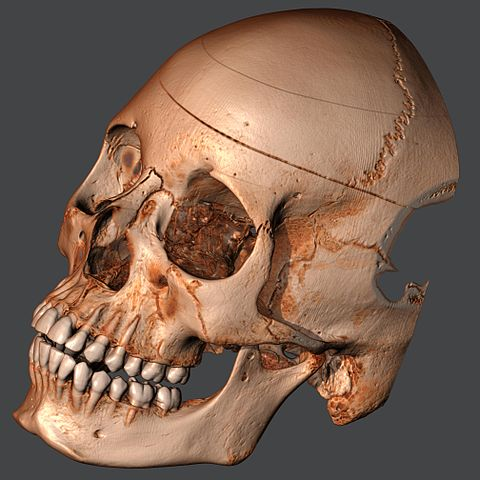
\includegraphics[width=0.6\textwidth]{figures/skull_direct_volume_rendering.jpg}
    \end{captionbeside}
\end{figure}
%

%
\subsubsection{Height-Mapping}
%
Height-mapping only works on \ac{2D} data.
%
It essentially means interpreting the scalar value at each point as a height
value and displaying the resulting three-dimensional surface.
%
Because it transforms \ac{2D} information into \ac{3D} information, it is best
suited for interactive settings, where the resulting surface can be rotated and
viewed from all directions.
%

%
\subsubsection{Direct Volume Rendering}
%
Direct volume rendering~\cite{Levoy1988,Drebin1988} is the extension of
color-mapping to \ac{3D} scalar fields.
%
It involves two steps: Applying a transfer function, and accumulating the
resulting colors and opacities along viewing rays to produce an image.
%
The transfer function has to be chosen carefully to reveal the structures in the
data that are interesting, and make the uninteresting parts transparent.
%
Color and opacity values are then accumulated along viewing rays to simulate the
transport of light through a semitransparent medium.
%

%
The shading of a solid surface can be approximated by using the gradient of the
scalar field as the surface normal (see \cref{fig:direct_volume_rendering}).
%
More advanced techniques use a two-dimensional transfer function that also takes
the gradient magnitude into account when deciding the color, opacity and
shading parameters of a point along the viewing ray~\cite{Kindlmann1998}.
%
% subsection scalar_image_based (end)

\subsection{Geometry-Based Methods} % (fold)
\label{sub:scalar_geometry_based}
%
Geometry-based methods extract some geometrical structures from the data and
display these structures.
%
\emph{Isocontours and -surfaces} belong in this category together with
topological features such as \emph{extremal- and saddle points}, as well as
\emph{ridge- and valley lines and -surfaces}.
%

%
\subsubsection{Isocontours and -surfaces}
%
Isocontours and -surfaces are subsets of the scalar field where the
scalar is equal to a constant (iso-) value.
%
In the literature these are also often referred to as \emph{level sets}.
%
They form lines or surfaces that are always closed or end at the domain
boundary, and that never intersect each other.
%
For \ac{2D} scalar fields, it is common to plot contours for several isovalues
at once, which resemble the height lines we know from maps.
%
In \ac{3D}, it is rare to display more than two or three different isosurfaces
at the same time due to occlusion problems.
%

%
\subsubsection{Critical Points}
%
Critical points are points in a scalar field where the gradient becomes zero.
%
As such, they are features of the scalar field's topology.
%
Critical points can be classified by the eigenvalues of the Hessian matrix at
the critical point:
%
If all eigenvalues are positive the point is a minimum, if all are negative it
is a maximum, and if the Hessian has both positive and negative eigenvalues,
the point is a saddle.
%

%
\subsubsection{Ridge- and Valley Lines and -Surfaces}
%
Ridge- and valley lines and -surfaces also belong to the category
of topological features.
%
There is no universal agreed-upon definition for these types of features.
%
The two most common, competing definitions are \emph{watersheds} and
\emph{height ridges}~\cite{Peikert2008,Eberly2012}.
%
Watersheds are global features that separate the scalar field into ``areas of
influence'' of the different minima (or maxima).
%
Imaginine a scalar field as a height field.
%
Starting a gradient descent from two points on the same side of a watershed
will end up in the same minimum.
%
Starting from two points on opposite sides of the watershed will end up in two
different minima.
%

%
Height ridges are defined by a local differential analysis of the scalar field.
%
As such, their computation is less costly, but they do not provide a
space-filling segmentation of the data.
%
Often, computation of raw ridges and valleys produces a lot of small and
insignificant features due to noise.
%
An additional filtering step~\cite{Peikert2008} can be applied to only keep the
most significant lines (see \cref{fig:ridge_valley_lines}).
%
\begin{figure}[t]
    \begin{captionbeside}
        {Filtered ridge and valley lines of a scalar field.
        Ridges are shown in red, valleys in blue. The scalar field is visualized
        using a combination of height mapping (to obtain the shading) and
        isocontours. Image source: Peikert and Sadlo~\cite{Peikert2008}.
        \label{fig:ridge_valley_lines}}
        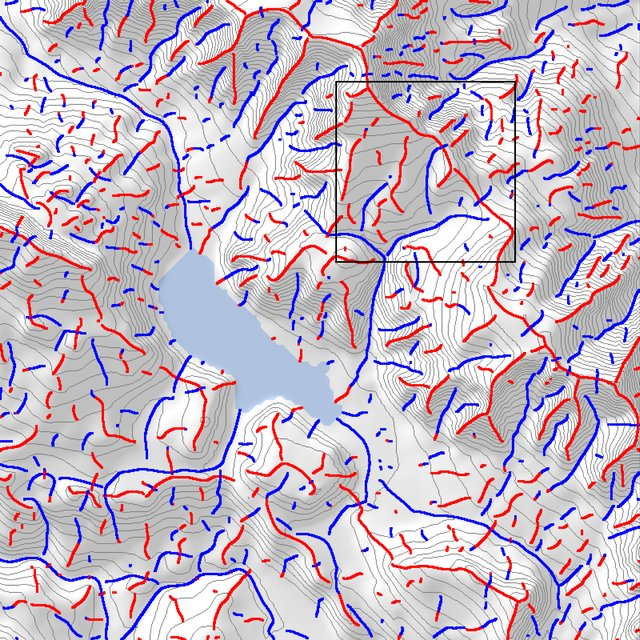
\includegraphics[width=0.6\textwidth]{figures/ridge_valley_lines_peikert.jpg}
    \end{captionbeside}
\end{figure}
%
\subsubsection{Morse-Smale Decomposition} % (fold)
\label{ssub:morse_smale_decomposition}
%
The Morse-Smale Decomposition forms the topological skeleton of a scalar field.
%
It is based on the idea of integral lines of the scalar field.
%
These are maximal paths that are everywhere tangent to the gradient of the
scalar field (see also integral curves in vector fields,
\cref{sub:integral_curves_and_surfaces}).
%
Integral lines always connect two critical points or end at the domain boundary.
%

%
The Morse-Smale decomposition separates the scalar field into a disjoint set of
cells whose union is the whole domain.
%
Each cell is defined as the set of all integral lines that connect the same
minimum and maximum.
%
In this sense, the Morse-Smale decomposition is closely related to the idea of
watersheds:
%
The boundarties of the cells are precisely the watersheds of the scalar field
and its negative.
%
% subsubsection morse_smale_decomposition (end)
%
% subsection scalar_geometry_based (end)
%
% subsection visualization_methods_for_scalar_fields (end)
%
% section scalar_fields (end)
%
\section{Vector Field Visualization} % (fold)
\label{sec:vector_fields}
%
A vector field $\vv(\vx,t): D \times T \mapsto \RRSet^n$ is a map from spatial
and temporal domains $D \subset \EESet^n$ and $T \subset \RRSet$ to the
$n$-dimensional vector space $\RRSet^n$.
%
Just like a scalar field, it assigns a value to each position and time in the
domains, but this time the value is a vector.
%
Examples for vector fields are the velocity of a fluid flow, the displacement
field of a deformed object, and the magnetic field around an electromagnet.
%
If the vector field does not change with time, or we are only interested in the
field at a single instant, we say that we have a \emph{steady} vector field
$\vv(\vx)$.
%
If the vector field changes with time, we call it an \emph{unsteady} vector
field.
%
If we are talking about a vector field representing the velocity of a fluid
flow, we sometimes call it a (steady or unsteady) \emph{flow field}.
%

%
Vector field visualization methods can be sorted into roughly six different
classes: Basic methods, image-based methods, integral curves and -surfaces,
topological features, vortex extraction and \acl{LCS}.
%
We will again visit the most important methods in the following sections.
%

%
\subsection{Basic Methods} % (fold)
\label{sub:vector_basic}
%
Basic methods display the vector data using simple techniques, much like
image-based methods for scalar fields.
%
They encompass techniques such as \emph{arrow plots}, or \emph{color-mapping}
the velocity magnitude, vorticity and other derived quantities directly.
%

%
\subsubsection{Arrow Plots}
%
Arrow plots are the simplest way to visualize a vector field.
%
In such a plot, arrow glyphs are placed at multiple locations throughout the
domain.
%
The arrows are aligned with the direction of the local vector, and their
length is typically scaled based on its magnitude.
%
Such plots can very accurately show the vectors at a limited number of
locations, but they quickly become cluttered once too many arrows are plotted,
or the arrows become too long and occlude each other.
%

%
\subsubsection{Color-Mapping}
%
Color-mapping can be applied to vector fields in different ways.
%
The most common one is simply displaying the magnitude of the vector field as a
scalar.
%
Other scalars derived from the vector field, such as the vorticity magnitude and
divergence, can be visualized in the same way.
%
All of this obviously goes along with a loss of information.
%
Since color has three degrees of freedom, a vector field can also be visualized
without information loss by directly mapping the vector values to colors.
%
The most naive way is to simply interpret the three components of a \ac{3D}
vector as RGB values.
%
Such images theoretically contain they full information of the original vector
field.
%
However, they are very hard to interpret, as there is no inherent meaningful
connection between the direction of the vector and the color it is mapped to.
%
This can be slightly improved for \ac{2D} vector fields by mapping the angle
and magnitude of the vector to hue and value of the HSV color space.
%
% subsection direct_methods (end)
%
\subsection{Image-Based Methods} % (fold)
\label{sub:vector_image_based}
%
Image-based methods visualize the vector data by generating a space-filling
texture.
%
Among such methods are \emph{line integral convolution}, \emph{spot noise},
and \emph{texture advection}.
%

%
\subsubsection{Line Integral Convolution}
%
Line integral convolution (\acs{LIC}\acused{LIC})\cite{Cabral1993} is the most
popular image-based vector field visualization method.
%
It is based on ``smearing'' a random noise texture along stream lines of a
\ac{2D} vector field.
%
More specifically, the color at a certain position is determined as a weighted
integral of the color values encountered along a stream line passing through
that position.
%
The result is a space-filling image where the direction of the vector field is
visible at each location (see \cref{fig:lic_topo}).
%
The basic \ac{LIC} technique is only applicable to \ac{2D} steady vector fields,
but extensions have been developed for \ac{3D}~\cite{Rezk-Salama1999} and
unsteady~\cite{Shen1997} datasets.
%

%
\subsubsection{Spot Noise}
%
Spot noise is also a method designed for \ac{2D} data and produces results
similar to \ac{LIC}~\cite{Wijk1991,Leeuw1995}.
%
It works by blending noise sprites that have been stretched and rotated
according to the local vector direction.
%
In contrast to \ac{LIC}, spot noise better represents the local vector
magnitude, but in regions with low magnitude, the vector direction is not well
visible.
%

%
\subsubsection{Texture Advection}
%
Texture advection works on \ac{2D} steady and unsteady vector fields.
%
It is best suited for vector fields representing a flow, as it simulates the
transport(advection) of a texture with the flow.
%
A texture is placed in the flow at some point in time, and each point on the
texture is moved with the flow over time.
%
As time progresses, the texture is warped, and the viewer can follow where each
part of the texture is transported.
%
This method has a lot in common with the integration-based methods presented in
the next section.
%
In fact, texture advection simply displays a time surface with a mapped texture
in a \ac{2D} vector field.
%

%
% subsection vector_image_based (end)
%
\subsection{Integral Curves and -Surfaces} % (fold)
\label{sub:integral_curves_and_surfaces}
%
Integral curves and -surfaces are generated by integrating the vector field
starting from different kinds of seed structures.
%
Depending on the seeding strategy and the kind of vector field, we can obtain
\emph{streamlines}, \emph{pathlines}, \emph{streaklines}, \emph{timelines},
and the accompanying surfaces\ToCite{Batchelor}.
%
Since integral structures play an important role in several parts of this
thesis, we will cover them here in more detail.
%
\begin{figure}[t]
    \centering
    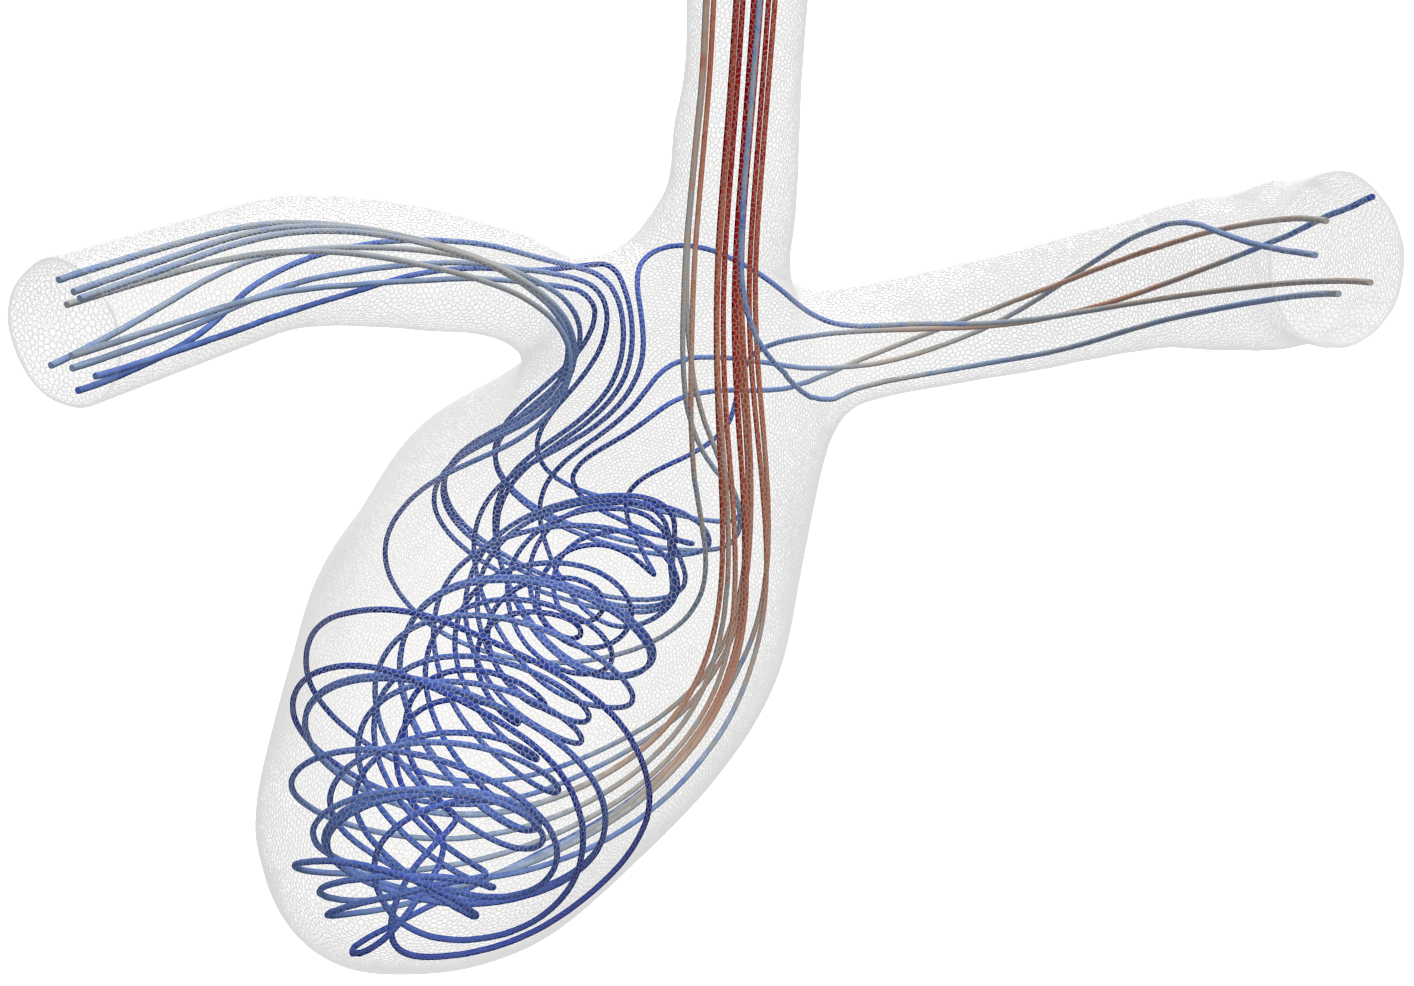
\includegraphics[width=0.9\textwidth]{figures/pathlines_aneurysm.png}
    \caption{Streamlines in the simulated flow through a cranial aneurysm.
             Image courtesy of Tim Gerrits~\cite{Gerrits2018}.}
    \label{fig:streamlines}
\end{figure}
%

\subsubsection{Streamlines} % (fold)
\label{ssub:streamlines}
%
Streamlines are the simplest form of integral curve in a vector field.
%
They are defined for steady vector fields.
%
Depending on the application area, they are also sometimes called \emph{field
lines}.
%
A streamline is a curve that is tangent to the vector field everywhere along its
path.
%
Given a streamline $\vc(s)$ of the steady vector field $\vv(\vx)$, this means
that $\vc(s) \times \vv(\vc(s))$ is $\vNull$ for all $s$.
%
This criterion is valid for any parameterization of the curve, but we can only
use it to check if a given curve is a streamline.
%
To compute streamlines, we typically solve the ordinary differential equation
%
\begin{equation*}
    \frac{\partial \vc(s)}{\partial s} = \vv(\vc(s))
    \text{, with } \vc(0) = \vx_0 \, \text{.}
\end{equation*}
%
This yields a streamline with a particular parameterization: an integral curve
of the vector field.
%
Due to their definition, two stream lines never intersect at single points.
%
They are either completely disjoint, or they coincide.
%

%
Visualizing a steady vector field with stream lines shows the direction of the
flow much like a \ac{LIC} image does, but not in a space-filling manner.
%
This allows for use of streamlines also in \ac{3D} data (see
\cref{fig:streamlines}).
%
Streamline visualization can be deceiving when used on single time slices of
an unsteady flow field.
%
The connected lines mistakenly suggest paths of fluid elements.
%
However, if the flow field changes significantly with time, the actual paths of
fluid elements can deviate significantly from the streamlines in a single time
slice.
%
In this case, the more appropriate visualization tools are pathlines,
streaklines, and timelines, which incorporate the temporal information of the
flow.
%
% subsubsection streamlines (end)

\subsubsection{Pathlines} % (fold)
\label{ssub:pathlines}
%
Pathlines describe the paths of massless particles moving with a
flow.
%
They are defined as the solution to the ordinary differential equation
%
\begin{equation*}
    \frac{\partial \vc(t)}{\partial t} = \vv(\vc(t), t)
    \text{, with } \vc(t_0) = \vx_0 \, \text{,}
\end{equation*}
%
where $\vc(t)$ is the curve of the pathline, $t$ is time, and $\vv(\vx, t)$ is
an unsteady vector field.
%
Looking at this definition, it becomes apparent that for a steady vector field,
which does not change with time, streamlines and pathlines are identical.
%

%
The set of all pathlines for all possible combinations of start position
$\vx$, start time $t_0$ and end time $t$ forms the \emph{flow map}.
%
This function, which we write as $\bPhi(\vx, t_0, t)$, determines where a
massless particle starting at position $\vx$ and time $t_0$ ends up after
advecting with the flow until time $t$.
%

%
Pathlines allow the visualization of the dynamic behavior of an unsteady flow
in a static image.
%
To show the temporal information, the time is often color-mapped on the curve.
%
Unlike streamlines, pathlines can and do intersect each other.
%
For very complex flows, showing a lot of pathlines can therefore quickly become
confusing.
%
In such cases it can be better to show animated streaklines instead.
%
% subsubsection pathlines (end)

\subsubsection{Streaklines} % (fold)
\label{ssub:streaklines}
%
Streaklines are the connected locations of a continuously injected
stream of massless particles into a flow.
%
They approximate the behavior of a thin stream of dye injected at a certain
position that is often applied in experimental settings to visualize the flow.
%
Formally, a streakline is formed by the connected endpoints of a set of
pathlines with the same start position and end time, but continuously increasing
start time.
%
Using the flow map $\bPhi$, which we introduced earlier, we can formally define
a streakline as
%
\begin{equation*}
    \vc(s) = \bPhi(\vx, s, t)\,\text{,}
\end{equation*}
%
where $t$ is the current time, $\vx$ is the injection point, and $s$ is the
continuously increasing start time that runs along the curve.
%
Like pathlines, streaklines also become identical to streamlines if the flow
does not change with time.
%

%
While a pathline shows the behavior of the flow over a period of time, a
streakline only ever shows the position of the injected particles at a
single time instant.
%
Streaklines are therefore often animated by continuously increasing the end
time $t$ and injecting more particles.
%
This again mirrors the behavior of injected dye observed in an experiment.
%
% subsubsection streaklines (end)

\subsubsection{Timelines} % (fold)
\label{ssub:timelines}
%
Timelines are different from all the previous integral lines in that
their seeding structure is not a single point, but a whole line.
%
A timeline is formed by placing a line somewhere in the flow, treating it as a
set of massless particles, and letting the whole line advect with the flow at
once.
%
Formally, a time line is formed by the connected endpoints of a set of pathlines
with the same start and end time, but continuously changing start position.
%
Given a seed curve $\vs(s)$ and start and end times $t_0$ and $t$, we can
formally define a timeline in terms of the flow map as
%
\begin{equation*}
    \vc(s) = \bPhi(\vs(s), t_0, t)\,\text{.}
\end{equation*}
%
Much like streaklines, timelines are often animated to show the progressive
effect of the flow.
%
As the end time $t$ advances, the line is transported and warped by the flow and
visualizes the way the flow mixes and perturbs a region of the fluid.
%
\begin{figure}[t]
    \centering
    \MissingFigure{Image illustrating relationship between pathlines,
    streaklines and timelines}
    \caption{Pathlines, streaklines and timelines of a \ac{2D} vector field.}
    \label{fig:path_streak_timelines}
\end{figure}
%
% subsubsection timelines (end)

\subsubsection{Integral Surfaces} % (fold)
\label{ssub:integral_surfaces}
%
Integral surfaces can be formed from any of the integral lines by using a
higher-dimensional seeding structure.
%
For stream-, path-, and streaklines this means using a line as the seeding
structure.
%
Timesurfaces are formed by using a surface as the seed.
%
Integral surfaces can be helpful for visualization because they have a better
visual coherency than a number of single lines.
%
The curvature, wrinkling and folding of structures induced by the flow become
easier to grasp when using integral surfaces.
%
On the flip side, integral surfaces have more of a problem with occlusion
compared to lines, as they are more massive.
%
% subsubsection integral_surfaces (end)

%
% subsection integral_lines_and_surfaces (end)
%
\subsection{Vector Field Topology} % (fold)
\label{sub:vector_field_topology}
%
% The topology of a vector field is defined by \emph{critical points},
% \emph{boundary switch points/lines}, \emph{attachment- and detachment
% points/lines}, the accompanying \emph{separatrices} connecting these points,
% and \emph{isolated closed streamlines}.
%
The topology of a vector field is defined by \emph{critical points},
\emph{separation- and attachment points} and the accompanying
\emph{separatrices} connecting them.
%
Together, they form a sort of skeleton of the vector field, from which the
behavior of the full field can be inferred.
%
\begin{figure}[t]
    % \centering
    \begin{captionbeside}
        {\ac{LIC} of a \ac{2D} vector field with overlaid vector field topology
        consisting of critical points, boundary switch points, and separatrices.
        Image source: Tino Weinkauf~\cite{Weinkauf2008}.\label{fig:lic_topo}}
        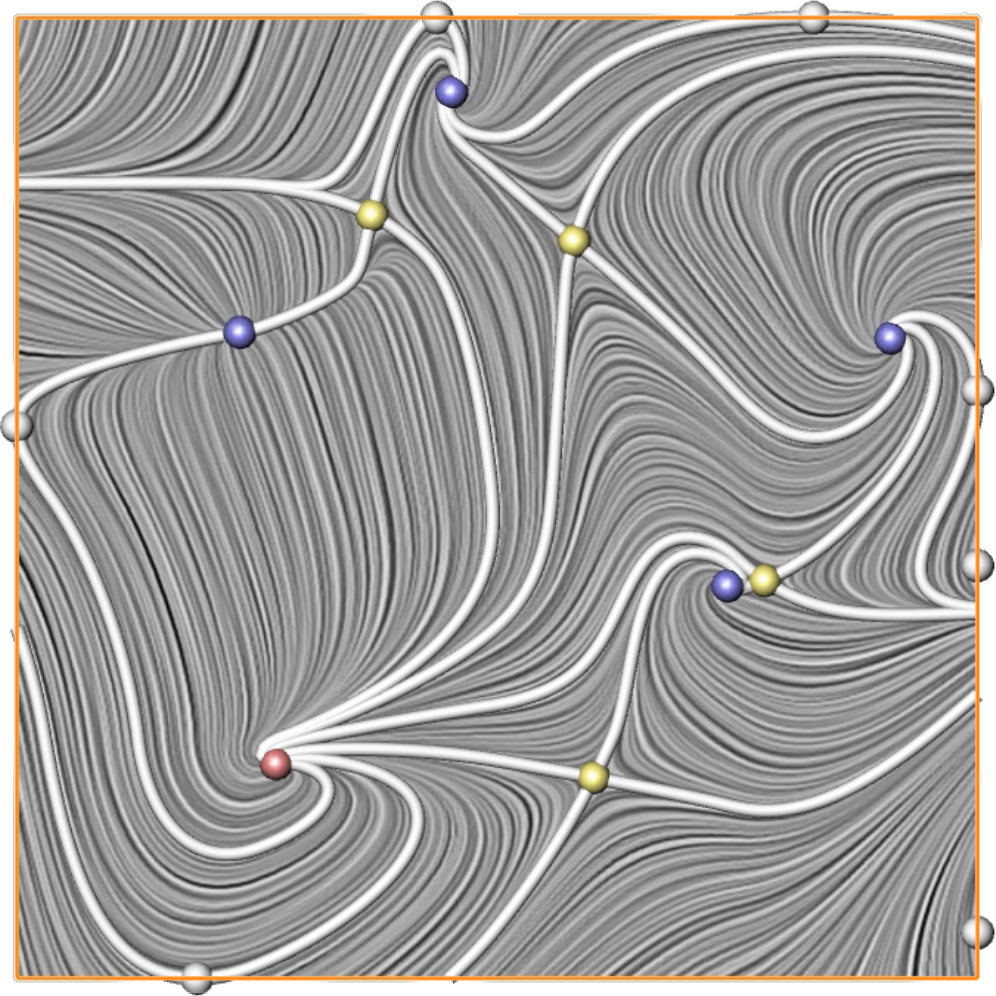
\includegraphics[width=0.6\textwidth]{figures/lic_topology.png}
    \end{captionbeside}
\end{figure}
%

\subsubsection{Critical Points} % (fold)
\label{ssub:critical_points}
%
Critical points of a vector field are locations where the magnitude
of the vector becomes zero.
%
They are interesting because they are at the centers of interesting structures
in the vector field.
%
Critical points in vector fields can be sorted into different categories.
%
Which category a critical point belongs to depends on the behavior of the vector
field in its vicinity, which is encoded in its derivative.
%
The Jacobian matrix $\mJ(\vv) = \vv \T{\nabla}$ gathers the partial derivatives
of all components of the vector field.
%
The signs of the real parts of its eigenvalues indicate if the vector field is
attracting or repelling in the vicinity of the critical point.
%
Depending on these signs, the critical point can be categorized into
\emph{sinks} (negative), \emph{sources} (positive), and \emph{saddles} (mixed
signs).
%
The presence of an imaginary part of the eigenvalues/eigenvectors indicates
swirling behavior.
%
A more in-depth discussion of critical points in vector fields has been provided
by Helman and Hesselink~\cite{Helman1991}.
%
% subsubsection critical_points (end)

%
% \paragraph{Boundary switch points/lines} are locations where the vector field
% is parallel to the boundary of the domain.
% %
% They separate inflow and outflow boundary regions.
% %

\subsubsection{Separation- and Attachment Lines/Surfaces} % (fold)
\label{ssub:separation_attachment_lines}
%
Separation- and attachment lines/surfaces occur on no-slip boundaries.
%
They are locations where the flow separates from/attaches to a surface.
%
In a \ac{2D} flow, these are points.
%
In \ac{3D}, they can be point or line structures.
%
Separation- and attachment structures are similar to critical points of the
vector field, specifically to saddles, in that they are end points of
streamlines of the vector field.
%
However, they are not exactly critical points, as the velocity is zero
everywhere on a no-slip boundary.
%
Instead, they are topological features of the skin friction field, which
describes the shear of the flow near the boundary~\cite{Surana2006}.
%
% subsubsection separation_attachment_lines (end)

\subsubsection{Separatrices} % (fold)
\label{ssub:separatrices}
%
Separatrices connect critical points with each other.
%
They are lines in \ac{2D} vector fields and can be lines or surfaces in \ac{3D}
vector fields~\cite{Helman1989,Helman1991}.
%
Separatrices start at saddle points or separation-/attachment points.
%
They are streamlines with a special property: Streamlines passing through two
points on opposite sides of the separatrix will diverge from each other near a
saddle or separation-/attachment point in forward or backward flow direction.
%
As such, they separate the flow into distinct regions that streamlines starting
in these regions will never leave.
%
Because streamlines and separatrices are an instantaneous observation (they
exist in steady vector fields or at single points in time in an unsteady vector
field), this does not imply that pathlines will never leave these regions in
unsteady flow.
%
For unsteady flows, the equivalent of separatrices are \acl{LCS}, which we will
cover in the next section.
%
% subsubsection separatrices (end)
%
% subsection vector_field_topology (end)
%
\subsection{Vortex Extraction} % (fold)
\label{sub:vortex_extraction}
%
Vortices are structures in a flow that show a swirling motion around a common
center.
%
They will usually stay intact for long periods of time.
%
Vortices are the defining characteristic of turbulent flow.
%
The study of their behavior is a central topic of current fluid dynamics
research.
%
Even though the concept of a vortex seems rather simple, hundreds of years of
fluid dynamics research still has not resulted in a universally accepted formal
definition.
%
This is why there is a plethora of methods for detecting and quantifying
vortices in the literature.
%
Most methods can be sorted into two categories: \emph{region-based} and
\emph{line-based}.
%
They can be further classified by their invariance to transformations of the
reference frame through which the flow is observed.
%
Non-invariant methods are sensitive to all reference frame transformations.
%
Galilean invariant methods are insensitive to any motion of the reference frame
with constant speed and direction.
%
Objective methods are insensitive to any smooth translation and rotation of the
reference frame.
%
We will cover some significant vortex extraction methods here.
%
An extensive survey on the subject has been done by G\"unther and
Theisel~\cite{Guenther2018}.
%

%
Region-based methods measure the ``vortex-ness'' of the flow at a point by a
scalar quantity.
%
Applying a threshold to this quantity shows the vortex regions.
%
Notable representatives of this category are the \emph{vorticity magnitude},
\emph{$\lambda_2$-criterion} and \emph{Q-criterion}, which are all Galilean
invariant methods that work on steady vector fields.
%
Recently, the \emph{\acl{IVD}}~(\acs{IVD}) has been proposed as an objective
criterion for steady vector fields.
%
Its extension, the \emph{\acl{LAVD}}~(\acs{LAVD}) also accounts for unsteady
behavior of the flow.
%
Region-based approaches are generally simple and efficient to implement, but the
results are dependent on the choice of the threshold, and they do not produce
explicit representations of the vortices.
%

%
Line-based methods explicitly extract the vortex core line that is the center
of the swirling behavior.
%
The \emph{reduced velocity} approach for extracting vortex core lines in steady
flows was proposed by Sujudi and Haimes~\cite{Sujudi1995} and later identified
as an application of the \emph{parallel vectors} operator by Peikert and
Roth~\cite{Peikert1999}.
%
This approach is only Galilean invariant when applying it to \ac{2D} vector
fields.
%
A Galilean invariant approach for finding the \emph{cores of swirling particle
motion} in unsteady flows was proposed by Weinkauf \etal \cite{Weinkauf2007}.
%
Recently, G\"unther \etal~\cite{Guenther2017} provided a framework for
objective vortex core detection.
%
This is realized by determining a locally \emph{near-steady frame} for observing
the flow.
%
\begin{figure}[t]
    \centering
    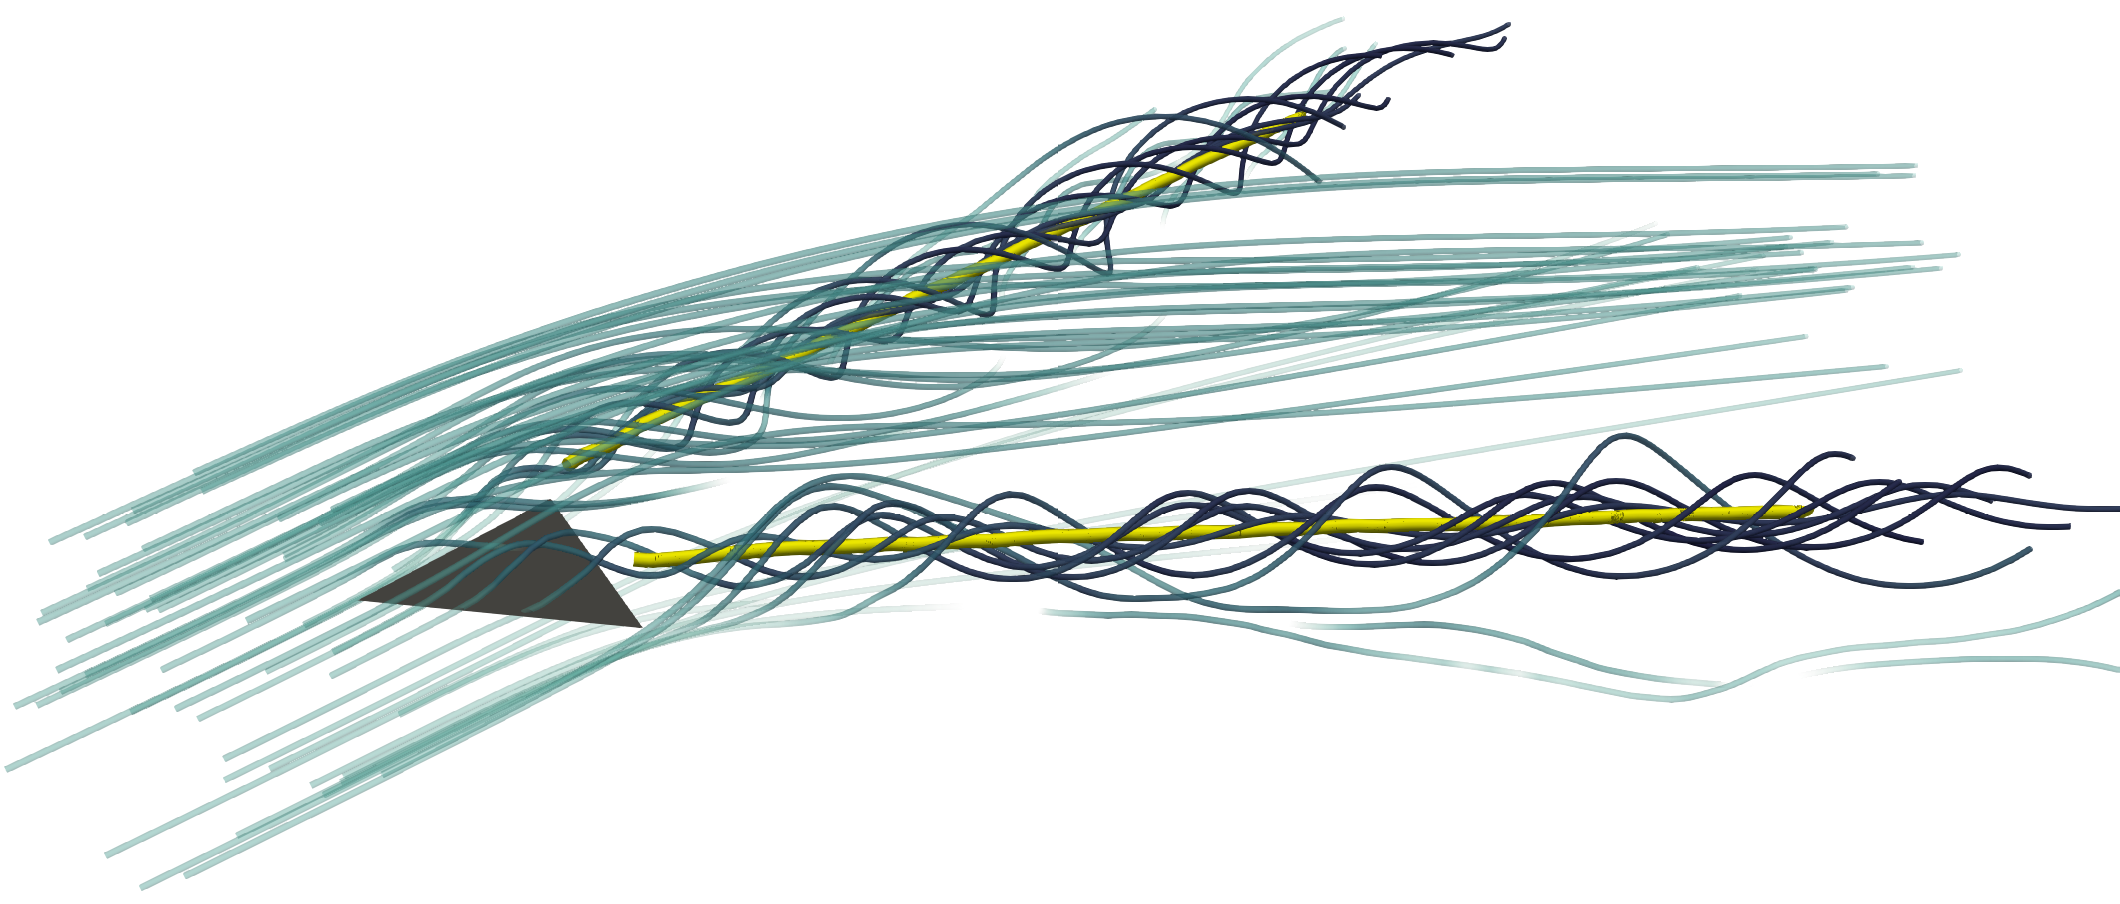
\includegraphics[width=\linewidth]{figures/DeltaWingStreamlines.png}
    \caption{Vortex core lines (yellow) and streamlines (blue) in the steady
    flow around a delta wing.}
    \label{fig:delta_wing_vortex_cores}
\end{figure}
%

%
\subsubsection{Vorticity Magnitude} % (fold)
\label{ssub:vorticity_magnitude}
%
The vorticity is commonly used in fluid dynamics literature to characterize the
rotational behavior of the flow.
%
It is defined as the curl of the flow field $\nabla \times \vv$.
%
The result is a vector field that points in the direction of the local axis of
rotation and whose magnitude indicates the rotation strength.
%
Vorticity magnitude is sometimes used to detect vortices.
%
However, a constant threshold over the whole domain is often not sufficient to
detect and distinguish all vortices, and it might yield false-positives in shear
flow.
%
This is why other methods often perform better.
%
% subsubsection vorticity_magnitude (end)
%
\subsubsection{Q-Criterion} % (fold)
\label{ssub:q_criterion}
%
The Jacobian $\mJ$ of a flow field can be decomposed into a symmetric part $\mS$
(often called \emph{strain rate tensor}) and an asymmetric part $\bOmega$ (often
called \emph{vorticity tensor}) where
%
\begin{equation*}
    \mS = \frac{\mJ + \T{\mJ}}{2}\text{,}\quad
    \bOmega = \frac{\mJ-\T{\mJ}}{2}\text{.}
\end{equation*}
%
For divergence-free (\ie, incompressible) flows, the Q-criterion states that a
region belongs to a vortex if the vorticity tensor is stronger than the strain
rate tensor, \ie,
%
\begin{equation*}
    (\Norm{\bOmega}^2 - \Norm{\mS}^2) > 0 \, \text{.}
\end{equation*}
%
The resulting regions are not as sensitive to the scaling of the data as the
vorticity magnitude.
%
% subsubsection q_criterion (end)
%
\subsubsection{$\bm{\lambda_2}$-Criterion} % (fold)
\label{ssub:lambda_2}
%
The $\lambda_2$-criterion~\cite{Jeong1995} uses invariants of the Jacobian to
detect pressure valleys in incompressible flows.
%
It identifies vortex core regions by investigating the eigenvalues of the tensor
$\mS^2+\bOmega^2$.
%
If the local tensor has at least two negative eigenvalues (\ie, if the middle
eigenvalue $\lambda_2$ is smaller than zero), a point is considered to belong to
a vortex core region.
%
In most cases, $\lambda_2$-criterion and Q-criterion yield similar results.
%
% subsubsection lambda_2 (end)
%
\subsubsection{\acs{IVD}/\acs{LAVD}} % (fold)
\label{ssub:ivd_lavd}
%
Recently, Haller \etal~\cite{Haller2016} proposed the \acf{IVD} as an objective
vortex measure for steady flow fields.
%
It is based on the observation that while the vorticity itself is not objective,
the difference between two vorticity vectors is.
%
Based on this, they define the \ac{IVD} as the difference of the local vorticity
to the average vorticity in a local neighborhood.
%
The \ac{LAVD} extends this to unsteady flows by integrating the \ac{IVD} along
a pathline over a certain time interval.
%
% subsubsection ivd_lavd (end)
%
\subsubsection{Reduced Velocity/Parallel Vectors} % (fold)
\label{ssub:reduced_velocity_parallel_vectors}
%
The first line-based method we present here was proposed by Sujudi and
Haimes~\cite{Sujudi1995} and works on steady flow fields.
%
It is based on the observation that vortex centers look like critical points
when looking at a slice of the vector field that is orthogonal to the vortex
core line.
%
In regions with swirling flow, the Jacobian has two complex conjugate and one
real eigenvector, which points along the local axis of rotation.
%
The reduced velocity or Sujudi/Haimes criterion therefore states that a vortex
core line is located where the projection of the local velocity onto a plane
orthogonal to the single real eigenvector is zero.
%
Peikert and Roth~\cite{Peikert1999} later discovered that this is equivalent to
locations where the velocity vector $\vv$ is parallel to its acceleration
$\mJ\vv$, and so is an application of the \ac{PV} operator, which does not
require the explicit computation of eigenvectors.
%
Defining the criterion in this way, it is equivalent to finding locations where
stream lines have locally vanishing curvature.
%
% subsubsection reduced_velocity_parallel_vectors (end)
%
\subsubsection{Cores of Swirling Particle Motion} % (fold)
\label{ssub:cores_of_swirling_particle_motion}
%
The method of Sujudi/Haimes only considers steady flow fields, or instantaneous
snapshots of unsteady flows.
%
This means that this method finds the centers of swirling streamlines.
%
In unsteady flows, streamlines and pathlines appear to swirl around different
cores if the vortex moves over time (see
\cref{fig:cores_of_swirling_particle_motion}).
%
Weinkauf \etal~\cite{Weinkauf2007} therefore developed an approach to find the
cores of swirling pathlines in unsteady flows.
%
They express pathlines as streamlines in a flow field with one more dimension
where time has been included as an additional explicit state variable.
%
For \ac{3D} unsteady flows, the pathlines are streamlines in \ac{4D} space-time.
%
They derive a criterion similar to Sujudi/Haimes for \ac{4D} vector fields that
can be reduced to a parallel vectors operation on two derived \ac{3D} vector
fields.
%
\begin{figure}[t]
    \centering
    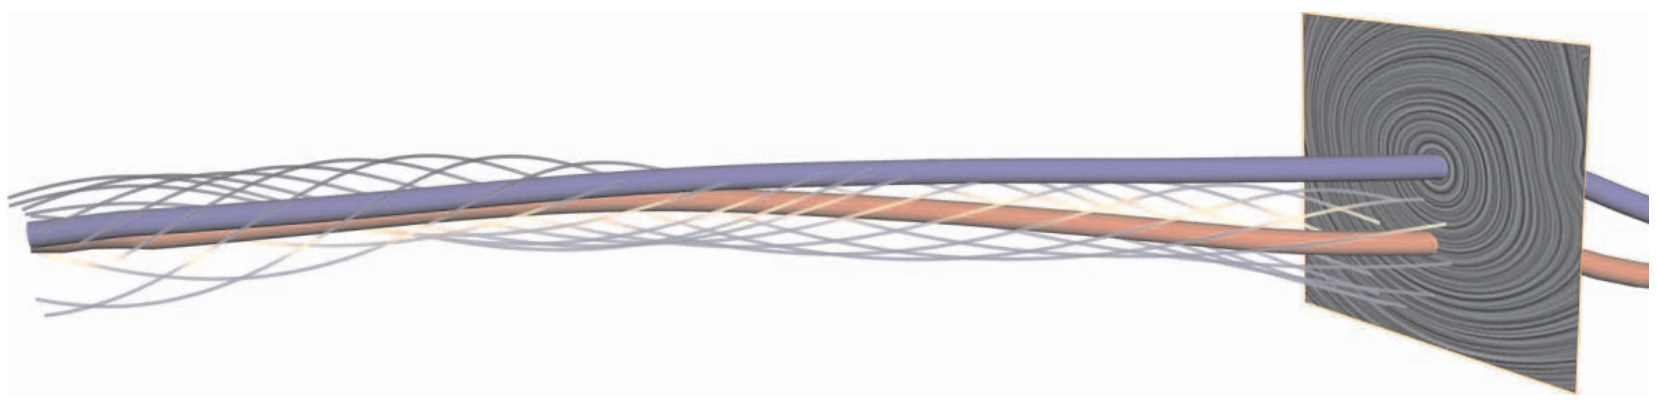
\includegraphics[width=\textwidth]{figures/pathline_streamline_core.png}
    \caption{Streamlines and pathlines swirl around different cores. The red
    tube shows the core of pathlines of a \ac{2D} vector field (rendered in
    \ac{3D} spacetime). The blue tube shows the path of the vortex core
    extracted from the individual time slices. Source: Weinkauf
    \etal~\cite{Weinkauf2007}.}
    \label{fig:cores_of_swirling_particle_motion}
\end{figure}
%
% subsubsection cores_of_swirling_particle_motion (end)
%
\subsubsection{Near-Steady Frame} % (fold)
\label{ssub:near_steady_frame}
%
The optimal reference frame for observing a vortex is a frame that follows the
vortex center over time~\cite{Robinson1991}.
%
In such a frame, the observed vector field around the vortex becomes almost
steady as ambient effects of larger flow structures are eliminated.
%
This is the basis of the approach proposed by G\"unther
\etal~\cite{Guenther2017}.
%
For each point in the flow, a locally optimal reference frame is computed in
which the flow becomes almost steady.
%
The reference frame is determined for a finite-sized neighborhood via a simple
linear optimization.
%
Once the vector field (and its derivatives) have been ``objectified'', any
region- or line-based vortex extractor that is designed for steady vector fields
can be used to extract objective unsteady vortices.
%
% subsubsection near_steady_frame (end)
%
% subsection vortices (end)
%
\subsection{Lagrangian Coherent Structures} % (fold)
\label{sub:lagrangian_coherent_structures}
%
\acf{LCS} are structures that show a locally maximal attracting or repelling
behavior of massless particles.
%
As the name suggests, these structures also tend to stay coherent over longer
time periods.
%
They can be thought of as a counterpart to vortices.
%
Whereas vortices represent the centers of swirling behavior, \ac{LCS} tend to
be located at the boundaries between vortices.
%
They act as transport barriers that have a minimal transverse flux of material
and are therefore very important for the investigation of mixing and transport
processes.
%
There are a number of very different methods for the investigation of \ac{LCS}.
%
A survey and comparison of some notable methods can be found
in~\cite{Hadjighasem2017}.
%

%
One popular approach to detecting \ac{LCS} is the investigation of the local
Lyapunov exponent~\cite{Ott2002}.
%
The Lyapunov exponent describes the rate of separation of infinitesimally close
trajectories over an infinite time interval.
%
Since real-world data is usually finite in time and space, two approximations of
the Lyapunov exponent are commonly used in practice: the
\emph{\acl{FTLE}\acused{FTLE}} (\acs{FTLE})~\cite{Haller2001} and
\emph{\acl{FSLE}\acused{FSLE}} (\acs{FSLE})~\cite{Aurell1997}.
%
It has been shown that ridges of the \ac{FTLE} or \ac{FSLE} field correspond
well to the locations of \ac{LCS}~\cite{Shadden2005,Haller2001}.
%

%
The basis for the computation of both \ac{FTLE} and \ac{FSLE} is the right
Cauchy-Green deformation tensor
%
\begin{equation*}
    \mC(\vx, t_0, t) = \T{\mF(\vx, t_0, t)}\, \mF(\vx, t_0, t) \,\text{,}
\end{equation*}
%
where $\mF$ is the deformation gradient obtained from the derivative of the
flow map
%
\begin{equation*}
    \mF(\vx, t_0, t) = \bPhi(\vx, t_0, t)\T{\nabla}\text{.}
\end{equation*}
%
The Cauchy-Green tensor describes the deformation the infinitesimal neighborhood
of a point $\vx$ at time $t_0$ experiences when advecting with the flow until
time $t$.
%
The maximum eigenvalue $\lambda_{\textnormal{max}}$ of this tensor is a measure for
the maximum separation of two particles starting in this infinitesimal
neighborhood.
%
\subsubsection{Finite-Time Lyapunov Exponent} % (fold)
\label{ssub:ftle}
%
The \acl{FTLE} measures the maximum separation of neighboring particles after
advecting with the flow for a finite time:
%
\begin{equation*}
    \text{FTLE}(\vx, t_0, \tau)
        = \frac{1}{|\tau|}
          \ln\sqrt{\lambda_{\max}\left[\mC(\vx, t_0, t_0 + \tau)\right]}\,\text{.}
\end{equation*}
%

%
A straightforward way of approximating the \ac{FTLE} of a flow is to compute the
flow map $\bPhi$ on a discrete grid and estimate the deformation gradient $\mF$
via central differences.
%
Since the ridges of an \ac{FTLE} field can become very sharp with increasing
integration time $\tau$, this is usually not very accurate.
%
Additionally, we are usually not interested in an accurate estimation of regions
without ridges.
%
For this reason, there are multiple numerical schemes for more precise or
performant \ac{FTLE} computations.
%
A good overview of the existing methods is provided in Alexander Kuhn's PhD
thesis~\cite{Kuhn2013}.
%
\begin{figure}[t]
    \centering
    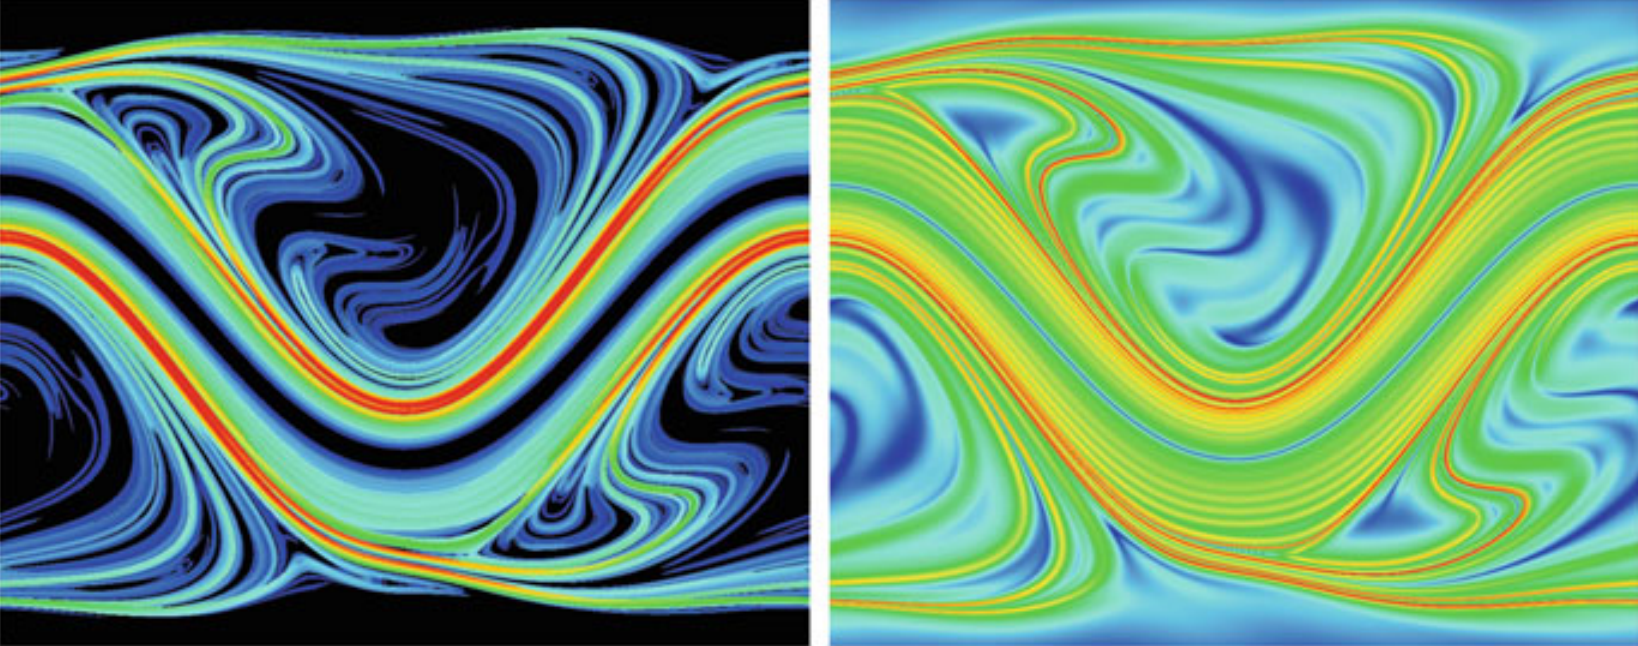
\includegraphics[width=\textwidth]{figures/fsle_ftle_peikert.png}
    \caption{Comparison of \ac{FSLE} (left) and \ac{FTLE} (right) of the flow
    field of a meandering jet. Image source: Peikert \etal~\cite{Peikert2014}.}
    \label{fig:ftle_fsle}
\end{figure}
%
% subsubsection ftle (end)
%
\subsubsection{Finite-Size Lyapunov Exponent} % (fold)
\label{ssub:fsle}
%
The \acl{FSLE} measures the time a pair of infinitesimally close particles
need to separate by a constant amount in space:
%
\begin{equation*}
    \text{FSLE}(\vx, t_0, r) = \frac{1}{|\tau_r|} \ln{r}\,\text{,}
\end{equation*}
%
where $\tau_r$ is the minimum time interval for which
%
\begin{equation*}
    \sqrt{\lambda_{\max}\left[\mC(\vx, t_0, t_0+\tau_r)\right]} = r\,\text{.}
\end{equation*}
%

%
\ac{FSLE} is popular in the oceanography community, but has not been adopted
much in the general visualization community.
%
As a result, \ac{FSLE} computation schemes in the literature are mostly
straightforward.
%
Either the maximum separation $\lambda_{\max}$ is estimated by a discrete
sampling of the flow map in different
directions~\cite{dOvidio2004,Hernandez-Carrasco2011}, or the Cauchy-Green tensor
is estimated based on central differences~\cite{Peikert2014}.
%

%
\ac{FTLE} and \ac{FSLE} yield similar results, given the right parameters (see
\cref{fig:ftle_fsle}).
%
However, their semantic differences might make one or the other more appropriate
depending on the application.
%
While \ac{FTLE} operates on a finite integration time $\tau$, which must be
estimated a-priori, it shows the behavior of the flow for all scales of spatial
separation.
%
In contrast, \ac{FSLE} needs the choice of a separation size, which might be
more intuitive.
%
It yields information about separation at different spatial scales, but it does
not show separation that is smaller than the given threshold $r$.
%
% subsubsection fsle (end)
%
% subsection lagrangian_coherent_structures (end)
%
% section vector_fields (end)
%
\section{Second-Order Tensor Field Visualization} % (fold)
\label{sec:tensor_fields}
%
Although tensors are a very general concept in mathematics, when we talk about
tensor fields in scientific visualization, we generally mean a map $\mT(\vx, t):
D \times T \mapsto \RRSet^{m \times m}$ from spatial domain $D \in \EESet^n$ and
temporal domain $T \in \RRSet$ to the space of second-order tensors which can be
represented by matrices from $\RRSet^{m \times m}$.
%
While a vector describes an effect acting on a point, a second-order tensor
describes an effect on a vector.
%
Often, this means that the tensor describes some sort of differential effect
that acts on the infinitesimal neighborhood of a point.
%
Second-order tensor fields occur in a variety of different scientific contexts.
%
Some examples are stress and strain tensors in mechanical engineering
applications, and diffusion tensors occurring in \ac{DTI}, a special \ac{MRI}
modality used to visualize fiber tracts, \eg, in the human brain.
%
In reality, these tensor fields vary in time.
%
However, in practice datasets with temporally varying tensor fields are
relatively rare, and visualization methods are mostly designed for instantaneous
tensor fields $\mT(\vx)$.
%

%
The most important tensor field visualization methods can be roughly classified
into five different categories:
%
direct, image-based, glyph-based, line-/surface-based and topology-based.
%

\subsection{Direct Methods} % (fold)
\label{sub:tensor_direct_methods}
%
Direct methods display some properties of the tensor directly.
%
Usually, one or more scalar quantities are derived from the vector field and
displayed using methods from scalar field visualization.
%
Notable examples for direct methods are \emph{color-mapping} and \emph{direct
volume rendering}.
%

%
\subsubsection{Color-Mapping} % (fold)
%
Just like scalar and vector fields, \ac{2D} or slices of \ac{3D} tensor fields
can be displayed by color-mapping some scalar properties of the tensor.
%
When investigating mechanical stress tensors, some norm of the tensor is often
displayed.
%
When viewing diffusion tensors from \ac{DTI} data, the \ac{3D} direction of the
major eigenvector is often encoded using a radial or spherical color
map~\cite{Pajevic1999}.
%
Such a visualization is not very intuitive and requires the viewer to be
familiar with the interpretation of the resulting images.
%
% subsubsection color_mapping (end)
%

\subsubsection{Direct Volume Rendering} % (fold)
%
For \ac{3D} data, the equivalent of color-mapping is direct volume rendering.
%
The additional degrees of freedom of a tensor compared to scalar or vector data
means that some information invariably gets lost when using normal direct volume
rendering techniques.
%
This means an intelligent mapping of the tensor to color, opacity and shading
needs to be performed to retain the most important aspects of the data.
%
For diffusion tensors, different possibilities for such mappings have been
explored by Kindlmann \etal{}~\cite{Kindlmann2000}.
%
They base their mappings on the different kinds of anisotropies indicated by the
ratio of the tensor's eigenvalues that can be found in diffusion tensor data
(namely linear anisotropy, planar anisotropy, and isotropy).
%
This produces visualizations that represent the important features in \ac{DTI}
data, but is not necessarily applicable to other application domains.
%
% subsubsection direct_volume_rendering (end)
% subsection direct_methods (end)

\subsection{Image-Based Methods} % (fold)
\label{sub:tensor_image_based}
%
Like the equivalent techniques for vector fields, image-based visualization of
second-order tensor fields works by generating space-filling images that are
derived from the underlying tensor data.
%
Techniques in this category have yet to be adopted into mainstream visualization
tools, so we will only discuss two notable examples: \emph{HyperLIC} by Zheng
and Pang~\cite{Zheng2003} and \emph{LIC with variable input textures} by Hotz
\etal{}~\cite{Hotz2004}.
%
Both techniques are modified versions of \ac{LIC} based on the eigenvectors of
the tensor fields.
%

\subsubsection{HyperLIC} % (fold)
%
HyperLIC was introduced by Zheng and Pang~\cite{Zheng2003} as a visualization
technique for diffusion tensor data.
%
In this data, a central characteristic is the diffusion anisotropy represented
by the ratio of the eigenvalues.
%
While \ac{LIC} accumulates the values of an input texture along streamlines of a
vector field, HyperLIC conceptually accumulates values in a strip- or tube-like
volume that follows the local eigenvector direction and whose cross section is
scaled according to the local eigenvalue ratio.
%
This produces \ac{LIC}-like results in areas with a strongly dominating
eigenvalue, and blurry areas with no sense of direction in isotropic areas where
all eigenvalues are similar.
%
As this technique is designed for diffusion tensors, which are positive
definite, it lacks a way of indicating eigenvalue sign and therefore is not well
suited for the visualization of indefinite tensors.
%
% subsection tensor_image_based (end)

\subsubsection{\ac{LIC} with Variable Input Textures} % (fold)
\label{ssub:lic_with_variable_input_textures}
%
A technique which is better suited for symmetric indefinite tensors, which can
have negative eigenvalues, was presented by Hotz \etal{}~\cite{Hotz2004}.
%
As opposed to HyperLIC, which accumulates the values of the input texture in a
volume instead of along a curve, this method uses a standard \ac{LIC} on the
``eigenvector fields'' of the tensor field.
%
The remaining information in the tensor is visualized by carefully varying the
spot size, spot density and color of the input noise texture as well as the
convolution length based on the local eigenvalues.
%
Images from major and minor eigenvector are overlaid to visualize both at the
same time.
%
\Cref{fig:lic_var_tex} shows an example of this technique applied to a slice
of the stress tensor field from a two point load dataset with a pushing and
pulling force.
%
\begin{figure}[t]
    % \centering
    \begin{captionbeside}{LIC with variable input textures. Image source: Hotz
    \etal{}~\cite{Hotz2004}.\label{fig:lic_var_tex}}
        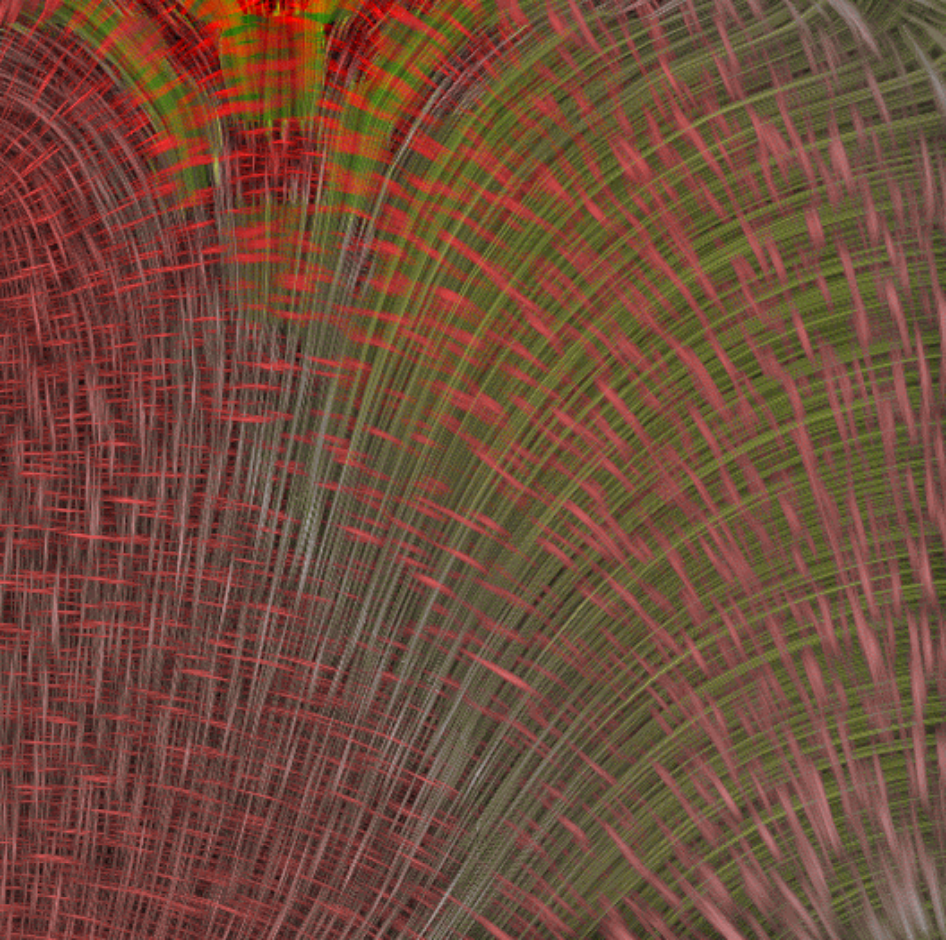
\includegraphics[width=0.6\textwidth]{figures/tensor_lic_variable_texture.png}
    \end{captionbeside}
    % \caption{LIC with variable input textures showing a stress tensor field of a
    % two point load dataset with a pushing and pulling force. Red shows negative
    % eigenvectors (compressive stress), green shows positive eigenvectors
    % (tensile stress). Density, spot size, color intensity and convolution length
    % are varied according to the local eigenvalues. Image source: Hotz
    % \etal{}~\cite{Hotz2004}.}
\end{figure}
%
% subsubsection lic_with_variable_input_textures (end)

\subsection{Glyph-Based Methods} % (fold)
\label{sub:tensor_glyph_based}
%
Glyph-based methods for tensor field visualization place small geometric objects
in space to represent certain characteristics of the local tensor.
%
They have the advantage of being able to display all features of a tensor at
once, but their visual complexity can make them hard to read.
%
Glyph-based methods generally differ by the restrictions they place on the
tensor.
%
There are various glyph designs for \emph{symmetric positive definite},
\emph{symmetric (indefinite)}, and \emph{general tensors} in both \ac{2D} and
\ac{3D}.
%
Some research has also focused on how to place and distribute glyphs to better
emphasize global structures in the data, as opposed to the simple regular
grid-based approach~\cite{Kindlmann2006,Feng2008}.
%

\subsubsection{Symmetric Positive Definite Tensors} % (fold)
%
Symmetric positive definite tensors are tensors that always have positive
real eigenvalues, and whose eigenvectors are orthogonal.
%
The domain most explored in scientific visualization for these tensors is
\ac{DTI} data, where they represent the diffusion of Hydrogen atoms in organic
tissue (specifically in neural fibers of the brain).
%
The simplest glyphs for visualizing such tensors are ellipses~\cite{Basser1996},
cylinders~\cite{Wiegell2000} or boxes~\cite{Schroeder2006}.
%
These glyphs are formed by placing some prototypical base shape (a unit sphere
or cube) centered at the origin and then transforming it according to the
tensor.
%
The resulting glyph is then placed at the sampling position the tensor
originated from.
%
Most often, the glyphs are also scaled to achieve a size fitting with the
glyph density.
%
Such simple glyphs accurately represent how the tensor transforms input vectors
to output vectors.
%
The disadvantage is that they have various visual ambiguities that make their
interpretability less than ideal~\cite{Kindlmann2004}.
%

%
Kindlmann~\cite{Kindlmann2004} solved this problem by carefully designing
glyphs based on superquadrics.
%
These superquadrics change their base shape depending on the relationship of
the three eigenvalues of the tensor.
%
In this way, ambiguities intrinsic to the usage of constant base shapes are
eliminated.
%

\subsubsection{Symmetric Tensors} % (fold)
%
General symmetric tensors always have real orthogonal eigenvectors, but their
eigenvalues can be negative.
%
This poses a challenge for glyph design.
%
Simply transforming a symmetric base shape with the tensor will produce the same
image for eigenvalues with equal magnitude but opposite sign.
%
Different glyphs for symmetric tensors in different application domains have
been proposed in the literature~\cite{Pajevic1999,Hashash2003,Jeremic2002}.
%
Often, color is used to indicate the sign of the eigenvalue.
%
Alternatively, the glyph base shape is modified to represent the difference
between positive and negative eigenvalues.
%
Schultz and Kindlmann~\cite{Schultz2010a} built on top of all of this work to
develop a set of superquadric-based tensor glyphs that clearly indicates
eigenvalue sign by a combination of color and concave shape (see
\cref{fig:tensor_glyphs}).
%
% \begin{figure}[t]
%     \begin{tikzpicture}
%         \node (pos) {
%             \includegraphics[width=0.3\textwidth]{figures/diffusion_tensor_glyphs.png}
%         };
%         \node[anchor=west] (symm) at (pos.east) {
%             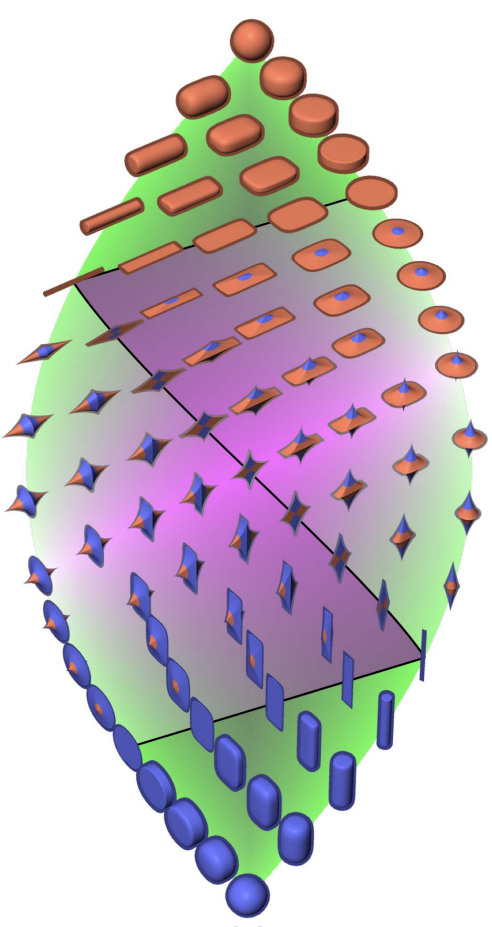
\includegraphics[width=0.3\textwidth]{figures/symmetric_tensor_glyphs.png}
%         };
%         \node[anchor=west] (general) at (symm.east) {
%             \includegraphics[width=0.3\textwidth]{figures/general_tensor_glyphs.png}
%         };
%     \end{tikzpicture}
%     \caption{Superquadric tensor glyphs for symmetric positive definite (left),
%     symmetric indefinite (middle), and general (right) tensors.}
%     \label{fig:tensor_glyphs}
% \end{figure}
%
% \begin{figure}[t]
%     \centering
%     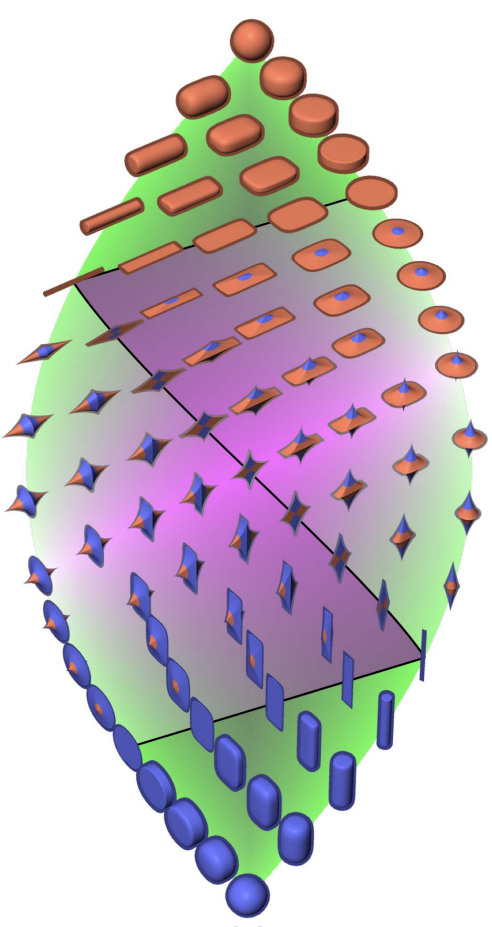
\includegraphics[width=0.5\textwidth]{figures/symmetric_tensor_glyphs.png}
%     \caption{Superquadric glyphs for symmetric tensors. Image source: Schultz
%     \etal{}~\cite{Schultz2010a}.}
%     \label{fig:tensor_glyphs}
% \end{figure}
%
\begin{figure}
    \begin{captionbeside}
        {Superquadric glyphs for symmetric tensors. Includes glyphs for positive
         definite tensors as a subset (top triangle). Image source: Schultz
         \etal{}~\cite{Schultz2010a}.\label{fig:tensor_glyphs}}
        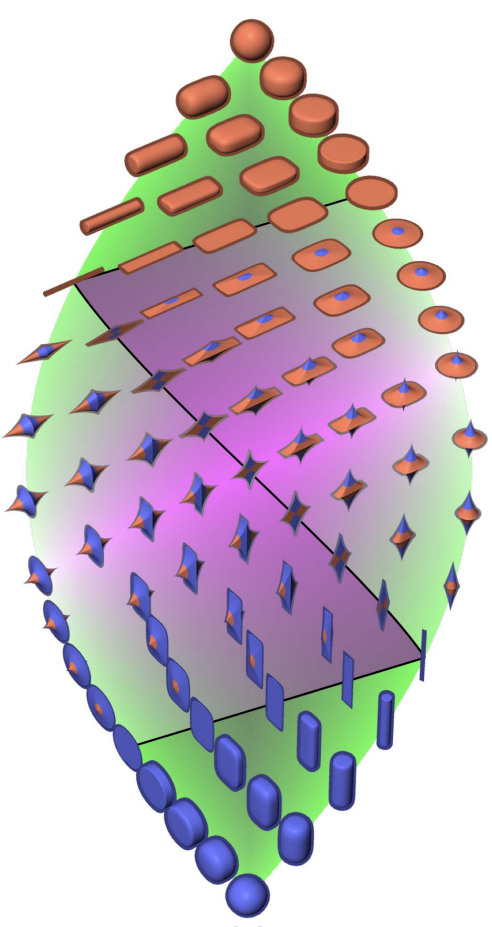
\includegraphics[width=0.4\textwidth]{figures/symmetric_tensor_glyphs.png}
    \end{captionbeside}
\end{figure}

\subsubsection{General Tensors} % (fold)
%
Apart from different eigenvalue signs, the eigenvectors of general (asymmetric)
second-order tensors need not be orthogonal, and they can be complex.
%
Gerrits \etal{}~\cite{Gerrits2017} built on top of the work of Kindlmann, Schultz
\etal{} to design a set of glyphs for general tensors in \ac{2D} and \ac{3D} that
can represent non-orthogonal eigenvectors and additionally incorporates
information about complex eigenvalues via color.
%

\subsection{Line-/Surface-Based Methods} % (fold)
\label{sub:tensor_line_surface_based}
%
Line- and surface-based methods for the visualization of second-order tensor
fields are very similar to integral lines and surfaces for vector fields.
%
They work by considering the eigenvectors of the tensor field as the equivalent
of a vector field and basing the visualization on the resulting field lines.
%
Of course these methods can only visualize real eigenvectors and are therefore
generally applied to symmetric tensor fields only.
%
Because of the differences between real vector fields and eigenvector fields,
modified integration methods are necessary to form these field lines.
%
The most important methods based on this principle are \emph{tensor field
lines}, \emph{hyperstreamlines}, \emph{tensorlines} and
\emph{hyperstreamsurfaces}.
%

\subsubsection{Tensor Field Lines} % (fold)
%
Tensor field lines are lines that are everywhere tangent to an eigenvector of
the tensor field.
%
They are the basis for all the methods in this category.
%
Tensor field lines have been known as \emph{stress trajectories} (see
\cref{fig:stress_trajectories}) in the context of solid mechanics since the
1800s.
%
Early stress visualizations using this technique were drawn by hand based on
photoelastic measurement techniques~\cite{Focht1962,Timoshenko1983}.
%
In a computer, these lines are obtained by integrating a vector field generated
from the eigenvector field by choosing an orientation and magnitude at each
location \cite{Dickinson1989,Tricoche2006}.
%
Since this choice is not always unique in the vicinity of degenerate points
where two or more eigenvalues are equal, special care has to be taken to avoid
a sudden flip of direction.
%
The resulting lines show the continuous change of direction of eigenvectors in
the tensor field, but they are not well suited to judge the magnitude of the
eigenvalues.
%
\begin{figure}[t]
    \centering
    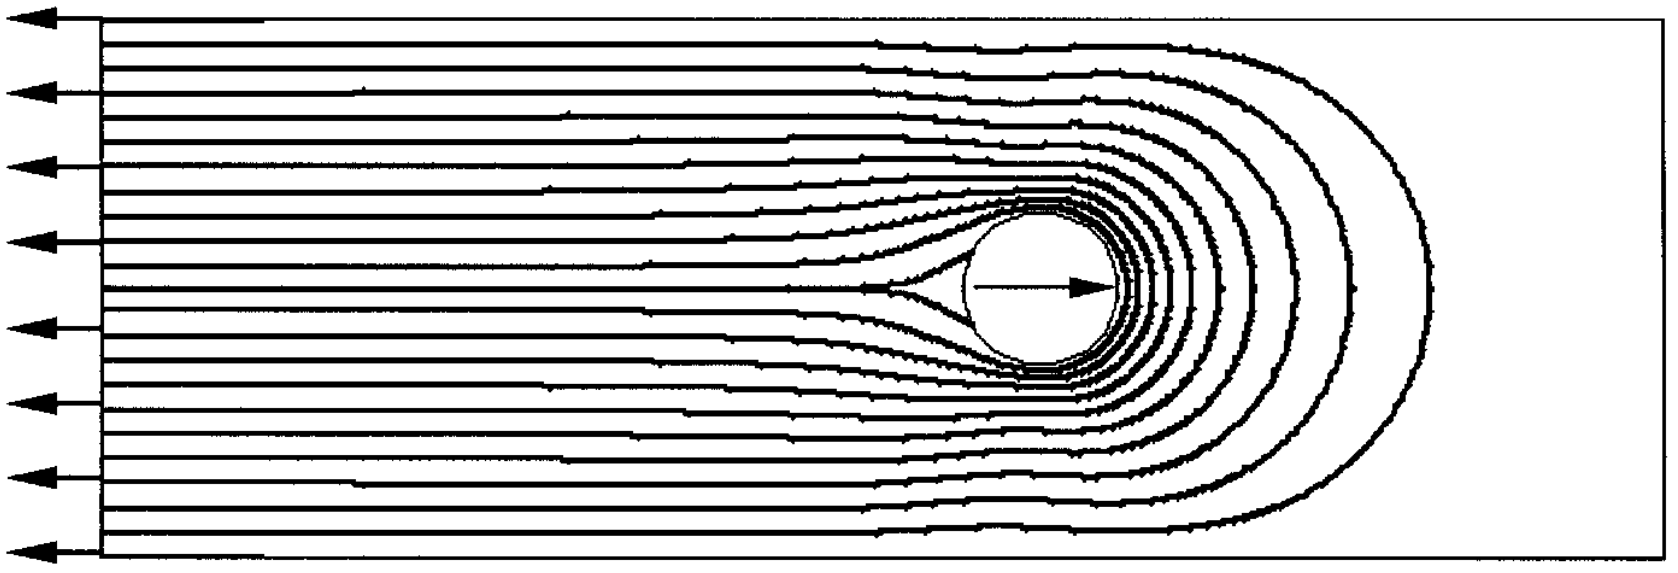
\includegraphics[width=0.8\textwidth]{figures/stress_trajectories.png}
    \caption{Major principal stress trajectories in a plate with a loaded hole.
             Image source: Kelly and Tosh~\cite{Kelly2000}.}
    \label{fig:stress_trajectories}
\end{figure}
%

\subsubsection{Hyperstreamlines} % (fold)
%
To enhance the information content of tensor field line visualizations,
Delmarcelle and Hesselink introduced hyperstreamlines~\cite{Delmarcelle1993}.
%
These hyperstreamlines follow the field lines of one of the eigenvectors of the
tensor field, while their cross-section is a cross shape or ellipse aligned with
the other two eigenvectors and scaled by the corresponding eigenvalues.
%
The eigenvalue corresponding to the eigenvector parallel to the hyperstreamline
is color-coded on the surface.
%
In this way, the full information of the tensors along the hyperstreamlines is
visualized.
%
It is important to note here that the term hyperstreamline is sometimes used
in the literature to mean what we introduced as tensor field lines.
%
In this work, we use it exclusively for lines with a variable cross-section.
%

\subsubsection{Tensorlines} % (fold)
%
In the analysis of diffusion tensor fields obtained from \ac{DTI} scans of the
human brain, tensor field lines are tracked to obtain the paths of neural
fibers.
%
Because this data suffers from noise and partial voluming effects due to limited
resolution, near-isotropic areas can occur where fibers with different
directions cross.
%
In these areas, the eigenvector direction is not clearly defined and often
dominated by noise.
%
Just following the vector field obtained from a single eigenvector will result
in random paths that do not represent the paths of actual brain fibers.
%
To counteract this problem, Weinstein \etal{}~\cite{Weinstein1999} introduced
tensorlines.
%
The core of the algorithm is a modified streamline integration that not only
takes into account the direction of the major eigenvector but is also guided
by the direction of the previous step in near-isotropic regions.
%

\subsubsection{Hyperstreamsurfaces} % (fold)
%
The concept of hyperstreamlines was extended to hyperstreamsurfaces by Jeremi\'c
\etal{}~\cite{Jeremic2002}.
%
They are formed analogous to streamsurfaces by using a curve instead of a point
as a seed structure for integration.
%
In this case, the other eigenvectors and eigenvalues can not be sensibly
displayed by varying a cross section like with hyperstreamlines.
%
Instead, only the eigenvalue of the integrated eigenvector is color-coded on the
surface.
%

\subsection{Topological Methods} % (fold)
\label{sub:tensor_topological}
%
Similar to scalar- and vector fields, topological structures in tensor fields
are defined by some mathematical degeneracy.
%
In contrast to the topology of vector fields, it is not the magnitude of the
tensor that is important, but the relationship between the eigenvalues and
eigenvectors.
%
For symmetric tensor fields, the topology is formed by \emph{degenerate points
and lines} and their \emph{separatrices}, as well as \emph{neutral and traceless
tensors}.
%
For \emph{general (asymmetric) tensor fields}, the topology is formed by
degenerate structures and circular points.
%

\subsubsection{Degenerate Points and Lines} % (fold)
%
The core of topological analysis of symmetric tensor fields are degenerate
structures.
%
These are structures where two eigenvalues are equal, and the eigenvector
directions are not uniquely defined.
%
They are the locations where tensor field lines intersect.
%
In \ac{2D} tensor fields, such structures can be classified into trisector and
wedge points, depending on the behavior of the tensor field lines in their
vicinity.
%
In \ac{3D}, degenerate features form lines.
%
Zheng \etal{}~\cite{Zheng2005b} showed that the type of degenerate point can
switch at isolated points along these lines.
%
These are the points where the degenerate line is parallel to the plane spanned
by the valid eigenvectors corresponding to the dual eigenvalue.
%
Degenerate lines in symmetric tensor fields were first studied by Delmarcelle,
Hesselink \etal{}~\cite{Delmarcelle1994,Hesselink1997}.
%
Numerical algorithms for their robust extraction were developed by Zheng
\etal{}~\cite{Zheng2004,Zheng2005} and later adapted for noisy \ac{DTI} data by
Tricoche \etal{}~\cite{Tricoche2008}.
%
\Cref{fig:tensor_topology} shows the topology of a common test case in
structural mechanics where two point loads are applied to the surface of a solid
block.
%
\begin{figure}[t]
    \begin{captionbeside}
        {Topology of the stress tensor in a double point load dataset. Image
         source: Zheng and Pang~\cite{Zheng2004}.\label{fig:tensor_topology}}[o]
        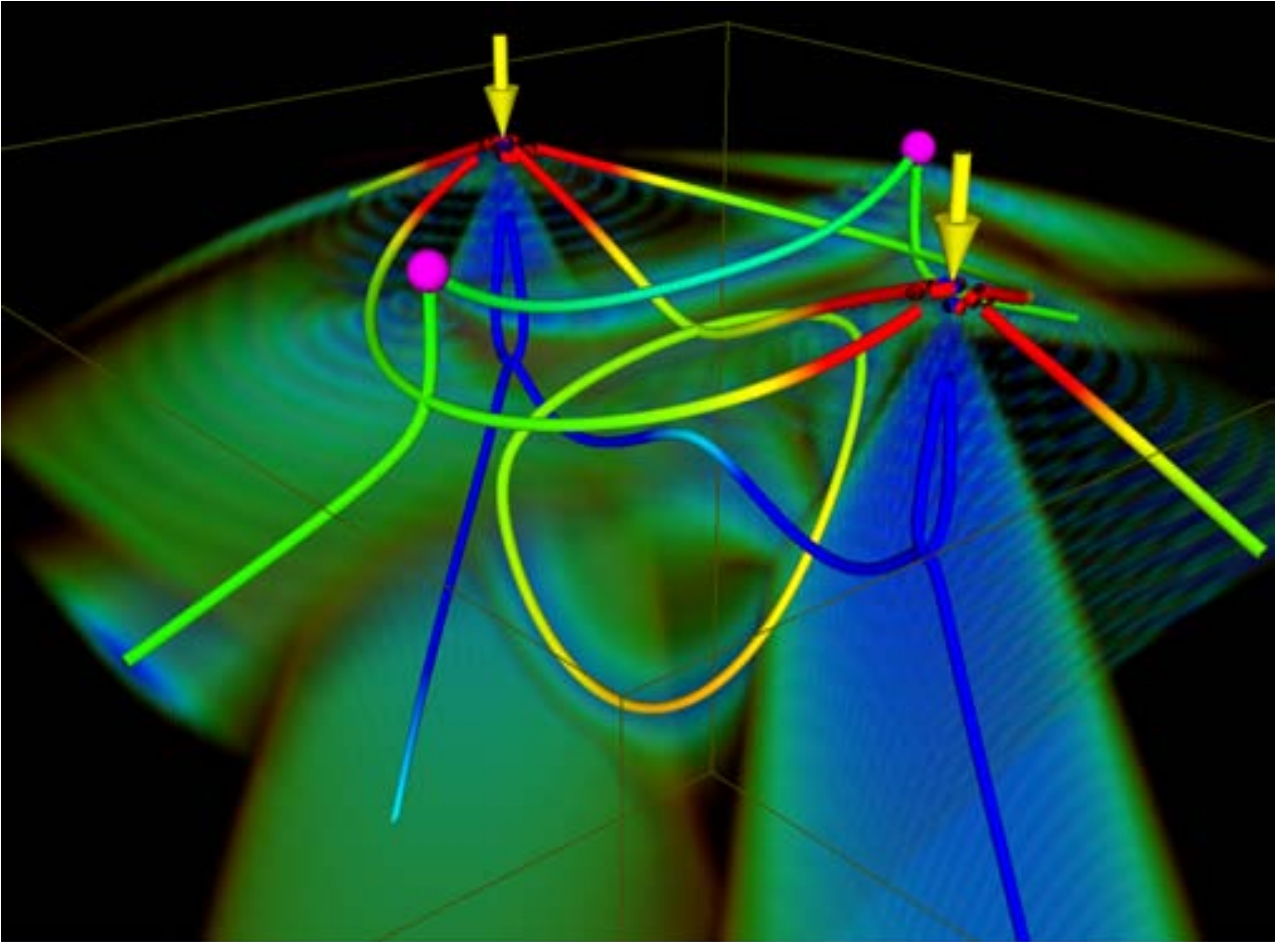
\includegraphics[width=0.6\textwidth]{figures/tensor_topology.png}
    \end{captionbeside}
\end{figure}
%

\subsubsection{Separatrices} % (fold)
%
The tensor field lines that pass through a degenerate point form separatrices
that separate the neighborhood of the point into sectors~\cite{Delmarcelle1994}.
%
These structures are akin to the separatrices of vector fields that separate
the area around a saddle point.
%
In \ac{2D}, these separatrices are lines, in \ac{3D}, they form surfaces.
%
An algorithm for extracting such surfaces from \ac{3D} tensor fields was
proposed by Zheng \etal{}~\cite{Zheng2005b}
%

\subsubsection{Neutral and Traceless Tensors} % (fold)
%
A different kind of topological feature are neutral and traceless tensors,
which were first investigated bu Palacios \etal{}~\cite{Palacios2016}.
%
A neutral tensor is a tensor where the middle eigenvalue is the average of the
major and minor eigenvalue.
%
Neutral tensors in \ac{3D} tensor fields form surfaces.
%
These surfaces mark the transition between areas of linear tensors (one
dominating eigenvalue) and planar tensors (two dominating eigenvalues).
%
In stress tensors, these can be interpreted as the transition between
predominantly tensile stress and predominantly compressive stress.
%
In diffusion tensors from \ac{DTI}, they indicate the separation between
regions with clear fiber direction and regions where fiber tracts cross.
%

%
Traceless tensors are tensors whose sum of eigenvalues is zero.
%
Traceless tensors also form surfaces in \ac{3D} tensor fields.
%
They mark the transition between areas of positive and negative trace.
%
In stress and strain tensors, these are equivalent to regions of expansion and
compression.
%
Recently, Roy \etal{}~\cite{Roy2019} proposed a more robust extraction method for
these surfaces as well as degenerate lines.
%

\subsubsection{Topology of General (Asymmetric) Tensor Fields} % (fold)
%
The topology of general tensor fields has been studied to a lesser extent.
%
Zheng and Pang~\cite{Zheng2005a} first introduced \emph{circular points} as the
main topological structure in \ac{2D} general tensor fields.
%
These are points where the tensor is a perfect rotation matrix.
%
Analogous to degenerate points in symmetric tensor fields, these are also points
where all vectors are valid eigenvectors.
%
Degenerate structures where two eigenvalues are equal also exist in general
tensor fields, but here they mark the transition between regions of real and
complex eigenvectors.
%
This means that they form lines instead of points in \ac{2D}, and their meaning
is very different.
%
Zhang \etal{}~\cite{Zhang2009} later extended the study of \ac{2D} general tensor
fields by defining eigenvector and eigenvalue manifolds to classify general
tensors and distinguish different types of circular points.
%
% subsection topological_methods (end)
%
% section tensor_fields (end)
%
% chapter sci_vis (end)
%
\chapter{Introduction to Turbulent Combustion} % (fold)
\label{cha:turbulent_combustion}
%
\lettrine[lines=3, findent=-2pt, nindent=2pt, lhang=0.05]{C}{ombustion} is one
of the cornerstones of our civilization.
%
It provides light in a candle or carries objects into space in a rocket engine.
%
The majority of high-tech combustion processes occur under turbulent conditions.
%
The nature of turbulent flow, and therefore also turbulent combustion, is still
being actively studied by the scientific community.
%
Reducing the pollutant emissions and increasing the efficiency of combustion
processes is essential in todays world where we are confronted more and more
often with the realization that our resources are finite and the damage we do to
our environment can not easily be undone.
%

%
Simulations are an invaluable tool in the design of improved combustion
processes.
%
They allow to test different setups quickly and for a relatively low cost.
%
Efficient simulations need models of the relevant physical and chemical
processes.
%
As the demands on the accuracy of such models rises, more detailed insight into
the low-level phenomena of turbulent combustion is needed.
%
Obtaining this insight via experiments is challenging.
%
Often only a small number of variables can be observed at the same time and
observations are frequently limited to a \ac{2D} slice.
%

%
Another approach is \acf{DNS}, which is sometimes referred to as a ``numerical
experiment''.
%
In \ac{DNS}, the Navier-Stokes equation is directly solved on a very fine grid,
without using any higher-level modeling assumptions.
%
This is computationally very expensive, which is why \ac{DNS} is typically
performed on supercomputers using hundreds or thousands of cores.
%
In the simulation, all variables are available in full spatial and temporal
resolution.
%

%
Analyzing the data from such simulations poses a different challenge.
%
Due to the high spatial and temporal resolution, the raw data produced by a
single \ac{DNS} run can range from Terabytes to Petabytes.
%
Data of this size can not be written to disk or transferred over a network in a
reasonable amount of time, even if the enormous storage space that is required
was available.
%
This limits the post-analysis of the data to spatially or temporally downsampled
versions which lose a lot of important information.
%
In recent years, the subject of \emph{in-situ} analysis and visualization has
therefore gained popularity.
%
The idea is to process the data while it is still in memory during the
simulation.
%
The raw data is then discarded and only the results, which are typically much
smaller in size, are stored on disk.
%

%
This thesis contains two new in-situ focused approaches for analysis and
visualization of turbulent combustion \ac{DNS}.
%
To provide some important context, this chapter provides a short introduction
into the field of turbulent combustion research, the basics of turbulent
combustion modeling and simulation, and an overview of relevant research
concerning in-situ and post-processing of turbulent combustion data in
particular and large-scale simulations in general.
%
%
\section{Combustion} % (fold)
\label{sec:combustion}
%
Combustion is the exothermic chemical reaction of a fuel and an oxidizer into
oxidized products and heat.
%
We will only concern ourselves with the combustion of gases, which is the
most common case used in industrial applications.
%
The oxidizer is usually oxygen, while fuels can range from simple ones such as
hydrogen or methane to complex organic fuels.
%

%
A combustion process is a complex system of elementary chemical reactions
transforming various chemical species into each other while absorbing or
releasing heat.
%
It involves reactants and products but also various intermediate species.
%
These intermediates can be more or less stable and are often radicals with
unpaired electrons.
%
The reaction rate of each elementary reaction in an infinitesimal volume is
dependent on the amounts (\ie, mass) of the different chemical species as well
as the current temperature.
\Todo{define mass fractions and density}
%
The process can additionally be influenced by the diluting presence of inert
gases that do not participate in the reaction.
%

%
The chemical reactions in a flame are intrinsically linked to the fluid motion
of the gas.
%
As the gas is deformed and transported by the flow, the local concentration and
temperature gradients change, which in turn control the diffusion of chemical
species and heat.
%
Through diffusion, the local mixture and temperature changes, which in turn
influences the reaction rates.
%
As the chemical reactions produce or consume heat, the gas expands or contracts,
which in turn influences the fluid's velocity (the expanded gas has to go
somewhere) and viscosity (molecules that are farther away from each other
interact less).
%
This again influences the mixing and transport of the gas, and so the cycle goes
on.
%

%
Gaseous combustion can be classified by the type of flow and the mixing of
reactants.
%
Is the flow laminar or turbulent, and are fuel and oxidizer premixed or
non-premixed?
%
We will discuss the characteristics of flames in each of these regimes in the
following sections.
%
This discussion is largely based on the book ``Theoretical and Numerical
Combustion'' by Poinsot and Veynante~\cite{Poinsot2012}.
%
\subsection{Laminar Flames} % (fold)
\label{sub:laminar_flames}
%
If the reacting gases in a flame move at low velocities, the flow is often
laminar.
%
Laminar flow is characterized by the absence of eddies or vortices.
%
Layers of the fluid slide past each other without significant mixing.
%
In many cases, the flow is steady in this regime.
%

%
Even though laminar flames are the exception in industrial applications, their
simplicity and deterministic behavior makes them an ideal basis for the
theoretical study of combustion processes.
%
They are the reference case that turbulent combustion is compared against and
that turbulent combustion models are derived from.
%
\subsubsection{Laminar Premixed Flames} % (fold)
\label{ssub:laminar_premixed_flames}
%
In a premixed flame, fuel and oxidizer are brought into a uniform mixture before
ignition.
%
The defining feature of premixed combustion is the flame front that propagates
into the fresh gases and leaves behind hot combustion products.
%
In the simplest case, the flame front is planar and travels along its normal
direction.
%
In this case, the phenomenon is essentially one-dimensional (see
\cref{fig:premixed_profiles}).
%
\begin{figure}[t]
    \centering
    % \MissingFigure{\ac{1D} profiles of an ideal premixed flame}
    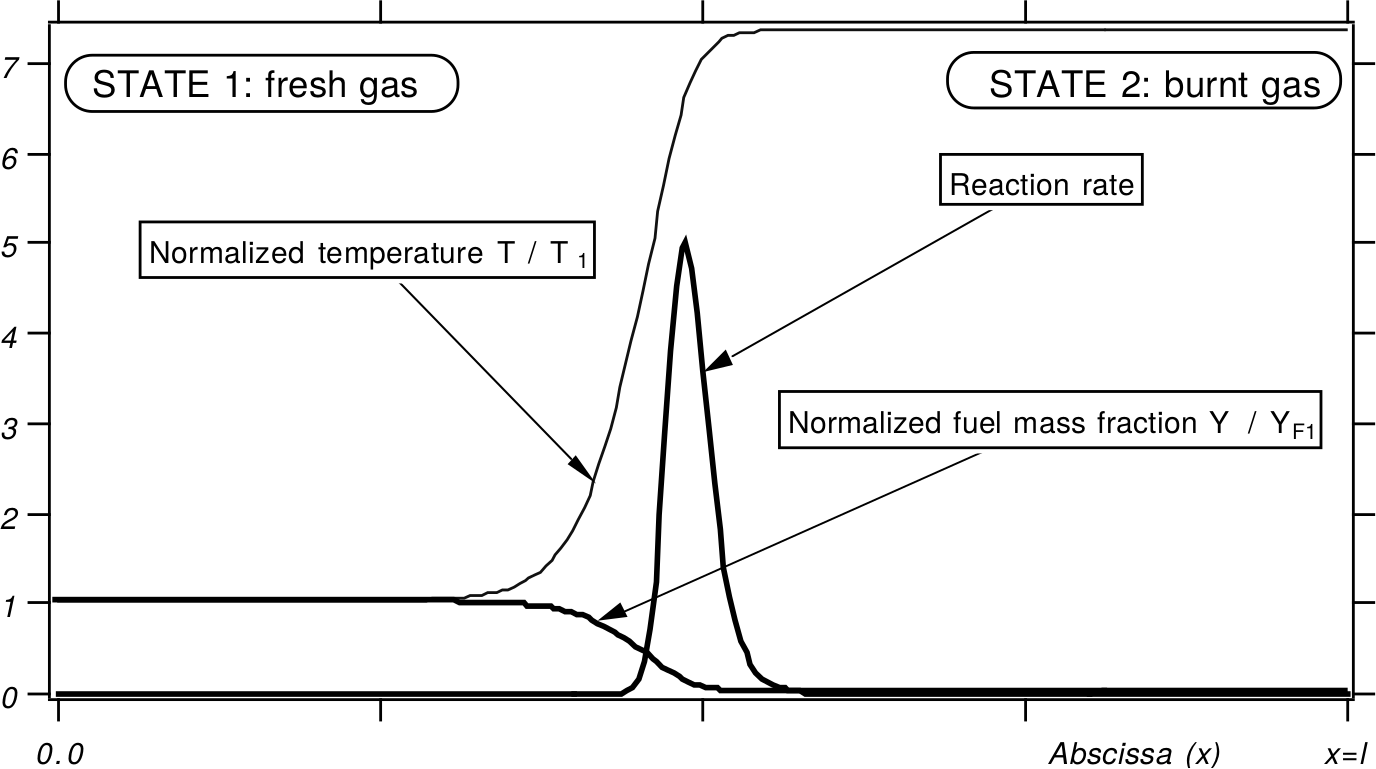
\includegraphics[width=\textwidth]{figures/1D_premixed_flame.png}
    \caption{Basic configuration of a one-dimensional laminar premixed flame.
    Image source: Poinsot and Veynante~\cite{Poinsot2012}}
    \label{fig:premixed_profiles}
\end{figure}
%
The profiles of the combustion variables along the normal direction show high
concentrations of fuel and oxidizer on the fresh gas side and high combustion
product concentrations and temperature on the burnt gas side.
%
In between the two extrema is the flame front that shows the gradual transition
between fresh and burnt gases.
%
The concentration of intermediate species is highest in the flame front.
%
Intermediates generally do not occur in the fresh gases, but some radicals may
exist on the burnt gas side due to dissociation of combustion products at high
temperatures.
%
\begin{figure}[t]
    \centering
    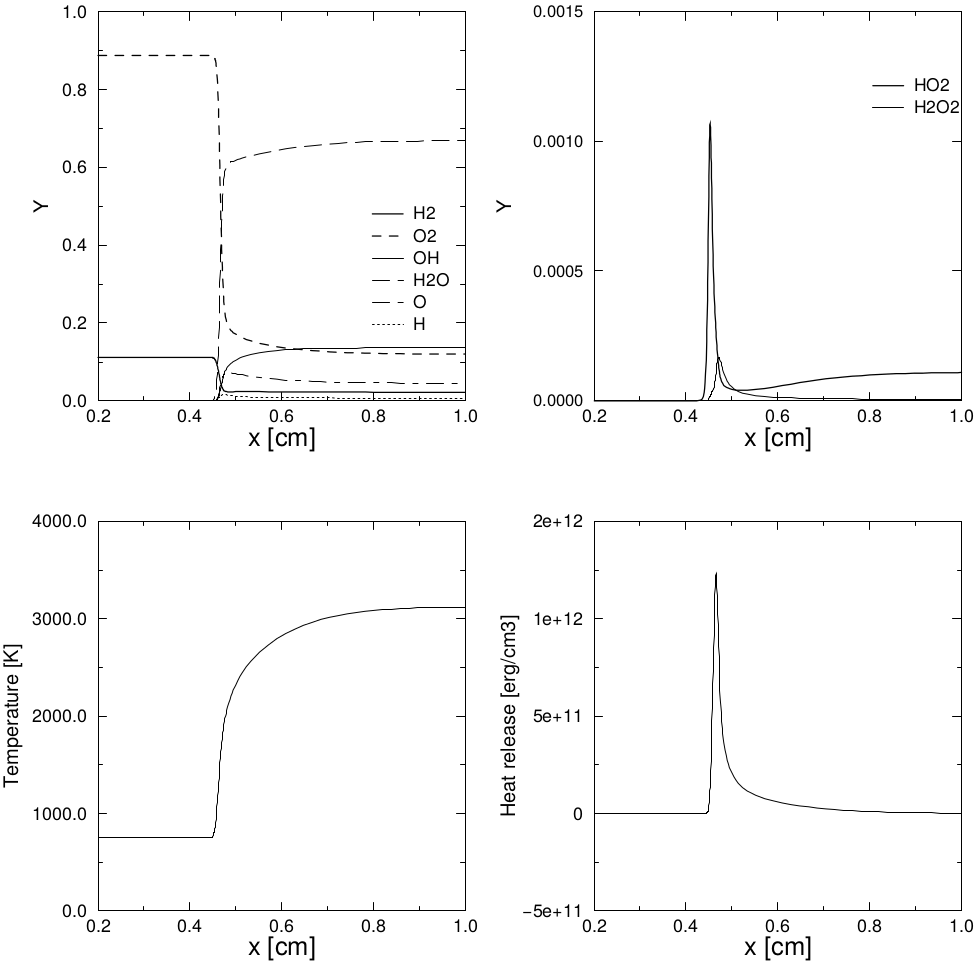
\includegraphics[width=\textwidth]{figures/laminar_flame.png}
    \caption{Profiles of species (Y), temperature and heat release of a
    laminar premixed \ce{H2}-\ce{O2} flame. Image source: Poinsot and
    Veynante~\cite{Poinsot2012}}
    \label{fig:laminar_premixed_profiles}
\end{figure}

%
The characteristic properties of a premixed flame front are \emph{flame speed},
\emph{flame stretch}, and \emph{flame thickness}.
%
These three quantities depend on each other and the underlying flow field.
%

%
The flame speed is the speed at which the flame front travels.
%
It can be expressed relative to a laboratory frame of reference, or relative to
the flow. \Todo{mention in surface tracking chapter which definition is used}
%
Sometimes, it is also expressed as the speed at which fresh gases are turned
into combustion products.
%
The flame speed can vary considerably along the surface of a flame, and
depending on conditions, the flame front can travel against the flow at
considerable speeds.
%

%
The flame thickness describes the width of the reaction zone normal to the flame
front.
%
Depending on the application, it is determined in different ways.
%
One common definition uses the slope at the point of highest temperature
gradient.
%
Another one is based on the distance between the isosurfaces of minimum and
maximum temperature.
%
Different alternative definitions exist as well, some of them based on radical
species.
%
The flame thickness is inversely proportional to the flame speed in canonical
configurations.
%
A thinner flame travels more quickly and slow-moving flames tend to be thicker.
%
Flame thickness is an essential measurement for combustion simulations, as it
determines the grid resolution necessary to resolve the flame front.
%

%
Both flame speed and flame thickness are dependent on the chemical reaction
taking place and the stretch of the flame front.
%
Flame stretch is the change in surface area an infinitesimal element of the
(idealized) flame surface experiences over an infinitesimal time interval.
%
It can be induced by a non-uniform flow, but also by the expansion or
contraction a curved flame front experiences due to its propagation in normal
direction.
%
\Cref{fig:stretched_premixed_flames} shows some examples of stretched laminar
premixed flames.
%
If the flame experiences positive stretch, it is tangentially expanded and
compressed in normal direction.
%
This decreases the flame thickness and feeds new fresh gases to the reaction,
which increases the flame speed.
%
However, it also increases heat dissipation.
%
If the flame is stretched too quickly, this can lead to quenching.
%
Negative stretch (compression) leads to less fresh gas being transported near
the reaction zone, which increases the flame thickness and reduces flame speed.
%
\begin{figure}[tp]
    \centering
    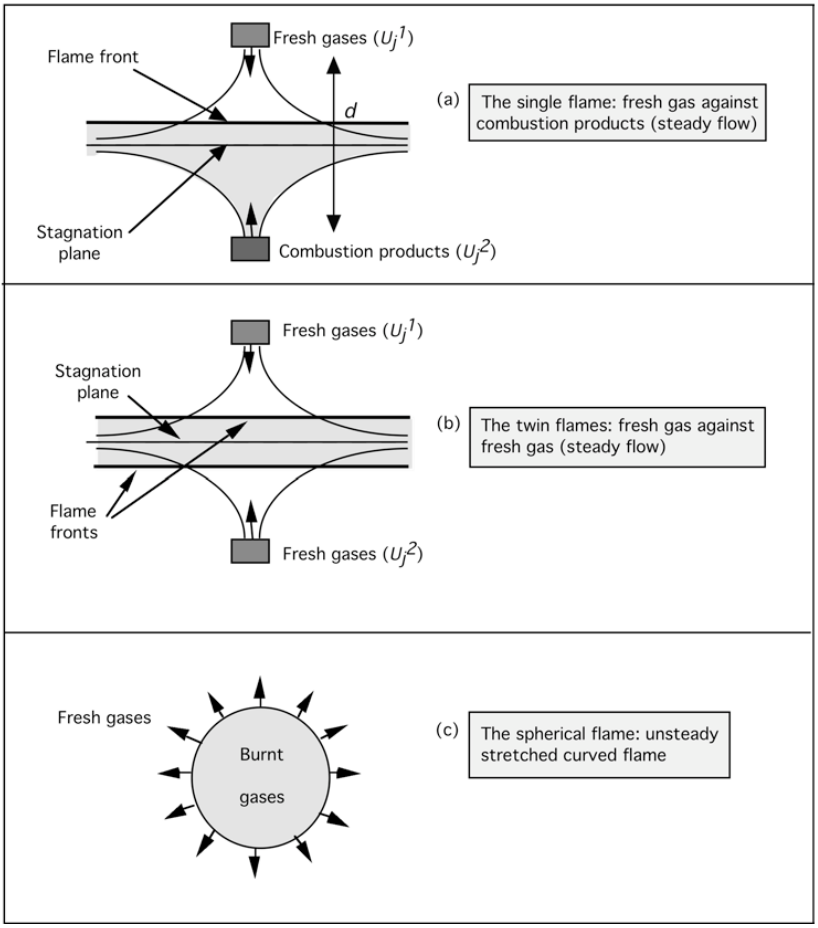
\includegraphics[width=\textwidth]{figures/stretched_premixed_flames.png}
    \caption{Examples of stretched laminar premixed flames. Image source:
    Poinsot and Veynante~\cite{Poinsot2012}}
    \label{fig:stretched_premixed_flames}
\end{figure}

%
Due to their defining characteristic for the behavior of the flame, flame speed,
thickness and stretch are the basis for a lot of combustion models, and a focus
of study in many combustion experiments and simulations.
%
% subsubsection laminar_premixed_flames (end)
%
\subsubsection{Laminar Non-Premixed (Diffusion) Flames} % (fold)
\label{ssub:laminar_diffusion_flames}
%
In non-premixed combustion, fuel and oxidizer are supplied separately.
%
Combustion can only occur where both mix in a sufficient ratio via diffusion.
%
This is why non-premixed flames are also called diffusion flames.
%
\Cref{fig:laminar_diffusion_profiles} shows a \ac{1D} cross-section of a
typical laminar diffusion flame.
%
\begin{figure}[t]
    \centering
    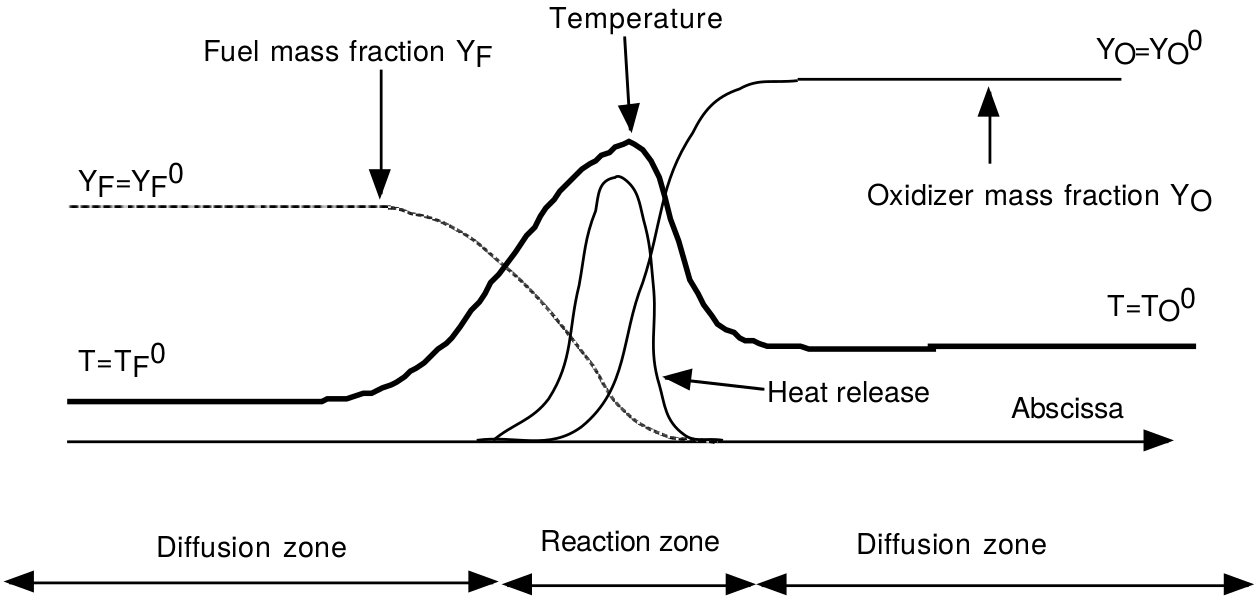
\includegraphics[width=\textwidth]{figures/laminar_diffusion_flame.png}
    \caption{Basic configuration of a one-dimensional laminar diffusion flame.
    Image source: Poinsot and Veynante~\cite{Poinsot2012}}
    \label{fig:laminar_diffusion_profiles}
\end{figure}
%

%
The prototypical example of a diffusion flame is a jet flame where fuel gas is
injected into ambient air and ignited.
%
An example of this type we are all familiar with is the flame of a candle.
%
Wax is evaporated from the wick via the heat of the flame.
%
This fuel gas burns as it comes into contact with ambient air and creates a
laminar diffusion flame.
%
The heat generated from the flame is sufficient to ignite the fresh fuel being
supplied from the wick and sustain the reaction.
%
\Cref{fig:laminar_diffusion_jet} shows a simplified example of such a flame.
%
\begin{figure}[t]
    \centering
    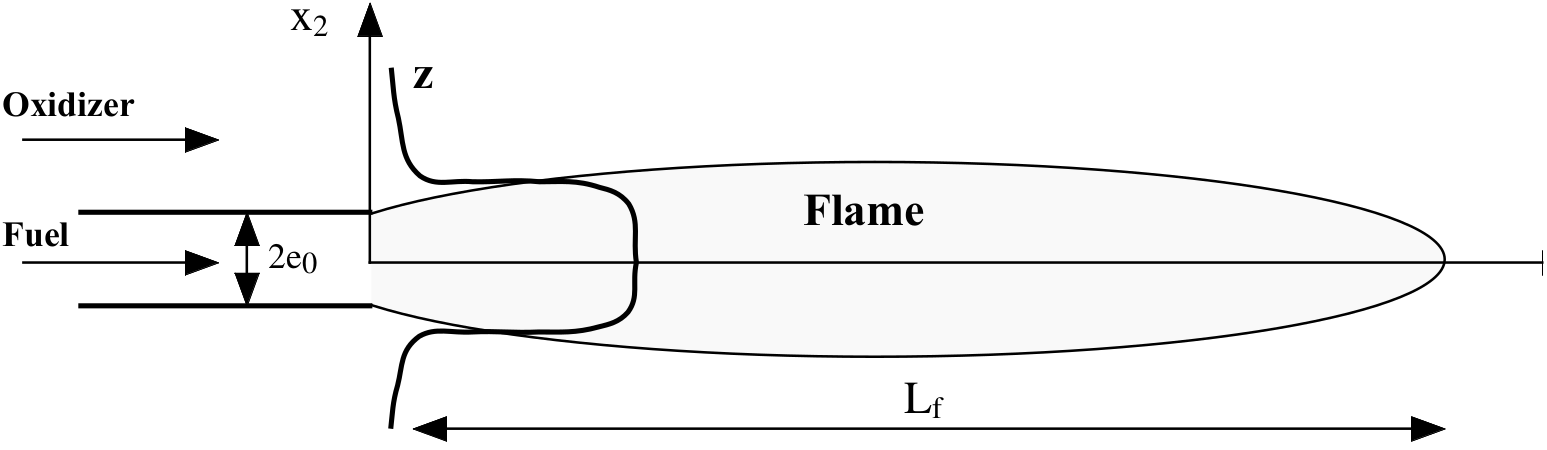
\includegraphics[width=0.8\textwidth]{figures/laminar_diffusion_jet.png}
    \caption{Simple \ac{2D} laminar diffusion jet flame. Image source: Poinsot
    and Veynante~\cite{Poinsot2012}}
    \label{fig:laminar_diffusion_jet}
\end{figure}
%

%
Diffusion flames are easier to set up than premixed flames from a practical
perspective, as no perfect mixing of fuel and oxidizer is required beforehand.
%
They are also safer because they prevent flashbacks into the gas supply.
%
However, it is harder to ensure a clean and complete consumption of fuel in
non-premixed combustion.
%
This is why diffusion flames are generally less efficient and produce more
soot and pollutants that result from suboptimal burning conditions.
%

%
As the conditions for combustion are not satisfied initially, transport and
mixing become the main issues in a non-premixed flame.
%
Fuel and oxidizer need to mix sufficiently to create a combustible mixture.
%
Temperature produced by nearby combustion needs to be high enough to ignite
the mixture.
%
Combustion products need to be transported away from the combustion zone fast
enough to prevent the flame from suffocating, but not too fast to dissipate the
heat required for continued combustion.
%

%
Diffusion flames do not propagate like premixed flames.
%
Their position is fixed at the interface between fuel and oxidizer.
%
For this reason, the speed of the flame is not a relevant quantity for
analyzing the behavior of diffusion flames.
%
Instead, the defining variable is the mixture fraction between fuel and
oxidizer.
%
The flame is generally strongest where the mixture fraction is near
stoichiometry, \ie, where fuel and oxidizer are mixed in such a ratio that
both are consumed completely by the reaction.
%
Mixture fraction and temperature are the dominating variables controlling a
diffusion flame, which is why simple combustion models are based on these two
quantities.
%

%
Unlike for premixed flames, where it mainly influences the speed of the reaction
and can only quench the flame in extreme cases, diffusion flames are very
sensitive to flame stretch.
%
A certain stretch is necessary to supply fresh gases to the reaction zone and
transport away combustion products that would otherwise suffocate the flame.
%
However, for high flame stretch heat might be dissipated too quickly to sustain
the reaction, leading to extinction.
%

%
Because diffusion flames are much more sensitive to the flow conditions, and
combustion occurs over a wider range of fuel/oxidizer mixture fractions,
modeling and simulating diffusion flames is more challenging than premixed
flames.
%
% subsubsection laminar_diffusion_flames (end)
%
% subsection laminar_flames (end)
%
\subsection{Turbulent Flames} % (fold)
\label{sub:turbulent_flames}
%
Although laminar flames are the basis for the study of combustion, most
industrial combustion applications are turbulent in nature.
%
This makes turbulent combustion an important area of research.
%
Unfortunately, it is also a particularly challenging one.
%
Turbulent flow itself is still not well understood by the scientific community,
and understanding and modeling complex chemical reactions still poses a
significant challenge.
%
In turbulent combustion, both of these phenomena are combined and interact with
each other, which makes understanding even more difficult.
%

%
Turbulent flow is a chaotic and essentially statistical process.
%
It occurs when the inertial force of the flow is dominant over the damping
effect caused by the fluid's viscosity.
%
This happens at higher fluid velocities, where small imperfections lead to
disturbances that are not immediately absorbed by viscous effects.
%

%
Turbulent flow is characterized by a mixture of \emph{eddies} of different sizes
and energies.
%
The sizes of eddies in a flow range from the integral length scale, that is
roughly equivalent to the size of the domain the flow resides in, to the
Kolmogorov length scale, that describes the smallest eddies in the system.
%
The energy in a turbulent flow passes along the turbulent spectrum from the
largest length scales to the smallest ones.
%
Large eddies spin off smaller eddies, which spin off even smaller eddies and so
on until the energy is dissipated as heat at the Kolmogorov scale.
%
This is why turbulent flow will decay over time if it is not continuously
supplied with energy.
%

%
The interaction between flow and chemistry in a turbulent flame is a two-way
street.
%
The reaction transforms and heats the gas, changing its density and viscosity
and thereby influencing the flow.
%
On the other hand turbulent flow transports and mixes the gases, thereby
influencing the conditions for combustion.
%
\begin{figure}[t]
    \centering
    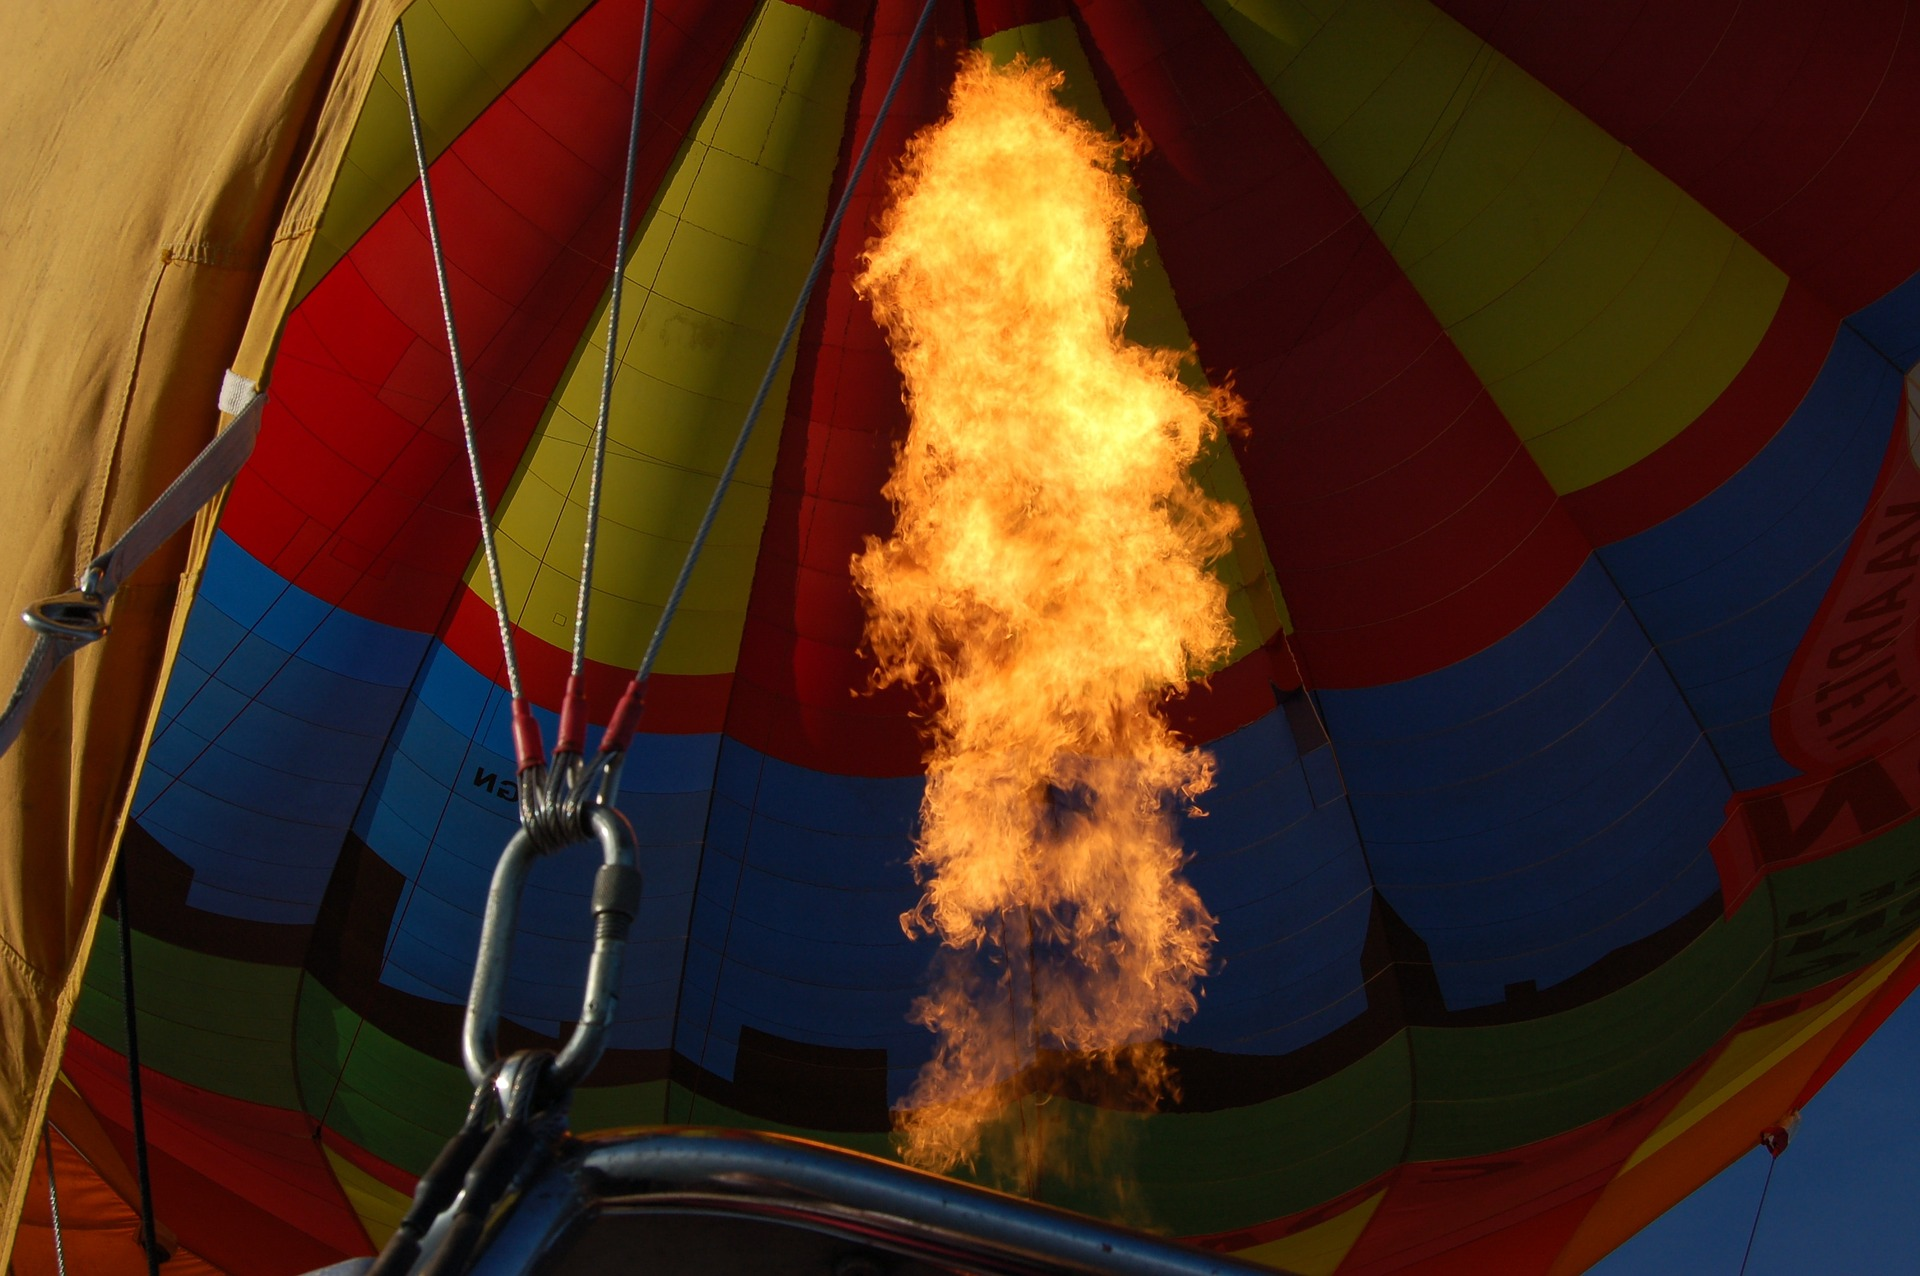
\includegraphics[width=\textwidth]{figures/balloon_burner.jpg}
    \caption{Example of a turbulent non-premixed flame: The burner of a hot air
    balloon.}
    \label{fig:balloon_burner}
\end{figure}
%

%
The effect of turbulence on the flame depends on the size and strength of
the eddies comprising the flow.
%
Large eddies move slowly and only wrinkle the surface in large scales.
%
This only has an indirect effect on the structure of the flame and the chemical
reactions, but influences the global flame shape.
%
Smaller eddies are faster and might disturb the structure of the flame locally.
%
This might have the effect of destroying a clean flame front and causing local
extinction, or it might enhance local mixing and improve the conditions for
combustion.
%
If the eddies are too small, they might be dissipated before they are able to
influence the reaction significantly.
%
Which scales interact with the flame in which way is also dependent on the speed
at which the chemical reaction happens, the flame thickness, and in the case of
premixed combustion, the flame speed.
%
Building accurate models for turbulent combustion requires in\-ves\-ti\-ga\-ting
the interplay of all these variables and more.
%
\subsubsection{Turbulent Premixed Flames} % (fold)
\label{ssub:turbulent_premixed_flames}
%
In premixed flames, turbulence has the primary effect of enhancing combustion.
%
The turbulent flow wrinkles the flame surface and increases its surface area.
%
A higher surface area means that reaction happens at more places at once.
%
The global flame speed increases and fresh gases are consumed more rapidly.
%
However, at high turbulence intensities, the heat produced by the reaction
will be dissipated too quickly and the flame might be extinguished.
%

%
Due to the massive change in viscosity on the burnt gas side, the turbulence
intensity in premixed flames is typically much stronger in the fresh gases.
%
This difference is so significant that the flow on the burnt gas side may become
laminarized, depending on the initial turbulence intensity.
%

%
In practice, premixed combustion occurs for example in spark-ignited internal
combustion engines.
%
Here, air-fuel mixture is sucked into the cylinder, compressed and then ignited.
%
Starting from the ignition point, the flame front travels through the cylinder,
being wrinkled by the turbulent flow of the gas and transforming fresh gases
into hot combustion products.
%
% subsubsection turbulent_premixed_flames (end)
%
\subsubsection{Turbulent Diffusion Flames} % (fold)
\label{ssub:turbulent_diffusion_flames}
%
The typical diffusion flame setup is the jet flame.
%
A stream of fuel gas, often turbulent, is injected into ambient air.
%
Mixing between fuel and air is provided by the turbulent shear layer that arises
from the difference in velocities between the two gases.
%
This leads to a reaction zone that is typically very thin at the outlet and
becomes thicker as more mixing occurs downstream, where a substantial volume is
occupied by combustion products.
%
A practical example for a diffusion jet flame is shown in
\cref{fig:balloon_burner}.
%

%
A central problem of turbulent diffusion flames is flame stabilization.
%
Typically, combustion does not start directly after the fuel gas leaves the
inlet, but only after some mixing has occurred.
%
This mixed gas then needs to be ignited by already-burning mixture further
downstream.
%
This lateral propagation of the flame needs to happen at least at the same
velocity as the flow, otherwise the flame will be blown off.
%
To make this process more stable, some setups provide small premixed pilot
flames between fuel an air stream to provide a steady source of heat.
%

%
If mixing occurs faster than combustion, or if the flame is locally extinguished
due to high flame stretch, pockets of premixed gas can form that are later
ignited when coming into contact with high-temperature regions.
%
This means that parts of a diffusion flame might actually be in the premixed
regime.
%
This highlights the complexity of diffusion flames compared to premixed flames.
%
Due to the additional problem of mixing, diffusion flames are much more
sensitive to turbulence.
%
Depending on their setup, many different conditions and mechanisms can be in
effect at the same time.
%
This makes non-premixed flames very challenging to model and simulate.
%
% subsubsection turbulent_diffusion_flames (end)
%
% subsection turbulent_combustion (end)
%
% section combustion (end)
%
\section{Modeling and Simulation of Turbulent Combustion} % (fold)
\label{sec:simulation_of_turbulent_combustion}
%
Simulations are used to make predictions about the behavior of a system.
%
In turbulent combustion and other engineering application they provide a
quick and cheap way of testing setups compared to setting up experiments.
%
A simulation is only useful if it is sufficiently accurate.
%
This is why good models of the underlying processes are so important.
%
On the other hand, simulations also need to be efficient.
%
If running the simulation is more expensive and time-consuming than setting up
a comparable experiment, the simulation loses its value.
%

%
For turbulent combustion, finding a good trade-off between accuracy and
efficiency is very much an open problem.
%
Both turbulent flow and chemical reactions are complex to model and expensive
to simulate on their own.
%
Solving both at once in a turbulent combustion simulation predictably leads to
a vast increase in the required computing time and resources.
%
Frequently simplifying assumptions are made to gain efficiency.
%
Which assumptions are valid under which circumstances is the central question
when building turbulent combustion models.
%

%
This section provides an overview of modeling strategies used in turbulent
combustion simulations.
%
It places a particular focus on \acl{DNS}, as it is most relevant for the
content of this thesis.
%
\subsection{Chemical Schemes} % (fold)
\label{sub:chemical_schemes}
%
Modeling a chemical reaction can be a complex task.
%
Most reactions do not consist of a single step but rather a complex system of
intermediate reactions.
%
Many of these reactions can be reversible and their reaction rates depend on the
current composition and pressure or temperature of the gas.
%
The more complex the fuel, the more intermediate steps are possible and need to
be considered when modeling the reaction.
%
A system of intermediate steps that models a whole reaction is called a chemical
scheme (see, \eg, \cref{tab:hydrogen_scheme}).
%
Each individual reaction step has a number of parameters controlling the
reaction rate in dependence on the current conditions.
%
\begin{table}[t]
    \caption[Example scheme for \ce{H2}-\ce{O2} combustion]
            {Example scheme for a seemingly simple chemical reaction: hydrogen
             and oxygen react to produce water \cite{Miller1982}. \ce{M} is a
             placeholder for any third molecule that is needed to absorb and
             dissipate excess energy to stabilize the product.}
    \label{tab:hydrogen_scheme}
    \centering
    \begin{tabularx}{\linewidth}{lX}
    \toprule
    \textbf{Elements:} & \ce{H},  \ce{O},  \ce{N} \\
    \midrule
    \textbf{Species:} & \ce{H2}, \ce{O2}, \ce{OH}, \ce{O}, \ce{H}, \ce{H2O},
                        \ce{HO2}, \ce{H2O2}, \ce{N2}\\
    \midrule
    \textbf{Reactions:} &
    {$\begin{aligned}
        \ce{H2 + O2 &<=> 2 OH} & \ce{2 OH &<=> O + H2O}\\
        \ce{H2 + OH &<=> H2O + H} & \ce{H2 + M &<=> 2 H + M}\\
        \ce{H + O2 &<=> OH + O} & \ce{O2 + M &<=> 2 O + M}\\
        \ce{O + H2 &<=> OH + H} & \ce{H + OH + M &<=> H2O + M}\\
        \ce{H + O2 + M &<=> HO2 + M} & \ce{HO2 + H &<=> H2 + O2}\\
        \ce{H + 2 O2 &<=> HO2 + O2} & \ce{2 HO2 &<=> H2O2 + O2}\\
        \ce{H + O2 + N2 &<=> HO2 + N2} & \ce{H2O2 + M &<=> 2 OH + M}\\
        \ce{OH + HO2 &<=> H2O + O2} & \ce{H2O2 + H &<=> H2 + HO2}\\
        \ce{H + HO2 &<=> 2 OH} & \ce{H2O2 + OH &<=> H2O + HO2}\\
        \ce{O + HO2 &<=> O2 + OH} &
    \end{aligned}$}\\
    \bottomrule
    \end{tabularx}
\end{table}
%

%
Reaction modeling is the task of breaking down the wealth of possible
intermediate reactions into a subset that describes the whole reaction with
sufficient accuracy for a given application, and determining the right
parameters for each one.
%
For complex hydrocarbon fuels the number of different species considered
can easily go into the hundreds, while thousands of intermediate steps
contribute to the reaction.
%
Even for seemingly simple reactions, such as hydrogen and oxygen to water,
the reaction schemes can be surprisingly complex.
%
The scheme by Miller \etal~\cite{Miller1982} displayed in
\cref{tab:hydrogen_scheme} has 9 species and 19 different reversible reactions.
%
Adding this to an already computationally intensive fluid dynamics simulation
that only involves five different variables (density, temperature and three
velocity components) increases the computational load immensely.
%
This is amplified even more by the fact that chemical reactions, especially the
intermediate ones in a reaction scheme, typically happen at much smaller time
scales than the flow.
%
This means that compared to non-reacting flows, not only do the number of
equations and variables increase immensely, but the simulation time steps also
become much smaller.
%

%
There are some strategies to increase efficiency.
%
The simplest one is to use single-step chemistry.
%
Here, the reaction is assumed to be infinitely fast and the flame front to be
infinitely thin.
%
Fuel and oxidizer are immediately transformed into products and heat once the
conditions for combustion are met.
%
In this case, no intermediate reactions are considered, which greatly decreases
the number of variables and equations to solve and allows larger time steps.
%
Due to the strong assumptions made when using this method, the results can be
very inaccurate, but it can be useful to get a qualitative result.
%
More accurate but also more expensive methods precompute a lookup table covering
the relevant portion of the parameter space or reduce the parameter space to
lower-dimensional manifolds.
%
Explaining these methods in detail is out of the scope of this work.
%

%
Modeling chemical reactions is a complex field in its own right.
%
Turbulent combustion researchers mostly use existing chemical libraries and
schemes in their codes.
%
Often, the trade-off between accuracy and efficiency has to lean heavily towards
efficiency to keep simulation times and memory usage in a reasonable range.
%
% subsection chemical_schemes (end)
%
\subsection{The Flamelet Assumption} % (fold)
\label{sub:the_flamelet_assumption}
%
Moving from reactions to turbulent flames, we need a model for the structure
of the flame.
%
The most common assumption is that the flame front is thin compared to the
scales of the turbulent eddies.
%
This means that the flame front can be approximated by an isosurface of the
reaction progress variable in the case of premixed flames or the mixture
fraction for diffusion flames.
%
Assuming a thin flame front allows to treat the turbulent flame like a set of
locally laminar flames, so-called \emph{flamelets}, that are wrinkled but not
disturbed by the flow.
%
Orthogonal to the surface, the flame is assumed to behave like the
\ac{1D} laminar equivalent.
%
Models for laminar combustion can then be directly used to determine the
behavior of the flame at each location on the idealized flame surface.
%
This includes models for the relationship between flame speed, flame stretch,
flame thickness, reaction rates, heat release and so on.
%

%
The flamelet assumption is frequent in combustion modeling, as it greatly
simplifies the flame structure and limits the effects of turbulence on the
behavior of the flame that need to be considered.
%
Of course, the conditions for this assumption are not always fulfilled:
%
\begin{itemize}
    \item
    %
    Parts of the flame might be locally quenched.
    %
    In the case of premixed flames, this allows fresh gases to penetrate into
    the burnt gas side and vice-versa, something that does not happen for
    laminar flames.
    %
    In the case of diffusion flames, this allows the formation of pockets of
    premixed gas that are later ignited and do not confirm to the ideal
    diffusion flame any more.
    %
    \item
    %
    The ideal flame front might be disturbed by small-scale mixing.
    %
    In this case, the flame structure can be very different than that of laminar
    flames.
    %
    The distinction between burnt/unburnt or fuel/oxidizer side becomes less
    clear and the flame structure can no longer be adequately described by a
    simple isosurface.
\end{itemize}
%
Due to the simpler flame structure and the smaller sensitivity to turbulence,
the flamelet assumption is more often valid for premixed than for diffusion
flames.
%
More complex models that allow some interaction of turbulence with the
small-scale flame structure are subject of ongoing research.
%
% subsection the_flamelet_assumption (end)
%
\subsection[High-Level Models: RANS and LES]
           {High-Level Models: \acs{RANS} and \acs{LES}} % (fold)
\label{sub:high_level_models}
%
\begin{figure}[t]
    \centering
    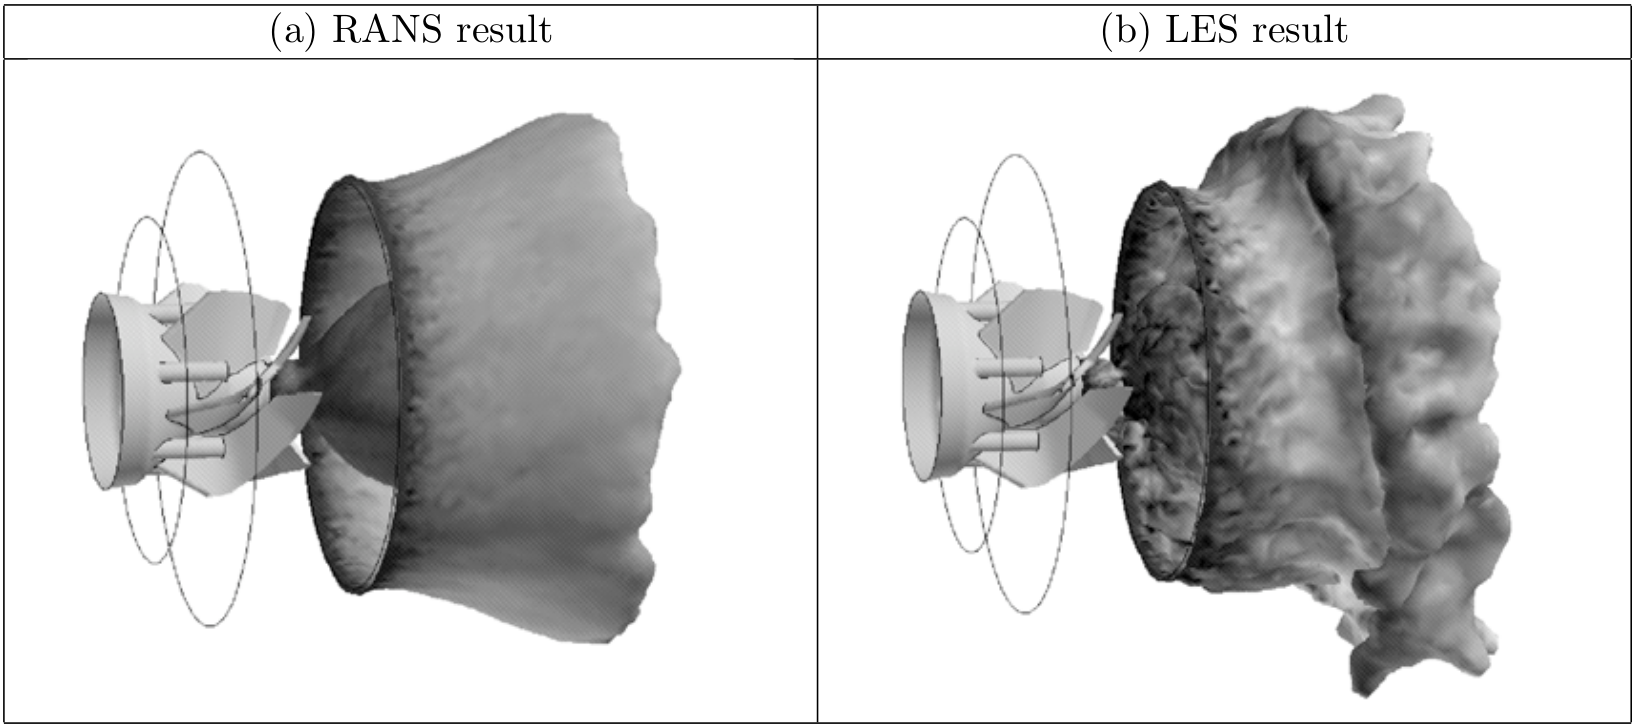
\includegraphics[width=\textwidth]{figures/rans_vs_les.png}
    \caption{Comparison of temperature isosurfaces in a swirled combustor when
    using \ac{RANS} and \ac{LES}. Image source: Poinsot and Veynante
    \cite{Poinsot2012}}
    \label{fig:rans_vs_les}
\end{figure}
%
Computational fluid dynamics (\acs{CFD}\acused{CFD}) knows three main categories
of models for simulating turbulent flow.
%
They are, in decreasing order of abstraction, \acf{RANS}, \acf{LES} and
\acf{DNS}.
%
For simulating turbulent combustion, these are extended by combustion models
according to their character.
%
The first part of this thesis focuses heavily on \ac{DNS}, which is discussed in
detail in the next section.
%
Since \ac{DNS} is one of the main tools for validating and building \ac{RANS}
and \ac{LES} models, we will briefly discuss the ideas behind both here.
%
\subsubsection{Reynolds-Averaged Navier-Stokes} % (fold)
\label{ssub:rans}
%
\acl{RANS} equations describe the time-averaged behavior of the system.
%
It is based on the decomposition of a turbulent flow into mean and
fluctuating parts.
%
The result are average values for all simulation variables at each location.
%
Images of \ac{RANS} simulations show very smooth fields that have almost no
small-scale features (see \eg, \cref{fig:rans_vs_les}).
%
The typical \ac{RANS} equations assume a steady-state system, but the \ac{URANS}
variant can account for some unsteady behavior if it is slow compared to the
turbulent timescales.
%

%
Combustion models for \ac{RANS} can be based on quantities such as the mean
flame surface area per unit volume, turbulent mixing rates, or probability
density functions based on one-point statistics.
%

%
Since \ac{RANS} simulations only resolve time-averaged values, their results
have to be interpreted with care.
%
Mean values reported by \ac{RANS} at a certain location say nothing about the
possibly large fluctuations that occur there.
%
However, \ac{RANS} is the most popular and widespread method for simulating
turbulent combustion because of its low computational cost.
%
% subsubsection rans (end)
%
\subsubsection{Large Eddy Simulations} % (fold)
\label{ssub:les}
%
A step up from \ac{RANS} in terms of accuracy and computational cost are
\ac{LES}.
%
They reproduce unsteady, but low-pass filtered effects of the system.
%
The simulation runs on a lower-resolution grid and only resolves the larger
scales explicitly.
%
Small-scale sub-grid effects are modeled.
%
\ac{LES} produce an unsteady, but "blurry" representation of reality (see
\cref{fig:rans_vs_les}).
%

%
Combustion models for \ac{LES} face the challenge that the flame front is
generally much smaller than the grid resolution.
%
Combustion phenomena that control the evolution of the flame front happen almost
exclusively at sub-grid scales.
%
\ac{LES} approaches deal with this by describing the flame front in terms of
some filtered variable that can be resolved on the grid.
%
Some approaches artificially thicken the flame front, others assume the
flame front as an isosurface of some smooth variable.
%
In any case, small-scale wrinkling of the flame front cannot be resolved in
\ac{LES} and needs to be expressed via models.
%

%
With the increase in computing performance in recent years, \ac{LES} has gained
popularity and is seeing more widespread use.
%
However, \ac{LES} of turbulent combustion is still maturing, and accurate
sub-grid models for combustion are the subject of ongoing research.
%
% subsubsection les (end)
%
% subsection high_level_models_for_turbulent_combustion_ac (end)
%
\subsection{Direct Numerical Simulations} % (fold)
\label{sub:direct_numerical_simulations}
%
The most accurate and detailed numerical results in \ac{CFD} are produced by
\ac{DNS}.
%
In these simulations, all time and length scales are resolved on a regular grid.
%
On this grid, the Navier-Stokes equations are solved directly without using a
model for turbulence.
%
This produces an accurate representation of reality, which is why \ac{DNS} is
also often referred to as a ``numerical experiment''.
%

%
Its brute-force approach means that \ac{DNS} is conceptually relatively simple
compared to \ac{RANS} and \ac{LES}, but it is the most demanding of the three
in terms of computational resources and time.
%
As a consequence, \ac{DNS} are typically used only for small domains of a few
centimeters at most.
%
Although methods for more complex setups and geometries are under active
development, the typical case is a rectangular box with simple boundary
conditions.
%
This is why non-reacting \ac{DNS} has typically been used to study turbulent
flows near walls, between parallel plates or behind simple rectangular
geometries.
%

%
Like for \ac{RANS} and \ac{LES}, the choice of a chemistry model for \ac{DNS} is
largely dependent on the available computing resources and performance demands.
%
If we apply the ideal of solving everything without high-level models, then the
logical choice would be using complex chemistry with full chemical schemes.
%
Unfortunately, this is rarely feasible.
%
Even adding single-step chemistry to a non-reacting \ac{DNS} can result in a
hundred-fold increase in computing time due to the smaller time steps and grid
sizes required.
%
Using complex chemical schemes only amplifies this problem.
%
For complex fuels, the only choice for getting results in a reasonable time
frame is therefore to make a massive trade of accuracy in favor of performance.
%
Even then, turbulent combustion \ac{DNS} of non-trivial cases can only be run
on large supercomputers using thousands of parallel cores.
%
See S3D~\cite{Chen2009,Treichler2017} and DINO~\cite{Abdelsamie2016} for two
modern \ac{DNS} codes.
%

%
Despite the large computational cost and restriction to simple case setups,
\ac{DNS} is an important tool for combustion modeling.
%
It provides high-resolution \ac{3D} unsteady data for all variables, which is
still impossible to obtain via experiments.
%
This data allows an in-depth analysis of the behavior of turbulent flames that
can be leveraged to build, validate and improve higher-level models.
%
\begin{figure}[t]
    \centering
    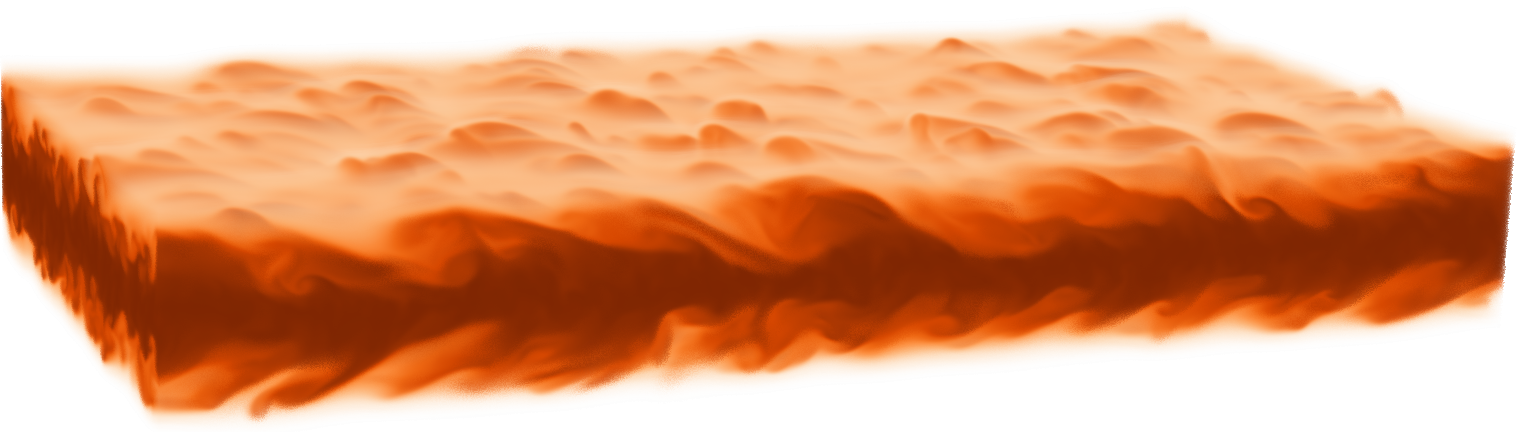
\includegraphics[width=\textwidth]{figures/Hawkes_VolRend.png}
    \caption{Direct volume rendering of the mixture fraction in a
    \ac{DNS} of a turbulent non-premixed flame.}
    \label{fig:turbulent_diffusion_flame_dns}
\end{figure}
%

%
\ac{DNS} is used mainly for two purposes:
%
Gaining data to validate and fine-tune \ac{RANS} and \ac{LES} models, and
gaining a deeper understanding of turbulence/chemistry interactions to derive
new models.
%
A wide variety of analysis approaches are applied to these effects.
%
These range from very simple validation by looking at aggregated quantities to
investigation of complex effects such as the different mechanisms for
re-ignition of locally extinguished parts of the flame.
%
Providing an exhaustive discussion would go beyond the scope of this chapter,
but we will take a look at some examples to get an idea of the kind of
properties that are investigated.
%

%
The simplest forms of analysis are applied for the validation of \ac{RANS} and
\ac{LES} models.
%
Here, the same case is simulated once using \ac{RANS} or \ac{LES}, and once
using \ac{DNS}.
%
Validation can happen at a high level by comparing aggregated quantities such as
the average or maximum temperatures, or on a lower level by comparing point-wise
quantities or statistics.
%
In this case it is important to take into account the differences in
representation between \ac{DNS} and the higher-level models.
%
In the case of \ac{RANS}, \ac{DNS} results have to be temporally averaged in
order to be meaningfully comparable.
%
For \ac{LES}, the \ac{DNS} data needs to be low-pass filtered before comparison.
%

%
More complex analysis is needed when checking the validity of basic assumptions
underlying the high-level models, such as the flamelet assumption.
%
In the case of \ac{RANS}, this can be done by computing different kinds of
statistics, depending on the combustion model used.
%
Simple point statistics can be computed without regard for the flame structure.
%
If the flame front is thin, flamelets may be extracted as profiles orthogonal
to an isosurface representing the flame surface, or along trajectories of the
temperature or mixture fraction gradient.
%
Statistics may also be derived from ensembles of iso-levels of characteristic
variables such as temperature or mixture fraction.
%
The result are distributions as a function of this variable.
%
Finally, space-averaged statistics might be used to determine quantities such as
the average amount of flame surface area per unit volume.
%

%
Other quantities that are often investigated due to their significance in
combustion modeling are the flame speed (if applicable), thickness, surface
stretch and curvature.
%
The relationship of all of these quantities with the structure of the flame is
still not completely understood.
%
This is why \ac{DNS} results are frequently compared to laminar flames as a
baseline.
%
For example, Sankaran \etal \cite{Sankaran2007} analyzed the flame thickness and
curvature in a premixed jet flame statistically and compared the results to a
laminar flame.
%
Hawkes and Chen~\cite{Hawkes2006} investigated the statistical similarity of
methane-air flames in the ``thin reaction zones'' regime, which uses slightly
weaker assumptions than the flamelet regime, to strained laminar flames.
%
The approach presented in \cref{cha:sparse_representation} facilitates such
studies by providing a representation of a premixed flame from which such
statistics can readily be computed, as well as enhancing it by an additional
possibility of visual analysis.
%

%
A promising area of current research is concerned with the mechanisms of local
extinction and re-ignition and the effect of unsteady, non-instantaneous effects
on the flame.
%
These are especially interesting for diffusion flames, as they are more
sensitive to turbulence and local extinction has a major significance for the
applicability of flamelet models.
%
Many works in this area use Lagrangian approaches to study the temporal behavior
of flame elements.
%

%
Yeung \etal \cite{Yeung1990} tracked ensembles of points attached to material-
and flame surfaces in premixed and diffusion flames.
%
They recorded the histories of strain rates acting on these surface points to
determine under what circumstances a flame surface remains close to an initially
coincident material surface.
%
Statistics extracted from the ensemble of surface points allowed them to
determine in what way the flame surface grows or shrinks over time and how the
strain experienced by a flame surface element affects the flame dynamics.
%

%
Sripakagorn \etal \cite{Sripakagorn2004} tracked points attached to an
isosurface of the mixture fraction over time to detect and classify local
extinction and re-ignition events.
%
They showed that extinction happens primarily if the flame surface is subject to
large amounts of strain over a certain time period.
%
They also identified three different mechanisms for re-ignition of previously
extinguished parts of the flame.
%

%
Scholtissek \etal \cite{Scholtissek2017} tracked complete flamelets represented
as trajectories of the mixture fraction gradient emanating from such points on
the mixture fraction isosurface.
%
They analyzed the histories of these flamelets and derived a new flamelet model
that accounts for curvature-induced tangential transport between adjacent
flamelets.
%

%
Such Lagrangian approaches are becoming more prevalent in the combustion
community.
%
They provide an important tool for the derivation of new combustion models
that incorporate unsteady effects.
%
\Cref{cha:flame_surface_tracking} of this thesis presents an approach for
tracking the complete flame surface that is intended to support such
investigations in large-scale \ac{DNS}.
%
% subsection direct_numerical_simulations_for_turbulent_combustion (end)
%
% section modeling_and_simulation_of_turbulent_combustion (end)
%
\section{Visualization for Turbulent Combustion Simulations} % (fold)
\label{sec:visualization_for_turbulent_combustion_simulations}
%
Apart from the mostly statistical forms of analysis that have been traditionally
employed by turbulent combustion researchers, visualization has become an
important tool for gaining understanding from simulation data.
%
Simple visualization techniques such as slicing, isosurface rendering and
scatter plots are routinely used by combustion researchers to gain an overview of
the data.
%
Special techniques for visualization-supported analysis have been developed to
answer more complex research questions.
%
They are essential for understanding the increasingly complex phenomena
incorporated into modern \ac{RANS} and \ac{LES} models.
%

%
As the computing power of supercomputers is steadily increasing, so is the size
and complexity of problems simulated with \ac{DNS}.
%
Storage and network infrastructure are developing at a much slower pace.
%
This has brought us to a situation where the bottleneck in the simulation
pipeline has shifted from the \ac{CPU} to the hard disk.
%
A single snapshot of a \ac{3D} turbulent combustion \ac{DNS} run occupies tens
to hundreds of gigabytes.
%
With thousands of time steps per simulation the raw data produced by a single
simulation can easily reach into the tera- or even petabytes.
%

%
The problem with this is twofold.
%
First, most supercomputers today simply do not have the hard disk space to store
more than a couple of simulation runs completely.
%
Second, writing the raw data to disk after each iteration slows down the
simulation by an order of magnitude or more.
%
As a result, researchers often store only a few snapshots with large temporal
gaps in between.
%
This approach limits the analysis of the data to instantaneous quantities.
%
Unsteady effects become almost impossible to observe and rare events such as
local flame extinction are frequently missed.
%

%
In recent years, in-situ approaches have been established as a way to overcome
this problem.
%
The idea is to process the data in parallel to the simulation while it is still
in memory.
%
Only the results of the visualization/analysis, which are typically orders of
magnitude smaller than the raw data, are then stored to disk.
%
Performing such in-situ processing is challenging because it requires a higher
degree of technical sophistication and often comes with the drawback of reduced
interactivity.
%
However, it can take advantage of all the raw data available during the
simulation and therefore enables a much more detailed analysis.
%

%
This section gives an overview of the state of the art in visualization for
turbulent combustion simulations.
%
We will start with simple and advanced post-processing techniques and then go on
to in-situ approaches specialized to turbulent combustion and general purpose
frameworks for in-situ applications.
%
% Distinction between analysis methods in last section and visualization methods
% not always clear. Visualization methods tend to be designed to be applicable
% to a wider range of questions with a focus on the technical side while works
% from the combustion community tend to focus on the specific question to be
% answered and devise analysis methods ad-hoc without a great focus on
% implementation.
%
\subsection{Post-Processing} % (fold)
\label{sub:post_processing}
%
The classic approach for gaining insight from simulation data is to store it on
a hard disk, possibly transfer it to a dedicated analysis workstation, and then
apply any visualization and analysis methods as a post-process.
%
Often basic visualization techniques are sufficient for most analysis tasks.
%
However, several methods that support specific questions in turbulent combustion
research have been developed.
%
\subsubsection{Basic Visualization} % (fold)
\label{ssub:basic_visualization}
%
\begin{figure}[t]
    \centering
    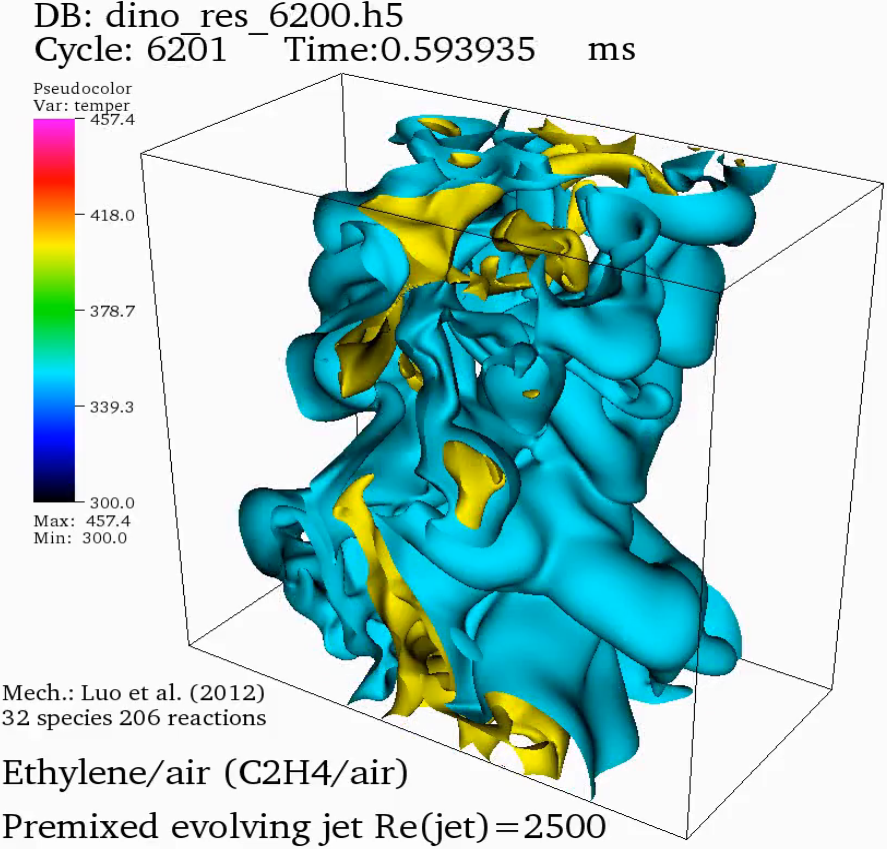
\includegraphics[width=0.8\textwidth]{figures/visit_isosurface.png}
    \caption{Temperature isosurfaces of a premixed jet flame.
        Simulated with DINO~\cite{Abdelsamie2016} and visualized using
        VisIt~\cite{HPV:VisIt}.}
    \label{fig:visit_isosurface}
\end{figure}
%
Combustion researchers have always used simple visualization methods to analyze
their data.
%
Plots of aggregated or point-wise variables over time, space, or other variables
give an idea about the state and behavior of the system.
%
Scatterplots reveal correlations and probability density functions that are the
basis for modeling turbulent combustion phenomena.
%

%
Every commercial and open source software package for scientific visualization
offers basic facilities to explore the three-dimensional structure of the data.
%
Color-mapping on cutting planes (slicing) and isosurface rendering are among
the most commonly used techniques for visualizing scalar and velocity data.
%
For example, the shape of the flame is represented by an isosurface of the
temperature or mixture fraction (see \cref{fig:visit_isosurface}).
%
Isosurfaces or slices of the velocity magnitude and vorticity are often used to
get a rough idea about the shape and turbulence level of the flow.
%
Scientists sometimes use direct volume rendering to show the full \ac{3D} data.
%
This is particularly attractive as it allows visualizing several variables at
the same time by carefully choosing transfer functions.
%
If the detailed structure of the flow field is important, it is often visualized
with streamlines, although this is less useful for high levels of turbulence.
%

%
Multiple simple techniques can be combined to build more powerful visualization
pipelines.
%
As an example, a combustion researcher might first extract the isosurface of
the stoichiometric mixture fraction as a representative of the flame front.
%
She then applies a temperature threshold to extract all regions of the flame
surface that are currently considered extinguished.
%
In these regions, she plots a histogram of the instantaneous strain rate of the
surface and compares it with a histogram of the same variable for the burning
regions of the flame.
%

%
As the size of the raw data increases, visualization often has to be performed
on a supercomputer as well.
%
Many supercomputing centers have clusters with dedicated visualization nodes or
entirely separate clusters for visualization.
%
Visualization software such as ParaView~\cite{Ahrens2005} and
VisIt~\cite{HPV:VisIt} have the capability to run on supercomputing clusters
and split the work of processing and rendering datasets over many processes.
%
% subsubsection basic_visualization (end)
%
\subsubsection{Special Methods for Turbulent Combustion} % (fold)
\label{ssub:special_methods_for_turbulent_combustion}
%
Basic visualization techniques can go a long way towards assisting researchers
in analyzing their simulation data.
%
However, specialized methods are sometimes needed to gain the desired result.
%
Reasons can be the complexity of the research question or the computational
demands involved in answering it.
%
Here we discuss some visualization and analysis tools that were developed
specifically for turbulent combustion applications.
%

%
Zistl \etal~\cite{Zistl2009} developed a toolbox focused on the analysis of
\ac{DNS} data.
%
It combines steps such as geometrical analysis of the flame surface and flame
structure, quantification of turbulent flow properties and turbulence/flame
interaction, and statistical analysis.
%
This allows for a more streamlined process when performing common research
tasks on the data.
%

%
Another group of visualization tools focus on the identification and tracking of
volumetric features.
%
Bremer \etal precompute a merge-tree representation and accompanying
segmentation of volumetric \cite{Bremer2009,Bremer2011} and surface features
\cite{Bremer2010} defined by thresholding.
%
This allows an interactive post-hoc exploration of the threshold parameter
space and resulting tracking graph representing the evolution of features over
time.
%
Wang \etal~\cite{Wang2013} focuses on an efficient parallel algorithm to
identify and track volumetric features in a distributed memory environment
where features may span several processors.
%
Schnorr \etal~\cite{Schnorr2018} track cells in a space-filling topological
segmentation defined by the Morse-Smale decomposition of a scalar variable (see
\cref{sub:scalar_geometry_based}) by solving two graph optimization problems.
%
These cells, which are called dissipation elements in combustion literature,
carry significance in flamelet modeling.
%

%
As a first step towards analyzing unsteady features, some \ac{DNS} codes have
begun saving large amounts of Lagrangian particles (pathlines) and the
accompanying time series of simulation variables in addition to snapshots of the
(Eulerian) state of the simulation.
%
These pathlines allow tracking of volumetric features even in snapshots with
large temporal gaps, as shown by Sauer \etal~\cite{Sauer2014}.
%
They can also be visualized by themselves, to get an idea about the dynamic
behavior of the system.
%
Wei \etal~\cite{Wei2011} developed a visualization that combines a visualization
of particles in physical space with a visualization in the temperature --
mixture fraction phase space.
%
Trajectories are clustered in phase space to identify different chemical
behavior, and the classes are then displayed in physical space for a visual
analysis (see \cref{fig:wei_particle_clusters}).
%
\begin{figure}[t]
    \centering
    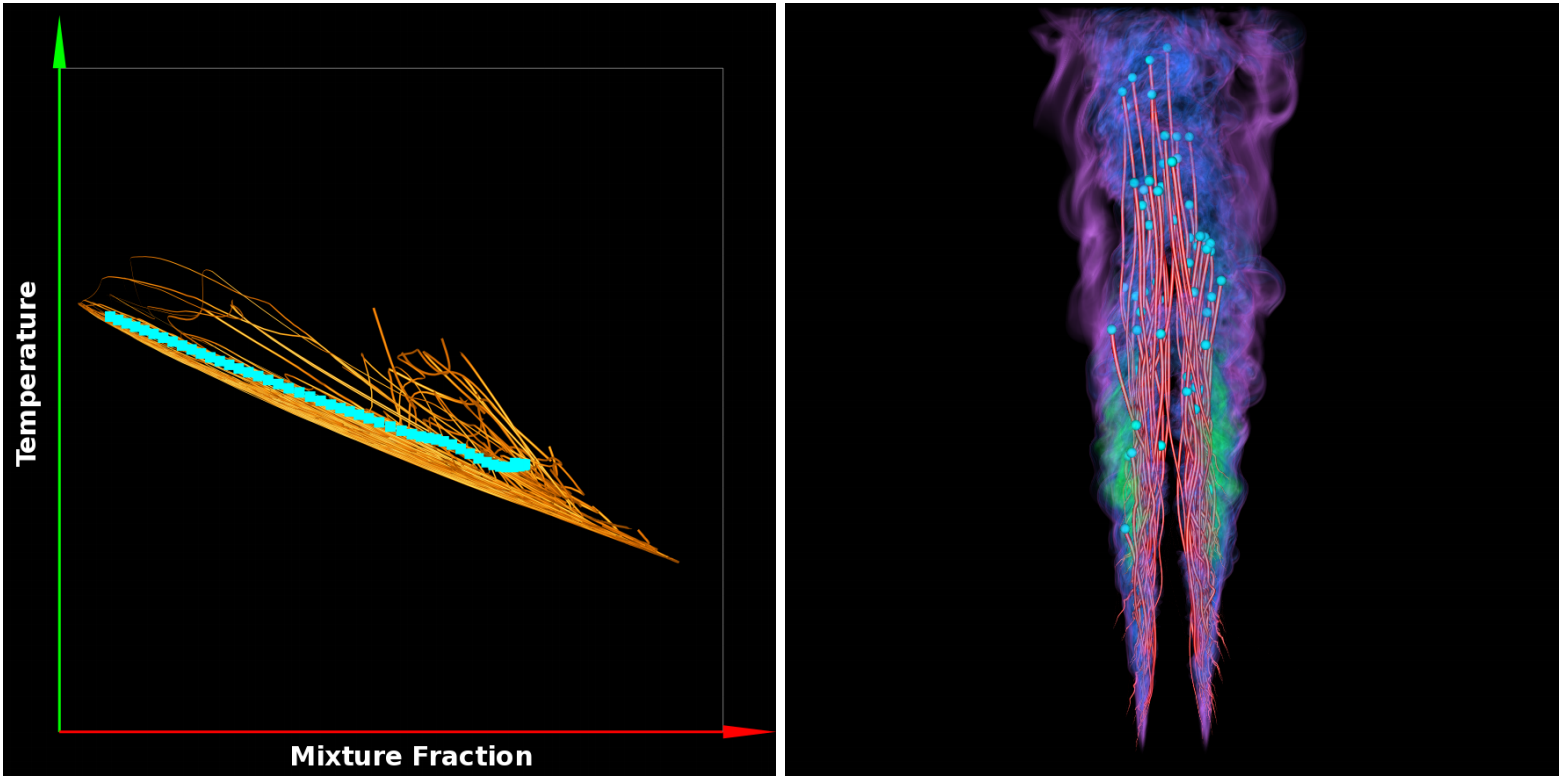
\includegraphics[width=\textwidth]{figures/wei_particle_clusters.png}
    \caption{Hybrid visualization of particle trajectories in phase space (left)
    and physical space (right) of an ethylene/air jet flame. Image source:
    Wei \etal~\cite{Wei2011}.}
    \label{fig:wei_particle_clusters}
\end{figure}
%
% subsubsection special_methods_for_turbulent_combustion (end)
%
% subsection post_processing (end)
%
\subsection{In-Situ Processing} % (fold)
\label{sub:in_situ_processing}
%
With disk space and I/O speed being the bottleneck in today's large-scale
simulations, in-situ approaches to visualization and analysis have gained
popularity through the last 15 years.
%
Here, the visualization and analysis of the data is performed in parallel or
interleaved with the simulation, without first writing it to a hard disk.
%
This allows for the analysis of the complete simulation output, rather than
the infrequent snapshots that are used in post-processing approaches.
%
Ma gave an overview of the problems and opportunities inherent in in-situ
visualization~\cite{Ma2009}.
%

%
A central complication of in-situ approaches is the loss of flexibility and
interactivity.
%
Large simulations typically need to be submitted to a job queue before they are
started on a supercomputing cluster.
%
This means that there might be a significant waiting time before any results can
be viewed.
%
It is often unreasonable to expect that an analyst is present to look at the
data while some interesting feature or behavior can be observed during the
simulation.
%
Additionally, simulations can take several days or even weeks to complete.
%
This makes an exploratory analysis of the data very challenging.
%
Many in-situ approaches therefore have a batch processing character, where
visualization and analysis tasks are defined beforehand and are then
carried out during the simulation with little to no user input.
%
The user then explores the significantly smaller results, which ideally still
contain all relevant information.
%

%
Another problem is performance.
%
Since large simulations can already take a very long time, researchers are
reluctant to accept a significant increase in computing time in return for
visualization.
%
The simulation data is distributed across the nodes of the supercomputer to
optimize the simulation time.
%
This is not necessarily an optimal distribution for visualization tasks.
%
The result can be a significant communication overhead, which is a major
bottleneck in supercomputing clusters.
%
In-situ algorithms need to be carefully crafted to find a good balance between
communication overhead and efficiency gained by data reorganization.
%

%
A lot of groundwork is being done to create the foundations for successful
in-situ processing.
%
We will first give an overview of these technical contributions and then present
some examples for specific in-situ visualization and analysis methods.
%
\subsubsection{Technical Foundations} % (fold)
\label{ssub:technical_foundations}
%
In-situ processing is a complex task not only from a conceptual, but also from a
software engineering perspective.
%
In-situ algorithms need to run on large supercomputers in parallel or even on
the same nodes as the simulations.
%
They need to somehow get the relevant data from the simulation and they need to
be efficient enough to not slow it down by an unreasonable amount.
%
Communication between computing nodes runs over relatively slow network
connections, requiring different parallel algorithms than for shared-memory
multi-core architectures.
%
Additionally, computing nodes often do not have dedicated graphics hardware,
which makes software rendering a necessity.
%
All this requires a solid technical foundation of systems and algorithms that
facilitate the visualization and analysis tasks that eventually derive insight
from simulations.
%

%
The two most popular open source software packages for scientific visualization,
ParaView and VisIt, both include an extension for in-situ visualization.
%
In the case of ParaView, it is called Catalyst~\cite{Ayachit2015}.
%
VisIt's in-situ library is LibSim~\cite{Whitlock2011}.
%
Both require a certain amount of instrumentation of the simulation code to
function.
%
If a simulation code has been interfaced with the visualization software, it
communicates its data to parallel visualization server processes that are
launched together with the simulation and eventually to a client that
allows a similar interaction as if the data was loaded from a file.
%
In addition, the user can define non-interactive batch visualization tasks that
are executed regularly and produce images or data files.
%

%
Larsen \etal presented a simpler and more flexible system that only supports
batch visualization with Strawman~\cite{Larsen2015}.
%
It is based on EAVL~\cite{Meredith2012}, a visualization library that is
designed fundamentally to run on massively parallel architectures.
%
Libraries with similar goals exist in DAX~\cite{Moreland2011} and
PISTON~\cite{Lo2012}.
%
All three have merged their efforts into a single project:
VTK-m~\cite{Moreland2016}.
%
The goal is to develop a native visualization library for supercomputers and
other highly parallel architectures that can be a basis for scientific
visualization in a future with steadily growing data sizes and a growing need
for in-situ capabilities.
%

%
Many existing tools for in-situ processing require changes to the simulation
code in order to receive data from it.
%
This can be an additional obstacle for the adaption of these tools by simulation
scientists.
%
One possibility to reduce this invasiveness is to link the visualization and
analysis tasks to the I/O library the simulation code uses to write out its
data~\cite{Vishwanath2011,Biddiscombe2011,Dorier2013}.
%
This unifies the tasks of writing snapshots to disk, analyzing and visualizing
them into the same framework and effectively decouples them from the simulation
itself.
%
The Freeprocessing system~\cite{Fogal2014} takes an even less invasive approach.
%
It places itself between the I/O calls and the simulation code at library load
time, requiring no changes to the simulation code at all.
%

%
Another focus of research has been dedicated to improving performance.
%
Researchers have tried sophisticated load-balancing algorithms to take advantage
of unused resources during a simulation run for visualization and analysis tasks
\cite{Zheng2013}.
%
A popular alternative to processing the data on the same computing nodes as the
simulation is to offload the data onto a separately allocated number of staging
or processing
nodes \cite{Zheng2010,Abbasi2010,Abbasi2011,Docan2011,Docan2012,Bennett2012}.
%
Using this approach, which is often called \emph{in-transit} processing, the
simulation is only slowed down by the time it takes to copy the data to the
staging nodes, where processing can happen in parallel to the next simulation
step.
%
Some work has also been done to optimize existing parallel rendering algorithms
for use on supercomputing
clusters \cite{Yu2008,Kendall2010,Moreland2011a,Cavin2012,Nonaka2014,Grosset2016}.
%

%
In all of the works presented above, efficiency and convenience of in-situ
processing was the focus.
%
The second major problem, namely the lack on interactivity, has been addressed
to a lesser extent.
%
Maybe that is because it is much harder to solve.
%
The challenge is to enable an exploratory analysis of the simulation data, \ie,
with little to no prior knowledge of what one is looking for.
%
This stands in direct conflict with the goal of in-situ approaches to reduce the
amount of data that has to be stored to disk.
%
In order to reduce the data, one must know what is or is not important.
%
A small number of works has tried to address this issue.
%

%
One obvious possibility is to compress the data using some generic concept of
``importance'' that is not dependent on a particular application.
%
Lakshminarasimhan \etal~\cite{Lakshminarasimhan2011} developed such an algorithm
whose core idea is to sort the data before compression to take advantage of the
special characteristics of scientific data.
%
With a compression ratio of about 1:7, this approach allows to store a much larger
amount of data while still retaining complete freedom for an exploratory
analysis of the data.
%

%
Another approach has been proposed by Kageyama and Yamada~\cite{Kageyama2014}
and Ahrens \etal~\cite{Ahrens2014}:
%
Produce a database of visualizations that the user can explore later.
%
During the simulation, rendered images are produced for a range of parameters
of the same visualization.
%
For example, isosurfaces of different variables with different iso-levels are
rendered from different camera angles and stored into the database.
%
The user can then select a set of parameters after the fact, retrieve the
best fitting image from the database, and even compose multiple images into
a combined visualization.
%

%
All these contributions address different issues that need to be solved for
in-situ processing to become successful.
%
Since the field is still in its infancy, no clear favorites have emerged yet and
a definitive in-situ framework has yet to be developed.
%
% subsubsection technical_foundations (end)
%
\subsubsection{Special Visualization and Analysis Methods} % (fold)
\label{ssub:visualization_and_analysis_methods}
%
Although most work in the field of in-situ visualization has been done to lay
the groundwork for efficient basic visualization, there have been some
developments of more specialized in-situ methods.
%
We will discuss some examples here that are applicable to the field of turbulent
combustion.
%

%
The first in-situ visualization methods focused on rendering images for
monitoring the simulation.
%
Yu \etal~\cite{Yu2010} used their parallel direct volume rendering and image
compositing algorithm \cite{Yu2008} to display scalar variables in combustion
simulations together with particles advected with the flow.
%
This gives an idea about the evolution of the simulation but does not allow for
quantitative analysis of the data.
%
Tikhonova \etal~\cite{Tikhonova2011} developed a more flexible approach by
rendering the data into an intermediate representation that stores an
attenuation function instead of color values.
%
The transfer function can then be changed after the fact, allowing for a certain
degree of interactivity (see \cref{fig:tikhonova_tf}).
%
This approach fits well with the image databases discussed in the previous
section \cite{Kageyama2014,Ahrens2014}.
%
\begin{figure}[t]
    \begin{captionbeside}{
        Retroactive adjustment of the transfer function in direct volume
        renderings of a turbulent jet flame. Left: original transfer function.
        Middle: Opacity modulation. Right: Opacity modulation and
        re-colorization. Image source: Tikhonova \etal~\cite{Tikhonova2011}.
        \label{fig:tikhonova_tf}
    }[o]
        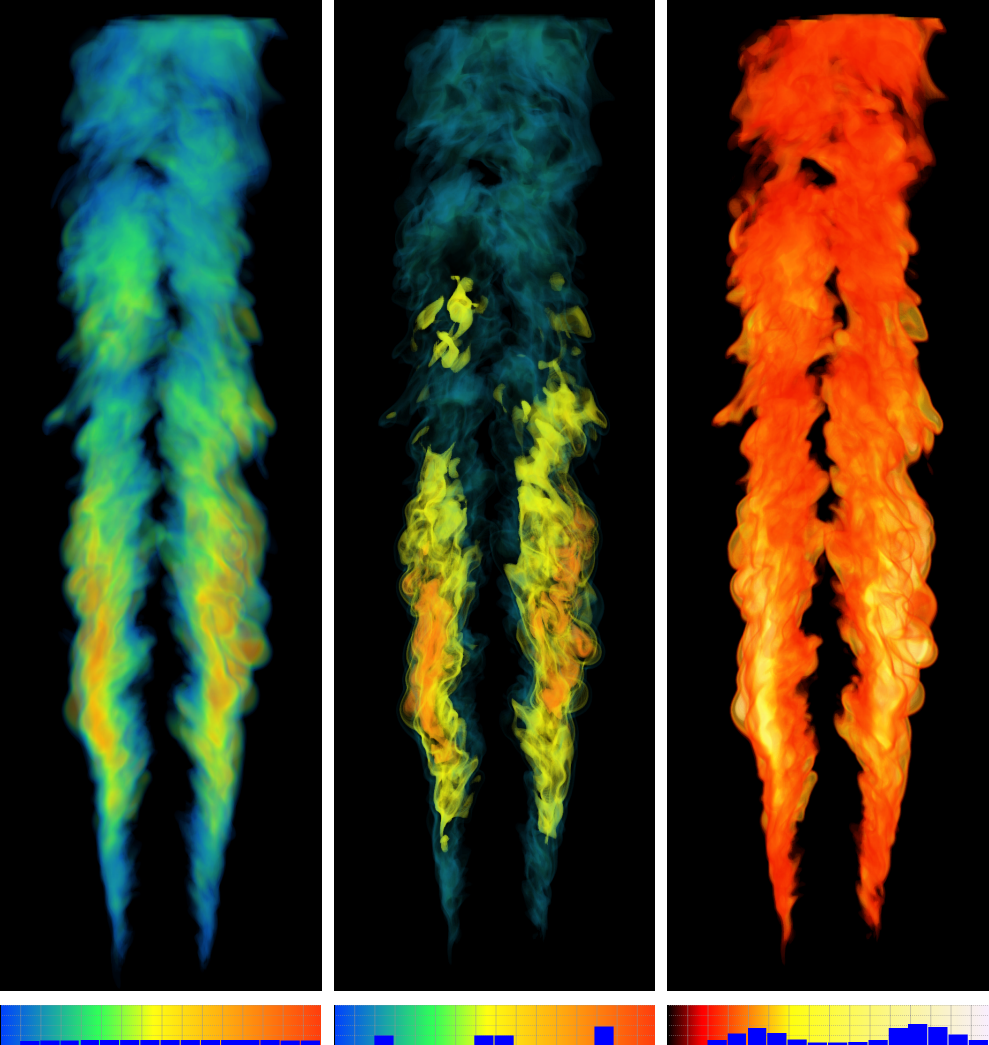
\includegraphics[width=0.6\textwidth]{figures/tikhonova_transfer_function.png}
    \end{captionbeside}
\end{figure}
%

%
Moving to more analytic approaches, several works have addressed the extraction
and tracking of volumetric features.
%
Chen \etal~\cite{Chen2003} presented an in-situ system for tracking volumetric
features defined by thresholding.
%
Zhang \etal~\cite{Zhang2012} used the \ac{DOC} algorithm \cite{Quiroz2008} to
identify and track features defined by clusters in state space during a
simulation run.
%
This can for example be used to identify and track burning regions in combustion
simulations.
%
The IFDT framework \cite{Duque2012} takes a more flexible approach by letting a
user interactively pick individual structures to track.
%
The system includes a machine learning component that learns to identify the
features picked by the user based on their visual properties.
%
This is intended to be more robust than detection based on thresholds which
might not be applicable over long time periods.
%
Ye \etal~\cite{Ye2015} combined image-based visualization with feature tracking
by storing rendered depth maps of multiple isosurfaces.
%
These are later used to create visualizations and to track features in image
space based on their depth information.
%
\Cref{cha:flame_surface_tracking} of this thesis presents an in-situ tracking
algorithm for surfaces which explicitly captures temporal correspondence and
tangential movement of surface points.
%

%
The idea of precomputing an intermediate representation of the data in-situ and
then exploring it post-hoc has also been applied in some more specialized
visualization systems.
%
Landge \etal~\cite{Landge2014} adapted the computation of segmented merge trees
\cite{Bremer2009,Bremer2011} for in-situ applications.
%
This allows for an interactive exploration of the space of possible thresholds
or iso-levels for scalar variables.
%
Ye \etal~\cite{Ye2016} proposed a system for exploring joint field/particle
datasets as are for example produced by some combustion \ac{DNS} codes.
%
They compute \acp{PDF} to represent the field data and reorganize the particle
data into a more efficient scheme.
%
Researchers can then explore the \acp{PDF} in a post-hoc tool and define queries
to select matching particle data.
%
A space-saving representation for post-hoc analysis of premixed combustion data
is presented in \cref{cha:sparse_representation} of this thesis, although not as
an in-situ algorithm.
%
%
% subsubsection visualization_and_analysis_methods (end)
%
% subsection in_situ_approaches (end)
%
% section visualization_for_turbulent_combustion_simulations (end)
%
% chapter turbulent_combustion (end)

%
% part background (end)
%
\part[Analysis and Visualization of the Flame Surface
         in Turbulent Combustion Simulations]
        {Analysis and Visualization\\of the Flame Surface\\
         in Turbulent Combustion Simulations} % (fold)
\label{part:flame_vis}
%
\chapter[Sparse Representation for Turbulent Premixed Flames]
        {Sparse Representation and Visualization for Turbulent Premixed Flames} % (fold)
\label{cha:sparse_representation}
%
\tikzset{external/export=false}
\begin{tikzpicture}[overlay]
    \node[paperheader]
        at ([yshift=1.2cm]mychapanchor-\arabic{chapter} -| current page text area.west)
        (banner_fst) {%
            \parbox[b]{0.5\textwidth}{%
            This chapter is based on the publication:\\
            \fullcite{Oster2014}}%
    };
\end{tikzpicture}
\tikzset{external/export=true}
%
\vspace{-2\baselineskip}\lettrine[loversize=0.02, lhang=0.03,
findent=-0.7pt]{T}{he development} and validation of flamelet models is one of
the central applications of \ac{DNS}.
%
As already mentioned in \cref{sub:the_flamelet_assumption}, the flamelet
assumption is one of the most important simplifications applied for modeling
turbulent combustion.
%
It states that a turbulent flame behaves like a collection of strained laminar
flames (``flamelets'') located side-by-side on the flame surface.
%
This assumption is most often applicable to premixed flames and essentially
allows to treat the flame as a \ac{2D} manifold.
%

%
The analysis of \ac{DNS} data in the context of flamelet modeling can have
two purposes: validation of existing flamelet models, or development of new
models.
%
In both cases, it is necessary to extract flamelet data from the \ac{DNS}.
%
This is often done by sampling the simulation variables along lines orthogonal
to the flame surface (see \eg, \cite{Zistl2009}).
%
The single flamelets obtained from this are then used for statistical analysis,
for example to check model assumptions or discover correlations that can be
incorporated into new models.
%

%
In this chapter we propose a sparse representation for premixed flames that
explicitly encodes flamelets and readily supports flamelet-related analysis
tasks.
%
This representation is significantly smaller than storing the full DNS data,
which enables the analysis of a larger number of time steps per simulation run.
%
We also propose a novel visualization based on this data that augments
traditional statistical analysis with a visual component.
%
If necessary, full scalar fields on the original grid can be reconstructed
from the sparse representation to retain full flexibility for post-processing.
%

%
In spirit, the approach we present is similar to existing works that propose
computing a smaller representation of the data that can later be used for
analysis.
%
Lakshminarasimhan \etal{} presented the ISABELA compression algorithm
\cite{Lakshminarasimhan2011} and a tool for querying the compressed data
\cite{Lakshminarasimhan2011a}.
%
Bremer and Landge~\cite{Bremer2009,Bremer2011,Bremer2010,Landge2014} presented
multiple works based on the computation of segmented merge trees that facilitate
a post-hoc exploration of thresholds on scalar fields.
%
Ye \etal{}~\cite{Ye2016} condensed high-resolution grid data into block-wise
probability density functions that can later be explored efficiently.
%

%
The rest of this chapter is organized as follows:
%
We first introduce our approach for constructing a sparse representation of the
flame in \cref{sec:compression}.
%
We then introduce our novel visualization techniques based on this
representation in \cref{sec:visualization}.
%
\Cref{sec:reconstruction} describes the reconstruction of full scalar fields and
evaluates the compression ratio and reconstruction quality we achieve.
%
Finally, we provide a discussion and conclusion in \cref{sec:conclusion}.
%
%
\section{A Sparse Representation for Premixed Flames}
\label{sec:compression}
%
As mentioned before, a flamelet lives on \ac{1D} lines orthogonal to the flame
surface.
%
If we extract the flame surface and store all flamelets as \ac{1D} profiles of
the simulation variables orthogonal to this surface, we have a full
representation of the flame front.
%
Since the variation of the simulation variables is typically small tangential to
the surface, we can store a sparse selection of flamelets and still represent
the flame with adequate accuracy.
%
This is the idea behind our sparse representation for premixed flames.
%

%
The transformation of raw \ac{DNS} data into our sparse representation consists
of three steps:
%
\begin{enumerate}
	\item Seed points on the flame surface.
	\item Sample the simulation variables along lines orthogonal to the flame
	surface, emanating from the seed points.
	\item Approximate the resulting profiles by models, reducing each profile to
	a set of model parameters.
\end{enumerate}
%

%
We extract the flame surface as an isosurface and distribute seed points on it
using random sampling adaptive to the surface curvature.
%
\ac{1D} profiles are then extracted orthogonal to the flame surface.
%
The profiles are centered on the surface points and have a limited length to
include the maximum flame thickness.
%
In this way, only the data of the flame front is captured, and the large, almost
constant areas containing fresh gases and hot products are discarded.
%
We only store the profiles of variables related to chemistry, namely the
temperature, heat release and species mass fractions.
%
We ignore the velocity and pressure fields, as they do not exhibit the same
structure as the chemical variables and can not be accurately represented by
\ac{1D} profiles in the flame front only.
%

%
Variables are grouped into three classes: \emph{Reactants} have high
values outside of the burnt region and low values inside,
\emph{products} are the opposite, and \emph{intermediates} occur near the flame
surface between unburnt and burnt regions but have low values on either side.
%
This behavior can be modeled with few degrees of freedom, reducing the amount of
data even further.
%
The information that has to be stored in the sparse representation consists of
the locations and directions of the profile lines, the model parameters for each
variable and profile line, and the full flame surface mesh for visualization.
%
% The compression $C$ then becomes a transformation from a set
% of simulation variables $(V_1, \dotsc, V_v)$ to a tuple consisting of the
% locations and directions of the profile lines, $(\vp_i, \vr_i)$, and
% the model parameters for each variable and line, $\Phi$:
% \begin{equation}
% 	\begin{aligned}
% 		C(V_1, \dotsc, V_v) &= ((\vp_i, ~\vr_i), ~\Phi^{V_1}, \dotsc, \Phi^{V_v}), ~ i = 1, \dotsc, n\\
% 		\text{with } \Phi^V &= \phi^V_{ij}, ~ j = 1, \dotsc, m \text{ .}\\
% 	\end{aligned}
% \end{equation}
% Here, the set of model parameters for all lines of variable $V$ is denoted as
% $\Phi^V \in \R^{n \times m}$, which is a matrix with entries $\phi^V_{ij}$,
% denoting the $j$-th model parameter of the $i$-th profile line.
%
We now describe how the lines are seeded, how the profiles are extracted from
those lines, and how these profiles are then approximated by simple models.
% 
\subsection{Strategy for Seeding Profile Lines} % (fold)
\label{sub:seeding}
%
\begin{figure}[t]
	\setlength\figurewidth\textwidth
	\centering
	\input{figures/flamecrossing_tikz}
	% \vspace*{-6mm}
	\tikzset{external/export=false}
	\caption{
		Cross section scheme of the flame surface with seeded points $\vp$.
		Profiles are sampled from profile lines $\vp(t)$ (arrows) at different
		locations on the flame surface. The minimum
		(\protect\tikz\protect\draw[thick, fill=mycolor3] circle
		[radius=0.8mm];), inflection (\protect\tikz\protect\draw[thick,
		fill=mycolor1] circle [radius=0.8mm];) , and maximum
		(\protect\tikz\protect\draw[thick, fill=mycolor4] circle
		[radius=0.8mm];) of the sigmoid shape are indicated on the profiles. }
	\label{fig:flamecrossing}
	\tikzset{external/export=true}
\end{figure}
%
Commonly, the flame surface in premixed combustion is defined as the
\num{0.5}-isosurface of a \emph{combustion progress
variable}~\cite{Poinsot2012}.
%
This variable is defined as $({T-T_u})/({T_b-T_u})$, where $T_u$ and $T_b$ are
the temperature of the burnt and unburnt gases, and varies between 0 and 1.
%
The choice of the iso-value is very robust for premixed combustion in the
flamelet regime.
%
Our experiments show that variations of $\pm \num{0.1}$ lead to isosurfaces with
Hausdorff distances less than \SI{2}{\percent} of the domain size.
%

%
Anchor points $\vp_i$ for profile extraction are distributed on this surface,
which we extract using \ac{CGAL}~\cite{Boissonnat2005}.
%
This yields a mesh with approximately uniformly-spaced vertices and edges of
approximately the same length as the voxel size in the original data.
%
%We first place a point into every surface voxel. 
%
% Sub-voxel sampling would not yield more information due to the smoothness of \ac{DNS}
% data. 
%
Since this results in a large number of vertices, we select only some of them as
seed points, using a rejection sampling based on local surface curvature.
%
%This results in a large number of seed points. We therefore reduce the number
%of points by a random process based on the local surface curvature. 
%
%We use a method described by Kindlmann et al.~\cite{Kindlmann2003} to 
%
We estimate the principal curvatures $\kappa_1$ and $\kappa_2$ at each vertex
(see, e.g., \cite{Kindlmann2003}).
%
The curvatures are then transformed into a seeding density by a logarithmic
function:
%
\begin{equation}
	\rho(\kappa_1, \kappa_2) =
		\frac{\ln(1 + \sqrt{\kappa_1^2+\kappa_2^2})}{q}\text{ .}
\end{equation}
%
Here, $q > 1$ steers the seeding density.
%
For each initial vertex, a uniformly distributed random number $r \in [0, 1]$ is
now generated, and the point is selected if $\rho < r$.
%
This results in few seed points in areas without curvature, and all vertices
being selected in areas where $\rho > 1$.
%
Areas of higher curvature get more seeds than less curved ones (see blue circles
in \cref{fig:flamecrossing}).
%
Hence, the storage size of the sparse representation depends on the surface
shape more than on the resolution of the data.
%
Adjusting $q$ changes the total number of seed points and balances size vs.
quality.
%
% The logarithmic shape of
% $\rho$ ensures that medium curvatures, which are most frequent, are not
% discarded as often, and sampling density is more even across areas of higher
% curvature. By allowing the density of the maximum curvature to drop below 1, it
% becomes possible to avoid overly dense seeding in high-curvature areas.
%
%\begin{figure}[t]
%	\begin{center}
%		\includegraphics[width=\linewidth]{figures/lineseeding.pdf}
%	\end{center}
%	\caption{
%	2D example of flame surface with seeded points. More points are seeded at
%	locations of high curvature.
%	}
%	\label{fig:seeded_points}
%\end{figure}
%
%
% subsection seeding (end)
%
\subsection{Extracting Profile Lines} % (fold)
\label{sub:profile_extraction}
%
Once the points $\vp_i$ are seeded, profiles of all variables are sampled at
regular intervals along lines $\vp_i(t)=\vp_i + t \cdot \vn_i$, with $\Norm{\vn_i}
= 1$ (\cref{fig:flamecrossing}).
%
% According to Shannon's theorem the step size is $\sfrac{1}{2}$ of the voxel
% size.
% 
Due to the high resolution and accuracy of \ac{DNS} data, trilinear
interpolation is sufficient.
%
The length of the line is chosen sufficiently large to cover the whole flame
front.
%
The resulting profiles are approximated by simple models to further reduce the
required storage space.
%
% The resulting profiles are discretely sampled functions
%
% \begin{equation}
% 	P_{ij}^V = V(\vp_i(t_j)), ~ i=1, \dotsc, n, ~ j = 1, \dotsc, m,~
% 	t_j = -\frac{\tau}{2} + \frac{j-1}{m-1} \cdot \tau \text{ ,}
% \end{equation}
%
% where $V$ is the variable from which the profiles are extracted, $n$ is the
% number of lines, $m$ is the number of sample points along the line, and $\tau$
% is the length of the line. We are assuming a uniform grid with voxels of $1$
% unit edge length for simplicity.
%
% subsection profile_extraction (end)
\subsection{Model-Based Data Approximation} % (fold)
\label{sub:fitting}
%
% address a review comment
%----
% Even though \ac{DNS} data are simulated without any model assumptions,
% it is reasonable to describe the data outcome of them via models for
% two reasons: i) the model-based description of the data does not negatively effect
% the simulation benefits of \ac{DNS} data being that \ac{DNS} data have a low
% simulation error because the simulation still runs with the raw data per time step;
% and ii) the models facilitates the treatment and extraction of such
% characteristic features which the domain experts want to investigate for
% data analysis purposes. In the following, the compression scheme steps are described in detail.
%----
Although the main advantage of \ac{DNS} is its high precision due to the lack of
modeling assumptions, we use models to describe its outcome in a lower-
dimensional form.
%
These models are sufficient to facilitate the analysis of the scalar fields we
intend.
%
Additionally, they reduce the space needed to store the sparse representation.
%

%
Reactants, intermediates, and products each have very similar profiles that can
be locally approximated by simple models.
%
Reactants and products tend to exhibit profiles with a sigmoid shape,
transitioning from a constant high/low value in the unburnt region to a constant
low/high value in the burnt region, passing an inflection point in between.
%
This behavior can be expressed by a model based on a sigmoid function.
%
Intermediate species have a maximum near the flame surface, decreasing on both
sides.
%
They are approximated by a model based on a Gaussian bell curve.
%

%
Small fluctuations that deviate from these models may occur but are not relevant
for the general shape.
%
Greater deviations appear if a sample line crosses the flame surface multiple
times, which happens if multiple parts of the flame front come close to each
other.
%
In such cases, the characteristic behavior occurs multiple times across the
profile.
%
To handle this, the instance closest to the anchor point is identified and
isolated from the others.
%
\subsubsection{Model for Reactants and Products} % (fold)
\label{ssub:model_for_reactants_products}
%
Sigmoid shapes are commonly expressed using the logistic function $1/(1+e^{-t})$,
which we extend with parameters $\gamma$, adjusting the slope at the inflection
and $a$, determining the limits of the function at positive/negative infinity:
%
\begin{equation}
	\mathfrak{s}(t,a,\gamma)
		= \frac{2a}{ 1 + e^{ (-2\frac{\gamma t}{a}) } } - a \text{ .}
\end{equation}
%

%
While this function can roughly approximate the profiles of reactants and
products, it has too few degrees of freedom to reproduce the different
curvatures of the profiles at both sides of the inflection point.
%
For this reason, we use two pieces of this function, joining smoothly at the
inflection point (\cref{fig:models}, top).
%
\begin{equation}
%	\begin{aligned}
		\mathfrak{S}(t, a_l, a_r, \gamma, x_m, y_m) =
		\begin{cases}
			\mathfrak{s}(t, a_l, \gamma) + y_m, &\text{if }  t \leq x_m\\
			\mathfrak{s}(t, a_r, \gamma) + y_m, & \text{if }  t > x_m\\
		\end{cases}
%		&\text{with } \sgn(\gamma) = \sgn(a_r) = \sgn(a_l) \text{ ,}
%	\end{aligned}
\end{equation}
%
where $(x_m, y_m)$ is the location of the inflection point, $\gamma$ is the
slope at the inflection and $y_m-a_l$ and $y_m+a_r$ are the limits of the
function approaching negative and positive infinity.
%
% subsubsection model_for_reactants_products (end)
%
\subsubsection{Model for Intermediate Species} % (fold)
\label{ssub:model_for_intermediate_species}
%
The profiles of intermediates resemble Gaussian bell curves.
%
Since minimum and maximum of the profiles of intermediate species can vary, it
is necessary to extend the standard bell curve with additional parameters $y_m$,
the value at the maximum, and $y$, the limit at infinity.
%
\begin{equation}
	\mathfrak{g}(t, x_m, y_m, \sigma, y)
		= e^{-\frac{1}{2}(\frac{t-x_m}{\sigma})^2}\cdot(y_m-y)+y \text{ .}
\end{equation}
%

%
Since the profiles tend to have a steeper slope on the unburnt side and some of
them do not reach zero on the burnt side, a two-sided model is once again needed
to accurately capture this behavior.
%
We join the two bell curves smoothly at their maximum point, resulting in a
model with six parameters:
%
\begin{equation}
	\mathfrak{G}(t, x_m, y_m, \sigma_l, y_l, \sigma_r, y_r) =
	\begin{cases}
		\mathfrak{g}(t, x_m, y_m, \sigma_l, y_l), & \text{if }  t \leq x_m\\
		\mathfrak{g}(t, x_m, y_m, \sigma_r, y_r), & \text{if }  t > x_m\\
	\end{cases}
\end{equation}
%
where $(x_m, y_m)$ is the location of the maximum, $\sigma_l$ and $\sigma_r$
determine the slope of the left and right part of the function and $y_l$ and
$y_r$ are the limits of the function approaching negative and positive infinity
(\cref{fig:models}, bottom).
%
% \begin{figure}[ht]
% 	\centering
% 	\setlength\figureheight{3cm} 
% 	\setlength\figurewidth{7cm}
% 	\input{figures/gaussmodel.tikz}
% 	\caption{Gaussian model}
% 	\label{fig:gaussmodel}
% \end{figure}
%
% subsubsection model_for_intermediate_species (end)
%
\subsubsection{Fitting the Models to the Profiles} % (fold)
\label{ssub:fitting_the_models}
%
We now approximate the profiles by fitting the models.
%
For the sigmoid model, we need the position, value and first derivative at the
inflection point as well as the minimum and maximum values of the profile on
both sides of the flame front.
%
For the Gaussian model, the location and value of the maximum near the flame
front have to be known, as well as the minimum values $y_l$ and $y_r$.
%
To robustly determine these feature points, we have to account for the two types
of deviations that may occur in the profiles as described above:
%
small fluctuations, and the profile entering and leaving the reaction zone
multiple times.
%

%
To eliminate small fluctuations, we filter the profiles with a Gaussian kernel
\cite{Jaehne2005}.
%
The kernel size depends on the size of the fluctuations but can be chosen quite
small.
%
For the test data (see \cref{sec:reconstruction}) we used a size of \num{6}
voxels, which translates to $\sigma = 1$.
%

%
Extrema are found at zero-crossings of the first derivative of the filtered
profile.
%
Possible shifts of the extrema due to the filtering are corrected by mapping
each maximum to the largest maximum, and each minimum to the smallest minimum in
the radius of the filter size, taking care that extrema do not switch sides.
%
For finding inflection points, we use the same approach but on the second
derivative.
%


%
Due to the possibility of crossing the flame surface multiple times (see $\vp_3$
in \cref{fig:flamecrossing}), we can find more feature points on the profile
than we need for our models.
%
We have to identify the ones closest to the anchor point.
%
For the sigmoid model, this is the inflection nearest to the center of the
profile.
%
The position and value of this point determine $x_m$ and $y_m$ of the sigmoid
model, while $\gamma$ is determined by the first derivative at the inflection.
%
The values of the first minimum and maximum left and right of the inflection
(depending on the sign of $\gamma$) determine $a_l$ and $a_r$.
%
The positions of these extrema, $x_l$ and $x_r$, are the boundaries of the
portion of the profile that the model is fitted to.
%
The rest of the profile, possibly containing other crossings of the flame
surface, is not considered, as those other crossings are already captured by
other profile lines seeded there.
%
\begin{figure}[t!]
	\centering
	\setlength\figurewidth{0.95\linewidth}
	\setlength\figureheight{2.2cm}
	\input{figures/models.tikz}
	\vspace*{-2mm}
	\caption{
	Sigmoid model (top) and Gaussian model (bottom) with examples of models
	fitted to a profile.}
	\label{fig:models}
\end{figure}
%
% \begin{figure}[t]
% 	\begin{center}
% 		\setlength\figureheight{2cm}
% 		\setlength\figurewidth{0.85\linewidth}	
% 		\input{figures/fit_sigmoid_5.tikz}\\
% 		\input{figures/fit_gauss_3.tikz}
% 	\end{center}
% 	\caption{
% 	Top: Fitting the sigmoid model to a profile of temperature.
% 	Bottom: Fitting the Gaussian model to a profile of \ce{H2O2}.
% 	The non-constant data values outside the fitted range show that the profile
% 	crosses the reaction zone multiple times.
% 	}
% 	\label{fig:fitting_models}
% \end{figure}
%

%
For the Gaussian model, the maximum nearest to the center determines $x_m$ and
$y_m$, while the values of the closest minima to both sides determine $x_l$ and
$x_r$, as well as $y_l$ and $y_r$.
%
Further extrema are ignored.
%
For both models, if there are no extrema on either side of $x_m$, the values at
the ends of the profiles are chosen instead.
%

% \begin{figure}[ht]
% 	\begin{center}
% 		\setlength\figureheight{2cm}
% 		\setlength\figurewidth{0.85\linewidth}
% 		\input{figures/fit_gauss_3.tikz}
% 	\end{center}
% 	\caption{
% 	Fitting the Gaussian model to a profile of \ce{H2O2}. The values outside of
% 	the fitted range show that the profile crosses the reaction zone three times.
% 	}
% 	\label{fig:fitting_gaussian}
% \end{figure}

%
While the feature points on the profile already determine all parameters for the
sigmoid model, the values for $\sigma_l$ and $\sigma_r$ of the Gaussian model
still have to be found.
%
We obtain an initial guess for $\sigma_{l/r}$ by transforming the intervals of
the profile between $x_l$ and $x_m$ and between $x_m$ and $x_r$ into the
interval $[0, 1]$ and regarding them as halves of two symmetric \acp{PDF}.
%
The variance of a discrete random variable $X$ with the \ac{PDF} $p(x)$ and
expected value $\mu$ is given by: $\var(X) = \int p(x) \cdot (x-\mu)^2 ~dx$.
%
Since for a normal distribution, the variance is $\sigma^2$, we can directly use
this equation on our transformed profiles.
%
We then refine this estimate with a simple optimization scheme such as Newton's
method to find the optimal fit.
%

% As an initial guess, we use the fact that for a normal
% distribution, $\sigma^2$ is equal to the variance. Since our model, like the
% normal distribution, is based on the Gaussian function, we can employ a method
% similar to estimating the variance of a probability density function (pdf) for
% determining an initial guess for $\sigma_l$ or $\sigma_r$. 
% By transforming each side of our Gaussian model into the value range $[0, 1]$
% and regarding it as one half of a symmetric pdf, we can directly employ the
% above equation to obtain an estimate for both parameters. We then refine this
% estimate with a simple optimization scheme such as Newton's method to find the
% optimal fit.

% Our profiles are not probability mass functions but by transforming them into
% something similar, we can use the same method to estimate a pseudo-variance and
% hence a good guess for $\sigma_{l/r}$. The values between $x_m$, which is our
% pseudo-$\mu$, and the nearest minimum to one side give us the basis for one half
% of a pseudo-pmf. By subtracting the minimum value and dividing the resulting
% values by twice their sum, we get something resembling one half of a pmf, which
% we can insert into equation \eqref{eqn:variance}, assuming it is symmetric
% in $x_m$. The resulting equation for estimating $\sigma_l$ is:
% \begin{equation}
% 	\begin{aligned}
% 	\sigma_li^2 =  &2 \cdot \sum_{j | x_li \leq x_ji \leq x_mi} \tilde{P}_ij^V \cdot (x_ji-x_mi)^2\\
% 	\tilde{P}_ij^V = &\frac{P_ij^V-y_li}{2 \cdot \sum_{j | x_li \leq x_ji \leq x_mi} P_ij^V-y_li}
% 	\end{aligned}
% \end{equation}
% Where $\tilde{P}_ij^V$ is the profile $P^V_ij$ between $x_li$ and $x_mi$,
% transformed into a half pmf like described. An estimate of $\sigma_ri$ can be
% determined in the same way.

% If the profile were perfectly similar to a normal distribution, this estimate of
% $\sigma$ would mean a perfect fit of the model to the data. If this is not the
% case, even small deviations can lead to an estimate that is not optimal. Finding
% the optimum in least squares sense is a nonlinear problem. Due to the good
% estimate we have, we can employ a simple optimization scheme such as Newton's
% method to find the solution with very few steps.

% For each profile
% line, we first determine the inflection point nearest to the center of the
% profile. We then find the nearest maximum or minimum at both sides of the
% inflection. The position, value and slope of the inflection as well as the
% positions and values of the extrema at both sides provide all necessary
% parameters of the model. 

% The parameter matrix $\Phi^V_{\textnormal{rp}}$ of the sigmoid model for reactants
% and products is
% \begin{equation}
% \Phi^V_{\textnormal{rp}} =
% 	(a_{li}, a_{ri}, m_i, x_{mi}, y_{mi}, x_{li}, x_{ri}),~
% 	i=1,\dotsc,n \text{ .}
% \end{equation}
%For intermediate species, the Gaussian model $G$ is fitted to the data. 
% Here,
% the maximum of the profile that is nearest to the anchor point at the center is
% first located. The minima at both sides of this maximum then give the boundaries
% of the relevant crossing of the flame surface, and the values for the limits
% $y_l$ and $y_r$ at both sides. To determine $\sigma_l$ and $\sigma_r$, we
% estimate an initial guess by regarding the profile between the left minimum and
% the central maximum, and the profile between the maximum and right minimum as
% halves of a transformed probability mass function. The optimal values are then
% found by minimizing the mean square error between data and model via Newton's
% method, starting at the initial guess estimated in the previous step. 
% The parameter matrix $\Phi^V_{\textnormal{int}}$ of the Gaussian model for
% intermediate species is 
% \begin{equation}
% \Phi^V_{\textnormal{int}} =
% 	(x_{mi}, y_{mi}, \sigma_{li}, y_{li}, \sigma_{ri}, y_{ri}, x_{li}, x_{ri}),~
% 	i=1,\dotsc,n \text{ .}
% \end{equation}

%
With this, the original data is now described by the flame surface mesh, the
$\vp_i$ and $\vn_i$ of the profile lines, and the model parameters for each
profile line and variable.
%
For the sigmoid model, this is $(a_{li},$ $a_{ri},$ $\gamma_i,$ $x_{mi},$ $y_{mi},$
$x_{li},$ $x_{ri})$ for each profile line.
%
For the Gaussian model, the parameters are $(x_{mi},$ $y_{mi},$
$\sigma_{li},$ $y_{li},$ $\sigma_{ri},$ $y_{ri},$ $x_{li},$ $x_{ri})$.
%
This comprises our sparse representation of the flame, with the flame surface
represented by the surface mesh and flamelets represented by the profile lines
orthogonal to the surface.
%
% subsubsection fitting_the_models (end)
%
% subsection fitting (end)
%
% section compression (end)

%
\section{Construction and Visualization of Feature Surfaces}
\label{sec:visualization}
%
The flamelets extracted as profiles in the previous step can directly be used
by combustion researchers for statistical analysis of the whole flame front.
%
We will not go into detail about this here, as it is outside the scope of this
work.
%
In this section, we present a novel visualization based on the feature points
extracted on the profiles that augments the statistical approach with a visual
analysis component.
%

%
The model parameters $x_l$, $x_m$ and $x_r$ (see \cref{fig:models}) describe
three classes of feature points on the profiles: \emph{minimum} (min),
\emph{maximum} (max) and \emph{inflection point} (infl).
%
% Using the position and direction of the profile lines, we transform those
% feature points into points in space. These points can describe a feature surface
% through the points of steepest slope, local maximum function values, etc.,
% depending on which feature point class is chosen, revealing more about the
% scalar fields than a simple isosurface can.
% 
These feature points span feature surfaces of the respective variables that can
have physical or chemical significance.
%
For example, the surfaces of maximum heat release or maximum concentration of a
radical are sometimes used as alternative definitions of the flame surface.
%
The feature surfaces of maximum and minimum temperature bound the flame front
and indicate the flame thickness.
%
Investigating the shapes and local distances of these surfaces gives insight
into the local combustion process and how it is affected by turbulent flow.
%
We now describe the construction of those feature surfaces and their
visualization.
%
% This section describes techniques to visualize feature surfaces -- i.e.,
% surfaces of interest -- of the DNS data. For this, by having the above
% introduced Sigmoid and Gaussian model as sparse DNS data representation,
% different classes of feature points w.r.t. the flame simulation can be revealed.
% These classes are \emph{maximum} $t_{max}$, \emph{inflection point} $t_t$, and
% \emph{minimum} $t_{min}$. They are related to the model's functions, which
% Figure~\ref{fig_models} illustrates. Based on that, we introduce the
% construction of feature points for all models of the DNS data.
%
% \begin{figure}[t!]
%     \centering
%  	\resizebox{240pt}!{\includegraphics{figures/models.pdf}}
% 	\caption{\label{fig_models}%
% 		Feature point classes: minimum $t_{\min}$, inflection point $t_{t}$,
% 		and maximum $t_{\max}$ of Sigmoid and Gaussian model.
% 	}
% \end{figure}
%
%
\subsection{Feature Point Construction}
%
The positions of the feature points on the profiles represent
intersections with the corresponding feature surfaces in the original data.
%
By shifting the anchor points $\vp_i$ onto the intersections with a specific
feature surface, we transform them to a feature point set sampling this surface
(see \cref{fig:featurepoints}, left).
%
Considering a profile line $\vp(t)$ anchored on the flame surface $S$, the
position of a feature point $\vp(t_f)$ with $f \in \{\text{min}, \text{max},
\text{infl}\}$ is given by
%
\begin{equation*}
	\vp(t_{f})=\vp + t_f \cdot \vn.
\end{equation*}
% with $t_{n}$ being the normalization
% \begin{equation}
% 	t_{n}= - \frac{ \vp \cdotp \vr }{ ||\vr||^2 }
% 		+ \sqrt{   
% 			(\vp\cdotp\vr)^2
% 			- \frac{ ||\vp||^2-\tau^2 }{ ||\vr||^2 }
% 		}. \nonumber
% \end{equation}
%
% It is based on the model distance $\tau$ and the model's feature point
% distance $t_f$, as illustrated in Figure~\ref{fig_pointcloud} (middle).
%
Here, $t_f$ is the shift value for the respective feature surface given by
$x_l$, $x_m$ or $x_r$ of the corresponding profile.
%
For example, the shift values $t_{\textnormal{max}}$ for the surface of maximum heat
release are obtained by the $x_m$ values of the heat release profiles.
%
Having constructed these feature points is the first step in constructing a
feature surface, which we detail in the following section.
%
% \begin{figure}[t]
%     \centering
%  	\resizebox{250pt}!{\includegraphics{figures/pointcloud.pdf}}
% 	\caption{\label{fig_pointcloud}%
% 	Revealing a feature point set based on flame surface and data models: (left)
% 	Initial flame surface $S$ and its profile lines $\vp_i(t),
% 	i=1,\dots,n$ given by point $\vp_i$ and its direction vector
% 	$\vr_i$. (middle) A potential configuration of parametrized Gaussian
% 	models for each profile line. Please note that the model's abscissa is
% 	aligned with the related direction vector. For illustration, the maximum
% 	$t_{max_i}$ is emphasized for each model. Of course, also further classes of
% 	feature points as well as the Sigmoid model could be considered. (right)
% 	With the aid of the profile line and model, the position of the feature
% 	point, e.g. the maximum, in space can be reveled by
% 	$\vp_i(t_{max_i})$. All those feature points define a point set of
% 	feature points. By considering a potential surface running through all
% 	feature points a feature surface, here a maximum surface $S_{t_{max}}$
% 	(light red), is found. }
% \end{figure}

%
\subsection{Feature Surface Construction}
%
Remember that during the transformation to the sparse representation, an
isosurface mesh $M$ representing the flame surface $S$ was extracted.
%
The profile lines were seeded at vertices of this mesh.
%
For each vertex $\vp_i$ on the flame surface mesh we therefore know the position
of a point on the feature surface $S_f$ by the corresponding shift value
$t_{fi}$ and the direction of the profile line $\vn_i$
(\cref{fig:featurepoints}, left).
%
% Revealing a feature surface is a non-trivial task due to reasons of ambiguity:
% obviously, an infinite number of surfaces can be fitted to the point set. Thus,
% the construction issue ends up in a selection issue, i.e., selecting one
% relevant surface. To solve this selection issue, we subsequently exploit the
% knowledge about the relation between the feature point set and the flame
% surface.
%
% \begin{figure}[t]
%     \centering
%  	\resizebox{245pt}!{\includegraphics{figures/featurecontourconstruction.pdf}}
% 	\caption{\label{fig_featurecontourconstruction}%
% 	Relations between flame surface $S$, flame mesh $M$, profile lines
% 	$\vp_i(t)$, and feature point set $\vp_i(t_f)$: (left) Initial
% 	flame surface $S$, its profile lines $\vp_i(t), i=1,\dots,n$ given by
% 	points $\vp_i$ and direction vectors $\vr_i$, and a mesh $M$
% 	of the flame surface, given by the points $\vm_j,j=1,\dots,k$ (light
% 	blue) and its edges (black lines) based on Marching Cubes algorithm. (right)
% 	In addition, the relations between a feature point set and the profile lines
% 	are illustrated: start points $\vp_i$ are not aligned/related to a
% 	vertex points $\vm_j$ of flame surface mesh $M$, i.e., start points
% 	and vertices have different positions. }
% \end{figure}
%
% To construct a feature surface from a feature point set, we use our knowledge
% about the relation between the feature point set and the flame surface.
% Note that the flame surface $S$ equates to an isosurface of the data. An iso-
% surface mesh $M$ of the flame surface was extracted during the transformation to
% the sparse representation. A feature surface $S_f$ does not equate to an iso-
% surface. Therefore a mesh $M_f$ representing the feature surface is not as
% easily extracted from the data. However, the position of a point on the feature
% surface is known for every point $\vp_i$ by the corresponding shift value
% $t_{f_i}$ and the direction of the profile $\vr_i$
% (Figure~\ref{fig:featurepoints} (left)).
%
% Therefore, a mesh $M$, discretely representing the flame surface $S$, can be
% revealed by using Marching Cubes \cite{Lorensen:1987:CG}. Furthermore, a feature
% surface $S_f$ does not equate to an isosurface. Thus, a mesh $M_{f}$,
% discretely representing the feature surface $S_f$, cannot be revealed using,
% e.g., Marching Cubes.
%
The idea is to transform the flame surface mesh $M$ into a feature surface mesh
$M_{f}$ representing the feature surface.
%
%This can be done by exploiting the relations between the feature points set and
%the flame surface mesh.
\begin{figure}[t!]
	\centering
	% \def\svgwidth{0.8\textwidth}
	% \import{figures/}{featurepoints.pdf_tex}
	\input{figures/featurepoints_tikz}
	\tikzset{external/export=false}
	\caption{Construction of feature points and feature mesh (simplified \ac{2D}
	representation).
	%
	Left: Construction of feature points (\protect\tikz\protect\draw[thick,
	fill=black] circle [radius=0.8mm];) by shifting anchor points
	(\protect\tikz\protect\draw[thick, fill=white] circle [radius=0.8mm];)
	along their normals.
	%
	% Left: Feature points are constructed by shifting the anchor points $\vp_i$
	% on the flame surface $S$ along their normal vectors $\vn_i$ by amount
	% $t_f$ taken from the model parameters (here, $x_m$ of a Gaussian model).
	% %
	% The resulting points $\vp_i(t_{f i})$ are located on feature surface $S_f$.
	%
	Right: Positions for the other mesh vertices on the feature mesh
	(\protect\tikz\protect\draw[thick, fill=gray, draw=gray] circle
	[radius=0.8mm];) are obtained via diffusion of the known normals and shift
	values.
	%
	% Right: Feature mesh $M_f$ is constructed from flame surface mesh $M$ by
	% shifting all vertices along their corresponding directions by their
	% corresponding values of $t_f$.
	% %
	% Normals and shift values for mesh points $\vm_j$ are obtained
	% by diffusion (gray arrows and dots).
	}
	\label{fig:featurepoints}
	\tikzset{external/export=true}
\end{figure}
%

%
The simplest way to implement this transformation would be to move the vertices
$\textbf{m}_j$ of $M$ along the corresponding normal vectors $\vn_j$ to a
related feature point, given by the shift value $t_{fj}$.
%
Unfortunately, the values for $t_f$ and $\vn$ are not known everywhere on the
mesh, but only at vertices where profile lines have been seeded (see
\cref{sub:seeding,fig:featurepoints}).
%
% Unfortunately, this is not possible, since the flame mesh $M$ and the profile
% lines $\vp(t)=\vp+ t \cdotp \vr$ are mutually not aligned,
% as Figure~\ref{fig_featurecontourconstruction} illustrates.
%
% \begin{figure}[t]
%     \centering
%  	\resizebox{240pt}!{\includegraphics{figures/diffusion.pdf}}
% 	\caption{\label{fig_diffusion}%
% 	Sharing information which belongs to the profile lines with the surface mesh
% 	vertices: (a) Embedding the start points $\vp$ of profile lines into
% 	the flame mesh $M$ by re-meshing triangle $T \in M$. (b) Update of the
% 	feature vector $\textbf{i}(\textbf{m})$ of vertex $\vm \in M$ (blue)
% 	is iteratively computed by considering the adjacent (orange edges) vertices
% 	(blue) and points (yellow). (c) Several iteration update steps for a value
% 	$s(\vm) \in \vi(\vm)$ for vertices (blue) depending on
% 	values of the points (yellow). For simplicity, cross sections are shown. }
% \end{figure}
%
Thus, the first step of the transformation is to approximate this information
for the other vertices.
%

%
We use a diffusion-driven approach to obtain directions $\vn'_j$ and shift
values $t'_{fj}$ for each mesh vertex from the original $\vn_i$ and $t_{fi}$.
%
For this, we fix the original values at the vertices corresponding to points
$\vp_i$ and diffuse them over the rest of the mesh until convergence.
%
Different diffusion methods can be used to obtain results of varying smoothness.
%
For simplicity, we use an explicit weighted averaging scheme, iteratively
replacing the values at each vertex with the sum of its immediate neighbors,
weighted with the neighbor's inverse distance.
%
After this process has finished, we have directions and shift values for each
vertex $\vm_j$ to obtain approximated feature mesh vertices $\vm'_j$ (gray
dots in \cref{fig:featurepoints}, right).
%
This process is a preprocessing step that has to be performed only once before
visualization and does not further impede performance.
%
% Thus, the first step of transformation has to be to map required information
% onto the flame mesh $M$. This information are the directions of the profile line
% $\vr_i=(r_{x_i},r_{y_i},r_{z_i})^T$ and the feature distance values
% $t_{f_i}$, which gives in total a 4D information vector
% $\vi=(r_{x_i},r_{y_i},r_{z_i},t_f)^T$ that needs to be related with the
% mesh.
% %
% For this, our approach uses a diffusion-driven method to share information over
% mesh $M$: Let $T$ be a triangle -- given by the points
% $\vm_a,\vm_b,$ and $\vm_c$ -- of mesh $M$. Then, the
% triangle's centroid $\vp_{a,b,c}$ is given by $\vp_{a,b,c}=1/3 ~
% \cdotp (\vm_a+\vm_b+\vm_c)$.
% %
% Please remember that $\vp$ is start point of a profile line
% $\vp(t)$, sent out from flame surface. Such start point $\vp$ will
% be related to a triangle $T$ (i) if it is placed in the same voxel and (ii) if
% it is the closest to a triangle's centroid, i.e.,
% $||\vp-\vp_{a,b,c}|| \rightarrow \min$ for all triangles of the
% same voxel is fulfilled. Please note that only a number of zero or one points
% $\vp$ might be related with a triangle $T$, since only one profile line
% per voxel has been seeded.
% %
% Next, each triangle $T$ of flame mesh $M$, which is related with point
% $\vp$, is re-meshed by replacing the triangle
% $(\vm_a,\vm_b,\vm_c)$ by triangles
% $(\vm_a,\vp,\vm_c)$,
% $(\vm_a,\vp,\vm_b)$, and
% $(\vm_b,\vp,\vm_c)$. This way $\vp$ is embedded and
% becomes a part of flame mesh $M$, as Figure~\ref{fig_diffusion}(a) illustrates.

% What remains is to iteratively share the information vectors
% $\vi(\vp)$ of embedded points $\vp$ with the vertices
% $\vm$ of mesh $M$: At first, the information vectors $\vi$ of
% vertices $\vm$ are initialized as zero-vectors:
% $\vi(\vm)=\v0$. Then, as shown by
% Figure~\ref{fig_diffusion}(b), an update of each scalar value $s(\vm_i)
% \in \vi(\vm_i)$
% %w.r.t. information vector $\vi$
% is computed for each vertex $\vm_i$. For this, adjacent vertices
% $\vm_j$ and adjacent points $\vp_l$ in mesh $M$ are considered:
% %
% \begin{equation}
% 	s(\vm_i) =
% 		\frac{1}{J+L} 
% 		\sum^J s(\vm_j) \cdotp \Omega(||\vm_i-\vm_j||))
% 		+ \sum^L s(\vp_l) \cdotp \\\Omega(||\vm_i-\vp_l||))
% 		\text{,}\nonumber
% \end{equation}
% with $\Omega(r)=1/r$. By continuously repeating this computation for each vertex
% $\vm$, the updates for $s \in \vi$ eventually converges.
% Figure~\ref{fig_diffusion} (c) points this out.
% %
% After this process is done, an information vector $\textbf{i}_i=(\vr_i,
% t_{f_i})$ is available for each vertex $\textbf{m}_i$ of the flame mesh $M$. It
% describes direction $\vr_i$ and distance $t_{f_i}$ to a related feature
% point. By moving the vertices with $\textbf{m}_{i_f} = \textbf{m}_i +
% \frac{t_{f_i}}{t_{{n}_i}} \cdotp \vr_i$, the flame mesh $M$ is
% transformed into a feature mesh $M_f$, which gives a piecewise-linear
% approximation of feature surface $S_f$. In that manner, the initially mentioned
% selection issue is solved.
%
%Laufzeit/Limitationen
%
\subsection{Feature Surface Visualization}
%
\begin{figure}[p]
    \centering
    \setlength\figurewidth\textwidth
    \input{figures/contourmeshvis_tikz}
    \vspace*{-2mm}
    \caption{Parameters for the visual exploration of feature surfaces.
    		We show dataset \textsc{Hydrogen}. White circles highlight
	    	interesting features changing over time. }
    \label{fig:contourmeshvis}
\end{figure}
%
With a method to construct feature surfaces from the sparse representation, we
can now visualize these surfaces in different ways.
%
Domain experts want to visually examine the feature surfaces, and investigate
the differences between feature surfaces of different variables or feature point
classes.
%
In the following, we introduce our approach for enabling such an analysis task.
%
% Up to here, feature meshes from DNS data have been constructed. Now an
% appropriate visualization concept is required to allow for the visual
% analysis of characteristic flame features and their relations.
% %
% Such a mesh encodes semantical information about the simulation. Thus, it is a
% relevant source of information for domain experts. Domain experts want
% to visually examine two properties: first, distances between feature meshes of
% different variables of the DNS data. Second, the shape of the meshes themselves.
% %
% In the following, we introduce an interactive visualization and analysis
% concept for feature meshes.
%
%The related concepts are subsequent discussed.
%----------------------------------------------
\subsubsection{Pairwise Distance Visualization}
%
Given two different feature surfaces, a comparative visualization must highlight
differences and similarities.
%
In the context of flamelet analysis, the differences between surfaces along
the normal direction is most interesting.
%
We therefore propose a visualization to explore pairwise distances between
feature surfaces.
%

%
A visualization of distances between feature surfaces of two different variables
must allow for quickly identifying regions of small or large distance, as well
as the distances' orientation.
%
We achieve this by displaying the local distance
between two feature surfaces color-coded on the flame surface mesh.
%
This mesh serves as a neutral and common base for comparison, which is related
to both feature surfaces.
%

%
As mentioned, corresponding vertices $\vm_f^V$ and $\vm_f^W$ of two
different feature meshes can be obtained from the vertex $\vm$ by shifting
it by two different values $t_f^V$ and $t_f^W$ along the local normal direction
$\vn'$.
%
Thus, the distance between the vertices is simply the difference between the two
shift values.
%
This distance is computed for each vertex and linearly mapped onto a color map. 
%
% The mapping is given by
% %
% \begin{equation}
% 	\begin{array}{ll}
% 		1 & \text{if } u_1 \cdotp d + 0.5 > 1 \text{,}\\
% 		0 & \text{if } u_1 \cdotp d + 0.5 < 0 \text{,}\\
% 		u_1 \cdotp d + 0.5 & \text{ else.}\\
% 	\end{array}
% \end{equation}
% %
% This mapping ensures that $d=0$ is always mapped to the center of the color map.
%

%
We use a color map adapted to our application:
%
black for values near zero (the meshes intersect), red to yellow for growing
positive distances (one mesh is outside of the other locally), and blue to cyan
for negative distances (the opposite applies).
%

%
We introduce parameter $u_1$ as a scaling factor for adjusting the color
contrast and controlling how much of the data is mapped inside the displayed
color range and how much is clamped to the maximum/minimum color.
%
This enables a quick visual search for both extreme difference values (by
choosing a low value for $u_1$), or an overview of areas with positive or
negative difference values (by choosing a high value for $u_1$).
%
The color scale and the effect of varying parameter $u_1$ are shown in
\cref{fig:contourmeshvis} (top).
%

% Let $M^{v}_{f}$ and $M^{w}_{f}$ feature meshes for two variables $v$ and $w$ of
% DNS data w.r.t. the same feature class $f$. Let $M$ the related flame mesh, and
% $t_\phi=t_f/t_{n}$.
% %
% For vertex $\vm \in M$, the related points on the feature meshes
% $M^{v}_{f}$ and $M^{w}_{f}$ are given by:
% \begin{equation}
% 	%\vm_f^v=\vm+ \frac{t^v_f}{t^v_{n}} \cdotp \vr \in M^{v}_{f} \text{ and }
% 	%\vm_f^w=\vm+ \frac{t^w_f}{t^w_{n}} \cdotp \vr \in M^{w}_{f}. \nonumber
% 	\vm_f^v=\vm+ t^v_\phi \cdotp \vr \in M^{v}_{f}
% 	\text{ and }
% 	\vm_f^w=\vm+ t^w_\phi \cdotp \vr \in M^{w}_{f}\text{.}
% 	\nonumber
% \end{equation}
% %
% The Euclidean distance $d(\vm_f^{v,w})$ between points $\vm_f^v$
% and $\vm_f^w$ is:
% \begin{eqnarray}
% 	d(\vm_f^{v,w})
% 	= || \vm_f^v-\vm_f^w ||
% 	= || (\vm + t^v_\phi \cdotp \vr)
% 	- (\vm+ t^w_\phi \cdotp \vr) ||
% 	= || t^v_\phi -t^w_\phi ||\text{.}\nonumber
% \end{eqnarray}
% %
% From this, the signed Euclidean distance $d_s(\vm_f^{v,w})$ follows as
% \begin{equation}
% 	d_s(\vm_f^{v,w}) = t^v_\phi - t^w_\phi. \nonumber
% \end{equation}
% %
% To visualize difference values $d_s$, they are mapped onto a $[0,1]$ range
% as well as a related color map $(r,g,b)$ given by:
% %
% \begin{eqnarray}
% 	u_1 \cdotp (d_n,d_n^2,0), \text{ if } d_n < 0.5, \nonumber\\ 
% 	u_1 \cdotp (0,d_n^2 - 0.5,d_n -0.5), \text{  else}, \nonumber
% \end{eqnarray}
% %
% \begin{equation}
% 	\text{with}~~
% 	d_n = \frac{0.5 \cdotp |d_s|}{\max(|d_s|)} + a \text{, and } 
% 	a = 0 \text{ if } d_s < 0 \text{,} ~ a = 0.5 \text{ else,} \nonumber
% \end{equation}
% and $u_1$ being a scaling factor steered by the user.
% %address a review comment
% %----
% With this factor, the user adjust the color contrast which enables a quick visual search for
% both extrem diference values (by choosing a low value for scaling factor)
% or an overview of the zero-crossings over the surface (black bands on the surface, i.r.,
% blue to red transition by choosing a large value for scaling factor.
% %----
% Of course, further color
% maps can be used. However, this color map is adopted to our application:
% intersections between the meshes are given by $d_n=0.5$ (\emph{black});
% $d_n<0.5$ (\emph{blue} to \emph{light-blue}) means that one mesh is in front of
% the other; $d_n>0.5$ (\emph{red} to \emph{yellow}) means that the opposite
% applies. Finally, the approach visualizes the Euclidean differences for the two
% feature surface meshes $M^{v}_{f}$ and $M^{w}_{f}$ by color coding the
% differences $d(\vm_f^{v,w})$ as vertex colors for the related vertices
% $\vm$ of the flame mesh $M$. The color-coding and the use of parameter
% $u_1$ is illustrated by Figure~\ref{fig:contourmeshvis}(b).

% Using the flame mesh for color coding differences of the feature surface meshes
% w.r.t. two data set variables is reasonable because: (i) feature meshes and
% flame meshes are mutually related and (ii) the flame mesh gives a data-driven
% and neutral shape that can be used for analysis purposes.
% %
% This way, the user can focus on finding color-driven interesting difference properties of the features meshes,
% instead of being deflected by, e.g., different shapes.
%----------------------------------------------------------------------------------
\subsubsection{Feature Mesh Visualization}
%
We use standard computer graphics techniques to render the feature surfaces.
%
The distance values are mapped to the mesh as vertex colors, and Phong shading
is used to enhance the perception of surface curvature.
%
Larger specular highlights improve the curvature perception but obstruct the
view on the mesh color. We therefore let the user control the specular
reflectance factor to suit their needs.
%
% The feature surface meshes can be visualized by using standard computer graphics
% illumination and shading techniques. For this, the direction vector $\vr$
% is interpreted as surface normal and vertex normal, respectively, and a Phong
% shading is applied. Figure~\ref{fig:contourmeshvis} shows a couple of examples
% w.r.t. the color-coded mesh shading.
% %Address review comment
% %------
% It can be seen that we also provide to steer the Phong's shininess.
% The shininess visually encodes curvature information, thus
% a larger value eases the investigation of the surface structure. Coevally, it
% dominates the color, i.e., a large value makes it difficult to see the color-coded
% differences anymore. Thus, the shininess can be steered in increasing as well as decreasing direction.
%------

%
To allow for the investigation of the feature meshes' shapes, we provide a
user-controlled linear morphing between the flame surface mesh $M$ and the two
chosen feature meshes $M^{V}_{f}$ and $M^{W}_{f}$.
%
A parameter $u_2 \in [0, 2]$ steers the morphing, showing the original flame
surface $M$ for $u_2 = \num{0}$, the first feature surface $M^{V}_{f}$ for $u_2
= \num{1}$ and $M^{W}_{f}$ for $u_2 = \num{2}$ (\cref{fig:contourmeshvis},
middle).
%
The morphing itself is trivial.
%
Since the corresponding vertices between all the meshes are known
and their topology is identical, they just have to be linearly translated as the
value of $u_2$ changes.
%
% \todo{neccessary?} Letting the user continuously control the value of $u_2$ lets them control the
% speed of the morphing and allows for reversing the direction at any time. This
% allows for a better understanding of the relations between the meshes, compared
% to an animation of the morphing.

%
Finally, we enable the user to quickly slide through the different time steps
and investigate the temporal behavior of the feature surfaces and their
relations.
%
This allows for a quick interactive visual analysis that would have been
impossible to achieve on the original raw simulation data, due to the large
number and storage size of time steps.
%

% In addition, a morphing between the flame mesh $M$ and the feature meshes for
% two variables $M^{v}_{f}$ and $M^{w}_{f}$ is defined. A vertex $\vm(u_2)$
% of a mesh for this morphing is given by:
% %
% \begin{equation}
% 	\vm(u_2)=
% 		\begin{cases}
% 			\vm + u_2 \cdotp t^v_\phi \cdotp \vr
% 				& \mbox{if } u_2 \leq 1, \\
% 			u_2 \cdotp \vr \cdotp t^w_\phi - \vr \cdotp t^v_\phi
% 				& \mbox{else. }
% 		\end{cases} \nonumber
% \end{equation}
% %
% By steering the parameter $u_2$, the user is able to visually investigate the
% differences of the shape between all three meshes: $u_2=0$ gives $M$, $u_2=1$
% gives $M^{v}_{f}$, and $u_2=2$ gives $M^{w}_{f}$.
% Figure~\ref{fig:contourmeshvis}(c) depicts this.
%------------------

% As proof of concept, a prototype has been implemented using MatLab for
% performing the transformation to the sparse representation, and using Python
% with Tkinter, PyGame, and Python-OpenGL for the visual analysis tool. The user
% interface can be seen in Figure~\ref{fig:contourmeshvis} (top).
%
%
\subsection{Evaluation of Diffusion Quality}
\label{sec:eval_vis}
%\todo{better title?}
%
By computing the shift values $t_f$ only for some of the vertices of $M$, and
obtaining them at the other vertices by diffusion we introduce an error.
%
We quantify this error as the normalized absolute difference between a ground
truth and the values at each vertex after the diffusion process.
%
The ground truth is obtained by computing the model parameters $t_f$ for each
vertex of $M$ as described in \cref{sub:fitting}.
%
The diffusion error $e^{V,f}_{\textnormal{diff}}$ for variable $V$ and feature
$f$ is defined as
%
\begin{equation}
	e^{V, f}_{\textnormal{diff}} = \frac{1}{\max(t^V_f)-\min(t^V_f)}
		\Sum{
			\left|
				{t^V_{fi} - t'^{V}_{fi}}
			\right|}{\vm_i \in M}
			\text{ ,}
\end{equation}
%
where $t^V_{fi}$ is the true shift value for variable $V$ and feature $f$ at
vertex $\vm_i$, $t'^{V}_{fi}$ is the corresponding value obtained by
diffusion, and $\max(t^V_f)-\min(t^V_f)$ is the range of true shift values over
all vertices.
%
We computed this error metric for all variables and time steps of
data set \textsc{Hydrogen}, using different seeding densities $q$.
%
We show the results in \cref{fig:diffusion_quality,fig:diffusion_quality_img}.
% An appropriate seeding density $q$ for a desired diffusion quality
% and therefore accuracy of visualization can be automatically determined by
% successively lowering $q$ and computing $e^{V, f}_{\textnormal{diff}}$
% until a satisfactory error level is reached.
% \todo{captain obvious?}

\begin{figure}[t]
	\tikzset{external/export next=false}
	\setlength\figureheight{4.5cm}
	\setlength\figurewidth{0.85\textwidth}
	\centering
	\input{figures/diffusion_quality_small.tikz}
	\vspace*{-2mm}
	\caption{
		Diffusion error (median, max and min) for selected variables of data set
		\textsc{Hydrogen}. Qualitative results for the values indicated by vertical
		lines are shown in \cref{fig:diffusion_quality_img}.}
	\label{fig:diffusion_quality}
\end{figure}

\begin{figure}[t]
	\setlength\figurewidth{\textwidth}
	\centering
	\input{figures/diffusion_quality_images.tikz}
	% \vspace*{-5mm}
	\caption{Qualitative comparison of diffusion results for different seeding
	densities $q$.}
	\label{fig:diffusion_quality_img}
\end{figure}

%

\subsection{Reconstructing the Scalar Fields} % (fold)
\label{sec:reconstruction}
%
If desired, the scalar fields on the original grid can be reconstructed from the
sparse representation by interpolation. We sample the fitted models in regular
intervals between the respective $x_l$ and $x_r$ of each line and variable. We
then apply standard interpolation methods to this set of points to reconstruct
the data on the original grid.

% Remember that when extracting the profiles, we deliberately ignored all
% data farther away from the flame surface than half the length of the sampled
% line. When reconstructing the data, we therefore only consider the region inside
% the convex hull of the point cloud resulting from sampling the fitted model
% functions. The remaining volume is assumed to contain only constant values.
%
% The interpolation scheme employed here has to be able to handle scattered data,
% must be efficient, and has to produce results as close as possible to the
% original data. There are generally three approaches for interpolating scattered
% data: Using a global method and generating new values from a combination of all
% data points, using only the local $k$ nearest data points to do the same, or
% generating a mesh with the data points as vertices and interpolating values
% inside the resulting cells using some mesh interpolation scheme. Global methods
% are not suitable here, as they are very inefficient. For each value that is
% interpolated, an expression involving all data points has to be evaluated. 

We compared two local interpolation methods for scattered data. The first method
is a $k$-approximate-nearest-neighbor (kANN) \cite{Arya1998} interpolation
scheme that weighs the values of the $k$ approximate nearest neighbors using
Shepard's inverse distance weights. 
%
% For large $k$ the result converges to the
% global Shepard interpolation but computation time increases. For small $k$ the
% computation is faster but the result has more discontinuities where the sets of
% nearest neighbors change.
%
% \begin{equation}
% \label{eqn:shepardweights}
% 	f(\vx) = \sum_{j=1}^k \frac{w_{i_j}(\vx)f_{i_j}}{\sum_{l=1}^k w_{i_l}(\vx)}, ~
% 	\text{with} ~ w_{i_j}(\vx) = \frac{1}{||\vx-\vx_{i_j}||^p}
% \end{equation}
% and $i_j, ~j=1,\dotsc, k$ are the indices of the $k$ approximate nearest
% neighbors of $\vx$.
% Since the $k$ approximate nearest neighbors can be found efficiently using a kd-
% tree and the Shepard weights are easily computable, this method is very fast.
%
The second interpolation method first generates a tetrahedral mesh from the data
points using a Delaunay triangulation. The values inside the mesh cells are then
linearly interpolated. This always produces a continuous solution if there are
no degenerate mesh cells.

Interpolation methods providing higher smoothness exist. However, these are more
computationally expensive and it is not guaranteed that they produce results
closer to the original data than the simpler methods.

\subsection{Quality and Performance Evaluation} % (fold)
\label{ssec:evaluation_compression}

% Evaluation of compression scheme to assess compression errors
% Used three different data sets
% describe data sets
%
We evaluated the accuracy of the sparse representation on single time steps of
three data sets. Each time-step of data sets \textsc{Syngas~I} and
\textsc{Syngas~II} has $\text{200}^3$ voxels and 13 variables each.
\textsc{Syngas~III} has $\text{100}^3$ voxels and 3 Variables. All data sets
are from \ac{DNS} computations of turbulent premixed spherical syngas flames.
\textsc{Syngas~I} contains a flame with strong wrinkles. \textsc{Syngas~II} has
a flame with smaller wrinkles. \textsc{Syngas~III} contains a flame that has
been torn into smaller parts by turbulence.
%
% Data sets \textsc{Syngas~I} and \textsc{Syngas~II} are from DNS
% computations of turbulent premixed spherical syngas flames. Each time-step has
% $200^3$ voxels and $13$ variables each. Data set \textsc{Hydrogen} is from a
% turbulent premixed spherical hydrogen flame and has a resolution of $400^3$
% voxels and $11$ variables. This is a size our application partner routinely uses
% for simulations. \textsc{Syngas~I} contains a flame with strong wrinkles.
% \textsc{Syngas~II} has a flame with smaller wrinkles. \textsc{Hydrogen} is much
% bigger but with a less wrinkled surface.
%
%, which yields a very similar surface, is used instead.
%
% 1. Errors made by fitting the models to the profile lines (RMS error)
% Normalized by data value range to make comparable
% Shows raw error of models
% Results show low percentual errors for all variables

First, we investigate the error from approximating the original data by our
models. We computed the average root mean square (RMS) error between the
original data of the profiles and the fitted models. The data values in the
range $x_{li}$ and $x_{ri}$ on each profile line are considered.
%
%(Figure~\ref{fig:models}), because values outside of this interval were not considered when fitting the models.
%
We used normalized RMS errors $E^V_{\text{fit}}$ in order to make the
variables $V$ comparable:
%
%To make the values comparable, the resulting average
%RMS error for each variable was normalized by the range of its values.
%The fitting error for a variable $V$ is then:
%
\begin{equation*}
	E^V_{\text{fit}} 
		= 	\frac{(\max(V)-\min(V))^{-1}}{\sum_{i=1}^n x_{ri}-x_{li}} 
			\sum_{i=1}^n~
			\sum_{\{j | x_{li} \leq x_{ji} \leq x_{ri}\}}
						\frac{|P_{ij}^V-u_{ij}^V|}
							{x_{ri}-x_{li}} 
	\text{ .}
\end{equation*}
%
Here, $u_{ij}^V$ is the value of the fitted model corresponding to the original
profile value $P_{ij}^V$, while $\{j | x_{li} \leq x_{ji} \leq x_{ri}\}$ are the
indices of all points on the profile between $x_{li}$ and $x_{ri}$. We computed
this error for all possible profile lines in all data sets.
% 
% For smoothing the profiles before finding the feature points, we used a
% Gaussian kernel with $\sigma = 1 \text{ voxel}$.
%
As Figure~\ref{fig:fitting_rms_error} shows, the errors are quite low, ranging
from 0.1\% to 6.3\% of the respective variable's range.

For investigating the overall error after reconstruction, We computed the
reduction ratio $c$ for different $\seedDensQuot$ and compared it to the
deviation from the original data after reconstruction. The reduction ratio is
defined as the storage space needed for the original data divided by the space
needed by the sparse representation.
%
% The most important
% measure for the quality of a lossy compression scheme is the relation of the
% reduction ratio to the compression error. In our approach, the compression
% ratio is determined by the number of profile lines seeded on the flame surface,
% and by the number and type of variables contained in the data set. The locations
% and directions of the profile lines $\vp_i$ and $\vr_i$ only have to
% be stored once for all variables. Thus, with more variables in the data set, the
% space needed for this information becomes less significant. Also, the more
% reactants and products are contained in the data set, compared to the number of
% intermediate species, the better the reduction ratio, since the sigmoidal
% model used for representing those species needs seven parameters, while the
% Gaussian model needs eight. 
% Most significant for the reduction ratio, however, is the number of seeded
% profile lines. This is steered by the value of $\seedDensQuot$, but mainly
% depends on the data itself. Higher data resolution means that more lines are
% seeded. More importantly, the size and structure of the flame itself is
% responsible for the reduction ratio. A small flame naturally results in fewer
% profile lines seeded on its surface. If the flame is very smooth and does not
% exhibit a lot of wrinkles, fewer lines are seeded also, due to the low surface
% curvature. Big, strongly wrinkled flames will need much more profile lines to be
% represented accurately, resulting in a lower reduction ratio.
% \todo{explain this earlier. Especially emphasize data dependence of
% seeding and therefore reduction ratio.}
%
% \begin{equation*}
% 	c 
% 		= \frac{B_\text{original}}{B_\text{sparse}} 
% \end{equation*}
%
% Where $B_\text{original}$ and $B_\text{sparse}$ are the storage space needed to
% store the original and transformed data. 
%
% The sparse representation consists of the vertices and faces of the flame
% surface mesh, the indices of the vertices selected for seeding profiles, the
% directions $\vr_i$ of the profile lines, and the model parameters for each
% simulation variable and profile.
%
%For measuring the reconstruction error, we computed the mean square errors for
%ach variable in the data set after compressing and decompressing them.
%
%The error was normalized by the range of values of the variable, to make the errors
%for different variables comparable.
%
We used a normalized root mean square error metric to compute the reconstruction
quality:
%
\begin{equation*}
	E^V_\text{reconst}
		= 	\frac{1}{|H|}
			\int\limits_{x \in H} 			
				\left|
					\frac{R(x) - V(x)}{\max(V)-\min(V)}
				\right| ~dx
			 \text{ ,}
\end{equation*}
%
where $V$ is the original data of the variable, $R$ is the reconstructed data,
$H$ is the convex hull of all points used to reconstruct the data, and $|H|$ is
the volume of H. The range of values of variable $V$ is described by
$\max(V)-\min(V)$.

%
\begin{figure}[t]
	\centering
	\setlength\figureheight{0.2\textheight}
	\setlength\figurewidth{0.9\textwidth}
	\input{figures/mean_abs_fit.tikz}
	\caption{Mean RMS fitting error for all variables. Note that not all data sets
	contain the same variables.}
	\label{fig:fitting_rms_error}
	\ruggedtodo[inline]{make horizontal bar chart}
\end{figure}
%
% 2. Total errors (MSE, PSNR?) after reconstruction
% Compare different seeding densities and different interpolation schemes
% Naive downsampling of original data to same compression factor as reference
% Only consider data in convex hull of profiles
% Compared different parameters for k and p and selected best one in average for comparison
% naive downsampling better for low compression factors as to be expected
% Much lower error rates than naive downsampling for higher compression factors
% Linear better than knn except for few places
% Compression factors up to about 1:150 without terrible errors
%
\begin{figure}[p]
	\setlength\figureheight{0.26\textheight}
	\setlength\figurewidth{0.8\textwidth}
	% \input{figures/msevcr_stack_small.tikz}\\
	% \input{figures/msevcr_stack_data3_small.tikz}\\
	% \input{figures/msevcr_stack_data2.tikz}\\
	\input{figures/msevcr_stacks_small.tikz}
	\caption{
	Error vs. reduction ratio for selected variables. Top: \textsc{Syngas I},
	middle: \textsc{Syngas II}, bottom: \textsc{Syngas III}. The plots
	corresponding to each variable are shifted by a constant increment. The
	horizontal lines signify the zero-levels of the respective plots.}
	\label{fig:CRvMSE}
	\ruggedtodo[inline]{Find better solution to display plots on top of each other?
						Label which dataset in plots.}
\end{figure}

% \begin{figure}[tb]
% 	\centering
% 	\setlength\figureheight{5cm} 
% 	\setlength\figurewidth{0.7\textwidth}
% 	\input{figures/msevcr_stack_data3_small.tikz}
% 	\caption{Error vs. reduction ratio (\textsc{Syngas II}). See Figure 
% 	\ref{fig:CRvMSE} for explanation.
% 	}
% 	\label{fig:CRvMSE3}
% \end{figure}

% \begin{figure}[tb]
% 	\centering
% 	\setlength\figureheight{5cm} 
% 	\setlength\figurewidth{0.7\textwidth}
% 	\input{figures/msevcr_stack_data2.tikz}
% 	\caption{Error vs. reduction ratio (\textsc{Syngas III}). See Figure 
% 	\ref{fig:CRvMSE} for explanation.
% 	}
% 	\label{fig:CRvMSE2}
% \end{figure}

\begin{figure}[tb]
	\centering
	\def\svgwidth{0.5\textwidth}
	\import{figures/}{comparison_lin_knn_down.pdf_tex} 
	\caption{
	Top: \textsc{Syngas II}: Comparison of reconstruction results for \ce{H} with
 	$\seedDensQuot=\text{36}$ (ca. 2500 profile lines, $c=\text{321}$). Bottom: \textsc{Syngas
 	I}: Reconstruction results of linear interpolation for different sample
 	densities for \ce{O2}.}
	\label{fig:comp}
	\ruggedtodo[inline]{recreate in tikz, rearrange to better fit page geometry}
\end{figure}
%

We compared the results of linear and kANN interpolation for reconstruction.
Our experiments show that for the kANN interpolation a combination of five
nearest neighbors weighted with a Shepard weighting function using an exponent
of 20 gave the lowest errors. Therefore, we illustrate the results for these
parameters only.
%
% Since the kANN interpolation uses Shepard weights, we have two parameters: $k$
% for the number of approximate nearest neighbors to consider, and $p$, which is
% the exponent in the Shepard weighting function. We computed the error for
% values of $k$ ranging from $5$ to $20$, and of $p$ ranging from $1$ to $20$. A
% combination of $k=5$ and $p=20$ yielded the best results. Therefore, we
% illustrate the results for these parameters.
%
We also compared our results to the error introduced by na\"{i}vely downsampling
the data to the same storage size needed by the sparse representation. This is
the currently established way of reducing the size of \ac{DNS} data. For
comparison with a dedicated compression algorithm, we used the well-established
3D-SPIHT algorithm~\cite{Kim2000} implemented in the QccPack
library~\cite{Fowler2000} on our data.

% To be able to evaluate the ability of the sparse form to accurately represent
% the original data, we must also compare it to the method used previously to
% reduce the size of DNS data: na\"{i}ve downsampling. For comparison, we
% downsampled the original data to the same storage size as our sparse
% representation, then upsampled it back to the original resolution. We then
% used the same metric $E^V_\text{reconst}$ to compute the error introduced by
% this process.

Figure~\ref{fig:CRvMSE} shows the reduction ratio $c$ vs. the reconstruction
error $E_\text{reconst}^V$ for all tested methods for selected variables. Please
note that for \textsc{Syngas II}, higher reduction ratios are achieved than for
\textsc{Syngas I}, due to the flame in the former being relatively smaller. For
small reduction ratios, the downsampling approach naturally performs better,
because it does not introduce errors due to model assumptions. For higher
reduction ratios, which are needed in practice, our sparse representation always
performs significantly better. It is also apparent that linear interpolation
performs better than kANN in almost all cases. As a dedicated compression
algorithm, 3D-SPIHT achieves better reconstruction quality than our approach. It
is however necessary to decompress the data back to its full size before any
analysis can be carried out, thus losing a major advantage of our sparse
representation, which captures important data features by design.

\begin{figure}[t]
	\setlength\figureheight{0.2\textheight}
	\setlength\figurewidth{0.81\textwidth}
	
	\hbox{\hspace{-1.5em}
	\input{figures/compr_table.tikz}
	}
	\caption{
	Reduction ratio $c$ and computation time $t$ for different seeding densities
	\seedDensQuot. Plot shows mean (solid) and standard deviation (dashed) over
	eight time steps of data set \textsc{Hydrogen} and values for the synthetic
	data set (dash-dotted).}
	\label{fig:compression_table}
	\ruggedtodo[inline]{Use inline tikz to refer to plots}
\end{figure}

To further illustrate the performance of our approach, we tested it on eight
time steps of the data set \textsc{Hydrogen}. This data set is from a turbulent
premixed spherical hydrogen flame and has a resolution of $\text{400}^3$ voxels and
11 variables. This is a typical size for our cooperation partner. One time
step amounts to about 5 GB of data. The whole simulation has hundreds of
thousands of time steps. Even storing a fraction of them quickly results in
terabytes of data. We selected eight time steps from a late (most complex) stage
of the simulation. Choosing $\seedDensQuot=\text{5}$, which retains very high accuracy
for reconstruction, we reduced them to about 30 MB each. This means only 0.6\%
of the original storage space is required.

For a scalability test, we generated a synthetic data set with $\text{900}^3$ voxels
and 11 variables. This is three times the maximum volume our cooperation
partner is able to simulate. We created noise based on an isotropic turbulence
frequency spectrum~\cite{Ferrante2003}. This noise was added to a low frequency
component to emulate larger flame structures with smaller surface pertubations.
Thresholding produces a surface on which average profiles of the different
variables were superimposed. Domain experts confirmed the similarity of the
result to real simulations, making it suitable for scalability tests.
Since each profile line has to be processed separately, the run time of the
algorithm is approximately linear in the number of seed points, and thus depends
indirectly on the flame surface area and structure.
Figure~\ref{fig:compression_table} shows run times and compression ratios for
the synthetic data set and \textsc{Hydrogen}. Data set volume and flame surface
area of the synthetic data set are one order of magnitude higher than that of
\textsc{Hydrogen}. This results in a run time which is also one order of
magnitude higher, confirming the scalability of our approach.

We have shown that full scalar fields can be reconstructed with good agreement
to the original data from a sparse representation requiring a small fraction of
the storage space. This representation explicitly captures features such
as the points of steepest slope of reactants and products and the point
of maximum concentration of intermediate species. In the following section,
these feature points are used to visualize the relations between feature
surfaces of different variables.
%
% our compression approach maintains good quality while
% providing high reduction ratios. It also preserves features of the data such
% as the points of steepest slope of reactants and products as well as the point
% of maximum concentration of intermediate species. These feature points can now
% be used to visualize the relations between feature surfaces of different
% variables.
%
% subsection evaluation_compression (end)
%
% section reconstruction (end)

%

%
\section{Discussion and Conclusion}
\label{sec:conclusion}
%
We introduced a sparse representation for \ac{DNS} data of premixed combustion. This
representation enables an integrated approach for dealing with the three core
problems of \ac{DNS} data analysis (see \cref{sec:intro}). The sparse
representation enables storing the simulation results with far smaller space
requirements. The space requirement is mainly dependent on the complexity of the
flame shape, not on the size or resolution of the data, i.e., the less complex
the flame shape, the less profile lines need to be seeded for an accurate
representation. Via fitting of models, the sparse representation directly
captures important characteristics of the scalar fields that can be analyzed in
different ways without the need for data reconstruction. Feature surfaces
derived from these models can directly be visualized and facilitate the visual
analysis of the data. Previously existing approaches do not address all of the
issues mentioned above, restricting the ability to effectively analyze
simulation data.

% Our approach is able to effectively compress simulation variables
% directly related to chemistry, which is the vast majority in simulations of
% practically relevant reactions. The compression quality is mainly dependent on
% the complexity of the flame shape, not on the size of the data, i.e., the less
% complex the flame shape, the less profile lines are required for compression.
% Thus, also very large data can be efficiently compressed by our technique.

%----------------
% RW commend is addressed here
Apart from the feature surfaces, further characteristics might be extracted from
the sparse representation, such as gradient fields and their topology.
Note that our approach is specifically tailored to \ac{DNS} data, but can be used
for other kinds of multi-field data where changes are only located in 
narrow-band regions. Such data might be geological data of the material within
the earth's mantle, or air field pressure measurements of the supersonic bang of
a plane.
%----------------

%If the profiles of a variable do not conform with our model assumptions, fitting
%the models proves challenging and often produces extreme model parameters.
%
Despite its many advantages, our approach has some limitations. Seldom outliers
lead to locally large distances of the feature surface to the flame surface,
which is visible as spots in the visualization. These are however rare and
indicate areas of unusual behavior on the flame surface, which also provides
meaningful information.
%
%Another possible problem is the reliance on a single isosurface when seeding the
%initial profile lines. 
%
Furthermore, if the flame surface does not capture regions that have non-zero
gradients, the information about these regions will be lost. This might happen
because, e.g., the temperature there is below the used iso-value. Fortunately,
such regions are very rare and solely occur during the short periods of time
when a burning region ignites. Thus, practically this case is not relevant.
%
%or is quenched.
%
Finally, relying on a random process to seed the profile lines might produce
insufficient numbers of samples in some regions. This might be avoided by using
a deterministic seeding approach and is left for future work.

Four experts in combustion \ac{DNS} examined our apprach, two of which were also
partly involved in its development. They stated that the extraction of feature
surfaces especially for variables that have a maximum near the flame surface is
a welcome addition to their set of analysis tools. Such surfaces are of
particular interest in the comparison of combustion processes in laminar vs.
turbulent flows. Previously, such surfaces were often approximated by iso-
surfaces of other variables, which were assumed to be close to the desired
feature surface based on the conditions in laminar flow. This hindered the
investigation of the effects of turbulence. The possibility of directly
comparing feature surfaces with our approach opens new possibilities in the
investigation of the effects of turbulence on combustion.

Another application proposed by the experts is the comparison of experimental
and simulation research. In experiments, the flame surface is often determined
by easily measurable quantities, while more precise definitions are used in
simulation research. Our feature surfaces enable comparison of these definitions
and deriving models to make experiments and simulations more comparable.

This comparison of different flame surface definitions is also important when
comparing different simulations. Since there is no universally agreed-upon
definition of the flame surface, different researchers often use different
definitions, which could be quantitatively compared with our method.

The sparse data representation, apart from much-needed space savings, opens
possibilities of statistical analysis of the relations of feature surfaces,
which could be used to improve combustion models for Random Averaged
Navier-Stokes or Large Eddy Simulation methods.

Our approach is currently implemented as a post-processing step. By transforming
the original data into the sparse representation, disk space usage is
reduced considerably. At the same time, the data is also brought into a form
better suited for the analysis of the different feature surfaces. In the future,
we would like incorporate the approach directly into the simulation and perform
the transformation to the sparse representation in-situ.

We have presented a sparse data representation for \ac{DNS} of premixed combustion
that deals with the three core problems of \ac{DNS} data analysis: Storage
requirements, analysis and visualization. The representation accurately
approximates the original data while consuming dramatically less storage space.
The extraction and visualization of feature surfaces we present as a possible
application can be performed without reconstructing the data on the original
grid. Experts confirm that our approach opens new and important possibilities
of investigating the process of premixed turbulent combustion.

% We have presented an approach for compressing and visualizing data from \ac{DNS} of
% premixed combustion. Our approach explicitly preserves characteristics of the
% simulation variables and visualizes them. We achieve high compression ratios
% while maintaining good accuracy. The compressed data and the visualization of
% feature surfaces directly from this data provides novel ways of investigating
% important flame properties.
%
%\section{Conclusion} (end)
%
% chapter sparse_representation (end)
%
\chapter{In-Situ Tracking of the Flame Surface} % (fold)
\label{cha:flame_surface_tracking}
%
% \tikzset{external/export=false}
% \begin{tikzpicture}[remember picture, overlay]
%     \node[paperheader] (banner_fst) {
%             This chapter is based on\\
%             \fullcite{Oster2018a}
%     };
% \end{tikzpicture}
% \tikzset{external/export=true}
%
%
\lettrine[lines=3, findent=-12pt, nindent=7pt, slope=7pt]{A}{ central topic} of today's combustion research are the interactions between
turbulent flow and chemical reactions in flames.
%
In this context, the flame surface, \ie, the thin region where reaction happens,
is of central importance.
%
Temperature, concentrations of chemical species and other variables on the flame
surface show the state of the reaction.
%
The transport and deformation of the flame surface over time show the joint
influence of chemistry and turbulence on the combustion process.
%

%
To study the detailed mechanisms of turbulent combustion, \acp{DNS} are used.
%
These simulations directly compute the fundamental physical and chemical
equations on a high-resolution grid without any high-level modeling assumptions.
%
As a consequence, all physical and chemical quantities can be analyzed in detail.
%
However, the computational costs are very high and the data sets produced can
easily reach into the tera- or petabyte range.
%
This makes them practically impossible to store completely or transfer over a
network connection.
%
For this reason, only single snapshots of the simulation are commonly stored
on disk and analyzed in post-processing.
%
This approach only allows investigating the state of the flame surface at single
points in time.
%
The temporal distance between subsequent snapshots is generally too large to
interpolate between them in any meaningful way or make any statement about
the correspondence of surface points.
%

%
In this work, we introduce an algorithm for tracking the flame surface
on-the-fly during the simulation, while the necessary data is still in memory.
%
Our goal is to capture the shape of the surface, the history of individual
surface points, and the local tangential deformation of the surface over
extended periods of time.
%
This allows us to expand studies of the history of single points on the surface
over extended time periods, such as described by Sripakagorn
\etal~\cite{Sripakagorn2004}, to the complete flame surface.
%
Additionally, we extend the notion of instantaneous surface stretch (such as
described by Poinsot and Veynante\cite{Poinsot2012}) to the tangential
deformation of the surface over arbitrary time intervals.
%

%
Our algorithm must overcome the following challenges:
%
\begin{enumerate}
    \item \label{it:parallel}
        The massively parallel simulation, distributes its domain across a large
        number of processes. The surface tracking must be similarly
        parallelizeable.
    \item \label{it:on-the-fly}
        Performing analysis on-the-fly during a simulation means that at any
        point in time, only data for the current time step is available in
        memory and there is no way of going back in time to retrieve previous
        information.
    \item \label{it:refinement}
        The surface is expected to undergo significant deformation over time,
        making an adaptive refinement and coarsening necessary.
    \item \label{it:deformation}
        The tangential deformation must be reconstructed for areas of the
        surface that have been refined and/or coarsened multiple times over an
        arbitrary time interval.
\end{enumerate}
%
\Cref{it:parallel} precludes the use of a mesh or space partition data
structure with neighborhood information, as the global nature of operations in
such a structure is not well suited for a massively parallel algorithm.
%
Instead, we represent the surface as a number of independent micro-patches
consisting of a central point and four ghost particles measuring the local
surface deformation.
%
This is described in \cref{sub:surface_patch_representation}.
%
\Cref{it:on-the-fly,it:refinement} mean that we need to refine
the micro-patches adaptively before they are significantly distorted.
%
We therefore introduce a way of monitoring the distortion of a patch and split
it before the distortion becomes too large in
\cref{sub:splitting_surface_patches}.
%
This method of tracking and refining a surface without explicit neighbor
information is a major contribution of this work.
%
Based on the behavior of the micro-patches over time, we introduce the
computation of the tangential deformation gradient (\cref{it:deformation})
for arbitrary time intervals in
\cref{sub:reconstructing_tangential_surface_deformation}.
%
% section introduction (end)
%
%
\section{Related Work} % (fold)
\label{sec:fst_background_and_related_work}
%
The evolution of simulation variables on the path of single points on the flame
surface has been used in multiple works in combustion literature
\cite{Yeung1990,Sripakagorn2004,Scholtissek2017}.
%
In these works only a relatively small number of points on the surface are
tracked and they do not consider the relative tangential movement of points.
%
Stretching of a flow restricted to a surface has been investigated similarly to
our approach by Garth \etal{}~\cite{Garth2008}.
%

%
Tracking different kinds of features has been the subject of numerous works in
the field of flow visualization.
%
A lot of research deals with tracking volumetric features over time
\cite{Silver1997,Sauer2014,Clyne2013,Mascarenhas2009,Duque2012,Muelder2009},
while some methods focus on point- \cite{Garth2004,Theisel2003a} or line-type
features \cite{Bremer2010}.
%
Most of these methods are designed for datasets that fit into the main memory of
a consumer-grade computer, although some are explicitly designed to work in
distributed-memory settings \cite{Wang2013}.
%

%
Surface extraction and tracking is another large field of research.
%
In the context of this work, particle-based isosurface extraction methods, like
the one proposed by Crossno \etal{}~\cite{Crossno1997}, as well as methods for
tracking evolving surfaces over time \cite{Krishnan2009,Buerger2009,Berres2015}
are relevant.
%
Of particular interest for our application is the work by Camp
\etal{}~\cite{Camp2012}, which deals with stream surface integration in a
distributed-memory environment.
%

%
To the best of our knowledge, there is no existing approach that solves the
problem of tracking a time surface in a large distributed-memory simulation
while maintaining temporal correspondence between surface points.
%
% section background_and_related_work (end)
%
\section{Mathematical Basis} % (fold)
\label{sec:fst_mathematical_basis}
%
In this section, we give a brief introduction into the mathematical basis of the
problems we want to solve.
%
First, we derive the equation for the movement of the flame surface over time.
%
Then, we introduce the tangential deformation gradient, which describes the
distortion an infinitesimally small section of the surface experiences in a
certain time interval.
%
\subsection{Tracking the Flame Surface} % (fold)
\label{sub:tracking_the_flame_surface}
%
We view the flame surface as an implicit surface $s(\vx, t) = \Gamma$.
%
This scalar function is transported by the fluid velocity $\vv(\vx, t)$ and
influenced by diffusion and chemical reaction processes.
%
A point $\vx$ with velocity $\vu$ tracking the surface has a zero Lagrangian
derivative, \ie{}, the value of $s$ at the point does not change over time.
Therefore
%
\begin{equation*}
    \frac{\mathrm{D}s}{\mathrm{D}t} =
    \frac{\partial s}{\partial t} + \nabla s \cdot \vu = 0 \, \text{.}
\end{equation*}
%
This constrains the component of $\vu$ that is normal to the surface.
%
The tangential component of $\vu$ is constrained by the fluid velocity through
%
\begin{equation*}
    \Norm{\vu - \vv}^2 \rightarrow \text{min}\,\text{.}
\end{equation*}
%
Combining both constraints using Lagrange multipliers, the solution for
the velocity of a point on the implicit surface is given by
%
\begin{equation}
    \vu = \vv - \frac{\frac{\partial s}{\partial t} + \nabla s \cdot \vv}
                     {\Norm{\nabla s}^2}
                \nabla s \,\text{.}
\end{equation}
%
In combustion literature, this equation is expressed as
%
\begin{equation}
\begin{gathered}
    \vu = \vv + s_\mathrm{d}\,\vn \,\text{,} \\
    \text{with}\quad s_\mathrm{d} = \frac{\partial s}{\partial t} \frac{1}{\Norm{\nabla s}}
                       + \frac{\nabla s}{\Norm{\nabla s}} \vv \quad
    \text{and}\quad  \vn = -\frac{\nabla s}{\Norm{\nabla s}}\,\text{.}
\end{gathered}
\end{equation}
%
Here, $s_d$ is the speed of flame propagation normal to the surface and relative
to the fluid velocity and $\vn$ is the unit surface normal.
%
\subsection{Tangential Deformation of an Implicit Surface in a Flow} % (fold)
\label{ssb:tangential_surface_deformation}
%
In the previous section, we showed how a point on the surface moves over time.
%
We now derive the tangential deformation gradient, which encodes the relative
linear movement of surface points in an infinitesimal neighborhood.
%

%
We consider the starting position of a point on the surface at some time $t_0$.
%
\Wlog{} we assume that this point is at the origin $\vNull$.
%
Let $\bchi(\vx,t)$ be the mapping function that maps a point $\vx$ at $t_0$ to
its position at time $t > t_0$ after moving with the surface.
%
\Wlog{} we assume that $\bchi(\vNull,t) = \vNull$.
%
The spatial deformation gradient $\mF = \nabla \bchi$, which encodes the behavior
of a point $\vx$ in an infinitesimally small neighborhood around $\vNull$, can
then be expressed as
%
\begin{equation*}
    \mF\, \vx = \bchi(\vx, t)\quad
        \text{for $\vx \rightarrow \vNull$\,.}
\end{equation*}
%
We are only interested in the tangential part of this deformation, \ie{}, the
behavior in a tangential coordinate system that moves and rotates with the
surface.
%
In order to isolate the tangential component, we first need to eliminate this
rotation.
%
A (right) polar decomposition $\mF = \mU \, \mP$ separates the rotational
part $\mU$ from the rest of the deformation.
%
The tangential component is now obtained by projecting $\mP = \T\mU \, \mF$ into
the local tangent space at time $t_0$.
%
Let $\mB$ be a matrix with orthonormal basis vectors of this tangent space as
its columns.
%
Then the tangential deformation gradient $\hat\mF$ is
%
\begin{equation} \label{eqn:tangent_deformation_tensor}
    \hat\mF = \T\mB \, \T\mU \, \mF \, \mB\,\text{.}
\end{equation}
%
Note that $\mB \in \RRSet^{3\times2}$; and thus $\hat\mF \in \RRSet^{2\times2}$.
%
See \cref{fig:tangential_deformation} for a visual interpretation of this
transformation.
%
$\hat\mF$ now encodes the linear behavior of a point $\hat\vx$ in an
infinitesimally small neighborhood around $\hat\vNull$ in tangent space:
%
\begin{equation*}
    \hat\mF \cdot \hat\vx = \T\mB \, \bchi(\mB \, \hat\vx, t)\quad
    \text{for $\hat\vx \rightarrow \hat\vNull$\,.}
\end{equation*}
%
\begin{figure}[t]
    \centering
    \setlength{\figurewidth}{0.8\textwidth}
    \input{figures/tangential_deformation_tikz}
    \caption{Extracting the tangential component of the deformation
    gradient. A local neighborhood is transformed by the deformation gradient
    $\mF$. In the process, the local coordinate system is rotated by
    $\mU$, which must be reverted before isolating the tangential component
    of $\mF$ by multiplying with the tangential basis $\mB$ from both sides.}
    \label{fig:tangential_deformation}
\end{figure}
%
% section mathematical_basis (end)
%
\section{Discretization} % (fold)
\label{sec:fst_discretization}
%
Our objective is an algorithm for tracking the flame surface in-situ during a
simulation run.
%
It must produce the paths of single points on the surface over time, as well as
the tangential deformation of the surface for arbitrary time intervals.
%
Additionally, the algorithm needs to be highly parallelizable in order to work
well in the environment of a massively parallel simulation.
%

%
A naive approach might be performing an isosurface extraction in each time step
of the simulation.
%
However, subsequent isosurfaces do not contain information about surface point
correspondence between time steps.
%
This correspondence is necessary if we want to provide point paths and compute
the surface deformation.
%

%
Alternatively, one could advect the vertices of an explicit surface mesh,
adaptively remeshing it as the surface deforms over time.
%
Due to the global nature of such remeshing operations, this is infeasible in a
massively parallel environment, where irregular communication between
neighboring processors is known to be a major source of bottlenecks.
%

%
We therefore choose to represent the surface as a cloud of micro-patches
consisting of a central point and four \textit{ghost particles} (see
\cref{fig:point_group}, left).
%
The ghost particles sample the shape and deformation of the micro-patch in the
local neighborhood around the central point.
%
Each group of points is tracked completely independently.
%
We monitor the deviation of the ghost particles from the tangent plane at the
central point and the deviation of their relative movement from linear behavior.
%
Once this deviation exceeds a user-defined threshold, we split the patch into
three independent new patches to ensure sufficient sampling.
%
To avoid oversampling, we merge patches when they become too small, \eg, because
the surface flattens over time or tangential movement bunches up
many patches in a small area.
%
The tangential surface deformation is then reconstructed from the relative
behavior of the points in a group between split/merge events.
%

%
\subsection{Micro-Patches for Surface Tracking} % (fold)
\label{sub:surface_patch_representation}
%
\begin{figure}[t]
    \centering
    \setlength{\figurewidth}{\linewidth}
    \input{figures/point_group_tikz.tex}
    \tikzset{external/export=false}
    \caption{
            Ghost particles
            (\protect\tikz
                \protect\draw[thick, fill=white] circle [radius=0.08cm];)
            are initialized in an orthogonal configuration around the central
            point
            (\protect\tikz\protect\draw[fill=black] circle [radius=0.08cm];)
            in the tangent plane. While integrating the points over time, they
            deviate from a planar, linear behavior. The difference between the
            real positions and the nearest linear configuration
            (\protect\tikz\protect\draw[thick, gray] circle [radius=0.08cm];)
            in the tangent plane is measured by the normal error $e_\perp$
            (\protect\tikz[baseline=-0.5ex]
                \protect\draw[very thick, mycolor4] (0, 0) -- (2ex, 0);)
            and the tangential error $e_\shortparallel$
            (\protect\tikz[baseline=-0.5ex]
                \protect\draw[very thick, mycolor1] (0, 0) -- (2ex, 0);).
            }
    \label{fig:point_group}
    \tikzset{external/export=true}
\end{figure}
%
A micro-patch is represented by a group of five points: A center and four
\textit{ghost particles}.
%
On initialization, the points are arranged in an orthogonal cross shape in the
tangent plane defined by the surface normal $\vn$ at the central point $\vx$
(see \cref{fig:point_group}).
%
In this way, they sample the shape and deformation in all directions as they
follow the surface over time.
%

%
We describe the configuration (\eg, the state excluding the absolute position)
of a micro-patch at time $t$ as a matrix $\mC(t) \in \RRSet^{3\times5}$
consisting of the surface normal $\vn(t)$ at the central point as well as the
relative positions of the ghost particles $\vx_i(t)$, $i \in \{1, ..., 4\}$.
%
\begin{equation}
    \mC(t) = \begin{pmatrix}
                \vn(t) &
                \vx_1(t) - \vx(t) &
                \cdots &
                \vx_4(t) - \vx(t)
             \end{pmatrix}\, \text{.}
\end{equation}
%
In the following, we omit the dependence of $\mC$, $\vn$, and $\vx_i$ on the
time $t$ and we assume that $\vx = \vNull$ wherever the meaning is clear from
context.
%

%
For the initial configuration at some time $t_0$, $\mC$ can be exactly
represented by a unit base configuration $\mC_0$ being transformed by a linear
transformation $\mT$, \ie{},
%
\begin{equation*}
    \mC(t_0) = \mT \, \mC_0 \, \text{,} \quad  \text{with} \quad
    \mC_0 = \begin{pmatrix}
        \ve_3 & \ve_1 & -\ve_1 & \ve_2 & -\ve_2
    \end{pmatrix} \, \text{,}
\end{equation*}
%
where $\ve_i$ are the unit vectors in the $i$-th coordinate direction.
%
As the points track the surface over time, their relative position will change.
%
Their relation to $\mC_0$ might no longer be linear.
%
Now, $\mT$ is the linear transformation that best approximates the mapping
between $\mC_0$ and $\mC$, \ie{}, the solution to the least squares problem
%
\begin{equation*}
    e^2 = \Frob{\T\mC_0 \, \T\mT - \T\mC}^2 \rightarrow \text{min} \, \text{.}
\end{equation*}
%
Here, $\Frob{\cdot}$ denotes the Frobenius norm.
%

%
The residual error $e$ measures the deviation of the real mapping between
$\mC_0$ and $\mC$ from linear behavior.
%
However, its scale is dependent on the size of the micro-patch, \ie{}, the
magnitude of the last four columns of $\mC$, and it weights those columns
differently from the normal in the first column.
%
To get a more meaningful error, we normalize these columns by their average
magnitude and obtain a modified transformation $\mT_\mathrm{n}$ and error
$e_\mathrm{n}$ by
%
\begin{equation}
\begin{gathered}
    \label{eqn:normalized_system}
    e_\mathrm{n}^2 = \Frob{\T\mC_0 \, \T\mT_\mathrm{n}
            - \T\mC_\mathrm{n}}^2 \rightarrow \text{min} \, \text{,}\\
    \text{with}\quad
    \mC_n = \begin{pmatrix}
        \vn & \vx_1/c & \cdots & \vx_4/c
    \end{pmatrix}
    \quad  \text{and} \quad
    c = \frac{1}{4} \sum_i^4{\Norm{\vx_i}} \,\text{.}
\end{gathered}
\end{equation}
%
We separate this error into normal and tangential components
%
\begin{align}
    e_\perp =& \Frob{\vn \, \T\vn (\mT_\mathrm{n} \, \mC_0 - \mC_\mathrm{n})} \\
    e_\shortparallel = & \Frob{(\mI - \vn \, \T\vn )
                                  (\mT_\mathrm{n} \, \mC_0 - \mC_\mathrm{n})} \, \text{.}
\end{align}
%
$e_\perp$ is a measure for the deviation of the ghost particles $\vx_i$ from the
tangent plane.
%
As such, it measures the local surface curvature in relation to the patch size.
%
$e_\shortparallel$ measures how much the tangential deformation of the ghost
particles deviates from linear behavior.
%
As the micro-patch changes over time, we use these errors to decide when to
split or merge patches to ensure sufficient sampling of the surface geometry
and tangential deformation.
%
% subsection surface_patch_representation (end)
%
\subsection{Splitting and Merging Surface Patches} % (fold)
\label{sub:splitting_surface_patches}
%
We split a micro-patch into three new patches when one of the following
occurs:
%
\begin{itemize}
    \item The error $e_\perp$ exceeds a threshold $r_\perp$
    \item The error $e_\shortparallel$ exceeds a threshold $r_\shortparallel$
    \item The major axis exceeds a threshold $r_\textnormal{size}$
\end{itemize}
%
The first two are to ensure a sufficient sampling, the third is to ensure a
maximum patch size even on flat parts of the surface.
%
In a parallel distributed simulation, the size of a patch is limited by the
size of the block of the simulation domain it is contained in.
%

%
When splitting a micro-patch, we need to decide the positions of the points
forming the new patches.
%
In this context, it helps to think of the micro-patch as an ellipse being
defined by the positions of the ghost particles around the central point.
%
On initialization, the ghost particles are always placed along the principal
axes of the ellipse.
%
When the patch is transformed over time, the principal axes will generally not
stay aligned with the ghost particles.
%
The major and minor axes of the current configuration can be reconstructed from
the tangential component $\hat\mT$ of $\mT$, which is obtained similar to
\eqref{eqn:tangent_deformation_tensor}:
%
\begin{equation}
    \hat\mT = \T{\left( \ve_1 \quad \ve_2 \right)} \,
                \T\mU \, \mT \,
                \left( \ve_1 \quad \ve_2 \right) \, \text{,}
\end{equation}
%
where $\T\mU$ is the rotation obtained from the polar decomposition $\mT =
\mU\mP$.
%
The directions and extents of the principal axes of the micro-patch are
encoded in the singular value decomposition
%
\begin{equation*}
    \hat\mT = \hat\mV \, \hat\mSigma \, \T{\hat\mW} \, \text{.}
\end{equation*}
%
The singular values $\sigma_{1,2}$ on the diagonal of $\hat\mSigma$ are the
extents of the ellipse, while the rows of $\hat\mV$ are the directions of the
major and minor axis in tangent space.
%
The directions in \ac{3D} space are the columns of $\mU\left( \ve_1 \quad \ve_2
\right)\T{\hat\mV}$.
%

%
When splitting the micro-patch, we want the new patches to cover the whole
area captured by the old patch without overlapping, to prevent over- or
undersampling as patches are split multiple times.
%
We also want to leave the central point in place, so we can track its path for
as long as possible.
%
Consequently, we split the patch along its major axis into three identical new
ones (see \cref{fig:splitting_patch}).
%
The points of the new patches are again arranged in an orthogonal cross shape
with the axes parallel to the axes of the old patch.
%
The length of the new first axis is exactly $\sfrac{1}{3}$ of the length of the
old major axis.
%
The new second axis is as long as the old minor axis.
%
The new points are then projected onto the surface along the normal at the
central point.
%
From this point on, they are treated independently again.
%
\begin{figure}[t]
    \centering
    \setlength{\figurewidth}{\linewidth}
    \input{figures/splitting_tikz}
    \vspace*{-2mm}
    \tikzset{external/export=false}
    \caption{
        Splitting and merging micro-patches.
        Left: An old micro-patch
        (\protect\tikz[baseline=-0.5ex]
        \protect\draw [thick, dashed, gray, fill=gray!20]
        circle [x radius=2ex, y radius=1ex];)
        is split up along its major axis
        (\protect\tikz[baseline=-0.5ex]
        \protect\draw [very thick, mycolor4] (0, 0) -- (2ex, 0);)
        into three new identical patches
        (\protect\tikz[baseline=-0.5ex]
        \protect\draw [thick, dashed]
        circle [x radius=2ex, y radius=1ex];).
        Right: An old micro-patch
        (\protect\tikz[baseline=-0.5ex]
        \protect\draw [thick, dashed, gray, fill=gray!20]
        circle [x radius=2ex, y radius=1ex];)
        is extended to three times its size along its minor axis
        (\protect\tikz[baseline=-0.5ex]
        \protect\draw [very thick, mycolor1] (0, 0) -- (2ex, 0);).
        Neighboring patches
        (\protect\tikz[baseline=-0.5ex]
        \protect\draw [thick, dashed, gray!50, fill=gray!10]
        circle [x radius=2ex, y radius=1ex];) that were split off from the
        central one at some earlier time are deleted instead.
    }
    \label{fig:splitting_patch}
    \tikzset{external/export=true}
\end{figure}
%

%
The new central patch continues tracking the behavior of the neighborhood
around the same point as the old patch.
%
We therefore consider it to be the same entity, but with its ghost particles
reset to a more numerically stable configuration.
%
In contrast, we consider the new outer patches to be entirely new entities.
%
Consequently, if we say that a patch has been split or merged multiple times, we
mean that it has been the central patch in a number of these operations.
%

%
We consider a micro-patch for merging when
%
\begin{itemize}
    \item both errors $e_\perp$ and $e_\shortparallel$ decrease below
          lower thresholds $l_\perp$ and $l_\shortparallel$, respectively.
    \item the minor axis decreases below a threshold $l_\textnormal{size}$.
\end{itemize}
%

%
Because the micro-patches are completely independent, we cannot explicitly
merge multiple patches.
%
We therefore give every patch a counter, which is set to \num{0} when it is
first initialized.
%
When a patch is split, the counter of the central patch is incremented while the
new outer patches get a counter of \num{0}.
%
When the conditions for a merge are met, the behavior of a patch depends on its
counter.
%
If the counter is \num{0}, the patch is simply deleted.
%
Otherwise, the counter is decremented and the patch is extended by a factor of
\num{3} along its minor axis.
%
Assuming the behavior of neighboring patches is similar, this effectively means
that the new extended patch now covers the area of the neighboring patches,
which were deleted.
%
This assumption does not generally hold for all parts of the surface.
%
We therefore typically choose $l_\perp$, $l_\shortparallel$, and
$l_\textnormal{size}$ to be very small.
%
In this case, points will only be deleted in areas of extreme tangential
compression, where removing very small patches will only result in small errors,
and in areas of very simple deformation, where the assumption is unlikely to
be violated.
%

%
The central point of the extended patch stays in place, while the ghost
particles are again placed along the principal axes of the old patch, but with
the minor axis extended.
%
In this way, we ensure that the surface is not over-sampled where it is not
necessary and that no infeasibly small patches are tracked, \eg, in areas of
compressive tangential behavior.
%
Patches that were originally initialized at the start of the simulation are
never deleted, in order to prevent holes from forming.
%
Since the surface at the start of a simulation is generally very simple and can
be represented by a relatively small number of patches, this is not an issue
in practice.
%
% subsection splitting_surface_patches (end)

\subsection{Reconstructing Tangential Surface Deformation} % (fold)
\label{sub:reconstructing_tangential_surface_deformation}
%
Let $\hat\mF_{\,t_\mathrm{s}}^{\,t_\mathrm{e}}$ be the tangential deformation
gradient for a time interval $[t_\mathrm{s}, t_\mathrm{e}]$ at the central
point $\vx(t_\mathrm{e})$.
%
To reconstruct it we need the corresponding deformation gradient
$\mF_{\,t_\mathrm{s}}^{\,t_\mathrm{e}}$, which describes the relative change in
position of points in a small neighborhood between times $t_\mathrm{s}$ and
$t_\mathrm{e}$.
%
The behavior of the ghost particles of a micro-patch over time contains exactly
this information.
%
However, because all ghost particles are located on the surface, they do not
contain information about the behavior of $\mF$ in normal direction.
%
Fortunately, we only need the change in orientation of the surface normal to
reconstruct $\hat\mF$, as any other information is discarded when projecting
into the tangent plane.
%
It is therefore sufficient to determine a proxy transformation
$\mE_{\,t_\mathrm{s}}^{\,t_\mathrm{e}}$, which maps the micro-patch
configuration $\mC(t_\mathrm{s})$ to $\mC(t_\mathrm{e})$, and reconstruct
$\hat\mF$ via
%
\begin{equation}
    \hat\mF_{\,t_\mathrm{s}}^{\,t_\mathrm{e}}
    = \T{\mB} \, \T{\mU} \, \mE_{\,t_\mathrm{s}}^{\,t_\mathrm{e}} \, \mB \, \text{,}
\end{equation}
%
with $\mB$ the basis vectors of the tangent plane at $t_\mathrm{s}$ and $\mU$
the rotation matrix from the polar decomposition of $\mE$.
%

%
Let us first assume the micro-patch was not split or merged in the time
interval, \ie{}, its ghost particles were not reset.
%
Because the real mapping between $\mC(t_\mathrm{s})$ and $\mC(t_\mathrm{e})$
will generally not be linear, $\mE_{\,t_\mathrm{s}}^{\,t_\mathrm{e}}$ is the
solution to a least squares problem very similar to
\eqref{eqn:normalized_system}.
%
To make the solution independent of the scale of the micro-patch, we scale the
last four columns of both $\mC(t_\mathrm{s})$ and $\mC(t_\mathrm{e})$ by the
average norm of these columns in $\mC(t_\mathrm{e})$.
%
The system for reconstructing $\mE_{\,t_\mathrm{s}}^{\,t_\mathrm{e}}$ is then
%
\begin{equation}
    \label{eqn:deformation_reconstruction}
    \Frob{\T\mC_\mathrm{n}(t_\mathrm{s}) \, \T{\mE_{\,t_\mathrm{s}}^{\,t_\mathrm{e}}}
          - \T\mC_\mathrm{n}(t_\mathrm{e})}^2
    \rightarrow \text{min} \, \text{,}
\end{equation}
%
with $\mC_\mathrm{n}(t_\mathrm{s})$ and $\mC_\mathrm{n}(t_\mathrm{e})$ being the
configurations with their last columns scaled.
%

%
If the ghost particles were reset one or more times during the time interval,
$\mE_{\,t_\mathrm{s}}^{\,t_\mathrm{e}}$ is the concatenation of multiple
transformations:
%
\begin{equation}
    \mE_{\,t_\mathrm{s}}^{\,t_\mathrm{e}}
        = \mE_{\,t_n}^{\,t_\mathrm{e}} \, \mE_{\,t_{n-1}}^{\,t_n}
        \; \cdots \;
        \mE_{\,t_1}^{\,t_2} \, \mE_{\,t_\mathrm{s}}^{\,t_1} \, \text{,}
\end{equation}
%
\begin{figure}[t]
\centering
\setlength\figurewidth\linewidth
\input{figures/transformation_concatenation_tikz}
\caption{Reconstructing the deformation for an arbitrary time interval by
         concatenating the deformations between split and merge events of the
         patch.}
\label{fig:transformation_concatenation}
\end{figure}
%
where $t_i$ are the discrete times between $t_\mathrm{s}$ and $t_\mathrm{e}$
when the ghost particles were reset in the course of a split or merge operation.
%
Each sub-interval transformation is reconstructed from the new configuration of
the micro-patch just after a split/merge and the old configuration just before
the next one (see \cref{fig:transformation_concatenation}).
%

%
If we want to compute the tangential deformation a micro-patch at time
$t_\mathrm{e}$ has experienced since the start time $t_\mathrm{s}$, it is
possible that this patch has not existed for the complete time interval, \ie{}, it
was created at some time $t_k > t_\mathrm{s}$ during a split operation.
%
In this case, we estimate the transformation between $t_\mathrm{s}$ and $t_k$
from its parent patch by weighting the contributions of each ghost particle
differently depending on their distance from the center of the new patch.
%
The details of this algorithm are presented in
\cref{sec:transform_interpolation}.
%
With this, we can reconstruct the tangential deformation gradient of any
micro-patch for an arbitrary time interval.
%
% subsection reconstructing_tangential_surface_deformation (end)
%
\subsection{Initialization} % (fold)
\label{sub:initialization}
%
At the start of the simulation, the initial surface has to be seeded with
patches.
%
Most simulations start with a very simple surface, such as a plane or
sphere, for which this operation is trivial.
%
If the starting surface is more complex, any existing isosurface meshing
algorithm that produces near-equilateral triangles can be used, with patches
initialized to cover the area of the 1-ring of each vertex.
%
When initializing the micro-patches, care has to be taken not to leave any
holes, which might grow larger over time if the surface expands.
%
We ensure this by overlapping the initial patches, which will increase the
number of necessary patches by a constant factor, but is easy to implement.
%
More elaborate approaches which avoid covering the surface with more than one
layer of patches are conceivable.
%
% subsection initialization (end)
%
% section discretization (end)

%
\section{Implementation} % (fold)
\label{sec:fst_implementation}
%
Our algorithm is implemented as an extension to the {DINO} direct numerical
simulation code \cite{Abdelsamie2016}.
%
The simulation domain is a rectangular box which is distributed to multiple
processors by a block decomposition along two of its three axes.
%
This unusual decomposition is required because of the pressure solver, which
operates in Fourier space and needs the complete domain in memory in one
dimension.
%
The communication between the processors uses MPI \cite{MPIForum2015}.
%

%
Each tracked points gets a unique ID at its creation.
%
In each process, all points located in its domain block, as well as all points
in a halo region around the block are kept in memory.
%
This halo region is large enough to contain all ghost particles of any patch
whose central point is inside the processor's block.
%

%
After each simulation step, the fluid velocity $\vv$ and derivatives of the
scalar variable $s$ defining the flame surface are interpolated from the
simulation grid at all surface points to compute their velocity $\vu$.
%
Because each simulation block only holds data for the grid cells inside its
boundaries, the values for the points in the halo region have to be obtained by
communicating with all neighbor processes.
%
The points are then advanced by one simulation time step.
%
For additional stability, we then perform a few steps of a Newton scheme to move
them back onto the isosurface we are tracking.
%
As the surface points move during the simulation, they will often migrate across
processor boundaries.
%
This is automatically handled by our implementation as part of the information
exchange with neighboring processors when updating the points in the halo
region.
%

%
Since our algorithm is running in lockstep with the simulation, only data for
the current time step is available in memory at any time and the time step
is controlled by the simulation.
%
This means that without generating additional memory overhead, only first order
schemes can be used to integrate the surface velocity $\vu$.
%
In our implementation, we therefore use an Euler scheme to advance the positions
of the points between simulation steps.
%

%
The simulation time step in \ac{DNS} is generally dominated by the chemistry time
scale, which is much smaller than the fluid velocity time scale.
%
Since the surface velocity typically follows the fluid velocity closely, and an
Euler scheme is adequate to track the flame surface almost everywhere, as
points move only a fraction of the size of a grid cell in each time step.
%
Exceptions to this rule only occur at very sharp creases in the surface, which
can occur when two parts of the surface fold into each other, possibly leading
to changes in topology.
%
The high surface velocities occurring here can lead to points migrating far
away from the surface in a single time step.
%
Since the surface at these locations is contracting rapidly anyway, we simply
delete any micro-patches that end up further away from the surface than one half
of their previous advection step, provided the distance is at least
$\sfrac{1}{5}$ the size of a grid cell.
%
In our tests, this strategy did not impact the accuracy of the surface tracking
in any significant way.
%

%
Depending on the values of the errors $e_\perp$ and $e_\shortparallel$, the
micro-patches are now split or merged and any patches that partially crossed
a non-periodic outflow boundary of the simulation domain are removed.
%
At this point, control is given back to the simulation, which performs the next
iteration.
%

%
The deformation gradients can either be computed in-situ or as a post-processing
step.
%
In the first case, the time intervals for the deformation need to be specified
before the simulation starts.
%
Each patch then remembers its configuration $\mC$ at the time it was last reset
and the transformations $\mE$ from the start of each time interval up until this
last reset time.
%
In the second case, the point positions and normals of all micro-patches are
stored to disk for each time step.
%
The deformation gradients can then be reconstructed for arbitrary time
intervals, but at the cost of increased hard disk storage demand.
%
% section implementation (end)
%

%
\section{Results} % (fold)
\label{sec:fst_results}
%
We tested our algorithm on an analytic test function that is designed to
resemble the behavior of a vortex, and on two real-world simulations.
%
The simulations were carried out on Phase 1 of the SuperMUC Petascale System of
the Leibnitz Supercomputing Centre in Garching, Germany.
%
Each node of the system has two 8-core Intel Xeon E5 processors with a clock
frequency of \SI{2.7}{\giga\hertz} and \SI{32}{\giga\byte} of shared memory.
%
The nodes are connected via Infiniband FDR10.
%

%
In the following sections, we evaluate the accuracy of our method on the
analytic test function, and show our results for the two simulation cases.
%

%
\subsection{Analytical Test Function} % (fold)
\label{sub:analytic_test_function}
%
\begin{figure}
    \centering
    \setlength{\figurewidth}{\textwidth}
    \input{figures/results_ground_truth_tikz}
    \caption{The number of patches $N$ and the stretch coefficient $c$ of the
         tangential deformation gradient $\hat\mF_{\,0}^{\,2}$ for the analytic
         test function, using $r_\perp = 0.5$ and varying values for
         $r_\shortparallel$. Each micro-patch is represented by an ellipse
         scaled and aligned according to its principal axes and orthogonal to
         its surface normal. The left half of each image shows the ground
         truth. Note that $c$ is displayed on a logarithmic color scale.
         \Todo[inline]{display error images?}}
    \label{fig:ground_truth_comparison}
\end{figure}
%
\begin{figure}
    \centering
    % \begin{captionbeside}
        % {Box plot of error distributions for the analytical test function.
         % We show the minimum, lower quartile, median, upper quartile and
         % maximum errors for different values of $r_\shortparallel$.}
        \setlength\figurewidth{0.9\linewidth}
        \input{figures/ground_truth_errors_log_tikz}
    % \end{captionbeside}
    \caption{Box plot of error distributions for the analytical test function.
             We show the minimum, lower quartile, median, upper quartile and
             maximum errors for different values of $r_\shortparallel$.
             \Todo[inline]{Mention that this is corrected from the paper}}
    \label{fig:ground_truth_errors}
\end{figure}
%
To evaluate the accuracy of the tangential deformation gradient obtained by our
method, we designed an analytic test function.
%
It imitates the behavior of a vortex in the shear layer between two gas streams.
%
The test function $s$ is defined as
%
\begin{align}
	s(x, y, z, t) &=
	\begin{cases}
		z \cos A - (x - \frac{1}{2}) \sin A,
			& \text{for } \sqrt{{(x - \frac{1}{2})}^2 + z^2} < \dfrac{1}{2} \\
		z, &\text{else}
	\end{cases}\, \text{,}\\
	A(x, y, z, t) &=
		2\pi t \sin{
			\left({
				\frac{\pi}{2}
				\left({1 + \sqrt{4x^2 - 4x + 4z^2 + 1}}\right)
			}\right)
		}^2
		\sin(\pi y)^2\, \text{.}
\end{align}
%
The isosurface $s = 0$ coincides with the $xy$ plane at $t=0$.
%
As $t$ increases, the surface is curled up around the center at $(x,~y,~z) =
(\sfrac{1}{2},~\sfrac{1}{2},~0)$.
%
The underlying velocity field of a vortex can not be easily expressed as an
analytic function.
%
We therefore assume a fluid velocity of $\vv = \vNull$ for our tests.
%

%
We observe the function in the domain ${x\in[0,~1]}$, ${y\in[0, 1]}$,
${z\in[-\sfrac{1}{2},~\sfrac{1}{2}]}$, ${t\in[0,~2]}$ resolved in a $72 \times
72 \times 72$ regular grid and a time step of $\Delta t = \num{5e-3}$.
%
This means that in the investigated time span the vortex makes exactly two full
turns, resolved in \num{4000} time steps.
%
This closely resembles the lifetime of a vortex and temporal resolution observed
in a real simulation setting.
%

%
The velocity $\vu$ of the surface $s = 0$ can be expressed as an analytic
function.
%
This enables us to obtain highly accurate ground truth data for the tangential
deformation gradient $\hat\mF$.
%
The largest singular value of $\hat\mF$ signifies the largest stretching
experienced by the local neighborhood of a point on the surface,
which we call the stretching coefficient $c$ with
%
\[
    c = \sigma_{\max}(\hat\mF)
      = \sqrt{\lambda_{\max}(\T{\hat\mF} \, \hat\mF)}\,\text{.}
\]
\Todo{Literature observes flame front stretch as change in surface area. At
least mention this here and explain how it is calculated from the deformation
gradient. Ideally, recreate plots using surface area change.}
%
This is similar to the measure used when computing the \ac{FTLE} for measuring
separation in flow fields\cite{Haller2002}.
%
In all tests, we use a normal error threshold of $r_\perp = 0.5$, which is
rather coarse.
%
By doing this, we limit its influence on the accuracy of the results for
the tangential deformation.
%
We show the distribution of differences to the ground truth solution for
different tangential error thresholds $r_\shortparallel$ in
\cref{fig:ground_truth_errors}.
%
For the sake of brevity, we only show the results for the complete interval
$t=[0,\,2]$, which will naturally show the largest errors.
%
\begin{figure}
    \centering
    \setlength{\figurewidth}{\textwidth}
    \input{figures/results_simulations_spherical_tikz}
    \input{figures/results_simulations_hawkes_tikz}
    \caption{
    Results of our algorithm for the real-world simulation cases. We show the
    stretch coefficient $c$ on a logarithmic scale. For the premixed
    flame case (top), $c$ was computed for an interval of $\Delta t =
    \SI{1.7e-4}{\second}$ and $\varepsilon_\shortparallel=0.02$. For
    the temporal diffusion jet case (bottom), we show the stretch coefficient
    since the start of the simulation, computed with
    $\varepsilon_\shortparallel=0.04$. We also show the number of micro-patches
    per surface area as a factor of the initial density at the start of the
    simulation. This density factor $d$ is also shown on a logarithmic scale.
    }
    \label{fig:simulation_results}
    \todo[inline]{fix size/layout, credit ParaView?}
\end{figure}
%
As shown in \cref{fig:ground_truth_comparison,fig:ground_truth_errors}, the
accuracy of our method is strongly dependent on $r_\shortparallel$.
%
For large values of $r_\shortparallel$, the resulting deformation does not only
contain unreasonably large errors, but the surface also exhibits some holes.
\Todo{Discuss exponential nature of error here to explain distribution}
%
Splitting too late means that there is potentially a lot of non-uniform
stretching across the patch that is not accounted for by the resulting child
patches.
%
This shows that observing only the normal error $e_\perp$ is not sufficient to
guarantee a good sampling of the surface, even if one is not interested in an
accurate result for the tangential deformation gradient.
%
As the error threshold decreases, the holes close and the stretching value
approaches the ground truth solution.
%
For the lowest error threshold value $r_\shortparallel = 0.01$, the number of
patches at the end is still one order of magnitude smaller than the number of
grid cells the function is resolved in.
%
% subsection analytic_test_function (end)
%
%
\subsection{Premixed Flame in a Box} % (fold)
\label{sub:premixed_flame_in_a_box}
%
We applied our algorithm to the combustion of a premixed hydrogen-air mixture in
a periodic box resolved in a 512 $\times$ 512 $\times$ 512 regular grid.
%
A high-temperature hot spot is placed in the middle of the domain, which is
initialized with a flow field exhibiting isotropic turbulence.
%
After the gas mixture is ignited, a flame front travels through the domain,
consuming the fresh gas mixture and leaving burned products behind.
%
As the flame expands, it is deformed by the turbulent flow, which is in turn
influenced by the temperature and pressure changes induced by the chemical
reaction.
%
The flame surface of a premixed flame is often defined as an isosurface of the
temperature between the unburnt and burnt gases, which is what we track here.
%
Simulations of this type are relevant in safety research, where the influence of
the turbulence intensity on the ignition probability of the flame is studied.
%

%
The simulation ran for about 90 h using 1024 parallel processors
and performing about 21000 iterations.
\Todo{Experiment with oldstyle vs lining figures and make a choice. Using both
intermixed in body text looks weird.}
%
We chose $r_\perp = 0.1$ and $r_\shortparallel = 0.02$ as well as
$l_\perp = l_\shortparallel = \num{1e-4}$.
%
The thresholds $r_{\text{size}}$ and $t_{\text{size}}$ were chosen such that a
surface patch is always smaller than the smallest extent of a block of the
simulation domain, and larger than $\sfrac{1}{16}$ of the size of a grid cell.
%

%
\Cref{fig:simulation_results} (top) shows the results of our algorithm for
four snapshots of the simulation.
%
The simulation starts with a spherical configuration represented by about
9000 micro-patches.
%
In the first shown time step, the surface has started to expand and wrinkle from
its initial configuration.
%
At this point, the surface is represented by about 50000 micro-patches.
%
Up until the last time step at $t=\SI{3.0e-4}{\second}$, the number of patches
increases to about 870000.
%
Despite the change in surface area and complexity, we are able to accurately
track the surface without any neighbor information between micro-patches.
%
We obtain smooth results that show which regions of the surface have expanded or
contracted significantly.
%

%
\Cref{fig:simulation_results} shows the change in number of patches per
surface area compared to the initial seeding density.
%
A high concentration of patches occurs in areas with high surface curvature, as
well as in areas where the surface deformation has a large nonlinear component.
%

%
The ratio of the total surface area of all micro-patches to the true area of the
flame surface remains stably around \num{3.3} for the whole simulation.
%
This shows that our strategy for splitting and merging micro-patches is
successful in maintaining a consistent and stable coverage of the surface.
%
The number of splits performed per iteration fluctuates around
\SI{0.015}{\percent} of the total number of micro-patches at all times.
%
The number of merge events per iteration is almost zero up until the time
between the second and third snapshot shown in
\cref{fig:simulation_results}\Todo{Check if autoref works everywhere}, at
iteration 15000, where it starts to increase, stabilizing at around half the
number of splits.
%

%
% subsection premixed_flame_in_a_box (end)
%
\subsection{Temporal Diffusion Jet Flame} % (fold)
\label{sub:temporal_diffusion_jet_flame}
%
The second simulation is a temporal diffusion syngas jet flame resolved in a
1024 $\times$ 1025 $\times$ 512 regular grid.
%
In a diffusion flame, the fuel and oxidizer are not premixed before ignition,
such that combustion only takes place where the two gases mix.
%
The domain is initialized with a turbulent fuel layer in the center, surrounded
by a quiescent air co-flow.
%
The fuel layer and co-flow move in opposite directions, resulting in strong
shear forces that form vortices where the two gases meet.
%
The flame surface we track here is the isosurface of the stoichiometric mixture
fraction, which is the ratio between fuel and oxidizer that theoretically
results in perfect consumption of the fuel with no excess of the oxidizer.
%

%
The simulation ran for about 23 h using 4096 parallel processors.
%
In this time, the simulation performed about 3600 iterations.
%
For this case, we chose $r_\perp = 0.2$ and $r_\shortparallel = 0.04$ as well as
$l_\perp = l_\shortparallel = \num{1e-4}$.
%
The thresholds are chosen higher than in the premixed case, because here, we are
interested in the deformation of the surface over a smaller time interval of
$\SI{4e-5}{\second}$.
%
The thresholds $r_{\text{size}}$ and $t_{\text{size}}$ were chosen with the same
method employed for the premixed case.
%
We show our results for three different snapshots in
\cref{fig:simulation_results} (bottom).
%
The case starts with a planar surface on both sides of the fuel jet, which is
moving from left to right in the images.
%
It is initially seeded with about 50000 micro-patches.
%
This number stays almost constant for the first 2000 iterations, as the surface
wrinkles only a very small amount.
%
After this, the surface starts deforming rapidly.
%
As a result, the number of micro-patches increases rapidly up to about 3 million
at the end of the simulation.
%
The surface deformation is characterized by lots of small fuel pockets intruding
into the opposing air flow.
%
These pockets are round and smooth towards the outside, while they form a lot of
sharp angles towards the inside.
%
Both the significant expansion of surface area at the tip of these pockets as
well as the sharp angles towards the fuel side are handled well by our
algorithm.
%
The ratio of the total area of all micro-patches to the true surface area
remains constant here as well, but on a slightly lower level of 3.15.
%
The number of splits is almost zero until the surface starts to deform
significantly around iteration 2000.
%
At this point, it starts to increase from 0.002\% to about
0.003\% of the total number of micro-patches until the end of the
simulation.
%
This number is much smaller than for the premixed case, because here, the
surface area does not change so dramatically over time.
%
The number of merges is initially much smaller than the number of splits, but
increases steadily throughout the simulation until it is at about
75\% towards the end.
%
This is due to the contracting behavior near the sharp angles in between fuel
pockets, which causes lots of small patches to accumulate in a small area.
%
% subsection temporal_diffusion_jet_flame (end)
%
\subsection{Performance} % (fold)
\label{sub:fst_performance}
%
\cref{fig:performance_spherical} shows the performance over the course of the
simulation, as well as the number of micro-patches existing at each time step.
%
We conducted multiple experiments with different choices for the subdivision
treshold $\varepsilon_\shortparallel$.
%
For the sake of brevity, we only discuss the results for the lowest choice of
$\varepsilon_\shortparallel$, which causes the highest overhead in computing
time and shows the most accurate results.
%

%
At the start of the premixed flame case, our implementation causes an overhead
in computing time of about \SI{300}{\milli\second} per iteration, or about
\SI{3}{\percent} of the base computing time.
%
As the flame surface expands, the overhead gradually increases, until it is at
about \SI{12.5}{\second} or \SI{130}{\percent} at the end of the simulation.
%
For the temporal diffusion jet, the overhead starts out at about
\SI{1200}{\milli\second} per iteration, or about \SI{10}{\percent} of the base
computing time.
%
It remains fairly constant for the first \num{1500} iterations, as the surface
does not change much during that time.
%
The surface then starts to wrinkle significantly, resulting in a sharp rise of
computing time, reaching up to \SI{42}{\second}, or about \SI{350}{\percent} of
the base time.
%
The overhead in computing time is proportional to the number of surface patches.
%
This means that it is also strongly dependent on the shape, area and deformation
of the flame surface, which will be different for each simulation case.
%
For the premixed flame case, our implementation generates an overhead of about
\SI{30}{\hour} or \SI{50}{\percent} for the whole simulation.
%
The memory consumption behaves very similarly, as it is also directly dependent
on the number of micro-patches.
%
At the start of the simulation, we consume about \SI{90}{\giga\byte} of
additional memory, which is an overhead of about \SI{30}{\percent} for this
simulation case.
%
This rises to about \SI{400}{\giga\byte} at the end of the simulation, which
represents an overhead of about \SI{130}{\percent}.
%
The total overhead in computing time caused by the temporal jet case is
\SI{8.4}{\hour} or about \SI{67}{\percent}.
%
The additional memory consumption here reaches from \SI{800}{\giga\byte} to
\SI{1800}{\giga\byte}, or \SI{44}{\percent} to \SI{150}{\percent}.
%

%
\begin{figure}
    \centering
    \setlength\figurewidth\linewidth
    \definecolor{tlowcolor}{HTML}{BD0026}
    \definecolor{tmidcolor}{HTML}{F03B20}
    \definecolor{thighcolor}{HTML}{FD8D3C}
    \definecolor{nlowcolor}{HTML}{253494}
    \definecolor{nmidcolor}{HTML}{2C7FB8}
    \definecolor{nhighcolor}{HTML}{41B6C4}
    \input{figures/performance_tikz}
    \caption[Computing times per iteration for different subdivision thresholds
             $\varepsilon_\shortparallel$.]
            {\tikzset{external/export=false}
            Computing times per iteration for different subdivision thresholds
             $\varepsilon_\shortparallel$. We show the base computing time of
             the simulation without surface tracking (
             \tikz[baseline=-0.5ex]{\draw[thick, dashed, tlowcolor] (0, 0) -- (0.4cm, 0);})
             as well as the total times with our method enabled (
             \begin{tikzpicture}
                \draw[thick, tlowcolor] (0, 0.5ex) -- (0.4cm, 0.5ex);
                \draw[thick, tmidcolor] (0, 0) -- (0.4cm, 0);
                \draw[thick, thighcolor] (0, -0.5ex) -- (0.4cm, -0.5ex);
             \end{tikzpicture}
             ). The number $N$ of micro-patches over time is shown as context
             information (
             \begin{tikzpicture}
                \draw[thick, nlowcolor] (0, 0.5ex) -- (0.4cm, 0.5ex);
                \draw[thick, nmidcolor] (0, 0) -- (0.4cm, 0);
                \draw[thick, nhighcolor] (0, -0.5ex) -- (0.4cm, -0.5ex);
             \end{tikzpicture}
             ). The vertical lines mark the snapshots
             shown in \cref{fig:simulation_results}.
             \tikzset{external/export=true}
    }
    \label{fig:performance_spherical}
    \Todo[inline]{fix positions of axis scaling labels}
\end{figure}
%

%
If we were to implement our approach as a post-processing step, we would need to
store the raw simulation data to disk, possibly transfer it over a network, and
read it again for each time step.
%
If we only store the simulation variables that are directly needed for tracking
the flame surface (flow velocity and one scalar variable), we would already need
\SI{100}{\tera\byte} of storage space for the whole premixed flame case, and
\SI{60}{\tera\byte} for the temporal jet case.
%
This is more than is typically available for a user or project on a current high
performance computing cluster.
%
Additionally, writing this data to disk for every simulation time step alone
would incur about \SI{21}{\hour} of run time on our computing cluster for the
premixed case and about \SI{13}{\hour} for the temporal jet case.
%
If we write all simulation variables, this increases to
\SI{420}{\tera\byte} (\SI{90}{\hour}) and \SI{320}{\tera\byte} (\SI{70}{\hour}),
respectively.
%
Considering that this is just part of the overhead inherent to a post-processing
approach makes it clear that an on-the-fly solution is the only way of obtaining
results with reasonable effort.
%

% subsection performance (end)
%
% section results (end)

%

%
\section{Discussion} % (fold)
\label{sec:fst_discussion}
%
Due to its nature as an algorithm designed for in-situ execution in a highly
parallel environment, our method has some inherent limitations.
%
The most significant problem arises from the exponential nature of stretch
in a flow field.
%
If a constant flow field stretches a time surface by a factor of two in a
certain time interval, the surface will quadruple its area in double the time
and so on.
%
As a consequence, errors in estimating this stretch will accumulate
exponentially over time.
%

%
Because we are operating in-situ and can not go back in time to fix errors after
the fact, we must split micro-patches early enough to limit the amount of error
accumulation we get.
%
This is especially critical for keeping the surface sufficiently covered in
patches.
%
Even a tiny hole left at some point in time may eventually grow very large.
%
Splitting micro-patches early to limit error accumulation leads to very large
numbers of patches over time.
%
Therefore, the error thresholds $r_\perp$ and $r_\shortparallel$ have to
be carefully chosen, taking into account the acceptable error for the maximum
investigated time interval, and the overhead in terms of memory consumption and
computing time added to the simulation.
%
This is not a trivial task and requires some experience of the user, and it is
not clear how it could be simplified.
%
However, the tangential deformation will generally be investigated in statistics
with other simulated quantities, where the error can be analyzed and taken into
account.
%
In future work, we want to investigate a strategy for better controlling the
number of micro-patches over time.
%
This could be handled by periodically merging or redistributing patches on the
surface.
%
This is a global process that would not be very well suited for parallelization.
%

%
Because we track independent micro-patches, we do not produce a closed, manifold
mesh of the flame surface.
%
This is due to our strict parallelization requirements, which are not met by the
global nature of subdivision and join operations in meshes.
%
Direct rendering of the data produced by our method can be done via splatting of
the micro-patches.
%
If a closed mesh surface is required, it can be reconstructed using any
available meshing algorithm for point clouds.
%

%
Because our algorithm only tracks micro-patches initialized on the starting
surface, it does not handle the case of new disconnected surface parts
appearing during the course of the simulation.
%
This can be easily addressed by periodically checking for new parts of the
surface that are not yet covered, and initializing new patches.
%
For new surface parts streaming in from a non-periodic boundary, a more
sophisticated approach might be necessary, which is a subject for future work.
%

%
If we wanted to measure the tangential deformation of the surface only at single
points, we could simply compute the product integral of the instantaneous
Jacobian $\nabla \vu$ along the path of each point.
%
This would not require the tracking of ghost particles and would be cheaper in
terms of communication and memory overhead.
%
However, our goal is to track the whole surface.
%
By measuring deformation based on the relative movement of multiple points, we
get the average of a finite part of the surface.
%
This introduces a filtering effect and better represents the behavior of the
surface as a whole.
%
More importantly though, we need the information gained from tracking a group
of points to compute the error measures $e_\shortparallel$ and $e_\perp$, which
are based on the deviation from linear behavior.
%
Without this information, which is not included in $\nabla \vu$, we could only
use more inaccurate criteria for splitting and merging patches.
%
This would lead to larger errors in the measurement of deformation and larger
holes in the surface.
%

%
Our algorithm is the first to provide a viable way of tracking the whole flame
surface in-situ over the complete simulation time.
%
This opens new pathways to the investigation of flame behavior.
%
The single snapshots that were routinely observed before did not show detailed
changes in surface shape over time, and the correspondence between points on the
surface in two different snapshots could not be reconstructed.
%
Because we explicitly track single points on the surface over extended periods
of time, the evolution of simulation variables at the point positions over time
also becomes easily observable.
%
Obtaining this data for the complete flame surface enables visual and
statistical evaluation of direct numerical combustion simulations on a new
scale.
%
Our novel method of measuring tangential deformation provides combustion
researchers with a new quantity to study the effects of flame-turbulence
interactions.
%
This integration-based quantity is only made possible by the in-situ nature
of the algorithm.
%
Accurate path line integration is simply not possible as a post process, if the
simulation data can only be stored to disk in a massively reduced temporal or
spatial resolution.
%

%
The overhead in memory and computing time caused by our method is fairly large
compared to existing in-situ visualization approaches, which are generally
designed to require only a small fraction of the computing time of the
simulation \cite{Ma2009}.
%
In this context, it is important to note that our approach is not meant to be a
visualization method only, and it is not meant to be a general-purpose tool that
is activated for every simulation.
%
It is a specialized analysis tool that can be used in situations where
combustion researchers are specifically interested in the detailed behavior of
the flame surface over long time periods.
%

%
Such tools are necessary when a detailed analysis of the low-level behavior
of the flame is required.
%
For example, Scholtissek \etal~\cite{Scholtissek2017} report a four-fold
increase in computing time for their gradient trajectory tracking, which enabled
them to develop a more accurate flamelet model.
%
In this case, the analysis was employed in the context of a research project
that required accurate low-level information which can only be achieved with
high computational overhead.
%
We expect our algorithm to be used in a similar context.
%
It is of particular interest for the building of combustion models and the
investigation of local flame extinction and re-ignition mechanics.
%
Existing combustion literature, such as works by Sripakagorn
\etal~\cite{Sripakagorn2004}, observe the history of temperature and heat
release at single points on the surface that are tracked over time.
%
By providing such histories for a great number of points covering the whole
flame surface, we enable a statistical evaluation leading to new models for
flame behavior.
%

%
The local tangential deformation of the flame surface over extended time
intervals has not been extensively studied in combustion literature.
%
We believe it has a significant impact on flame behavior, as rapid tangential
stretching or compression of the gases in the combustion zone will change the
local conditions.
%
With our algorithm, our collaboration partners will be able to test this
hypothesis and gain a deeper understanding of the effects of tangential
deformation on turbulent combustion.
%
% section discussion (end)

%
% chapter flame_surface_tracking (end)
%
\chapter{Conclusion} % (fold)
\label{cha:flame_vis_conclusions}
%
\lettrine[loversize=-0.015, findent=-1pt]{W}{e have presented} two approaches
for the visualization and analysis of different aspects of the flame front in
turbulent combustion \ac{DNS}.
%
Both approaches are designed to deal with the huge amount of raw data that has
been become the bottleneck of large-scale simulations.
%

%
The sparse representation for premixed flames presented in
\cref{cha:sparse_representation} focuses on the analysis of flamelets, \ie{}, the
behavior orthogonal to the surface.
%
We sample the profiles of simulation variables at many locations distributed
over the surface and approximate them with simple models to get a space-saving
representation of the flame.
%
This representation can directly be used for flamelet-related analysis and
visualization, or the full scalar fields can be reconstructed for regular
post-processing.
%

%
The flame surface tracking algorithm presented in
\cref{cha:flame_surface_tracking} focuses on the tangential behavior of the
flame.
%
We track the surface using independent micro-patches that refine and coarsen
without using any neighbor information.
%
This gives us a complete picture of the behavior of the surface over time,
particularly about the history and relative movement of points attached to the
surface.
%
This information is crucial for understanding and modeling the unsteady behavior
of the flame.
%

%
Both approaches are contributions towards a visualization/analysis toolbox for
in-depth quantitative analysis of \ac{DNS} for the purpose of combustion
modeling.
%
In contrast to the many important contributions towards fast and effective
general-purpose visualization for large-scale visualizations that have been
developed in recent years, these approaches represent a more targeted class
of visualization tools that may be afforded more computational resources and
time in order to answer specific research questions.
%
More work is necessary to continue bridging the gap between the two and
develop a range of tools from general to specific that support the full analysis
process of combustion researchers.
%
An important area of research in this regard are visualization techniques that
support the analysis of unsteady behavior, such as transport and mixing.
%
The flame surface tracking algorithm we propose belongs to this category.
%
Compared to the numerous methods for visualizing single snapshots of the data,
these techniques are more challenging technically and conceptually.
%
As the frameworks for in-situ processing are improving and taking care of some
of the technical challenges, we will hopefully see increased activity in this
area.
%
% chapter flame_vis_conclusions (end)
%
% part flame_vis (end)
%
\part[Line Features in 3D Second-Order Tensor Fields]
    {Line Features in 3D Second-Order\\Tensor Fields} % (fold)
\label{part:tensor_vis}
%
\chapter{The Parallel Eigenvectors Operator} % (fold)
\label{cha:parallel_eigenvectors}
%
% \tikzset{external/export=false}
% \begin{tikzpicture}[remember picture, overlay]
%     \node[paperheader] (banner_fst) {
%             This chapter is based on\\
%             \fullcite{Oster2018b}
%     };
% \end{tikzpicture}
% \tikzset{external/export=true}
%
\vspace*{-2\baselineskip}\lettrine[lhang=0.05, loversize=0.047,
findent=-0.9pt]{F}{eature extraction} is one of the most successful types of
techniques for scientific visualization.
%
In this context, a feature is a geometric structure where the data fulfills
certain interesting criteria.
%
\Cref{cha:sci_vis} introduced several generic features, such as ridges in scalar
fields, critical points and vortex core lines in vector fields, and degenerate
structures in tensor fields.
%
Extracting and representing such features is an effective approach to
understanding even complex scientific datasets.
%

%
A number of line-type features for scalar- and vector fields can be expressed in
terms of a common operation: the \ac{PV} operator~\cite{Peikert1999}.
%
This operator yields all locations where two vector fields defined on the same
domain are parallel.
%
It delivers structurally stable lines which we call \ac{PV} lines.
%
Depending on the concrete vector fields it is applied to, the \ac{PV} operator
can be used to extract ridge and valley lines, extremum lines, vortex core
lines and separation- and attachment lines from scalar or vector data.
%

%
Some of these features are originally defined as the locations where a vector
is parallel to an eigenvector of a tensor field.
%
Such cases can be broken down to an application of the regular \ac{PV} operator.
%
However, this is not possible if a feature is defined as the locations where
two tensor fields have parallel eigenvectors.
%

%
In this chapter, we extend the concept of the \ac{PV} operator to tensor fields.
%
We define the \ac{PEV} operator on two (not necessarily symmetric) \ac{3D}
second-order tensor fields.
%
Let $\mS(\vx)$ and $\mT(\vx)$ be two such tensor fields.
%
Then the \ac{PEV} operator yields all locations $\vx$ where $\mS$ and $\mT$ have
parallel real eigenvectors.
%
This can be concisely expressed as
%
\begin{equation}\label{eq:pev_operator}
    \operatorname{PEV}(\mS,\mT) = \{ \vx \;|\; \exists \;\ve,
        \ve \parallel \mS(\vx)\,\ve \parallel \mT(\vx)\,\ve \}\,\text{.}
\end{equation}
%

%
In this chapter, we establish this operator by \ldots
%
\begin{itemize}
    \item
    \ldots{}\,studying its properties.
    %
    In particular, we show that the \ac{PEV} operator produces structurally
    stable line structures.
    %
    \item
    \ldots{}\,presenting a numerical algorithm to extract \ac{PEV} lines in
    piecewise linear tensor fields.
    %
    The main idea is to do a recursive search not only in \ac{3D} space but
    simultaneously in \ac{3D} space and the space of all possible eigenvectors.
    %
    \item
    \ldots{}\,applying it to compare pairs of stress tensor fields defined on
    the same domain.
    %
    % In this way, we are able to find locations where two
    % different loads produce principal stresses aligned in the same direction.
    %
\end{itemize}
%
At first glance, the extension of the \ac{PV} operator to eigenvectors seems
trivial:
%
given a tensor field, consider all eigenvector fields as vector fields and apply
the \ac{PV} operator to them.
%
However, this naive approach cannot give well-defined and stable results for
the following reasons:
%
\begin{itemize}
    \item Undefined length and orientation of eigenvectors:\\
    %
    Eigenvectors of a matrix are not unique but span linear subspaces.
    %
    To express the field of eigenvectors as a vector field, heuristic
    choices about the length and orientation of the vectors are necessary.
    %
    Applying such choices globally can not always give results that are free of
    discontinuities
    %
    \item Existence of multiple eigenvectors:\\
    %
    Regions with three real eigenvectors require a decision on which of them to
    use for the \ac{PV} operator -- a decision that is particularly non-unique
    in near-isotropic regions
    %
    (\ie, where the difference between two real eigenvalues is small).
    %
    \item Discontinuities in eigenvectors:\\
    %
    A small change of a tensor does not necessarily result in a small change of
    the eigenvectors.
    %
    In fact, in near-isotropic regions, a small change of the tensor may result
    in a very large change of the eigenvector.
    %
    Moreover, in regions of transition between real and imaginary eigenvalues
    (\ie, in neighborhoods containing both tensors with all real eigenvalues and
    tensors with complex eigenvalues), a small change of the tensor can result
    in a sudden appearance or disappearance of real eigenvectors.
    %
\end{itemize}
%
All of these problems show that eigenvector fields are fundamentally different
from vector fields, for which the \ac{PV} operator is designed.
%
Extracting \ac{PEV} lines requires new algorithms that are explicitly designed
for tensor fields.
%

%
In the following, we first give an overview of related work.
%
We then give some theoretical properties of the \ac{PEV} operator in
\cref{sec:pev_theory}, before detailing our algorithm for finding \ac{PEV} lines
in piecewise linear tensor fields in \cref{sec:extracting_pev_lines}.
%
In \cref{sec:pev_results}, we present our results for mechanical stress tensor
data.
%
We close with a discussion and future work in \cref{sec:pev_discussion} and
\cref{sec:pev_limitations}.
%
\begin{figure}[t]
    \centering
    \input{figures/pev_rand_examples_tikz}
    \caption{\ac{PEV} lines in pairs of random linear tensor fields.}
    \label{fig:rand_lines}
\end{figure}
%
%
% section introduction (end)
%
\section{Related Work} % (fold)
\label{sec:pev_related_work}
%
The \ac{PEV} operator is related to the \ac{PV} operator as well as tensor field
visualization in general.
%
We have already given an overview of tensor field visualization in
\cref{sec:tensor_fields}, so we will focus on literature regarding the \ac{PV}
operator here.
%

%
The \ac{PV} operator was introduced by Peikert and Roth~\cite{Peikert1999} as a
generalization of a concept that had been used with slight variations in a lot
of different contexts.
%
Among these are ridge detection in scalar fields~\cite{Haralick1983},
extraction of attachment/separation lines in flows~\cite{Kenwright1999},
and the identification of vortex core lines~\cite{Sujudi1995,Banks1995}.
%

%
In his PhD thesis, Martin Roth~\cite{Roth2000} gives an overview of several
numerical algorithms for the \ac{PV} operator.
%
Most of them are based on first finding intersections of \ac{PV} lines with the
cell faces of a dataset.
%
The resulting intersection points are then connected to lines using different
kinds of heuristics.
%

%
An alternative approach is to trace \ac{PV} lines starting from a seed point.
%
Algorithms using this general approach have been proposed by Banks and
Singer~\cite{Banks1995}, Miura and Kida~\cite{Miura1997}, Sukharev
\etal~\cite{Sukharev2006} and Theisel \etal~\cite{Theisel2003a}.
%
Methods for avoiding the accumulation of errors when tracing \ac{PV} lines were
introduced by van Gelder and Pang~\cite{Gelder2009}, as well as Weinkauf
\etal~\cite{Weinkauf2011}.
%

%
While most \ac{PV} algorithms operate on piecewise linear data that is not
time-dependent, there are some publications that deal with higher-order data
or use higher-order methods.
%
This includes approaches for finding curved vortex core lines~\cite{Roth1998},
scale-space techniques~\cite{Bauer2002}, and computing the \ac{PV} operator on
time-dependent~\cite{Theisel2005,Fuchs2007} or piecewise analytic vector
fields~\cite{Pagot2011}.
%
Recently, Gerrits \etal{}~\cite{Gerrits2018} proposed an approximate parallel
vectors operator for ensembles of more than two vector fields.
%
The \ac{PEV} operator we introduce here deals with higher-order data of a
different kind: It operates on tensor instead of vector data.
%
% section related_work (end)
%
\section{Theoretical Considerations} % (fold)
\label{sec:pev_theory}
%
Having defined the \ac{PEV} operator in \cref{eq:pev_operator}, we use this
section to study its properties.
%
We show that like the \ac{PV} operator, the \ac{PEV} operator yields
structurally stable lines, \ie, they do not disappear when adding noise.
%
However, unlike the \ac{PV} operator, multiple \ac{PEV} lines may stably
intersect in a single point if the two tensor fields are symmetric.
% 

%
Given the similarity to the \ac{PV} operator for vector fields one would
already expect curves as \ac{PEV} solutions.
%
The case, however, is slightly more complicated because eigenvectors can
transition from real to imaginary, and they are not uniquely defined in
isotropic regions.
%
Even considering these cases we can formulate the main theorem
%
\begin{restatable}{theorem}{pevstablelines}
    \label{thm:pev_stable_lines}%
    The \ac{PEV} operator yields structurally stable curves that are either
    closed or end at the boundaries of the domain.
\end{restatable}
%
The proof for this theorem, which was provided by Holger Theisel, can be found
in \cref{cha:proof_pev_stable_lines}.
%

%
We now study the possibility of \ac{PEV} lines intersecting in a single point.
%
We call such points, where more than one pair of eigenvectors is parallel,
\emph{bifurcation points}.
%
\begin{theorem}\label{pev_bifurcation_unstable}
    For general (asymmetric) tensor fields, bifurcation points are structurally
    unstable, \ie, they disappear under small perturbations of the tensor
    fields.
\end{theorem}
%
To show this, we consider a \ac{PEV} line $l$ and observe the other eigenvectors
(the ones that do not define $l$) along its path.
%
Since they are not constrained by each other, more than one condition must be
fulfilled along $l$ for the other eigenvectors to become parallel.
%
This can be interpreted as having at least two independent scalar values that
must vanish at the same point along $l$.
%
If this happens, adding noise will split up the points on $l$ of common zero
crossings and the bifurcation point will disappear.
%

%
This situation is different if the tensor fields are symmetric.
%
\begin{theorem}\label{pev_bifurcation_stable}
    For symmetric tensor fields, structurally stable bifurcation points exist
    where both fields have three pairs of parallel eigenvectors.
\end{theorem}
%
This can be shown as follows:
%
If two symmetric tensor fields $\mS$, $\mT$ have two pairs of parallel
eigenvectors, the third pair must be parallel as well, due to the orthogonality
of the eigenvectors.
%
Further, we consider again a \ac{PEV} line $l$ that is defined by the
vector $\ve$ along $l$ that is eigenvector of both $\mS$ and $\mT$.
%
All other eigenvectors of $\mS$ and $\mT$ are perpendicular to $\ve$ and can
therefore be expressed by one number: the rotation angle around $\ve$.
%
The conditions of further pairs of common eigenvectors can then be described as
the roots of one scalar function: the difference in rotation angles.
%
Adding noise will slightly change the location of $l$ and slightly change the
location of zero crossings on $l$, but does not make them disappear.
%
Consequently, bifurcation points in symmetric tensor fields are structurally
stable.
%

%
\Cref{fig:rand_lines} shows some examples of \ac{PEV} lines in random linear
tensor fields.
%
The examples for symmetric tensor fields at the bottom show clear examples of
bifurcation points.
%
%
\section[Extracting PEV Lines from Piecewise Linear Data]
        {Extracting \acs{PEV} Lines from Piecewise Linear Data} % (fold)
\label{sec:extracting_pev_lines}
%
We will now detail our algorithm for finding \ac{PEV} lines in piecewise linear
tensor fields.
%
We assume that both tensor fields are defined on the vertices of the same
tetrahedral mesh.
%
The general approach is to first find all intersections of \ac{PEV} lines with the
faces of the mesh, and then to connect those points to lines.
%

%
We showed that \ac{PEV} structures are lines in the structurally stable case.
%
It follows that their intersections with the triangular faces of a tetrahedral
mesh are isolated points.
%
Finding an analytic solution to the parallel eigenvectors problem is impossible,
as it involves the intersection of cubic polynomials.
%
Instead, we opt for a numerical approach that is based on recursive subdivision
both on the triangle and in the space of possible eigenvector directions.
%

%
Our algorithm can be summarized as follows:
%
We first find a direction $\vr$ which becomes an eigenvector of both $\mS$ and
$\mT$ at some (possibly different) points inside the triangle.
%
If such a direction is found, we subdivide the triangle and check the parts for
possible eigenvector directions again.
%
We do this until we converge on a single point where both $\mS$ and $\mT$
have parallel eigenvectors.
%
In order to find a valid direction $\vr$, we perform another recursive search in
the space of possible eigenvector directions, which we represent as some
triangulation of a hemisphere centered at the origin.
%
In the following, we describe the details of this algorithm.
%

\subsection{Mathematical Basis} % (fold)
\label{sub:mathematical_basis}
%
A linear tensor field on a triangle is defined by the tensors at its three
corners.
%
We denote the set of corner points as $\Delta_{\vx} = \{\vx_1, \vx_2,
\vx_3\}$, and the set of corner tensors as $\Delta_{\mS} = \{\mS_1, \mS_2,
\mS_3\}$ and $\Delta_{\mT} = \{\mT_1, \mT_2, \mT_3\}$.
%
We express the tensor fields in barycentric coordinates $\vw = \T{(w_1, w_2,
w_3)}$:
%
\begin{equation*}
    \mS(\vw) = \sum_i{w_i\mS_i}\,\text{,} \quad
    \mT(\vw) = \sum_i{w_i\mT_i}\,\text{,} \quad
    \text{with}\quad \sum_i{w_i} = 1 \, \text{.}
\end{equation*}
%
The position (in barycentric coordinates $\vw$) at which an arbitrary direction
$\vr$ becomes an eigenvector in $\mS$ is given by the solution to
%
\begin{equation*}
    \mS(\vw)\vr = \sum_i{w_i \mS_i \vr} = \lambda \vr \, \text{.}
\end{equation*}
%
Rather than needing the exact position, we want to know if the position is
inside the triangle, \ie{}, if $\vr$ is a valid eigenvector direction for $\mS$.
%
In barycentric coordinates, a point is inside the triangle if all $w_i > 0$.
%
Since the scaling factor $\lambda$ is arbitrary, we eliminate it:
%
\begin{gather*}
    \sum_i{\tilde{w}_i \mS_i \vr} =
    \mA(\vr)\tilde\vw =
    \vr \, \text{,} \\
    \text{with} \quad
    \mA(\vr) = \begin{pmatrix} \mS_1 \vr & \mS_2 \vr & \mS_3 \vr \end{pmatrix}
    \, \text{,} \quad \tilde\vw = \vw / \lambda \,\text{,}
\end{gather*}
%
and only require that all $\tilde{w}_i$ have the same sign.
%
Using Cramer's rule, the components of $\tilde\vw$ are
% 
\begin{equation*}
    \tilde{w}_i = \frac{\det \mA_i(\vr)}{\det \mA(\vr)}\,\text{.}
\end{equation*}
% 
Here, $\mA_i$ denotes the matrix $\mA$ with its $i$-th column replaced by $\vr$.
% 
Note that all $\tilde{w}_i$ are divided by the same factor $\det \mA(\vr)$.
%
Since this influences all signs of $\tilde{w}_i$ equally it can be ignored,
leading to
%
\begin{equation}
    \label{eq:coordinate_functions}
    \hat{w}_i(\vr) = \det \mA_i(\vr) \, \text{.}
\end{equation}
%
The equations for $\mT$ are analogous.
% 
In the following, we show all equations for $\mS$ only.
% 
The equivalent equations for $\mT$ can be obtained trivially by substituting
$\mT$ for $\mS$.
% 
We denote the solutions for $\mS$ and $\mT$ by $\hat\vw_\mS$ and $\hat\vw_\mT$
respectively, whenever it is necessary to discriminate them.
%
% subsection mathematical_basis (end)

\subsection{Subdivision in Direction Space} % (fold)
\label{sub:subdivision_in_direction_space}
%
The core of the algorithm is to find a direction $\vr$ for which all components
of $\hat\vw_\mS(\vr)$ have a common sign, and all components of
$\hat\vw_\mT(\vr)$ also have a common sign (that possibly differs from
$\hat\vw_\mS$).
%
If this is fulfilled, $\vr$ becomes an eigenvector somewhere inside the triangle
for both $\mS$ and $\mT$.
%

%
Note that the $\hat{w}_i(\vr)$ are cubic in $\vr$.
%
Finding an analytic solution for $\vr$ means analytically finding the
intersections of the roots of $\hat{w}_i(\vr)$, which is impossible.
%
Instead, we solve the problem numerically by applying another recursive search
in the space of all possible eigenvector directions.
%
Since we are looking for eigenvectors, the magnitude and orientation of $\vr$
are not significant.
%
We can therefore represent this space by some triangulation of a hemisphere
centered at the origin (\cref{fig:algorithm}, right).
%
We again express a direction in a triangle $\Delta_{\vr} = \{\vr_1, \vr_2,
\vr_3\}$ on this hemisphere in barycentric coordinates $u_j$ of its corner
vectors:
%
\begin{equation*}
    \vr(\vu) = \sum_j{u_j\vr_j} \, \text{.}
\end{equation*}
%
Substituting this in \cref{eq:coordinate_functions}, the barycentric coordinate
functions now become
% 
\begin{equation}
    \hat{w}_i(\vu) = \det \left( \sum_j{u_j\mA_i(\vr_j)} \right)\, \text{.}
\end{equation}
% 
% We express the relevant behavior of $\hat{w}_i(\vu)$ inside the triangle by
% the indicator function $s(\hat{w}_i(\vu))$:
% %
% \begin{equation}
%     s(\hat{w}_i(\vu)) =
%     \begin{cases}
%         \hfill 1 \text{,} &
%         \text{if} \quad  \hat{w}_i(\vu) > 0 \quad
%             \forall \{\vu\; |\; u_j \geqslant 0\} \\
%         \hfill -1 \text{,} &
%         \text{if} \quad  \hat{w}_i(\vu) < 0 \quad
%             \forall \{\vu\; |\; u_j \geqslant 0\} \\
%         \hfill 0 \text{,} & \text{else.}
%     \end{cases}
% \end{equation}
% %
% This indicator tells us if the sign of $\hat{w}_i$ is consistent everywhere
% inside $\Delta_{\vr}$, and if it is positive or negative.
% %
% Computing $s_i$ means deciding if there are roots of $\hat{w}_i$ anywhere inside
% the triangle.
%
We can now express the polynomials $\hat{w}_i$ in Bernstein-B\'ezier basis as
%
\begin{equation}
    \hat{w}_i(\vu) = \sum_{\substack{j,\, k,\, l \geqslant 0 \, \text{,} \\ j+k+l=3}}{
        \frac{3!}{j! \, k! \, l!} \, u_1^j \, u_2^k \, u_3^l \cdot b_{jkl}}
        \, \text{.}
\end{equation}
%
Here, $b_{jkl}$ are the \num{10} coefficients needed to express a trivariate
polynomial of degree \num{3}.
%
Note that because the barycentric coordinates $\vu$ are restricted to the
triangle $\Delta_\vr$, they really have only two degrees of freedom.
%

%
We use the property that a polynomial in Bernstein-B\'ezier form is bounded in
its domain by the convex hull of its coefficients \cite{Farin1997}.
%
This means that $\hat{w}_i$ is positive over the whole triangle if all $b_{jkl}
> \num{0}$, and negative over the whole triangle if all $b_{jkl} < \num{0}$.
%
If the $b_{jkl}$ have different signs, $\hat{w}_i$ might become \num{0}
somewhere inside the triangle.
%

%
We use this when recursively subdividing the triangle $\Delta_{\vr}$.
%
If any $\hat{w}_i$ might have roots within the triangle according to the
Bernstein-B\'ezier coefficients, then we can not make a decision.
%
We need to subdivide the triangle and check the different parts again.
%
If no $\hat{w}_i$ can have roots within the triangle as indicated by the
coefficients, then there are two possibilities:
%
\begin{enumerate}
  \item \label{i:accept} All $\hat{w}_i$ have the same sign everywhere on the
  triangle
  \item \label{i:reject} The $\hat{w}_i$ have different signs everywhere on the
  triangle
\end{enumerate}
%
In case~\ref{i:accept}, all directions within the triangle become
eigenvector directions somewhere in $\Delta_{\vx}$ for both $\mS$ and $\mT$.
%
If this happens, we can accept any direction within the current triangle as a
possible solution.
%
In case~\ref{i:reject}, no direction within the triangle can become an
eigenvector of both $\mS$ and $\mT$, and the triangle is discarded.
%
% %
% This results in an indicator functions $s_i$, which tells us if the sign of
% $\hat{w}_i$ is consistent everywhere inside $\Delta_{\vr}$, and if it is
% positive or negative.:
% %
% \begin{equation}
%     s_i =
%     \begin{cases}
%         \hfill 1 \text{,} &
%         \text{if} \quad  b_{jkl}(\hat{w}_i) > 0 \quad  \forall \ j+k+l=3 \\
%         \hfill -1 \text{,} &
%         \text{if} \quad  b_{jkl}(\hat{w}_i) < 0 \quad  \forall \ j+k+l=3 \\
%         \hfill 0 \text{,} & \text{else.}
%     \end{cases}
% \end{equation}
% %
% %
% If there are $i, j$ such that $s_i \neq 0$ and $s_j \neq 0$ with $s_i \neq s_j$,
% then the coordinate functions $\hat{w}_i(\vr)$ do not all have the same sign for
% any direction in $\Delta_{\vr}$.
% %
% This means that no direction in $\Delta_{\vr}$ will become an eigenvector in
% $\Delta_{\vx}$, and therefore $\Delta_{\vr}$ can be discarded.
% %
% If there are $i, j, k$ such that $s_i \neq 0$ and $s_i = s_j = s_k$ for both
% $\mS$ and $\mT$, then all directions in $\Delta_{\vr}$ will become eigenvectors
% somewhere in $\Delta_{\vx}$ for $\mS$ and $\mT$.
% %
% In this case, we have found valid eigenvector directions and can terminate the
% recursion.
% %
% If none of the above is the case, we have to subdivide $\Delta_{\vr}$ and
% investigate the parts again.
%
When the triangle becomes smaller than some subdivision threshold $\varepsilon_{\mathrm{r}}$,
and we still can not say for sure that there are no possible eigenvector
directions inside, we accept the central direction as a candidate.
%
\begin{figure}[t]
    \centering
    \setlength\figurewidth\linewidth
    \input{figures/algorithm_pev_tikz}
    \caption{Two-level recursion scheme for finding intersections of \ac{PEV} lines
             with the faces of piecewise linear tensor fields. For each
             sub-triangle $\Delta_{\vx}$, a recursive search in the space of
             possible eigenvector directions is performed to find a direction
             $\vr$ that becomes an eigenvector of both $\mS$ and $\mT$ within
             $\Delta_{\vx}$.}
    \label{fig:algorithm}
\end{figure}
%
% subsection subdivision_in_direction_space (end)

\subsection{Final Numerical Algorithm} % (fold)
\label{sub:final_numerical_algorithm}
%
\begin{algorithm}[p]
    \SetKwProg{Fn}{Function}{}{end}
    \SetKwFunction{FindPEV}{FindPEV}
    \SetKwFunction{FindEigenDir}{FindEigenDir}
    \SetKwFunction{FindEigenDirRecursive}{FindEigenDirRecursive}
    \SetKwFunction{Split}{Split}
    \SetKw{KwNull}{null}
    \SetKw{KwOr}{or}

    \Fn{\FindPEV{$\Delta_{\mS}$, $\Delta_{\mT}$, $\Delta_{\vx}$}}{
        $\vr \gets$ \FindEigenDir{$\Delta_{\mS}$, $\Delta_{\mT}$}\;
        \uIf{$\vr$ is \KwNull}{
            \Return{$\{\}$}
            \tcp*{Discard triangle}
        }
        \ElseIf{size of $\Delta_{\vx} < \varepsilon_{\mathrm{s}}$}{
            \Return{$\{(\sfrac{1}{3}\sum{\vx_i}, \ \vr)\}$}
            \tcp*{Accept solution}
        }
        $l$ = \{\}\;
        \ForEach{$(\Delta'_{\mS}, \Delta'_{\mT}, \Delta'_{\vx}) \in
            (\text{%
                \Split{$\Delta_{\mS}$},
                \Split{$\Delta_{\mT}$},
                \Split{$\Delta_{\vx}$}})$}{
            $l \gets l \ \cup$
                \FindPEV{$\Delta'_{\mS}$,
                         $\Delta'_{\mT}$,
                         $\Delta'_{\vx}$}
            \tcp*{Recursive subdivision}
        }
        \Return{$l$}\;
    }
    % \BlankLine
    \Fn{\FindEigenDir{$\Delta_{\mS}$, $\Delta_{\mT}$}}{
        $R \gets$ set of triangles covering a hemisphere\;
        \ForEach{$\Delta_{\vr} \in R$}{
            $\vr \gets$ \FindEigenDirRecursive{$\Delta_{\mS}$,
                                               $\Delta_{\mT}$,
                                               $\Delta_{\vr}$}\;
            \If{$\vr$ is not \KwNull}{
                \Return{$\vr$}\;
            }
        }
        \Return{\KwNull}\;
    }
    % \BlankLine
    \Fn{\FindEigenDirRecursive{$\Delta_{\mS}$,
                               $\Delta_{\mT}$,
                               $\Delta_{\vr}$}}{
        Compute Bernstein-B\'ezier coefficients for $\hat{w}_i$\;
        \uIf{any $\hat{w}_i$ might have roots within $\Delta_{\vr}$}{
            \ForEach{$\Delta'_{\vr} \in$ \Split{$\Delta_{\vr}$}}{
               $\vr \gets$ %
                    \FindEigenDirRecursive{$\Delta_{\mS}$,
                                           $\Delta_{\mT}$,
                                           $\Delta'_{\vr}$}\;
                \If{$\vr$ is not \KwNull}{
                    \Return{$\vr$}\;
                }
            }
        }
        \ElseIf{all $\hat{w}_i$ have the same sign %
                \KwOr size of $\Delta_{\vr} < \varepsilon_{\mathrm{r}}$}{
            \Return{$\sfrac{1}{3}\sum{\vr_i}$}
            \tcp*{Accept solution}
        }
        \Return{\KwNull}
        \tcp*{Discard triangle}
    }
    \caption{Find intersections of \ac{PEV} lines with a triangle}
    \label{alg:find_pev_line}
\end{algorithm}
%
The complete algorithm for finding intersections of \ac{PEV} lines with a
triangle of the dataset now works as follows:
%
Start with the complete triangle as $\Delta_{\vx}$.
%
Then, search for a direction that becomes an eigenvector of both $\mS$ and $\mT$
somewhere inside the triangle by using the algorithm described in
\cref{sub:subdivision_in_direction_space}.
%
If such a direction is found, subdivide the triangle and process the parts
recursively.
%
If no direction is found, discard the triangle.
%
When a spatial sub-triangle becomes smaller than a subdivision threshold
$\varepsilon_{\mathrm{s}}$, we accept the center of the triangle and the
accompanying direction $\vr$ as a solution candidate.
%
\Cref{alg:find_pev_line} shows the procedure in pseudo code.
%

%
The result of the algorithm is a list of points on $\Delta_{\vx}$ with
corresponding eigenvector directions $\vr$.
%
This list of points has to be post-processed for two reasons:
%
\begin{enumerate}
    \item \label{i:clustering}
          %
          For each intersection of the \ac{PEV} line with the triangle, multiple
          adjacent candidate points may be found.
          %
          This happens if eigenvectors of $\mS$ and $\mT$ are closer than
          $\varepsilon_{\mathrm{r}}$ in a region larger than
          $\varepsilon_{\mathrm{s}}$, \eg, because the gradient of the tensor
          fields is very small, or because the \ac{PEV} line intersects the face
          at a very steep angle.
          %
          Choosing $\varepsilon_{\mathrm{r}}$ very small helps with this, but it
          can not be avoided in the presence of limited numerical precision on a
          computer.
          %
    \item \label{i:false_positives}
          %
          A candidate point might not be a \ac{PEV} point at all.
          %
          These false positives occur if there are directions $\vr$ that become
          eigenvectors of one of the tensor fields inside $\Delta_{\vx}$,
          while $\mA(\vr)$ has rank 1 for the other tensor field.
          %
          For this case, $\hat{\vw} = \vNull$, which means that a consistent
          sign of all components can never be determined, and subdivision can
          not be terminated early, even if the tensor field does not have any
          valid eigenvector directions inside $\Delta_{\vx}$.
          %
\end{enumerate}
%

% 
We deal with \cref{i:clustering} by clustering nearby solution candidates.
%
We employ a simple single-linkage hierarchical clustering
algorithm~\cite{Everitt2011}.
%
Given two candidate position-direction pairs $(\vx, \vr)$, we define the
distance as the maximum of their distances in position- and in direction space.
%
We start with each parameter region as a single cluster.
%
Two clusters are merged if the distance between any two elements from both
clusters is smaller than a clustering threshold $\varepsilon_{\mathrm{c}}$.
%
We repeat this process until the number of clusters no longer changes.
%

%
We then select the point in each cluster where the corresponding eigenvectors
are most parallel as the representative and discard the others.
%
Since we already have eigenvector directions for each point, we do not need to
explicitly compute them again.
%
Instead, we use the parallelism error
%
\begin{equation}
e_\mathrm{p} = {\left\| \frac{\mS(\vw) \vr}{\| \mS(\vw) \vr \|}
            \times \frac{\vr}{\| \vr \|} \right\|}
      + {\left\| \frac{\mT(\vw) \vr}{\| \mT(\vw) \vr \|}
            \times \frac{\vr}{\| \vr \|} \right\|} \, \text{,}
\end{equation}
%
which measures the deviation of $\vr$ from the true eigenvectors of both
$\mS(\vw)$ and $\mT(\vw)$.
%

This algorithm has a complexity of $\mathrm{O}(n^3)$ in the number of solution
candidates.
%%
Typically $n$ is small: less than \num{200} candidates are found in the vast
majority of cases.
%%
At this scale, the performance impact of the clustering algorithm is negligible.
%

%
In order to address \cref{i:false_positives}, we discard all candidate points
for which $e_\mathrm{p}$ is greater than some parallelism threshold
$\varepsilon_\mathrm{p}$.
%
This threshold can be chosen quite coarse (\eg~\num{0.01}), as $e_\mathrm{p}$ is
typically quite large for false positive candidate points.
%


%
In certain cases, the \ac{PEV} line might not intersect the triangle at a single
point.
%
This happens in the structurally unstable cases where eigenvectors are parallel
on a structure with a dimension larger than \num{1}, or where the \ac{PEV} line
is completely in the plane of the triangle.
%
In these cases, the recursive subdivision will not converge on isolated points and
slow down the algorithm considerably.
%
To mitigate this, we terminate the recursion if the number of triangle
subdivision operations exceeds a reasonable threshold.
%

%
Once we have clustered the candidate solutions and removed false positives, we
have a number of final \ac{PEV} points for each face of the mesh.
%
These \ac{PEV} points are now connected to lines on a cell-by-cell basis.
%
This problem is also faced when computing the \ac{PV} operator, where it has
been solved in a variety of ways using different heuristics, which can be
employed here as well.
%
In our implementation, we simply connect two points if they are the only
two intersections of a \ac{PEV} line with a grid cell.
%
In case of more than one intersection, we greedily connect pairs of points
that have the most similar parallel eigenvector directions, assuming that
\ac{PEV} lines are generally smooth relative to the grid resolution.
%
% subsection final_numerical_algorithm (end)
% section extracting_pev_lines (end)
%
\section{Results} % (fold)
\label{sec:pev_results}
%
We applied our method to different stress tensor fields from solid mechanics
simulations.
%
The Cauchy stress tensor (often referred to as $\mathbf{\sigma}$ in mechanics
literature) is a symmetric tensor that describes the local stress state of an
object experiencing small elastic deformations.
%
Its eigenvectors are real and orthogonal and point in the directions of the
principal stresses.
%
The sign of the eigenvalues indicate if the stress is compressive or tensile in
the corresponding direction.
%
When comparing two different stress tensor fields, \ac{PEV} lines occur where
two principal stress directions align.
%
We show \ac{PEV} lines for three different stress tensor datasets:
%
Two different point loads applied to a uniform material, two different traction
forces applied to the end of a clamped beam, and two different load scenarios
applied to a flange.
%

%
We used the same parameters for all datasets:
%
$\varepsilon_\mathrm{s} = \num{e-3}$, $\varepsilon_\mathrm{c} = 5 \times
\varepsilon_\mathrm{s}$, $\varepsilon_\mathrm{d} = \num{e-9}$,
$\varepsilon_\mathrm{p} = \num{e-3}$.
%
Our results were computed on a 4-core Intel Core i7 \ac{CPU} at
\SI{3.4}{\giga\hertz}.
%
\subsection{Point Loads} % (fold)
\label{ssub:point_loads}
%
\begin{figure}[t]
    \setlength\figurewidth\textwidth
    \centering
    \input{figures/pev_results_pointloads_tikz}
    % \vspace*{-5mm}
    \caption{\ac{PEV} lines for the \textsc{Point Loads} dataset. Lines are
             colored by absolute eigenvalue ratio.}
    \label{fig:point_load}
\end{figure}
%
In this example, we compare two different point loads applied to a uniform
material with infinite extents.
%
We show our results in \cref{fig:point_load}.
%
The first load (red arrow) is a compressive force, the second load (blue arrow)
is a tensile force of equal magnitude.
%
We compute the \ac{PEV} operator for the two resulting stress tensor fields.
%
The \textsc{Point Loads} case has a closed analytic solution~\cite{Saada2013},
which we sampled on a regular grid with $\num{100} \times \num{50} \times
\num{50}$ points using the \texttt{vtkPointLoad} source from the Visualization
Toolkit~\cite{Schroeder2006}.
%
We then tetrahedralized the data, resulting in \num{1.1} million cells and
\num{4.8} million faces.
%
The computing time for this dataset was \SI{4.2}{\hour}, which means that
\ac{PEV} intersections on each face were found in \SI{3.2}{\milli\second} on
average.
%

%
Since the point loads were applied in the same plane, this synthetic dataset
shows the rare case where eigenvectors are parallel on a plane instead of a
line.
%
This degenerate case also accounts for the long computing time, as for each face
intersected by the \ac{PEV} plane, the recursive subdivision can not be
terminated early.
%
Even though this structurally unstable case produces visual artifacts when
using our method, interesting \ac{PEV} line structures are still visible.
%
There is a bifurcation point exactly at both load points, extending into a
curved ring slightly below the surface.
%
At the second intersection of this ring with the central plane, another closed
\ac{PEV} structure embedded into the plane becomes visible.
%
Within a \ac{PEV} plane, structures where all three eigenvectors are parallel
become lines, instead of points.
%
A similar structure can be observed starting at the load points and leading
outwards.
%
In the center of the dataset, there is another \ac{PEV} line, orthogonal to the
plane and slightly curved downwards, separating the two load points.
%
For this dataset, we colored the \ac{PEV} lines by the absolute eigenvalue ratio
of the parallel eigenvectors.
%
Since both tensor fields result from forces of equal magnitude, this ratio makes
visible the directions in which forces propagate outwards from the load points.
%
% subsubsection point_loads (end)
%
\subsection{Clamped Beam} % (fold)
\label{ssub:clamped_beam}
%
\begin{figure}[t]
    \setlength\figurewidth\textwidth
    \centering
    \input{figures/pev_results_beam_tikz}
    \caption{\ac{PEV} lines for the \textsc{Clamped Beam} dataset. Lines are
             colored by the eigenvalue of the stress tensor corresponding to the
             red arrow (red is positive, blue is negative). Interesting
             structures mentioned in the text are highlighted.}
    \label{fig:beam_full}
\end{figure}
%
Next, we extracted \ac{PEV} lines for a beam that is fixed on one side.
%
We applied two different traction forces on the free end of the beam, whose
directions are indicated by the blue and red arrows in~\cref{fig:beam_full}.
%
The \textsc{Clamped Beam} dataset consists of \num{150}\si{\kilo} cells and
\num{600}\si{\kilo} faces.
%
The computing time was \SI{26}{\minute}, which means \SI{2.6}{\milli\second}
per face on average.
%

%
% The resulting \ac{PEV} lines are surprisingly complex for such a simple case.
% %
% However, the eigenvalues corresponding to the parallel eigenvectors are near
% zero in a lot of cases, which might mean they exist due to numerical noise.
% %
% Nevertheless, we did not filter them out for rendering, as they showcase nicely
% the high frequency of bifurcation points in symmetric tensor fields.
%

%
There are two regions of particular interest in the \textsc{Clamped Beam}.
%
The first is near the middle of the beam, where a curved structure has high
eigenvalues in both tensor fields (visible in red and blue
in~\cref{fig:beam_full}, bottom left).
%
This is where the beam experiences a lot of stress, and therefore the tensor
fields have a high magnitude.
%
The second is somewhat further towards the wall.
%
Here, all three eigenvector directions are parallel along a line structure near
the center with considerable length (bottom right).
%
This area seems to be the most similar between the two scenarios in terms of
stress directions.
%
% subsubsection clamped_beam (end)
%
\subsection{Flange} % (fold)
\label{ssub:flange}
%
\begin{figure}[p]
    \setlength\figurewidth\textwidth
    \centering
    \input{figures/pev_results_flange_tikz}
    \caption{\ac{PEV} lines for the \textsc{Flange} dataset. Lines are colored
             by the eigenvalue corresponding to the red arrows. The top image
             shows all lines while the bottom shows only lines where the
             magnitudes of both eigenvalues are above a threshold. Interesting
             structures mentioned in the text are highlighted.}
    \label{fig:flange_filtered}
\end{figure}
%
% 1.2 million cells
%
% 5 million faces
%
% Computing time: \SI{36}{\minute}
%
% Time per face: \SI{0.45}{\milli\second}
%
Our final stress tensor dataset is a flange from an OpenFoam~\cite{OpenFOAMWWW}
tutorial.
%
We subjected the flange to two different loads, applied on the back wall and the
flange ring (see red and blue arrows in \cref{fig:flange_filtered}).
%
The original mesh uses polygonal cells, which is why we resampled the data on a
regular grid, resulting in \num{1.2} million cells and \num{5} million faces.
%
The computing time was \SI{36}{\minute}, \ie{}, \SI{0.5}{\milli\second} per face.
%

%
The \textsc{Flange} dataset exhibits a lot of \ac{PEV} lines, which can be seen
in~\cref{fig:flange_filtered} (top).
%
Most of the \ac{PEV} lines correspond to eigenvectors with small eigenvalues in
both tensor fields.
%
We therefore filtered out all \ac{PEV} lines where both eigenvalues are very
small in the bottom images in~\cref{fig:flange_filtered}.
%
Especially prominent are two bifurcation points with high eigenvalues between
the two outer screw holes and the central tube (bottom left).
%
There are also \ac{PEV} lines leading outwards both above and below the screw
holes (bottom right).
%
In general, the most similar directions of significant stress are near the screw
holes and in the area where the large flange ring meets the central block.
%
% subsubsection flange (end)
%
% subsection stress_tensor_data (end)
%
% section results (end)
%

%
\section{Discussion} % (fold)
\label{sec:pev_discussion}
%
The \ac{PEV} operator was introduced as a generic operator, its interpretation
is dependent on the application scenario.
%

%
For stress tensors in mechanical engineering, the \ac{PEV} operator gives
insight into the alignment of the tensors under different acting forces.
%
Areas with \ac{PEV} lines can be wanted or unwanted.
%
In areas with present \ac{PEV} lines, the stress tensor is similarly oriented
for different external forces.
%
This could be used \eg, for deciding the placement of structural reinforcements
or to guide the selection of materials.
%
In regions without \ac{PEV} lines, there is no stress in a preferred direction
when applying different outer forces and material with a more isotropic behavior
could be used.
%

%
Besides this particular interpretation, there are general interpretations that
are common to all applications of the \ac{PEV} operator.
%
The \ac{PEV} operator is agnostic to isotropic scaling of the tensors.
%
It gives information about the orientation of the tensors only.
%
In this way, the \ac{PEV} operator can be seen as an addition to many standard
measures for comparing tensors like norm, trace, or eigenvalues.
%

%
The presented algorithm for piecewise linear tensor fields does not use any
derivatives of the data.
%
It depends on a number of thresholds to guide subdivision levels and filtering.
%
The spatial subdivision threshold $\varepsilon_\mathrm{d}$ influences the
accuracy of the resulting \ac{PEV} lines.
%
A small threshold means more subdivisions and is one of the main factors
influencing performance.
%
Since subdivision converges to single points, the computing time increases
logarithmically when decreasing $\varepsilon_\mathrm{d}$.
%

%
The directional subdivision threshold $\varepsilon_\mathrm{r}$ guides the
accuracy of the obtained eigenvector direction.
%
Typically, the smaller the current spatial triangle $\triangle_\vx$ becomes,
the smaller the region of valid eigenvector directions.
%
For increasing subdivision level in space, the valid eigenvector directions
will converge on a point.
%
This means that for small $\varepsilon_\mathrm{d}$, the recursion in the space
of directions will generally proceed to the highest subdivision level.
%
The influence of $\varepsilon_\mathrm{r}$ on computation time is about the same
as for $\varepsilon_\mathrm{d}$.
%
However, an accurate determination of eigenvector direction is essential to
decrease the number of candidate \ac{PEV} solutions that have to be clustered.
%
This means that $\varepsilon_\mathrm{r}$ should be chosen very small.
%
We find $\varepsilon_\mathrm{r} = \num{e-9}$ to be a choice that provides
consistently good results.
%

%
Because our algorithm can produce multiple candidate points for an intersection
of a \ac{PEV} line with a tetrahedral face, we need to cluster the results.
%
Theoretically, all candidate points should be in adjacent triangles, as
(unoriented) eigenvector directions in linear tensor fields do not oscillate
on small scales.
%
However, due to numerical noise and rounding errors on a computer, some
candidate triangles might not be exactly adjacent to each other.
%
To bridge this gap, the clustering threshold $\varepsilon_\mathrm{c}$ defines
the radius in which two candidate solutions are considered to belong to the same
cluster.
%
Because the numerical noise influencing the size of gaps between candidate
solutions is random, we do not expect candidates to be more than two or three
lengths of $\varepsilon_\mathrm{d}$ from each other.
%
We recommend to set $\varepsilon_\mathrm{c}$ to some fixed multiple of
$\varepsilon_\mathrm{d}$.
%
In our experiments, $\varepsilon_\mathrm{c} = 5 \varepsilon_\mathrm{d}$ proved
sufficient for all datasets.
%

%
The parallelism threshold $\varepsilon_\mathrm{p}$ is used to weed out false
positive candidates that are a byproduct of our algorithm.
%
It must be chosen carefully to separate false positive solutions from numerical
errors.
%
Because of this threshold, the spatial subdivision threshold
$\varepsilon_\mathrm{d}$ can not be chosen arbitrarily large.
%
The larger $\varepsilon_\mathrm{d}$, the larger the possible difference in
eigenvector direction between the real \ac{PEV} point and the tensor at the
center of the triangle, which is chosen as a representative.
%
In general, the choice of $\varepsilon_\mathrm{p}$ is dependent on
$\varepsilon_\mathrm{d}$.
%
More spatial subdivision levels enable a smaller choice of the parallelism
threshold.
%
In our experiments, a choice of $\varepsilon_\mathrm{p} = \num{e-2}$ for
$\varepsilon_\mathrm{d} = \num{e-3}$, and $\varepsilon_\mathrm{p} = \num{e-3}$
for $\varepsilon_\mathrm{d} = \num{e-6}$ worked very well.
%
%

%
\section{Limitations and Future Research} % (fold)
\label{sec:pev_limitations}
% 
Limitations can be discussed from two points of view:
%
the operator itself and the presented numerical extraction algorithm.
%
A limitation of the \ac{PEV} operator is that it can only be applied to problems
where the norm of the tensors does not matter.
%
This limits the applicability but on the other hand focuses on features of the
tensor fields that are less covered by other methods.
%

%
The presented extractor works for piecewise linear tensor fields only.
%
An extension to hexahedral grids as well as higher order interpolations is
subject of future research.
%
The performance of the algorithm can be improved by parallelization.
%
In principle, the algorithm is parallelizable (each cell can be treated
independently).
%
However, even if this is carefully carried out, interactive frame rates (for
instance for comparing time-dependent tensor fields) are hardly achievable
because we still have to do a search in a \ac{5D} space.
%
Due to the possibility of many candidate solutions for each intersection of a
\ac{PEV} line with a face, we can not give an upper limit on the error of the
\ac{PEV} line position.
%
This might limit its applicability in cases where a highly accurate \ac{PEV} line is
required.
%

%
%\textcolor{red}{
%
We stated in~\autoref{thm:1} that \ac{PEV} lines are generally closed.
%
However, the results obtained from our algorithm sometimes exhibit gaps.
%
Because the extractor is a numerical algorithm, and not a combinatorial one, we
will sometimes not find solutions on faces where the presence of an intersection
point is numerically unstable.
%
This happens for example if the \ac{PEV} line is parallel and very close to a face,
or when the tensor field is almost zero.
%
%}
%

%
In this paper, we only show examples of the \ac{PEV} operator for (symmetric) stress
tensor fields.
%
Further possible scenarios that are left to future research are the comparative
visualization of DT-MRI data or a comparative visualization of Jacobian fields
for flow visualization, which are not necessarily symmetric.
%
%
% chapter parallel_eigenvectors (end)
%
\chapter{Core Lines in 3D Second-Order Tensor Fields} % (fold)
\label{cha:tensor_core_lines}
%
% \tikzset{external/export=false}
% \begin{tikzpicture}[remember picture, overlay]
%     \node[paperheader] (banner_fst) {
%             This chapter is based on\\
%             \fullcite{Oster2018}
%     };
% \end{tikzpicture}
% \tikzset{external/export=true}
%
\vspace{-\baselineskip}\lettrine[lhang=0.03, loversize=-0.015]{V}{ortex core
lines} describe the centers of swirling behavior in vector fields.
%
They are a useful tool in vector field visualization because they provide an
explicit geometrical representation of an important flow feature.
%
Different definitions and strategies for extracting vortex core lines have been
presented in \cref{sub:vortex_extraction}.
%
One of the simplest and most popular methods is the one proposed by Sujudi and
Haimes~\cite{Sujudi1995}, which can be computed using the \ac{PV}
operator~\cite{Peikert1999}.
%

%
Tensor field lines, \ie{}, lines that are everywhere tangential to an eigenvector
of a tensor field (see \cref{sub:tensor_line_surface_based}), can also exhibit
``swirling'' behavior similar to vortices in vector fields.
%
For example, stress tensor fields show stress trajectories winding around a
common core in regions of twist.
%
Various visualization methods for tensor fields exist, but to date no approach
has been proposed to extract core lines of such vortex-like structures.
%

%
As we have already explained in \cref{cha:parallel_eigenvectors}, simply using
the Sujudi/Haimes criterion and applying the \ac{PV} operator to the
``eigenvector fields'' of the data cannot give consistent results.
%
We therefore introduce \emph{tensor core lines} as an equivalent to vortex
core lines in vector fields.
%
Their definition is a direct extension of the Sujudi/Haimes criterion to tensor
fields and their extraction is based on the \ac{PEV} operator.
%
\begin{figure}[t]
    \centering
    \setlength\figurewidth\textwidth
    \input{figures/tcl_cylinder_tikz}
    % \vspace*{-9mm}
    \caption{Tensor field lines in a stress tensor field induced by
             applying a torque to a cylindrical shaft. Field lines of both major
             (blue) and minor (red) eigenvectors show a swirling behavior around
             a common core line (yellow).}
    \label{fig:tube_lines}
\end{figure}
%
In particular, we make the following contributions:
%
\begin{itemize}
    \item  We give a rigorous definition of tensor core lines and show that
    indeed the definition gives structurally stable line structures.
    %
    \item We provide a numerical algorithm for the extraction of tensor core
    lines from piecewise linear tensor fields.
    %
    \item We introduce a filter criterion based on numerical stability to
    separate significant and insignificant tensor core lines.
    %
    \item We show tensor core lines in mechanical stress tensor fields,
    interpret them and compare them with degenerate lines where two eigenvalues
    are equal.
\end{itemize}
%
We introduce tensor core lines in \cref{sec:tcl_theory} and study their
properties.
%
We then present our algorithm for extracting tensor core lines in
\cref{sec:extracting_tensor_lines}.
%
We show our results on several stress tensor fields in \cref{sec:tcl_results}
and study the performance, robustness and relation to degenerate lines.
%
As it turns out, our algorithm is sufficiently generic to be applied to the
extraction of \ac{PEV} lines and degenerate lines as well.
%
We show how this can be done in \cref{sec:computing_pev_and_degenerate_lines}
and close with a discussion in \cref{sec:tcl_discussion}.
%
% section introduction (end)
%

%
\section{Related Work} % (fold)
\label{sec:tcl_related_work}
%
The basis of this work is the extractor for centers of swirling flow in vector
fields first described by Sujudi and Haimes~\cite{Sujudi1995}.
%
In their original paper, they examine the Jacobian $\nabla \vv$ of a vector
field $\vv$.
%
They search for vortex core lines only in areas where $\nabla \vv$ has two
complex eigenvalues, \ie, where the flow shows locally swirling behavior.
%
The location of a vortex core line is then defined as the set of points where
the velocity is parallel to the single real eigenvector.
%
These are the locations where the swirling in the orthogonal plane vanishes
and only a motion along the eigenvector direction remains.
%
Note that vortex core lines defined in this manner are generally not streamlines
of the vector field.
%
When applying this method to a piecewise linear vector field, the result is a
set of straight line segments.
%
Since the derivative $\nabla \vv$ is constant within each cell, these segments
do not generally form closed lines.
%
Single line segments may appear due to noise, but if multiple line segments form
a visually coherent line, it is a strong indicator for vortical behavior in the
flow.
%
The advantage of this vortex core line extractor is its inherent locality, which
makes it well-suited for parallelization and avoids expensive line integration.
%
%
\subsection*{Parallel Vectors} % (fold)
\label{sub:tcl_parallel_vectors}
%
Peikert and Roth~\cite{Peikert1999} showed that the vortex core lines described
by Sujudi and Haimes are locations where the acceleration $\nabla \vv \cdot \vv$
is parallel to the vector field, and identified this as one application of a
concept they called the \emph{parallel vectors operator}.
%
This concept had been applied in a lot of other contexts before, such as ridge
detection in scalar fields~\cite{Haralick1983} and extraction of
attachment/separation lines in flows~\cite{Kenwright1999}.
%

%
An overview of a number of algorithms for computing parallel vectors can be
found in Martin Roth's PhD thesis~\cite{Roth2000}.
%
A common approach is to first determine intersection points of the \ac{PV} lines
with the cell faces of a data set.
%
The resulting points are then connected to lines.
%
If there are exactly two intersections with the faces of a cell, they can be
trivially connected with a line.
%
In case of a higher number of intersections, different heuristics have been
employed, the simplest one being to subdivide the cell until there are again
only two intersections.
%

%
Another class of algorithms employs some form of line tracing to follow a
parallel vector line starting from a seed point that has been found by one of
the aforementioned face intersection methods.
%
Banks and Singer~\cite{Banks1995} and Miura and Kida~\cite{Miura1997} employed a
predictor-corrector scheme, following the lines in small steps and minimizing
the angle between the vector fields in an orthogonal plane after each step.
%
Sukharev et al.~\cite{Sukharev2006} presented a mix between both approaches by
first finding intersection points on a (potentially coarser) grid, and then
following the analytical tangent of the \ac{PV} line to connect them.
%
A similar approach is taken by Theisel et al.~\cite{Theisel2003a}, where the
\ac{PV} line is reformulated as a stream line in a {\em feature flow field} that is
derived from the original vector fields.
%
Given a starting point on the \ac{PV} line, it can be traced like a stream line with
any standard ODE solver.
%
The \emph{PVsolve} framework introduced by van Gelder and Pang~\cite{Gelder2009}
is a generalized approach for finding \ac{PV} lines in vector fields of different
dimensionality.
%
Their approach views the tracing of \ac{PV} lines as a root-finding problem and
presents an algorithm that does not suffer from accumulating errors.
%
Weinkauf et al.~\cite{Weinkauf2011} presented stable feature flow fields as an
extension to feature flow fields that similarly eliminates accumulating errors.
%

%
Most \ac{PV} algorithms assume they operate on piecewise linear or piecewise
bi-/trilinear data in two- or three-dimensional space.
%
However, there have been a number of publications dealing with higher-order data
or using higher-order methods in some form.
%
Roth and Peikert~\cite{Roth1998} introduced a method for finding strongly curved
vortex core lines by using higher-order derivatives of the flow field.
%
Bauer and Peikert~\cite{Bauer2002} used a scale-space technique to filter out
small-scale structures and irrelevant large-scale ones when computing vortex
cores.
%
Pagot et al.~\cite{Pagot2011} presented an algorithm for extracting \ac{PV} lines
from data represented by higher-order basis functions.
%
Due to its generality, the already mentioned \emph{PVsolve}
framework~\cite{Gelder2009} allows for extracting parallel vector surfaces in
time-dependent vector fields.
%
Similarly, Theisel at al.~\cite{Theisel2005} extracted \ac{PV} surfaces in unsteady
flows and applied it to vortex core line tracking.
%
All these methods work on vector fields, while our approach deals with
second-order tensor fields.
%
% subsection parallel_eigenvectors (end)

\subsection*{Tensor Field Visualization} % (fold)
\label{sub:tcl_tensor_field_visualization}
%
Tensor fields (of second order) occur in a variety of different scientific
contexts.
%
Some examples are stress and strain tensors in mechanical engineering
applications, and diffusion tensors occuring in \ac{DTI}, a special \ac{MRI}
modality used to visualize fiber tracts, \eg, in the human brain.
%
Tensor field visualization methods can be roughly classified into three
different categories:
%
glyph-based, line-/surface-based and topology-based.
%

%
Glyph-based methods for tensor field visualization place small geometric objects
in space to represent certain characteristics of the local tensor.
%
Diffusion tensors, which are symmetric and positive definite, have been
visualized by Kindlmann~\cite{Kindlmann2004} using superquadric glyphs
aligned with the eigenvector directions.
%
By explicitly encoding eigenvalue signs in geometry, Schultz and
Kindlmann~\cite{Schultz2010a} extended this to indefinite tensors.
%
Gerrits \etal~\cite{Gerrits2017} additionally incorporated complex eigenvalue
information into the glyph design to visualize general second-order tensors
in \ac{2D} and \ac{3D}.
%
A specialized glyph for stress and strain tensors was introduced by Hashash
\etal~\cite{Hashash2003}.
%
Kindlmann and Westin~\cite{Kindlmann2006} addressed the problem of clutter by
optimizing glyph placement to increase information density while minimizing
occlusion.
%
Glyphs for comparative visualization of two different diffusion tensors were
used on medical data by Zhang \etal~\cite{Zhang2016}.
%

%
A simple extension of streamlines for visualizing symmetric tensor fields in \ac{3D}
are hyperstreamlines, first introduced by Delmarcelle and
Hesselink~\cite{Delmarcelle1993}.
%
These hyperstreamlines follow one of the eigenvectors of the tensor field, while
their cross-section is a cross shape or ellipse aligned with the other two
eigenvectors and scaled by the corresponding eigenvalues.
%
The problem of undefined integration direction in near-isotropic areas was
adressed by Weinstein \etal with a new concept called
tensorlines~\cite{Weinstein1999}.
%
These lines behave like hyperstreamlines, but try to preserve direction in areas
of equal eigenvalues by incorporating local context information.
%
As an extension to this concept, Jeremi{\'c} \etal introduced
hyperstreamsurfaces~\cite{Jeremic2002}, which are formed analogous to
hyperstreamlines by using a line instead of a point as the seed structure.
%

%
The topology of symmetric \ac{2D} and \ac{3D} tensor fields was studied by
Delmarcelle~\cite{Delmarcelle1994} and Hesselink~\cite{Hesselink1997}.
%
They characterized the topology of a tensor field by degenerate structures
where two or more eigenvalues are equal.
%
Zheng and Pang~\cite{Zheng2004} build on top of this work and provide
numerical algorithms for extracting the topological skeleton in practice.
%
Similar to the approach we take for extracting tensor core lines, their initial
algorithm is based on finding the roots of a number of discriminant functions on
the cell faces of a dataset using a bisection algorithm, and then connecting
them to lines.
%
Zheng \etal later introduced alternative approaches that are based on solving
a system of equations on each face, and on tracing the degenerate lines using
their analytical tangent~\cite{Zheng2005}.
%
As Schulz \etal~\cite{Schultz2007} showed, these features are very sensitive to
noise.
%
A more stable approach suitable to noisy data such as obtained from DTI scans
was therefore proposed by Tricoche \etal~\cite{Tricoche2008}.
%
The notion of tensor topology was recently extended to surfaces of neutral and
traceless tensors by Palacios \etal~\cite{Palacios2016}, who also propose an
improved algorithm for extracting degenerate lines.
%
Assymetric tensors were studied in 2D by Zheng and Pang~\cite{Zheng2005a} and
in the context of flow visualization by Zhang \etal~\cite{Zhang2009}.
%
% - Gordon on derivatives of eigenvectors
% section related_work (end)
%

%
\section{Notation} % (fold)
\label{sec:tcl_notation}
% 
Throughout the paper, we use the following notation:
%

%
\noindent
\begin{tabular}{ll}
$\mT$ & Matrix in $\RRSet^{3 \times 3}$\\
$\vv$ & Column vector in $\RRSet^3$ \\
$v_i$ & Components of a vector \\
$\begin{pmatrix} \va & \vb & \vc \end{pmatrix}$ & Block matrix of multiple matrices/vectors \\
$\mT_{x_1}, \vv_{x_2},...$ & Partial derivatives of a Matrix/vector in $x_1, x_2, \dots$ \\
$\nabla$ & Nabla operator $\T{(\frac{\partial}{\partial x_1}, \frac{\partial}{\partial x_2}, \frac{\partial}{\partial x_3}, \dots)}$\\
$\nabla_\vr\, \mF$ & Directional derivative of $\mF$ along a vector $\vr$\\
$\vv \parallel \vu$ & The PV operator applied to $\vv$ and $\vu$
\end{tabular}
% 
% section notation (end)
%
\section{Tensor Core Lines} % (fold)
\label{sec:tcl_theory}
%
The Sujudi/Haimes criterion defines a vortex core line as a structure on which
streamlines have a locally vanishing curvature.
%
The intuition is that in a region where streamlines show a swirling behavior,
there must be a center of rotation where the swirl vanishes.
%
This is fulfilled where the acceleration vector $\mJ\,\vv$ is parallel to the
velocity $\vv$, \ie{}, the flow is accelerated on a straight line.
%
Using this formulation, the criterion can be expressed in terms of the \ac{PV}
operator.
%
To only extract vortex core lines, the Sujudi/Haimes criterion requires an
additional filter criterion.
%
Vortices only occur in regions with swirling flow behavior, which is indicated
by the presence of complex eigenvalues of the Jacobian.
%
Zero-curvature lines also occur in regions where the Jacobian has three real
eigenvalues.
%
These hyperbolic trajectories are the centers of simultaneous converging and
diverging behavior of the vector field and can be used to extract Lagrangian
coherent structures~\cite{Machado2013,Machado2016}
%

%
We apply the idea of Sujudi/Haimes to tensor fields by looking for locations
where the curvature of tensor field lines locally vanishes.
%
We define tensor core lines as the locations where tensor field lines have a
locally vanishing curvature.
%
Note that like vortex core lines, tensor core lines are not generally field
lines of the tensor field.
%
In this section, we provide a formal definition of tensor core lines and
examine their mathematical properties.
%

\subsection{Definition} % (fold)
\label{sub:tcl_definition}
%
Let $\mT(\vx)$ be a \ac{3D} second-order tensor
field that may or may not be symmetric.
%
We want to find locations where the direction of a real eigenvector of $\mT$
does not change when moving along the eigenvector direction, \ie{}, where the
curvature of a tensor field line vanishes.
%
A vector $\vr \neq \vNull$ is a real eigenvector of $\mT$ if $\mT\,\vr = \lambda
\vr$ for eigenvalue $\lambda \in \RRSet$.
%
To observe the change of eigenvector direction when moving along $\vr$,
we need to consider the derivative of $\mT$ in this direction.
%
The directional derivative of $\mT$ along $\vr$, which we write as $\nabla_\vr
\mT$, is the linear combination of three component-wise derivatives
%
\begin{equation*}
    \nabla_{\vr}\mT(\vx) = \nabla \mT(\vx)\,\vr
        = \frac{\partial \mT(\vx)}{\partial x_1} r_1
        + \frac{\partial \mT(\vx)}{\partial x_2} r_2
        + \frac{\partial \mT(\vx)}{\partial x_3} r_3 \,\text{,}
\end{equation*}
%
for $\vx = \T{(x_1, x_2, x_3)}$ and $\vr = \T{(r_1, r_2, r_3)}$.
%

%
Given $\nabla_{\vr}\mT$ we can approximate the behavior of $\mT$ along
$\vr$ as
%
\begin{equation}
\label{eq:lin_approx}
    \mT(\vx + h\vr) = \mT(\vx) + h \nabla_{\vr}\mT(\vx) \,\text{,}
        \quad \text{with} \quad h \in \RRSet \,\text{.}
\end{equation}
%
For our zero-curvature requirement to be fulfilled, the eigenvector direction
must not change when moving along $\vr$, \ie{},
%
\begin{equation}
\label{eq:lin_cond}
    \mT(\vx + h\vr)\,\vr
        = \mT(\vx)\,\vr + h \nabla_{\vr}\mT(\vx)\,\vr
        = \mu \vr\, \text{,} \quad \text{with} \quad \mu \in \RRSet \,\text{.}
\end{equation}
%
This means that $\vr$ is still an eigenvector of $\mT$ (with eigenvalue $\mu$)
at the slightly offset position $\vx + h\vr$.
%
If we substitute $\mT(\vx)\,\vr = \lambda \vr$, we get
%
\begin{align*}
    \lambda \vr + h \nabla_{\vr}\mT(\vx)\,\vr &= \mu\, \vr \\
    \nabla_{\vr}\mT(\vx)\,\vr &= \frac{\mu-\lambda}{h}\, \vr\, \text{,}
\end{align*}
%
\ie{}, $\vr$ is also an eigenvector of $\nabla_{\vr} \mT(\vx)$.
%
With this, a tensor core line is an isolated line of positions $\vx$ where
%
\begin{equation*}
    \lambda \mT(\vx) \, \vr = \mu \nabla_{\vr}\mT(\vx)\,\vr = \vr \text{,}
\end{equation*}
%
for $\vr \neq \vNull$ and $\lambda,\, \mu \in \RRSet$.
%
In terms of the \ac{PV} operator, tensor core lines can then be expressed as
%
\begin{equation}
\label{eq:tensor_line}
    \operatorname{TCL}(\mT) =
        \{\vx\;|\: \exists \;\vr \in \RRSet,\,
        \vr \parallel \mT(\vx)\,\vr \parallel \nabla_{\vr}\mT(\vx)\,\vr
        \land \vr \neq \vNull\} \,\text{.}
\end{equation}
%
In words: a tensor core line is located where an eigenvector $\vr$ of $\mT$ is
parallel to an eigenvector of the directional derivative of $\mT$ along $\vr$.
%
Note the similarity of this criterion to Sujudi/Haimes, which states that a
vortex core lines is located where a vector $\vv$ of the vector field is
parallel to the directional derivative of the field along $\vv$, which is
defined by the acceleration $\mJ(\vv)\,\vv$.
%
In fact, the criterion is almost a straightforward application of the \ac{PEV}
operator we presented in \cref{cha:parallel_eigenvectors}.
%
However, the second tensor field $\nabla_{\vr}\mT$ is dependent on the unknown
$\vr$, which requires a slightly different solution strategy.
%

\begin{figure}
    \begin{captionbeside}
        {Example of seven distinct core lines in a random linear tensor field.
        \label{fig:7lines}}
        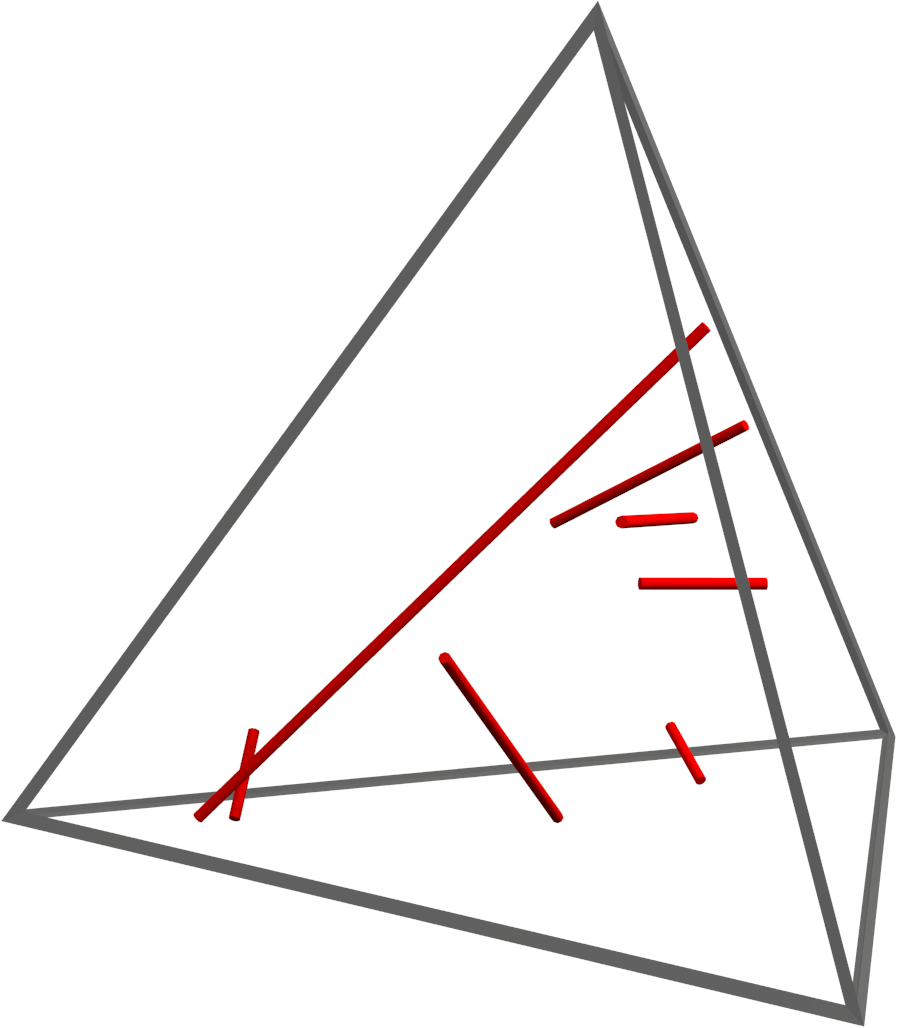
\includegraphics[width=0.5\columnwidth]{figures/7lines}
    \end{captionbeside}
\end{figure}
%
% subsection definition (end)

\subsection{Mathematical Properties} % (fold)
\label{sub:mathematical_properties}
%
We now examine the mathematical properties of tensor core lines.
%
We show that they are indeed structurally stable lines, and that in linear
tensor fields, these lines are always straight.
%

%
\begin{theorem}\label{thm:tcl_stable_lines}
In a $C^1$-continuous tensor field, tensor core lines are structurally stable
line structures that are either closed or end at the domain boundary.
\end{theorem}
%
To show \cref{thm:tcl_stable_lines}, we consider a local representation of a
real eigenvector field in the neighborhood of a point as a normalized vector
field.
%
Then the fact that the \ac{PV} operator gives such line
structures~\cite{Peikert1999} shows the theorem.
%
Note that although such a representation of an eigenvector field as a normalized
vector field is locally possible, it does not apply globally in a consistent
way, and therefore does not provide a strategy to extract tensor core lines.
%
We also mention that in real datasets, tensor cores may build surfaces or even
volumetric structures.
%
This is due to shape symmetries often observed in artificial data produced by
humans.
%
Even though these structures are unstable (adding noise destroys the surfaces to
many lines), our extraction algorithm has to deal with them.
%

%
\begin{theorem}
In linear tensor fields, tensor core lines are straight lines.
\end{theorem}
%
This follows from the fact that for linear tensor fields, the linear
approximation in \eqref{eq:lin_approx} describes the whole data set
exactly: if \eqref{eq:lin_cond} holds for a small $h$, it holds for all
$h$ (i.e., on a whole straight line) as well.
%
\Cref{fig:7lines} shows an example of a random linear tensor field containing
seven isolated tensor core lines.
%
% subsection mathematical_properties (end)
%

%
\section{Extracting Tensor Core Lines from Piecewise Linear Data} % (fold)
\label{sec:extracting_tensor_lines}
%
We assume tetrahedral partition of the three-dimensional domain.
%%
Each tetrahedron supports a linear piece if the given tensor field has a
constant tensor for each vertex.
%%
The gradient field $\nabla\mT$ consists of constant pieces per
tetrahedron.
%%

%
In general, tensor core structures are line features (see \cref{sec:tcl_theory}).
%%
We extract them by first bounding the search space to individual
tetrahedral cells and then to the cell boundary.
%%
The two-dimensional search on triangles reduces the extraction
generally to finding point features: the intersection of core lines
with the cell boundary.
%%
We will apply a root finding algorithm for feature extraction.
%%

%
This discretization of the field and also the restriction to a local
two-dimensional search space is applied similarly by other methods,
\eg, the Sujudi and Haimes extractor~\cite{Sujudi1995} or the extractor for
degenerate lines in tensor fields by Zheng and Pang~\cite{Zheng2004}.
%%
\subsection{General Algorithm}
%%
A tensor core line consists of all locations $\vx$ where
$\mT(\vx)\, \vr \parallel \vr$ and $\nabla_{\vr}\mT(\vx)\, \vr \parallel \vr$,
see \eqref{eq:tensor_line}.
%%
This can be expressed as solutions to
%%
\begin{equation}\label{eq:system}
\begin{aligned}
  (\mT(\vx)\,\vr) \times \vr &= \vNull\\
  (\nabla_{\vr} \mT(\vx)\, \vr) \times \vr &= \vNull~.
\end{aligned}
\end{equation}
%%
This system consists of six polynomial equations in the unknown
variables $\vx$ and $\vr\neq{}\vNull$.
%%

The polynomials are of maximum degree 1 in $\vx$ and 3 in $\vr$.
%%
Note that for a linear tensor field, $\nabla_{\vr}\mT(\vx)=\nabla_{\vr}\mT$ is
constant and thus independent of $\vx$.
%%
We parameterize directions $\vr$ such that they can be defined \wrt triangles.
%%
With the restriction of the local search space to triangles that bound
tetrahedra, the solution of the polynomial system is equivalent to
finding isolated (real) roots, \ie, points where all six polynomials
simultaneously become zero.
%%

%
We construct a bisection algorithm that uses the Bernstein-B\'ezier form
(\cref{sec:bb}) of the polynomials to exclude the presence of roots within
subtriangles.
%%
Within the search space (\cref{sec:searchspace}) a recursive
subdivision (\cref{sec:subdiv}) approximates the locations of roots in
$\vx$-$\vr$-space with an arbitrary user-defined precision.
%%
The local feature extraction is followed by a stage that clusters solutions and
then connects feature points to lines within cells (\cref{sec:cluster})
%
Finally, we use a filtering criterion for removing unstable solutions
(\cref{sec:filt}).
%
\subsection{Polynomial System in Bernstein-B\'ezier Form}
\label{sec:bb}
%%
We consider bivariate polynomials $p\,:\,\RRSet^2\rightarrow\RRSet$ of
degree $n$, which are evaluated in a triangular domain
$\Delta\subset\RRSet^2$.
%%
Let indices $i,j,k\geq{}0$.
%%
We write $p(\vu)$ in Bernstein-B\'ezier form as
%%
\begin{equation}\label{eq:bb}
\begin{aligned}
  p(\vu)~=\sum _{i+j+k=n} B^n_{ijk}(\vu)\,b_{ijk}~,\quad%
  B^n_{ijk}(\vu)~=~\frac{n!}{i!j!k!}\,a_1^i\,a_2^j\,a_3^k
\end{aligned}
\end{equation}
%%
with the bivariate Bernstein polynomials $B^n_{ijk}$ as basis and
coefficients (or B\'ezier control points) $b_{ijk}$.
%%
The basis is defined w.r.t. the barycentric coordinates
$a_\ell:=a_\ell(\vu)$, the linear polynomials that satisfy
%%
% \begin{equation}\label{eq:bc}
% \begin{aligned}
%   \sum _{\ell=1}^3 a_{\ell}(\vu)\,\vu_{\ell} = \vu\quad\text{and}\quad
%   \sum _{\ell=1}^3 a_{\ell}(\vu) = 1~.
% \end{aligned}
% \end{equation}
%%
\begin{equation}\label{eq:bc}
\begin{aligned}
a_1\vu_1+a_2\vu_2+a_3\vu_3 = \vu\quad\text{and}\quad
a_1+a_2+a_3 = 1
\end{aligned}
\end{equation}
\wrt triangle $\Delta$ spanned by vertices $\vu_1,\vu_2,\vu_3$
\cite{Hoschek1993}.
%%

%
The Bernstein-B\'ezier representation has a number of remarkable
properties.
%%
Important to our setting is the \emph{convex hull property}\/:
%%
For any $\vu\in\Delta$ -- or equivalently all barycentric coordinates
are nonnegative -- the value $p(\vu)$ is bounded by the convex hull
of the control points $b_{ijk}$.
%%
For scalar coefficients $b_{ijk}\in\RRSet$ this means that if either
all $b_{ijk}>0$ or all $b_{ijk}<0$ for $i+j+k=n$ then $p$
\emph{cannot} have a zero crossing (or real root) on $\Delta$.
%%
We use this criterion for an iterative subdivision of a triangle
$\Delta$ into smaller and smaller triangles that either may contain or
cannot contain a root.
%%
\subsection{Parameterization of the Search Space}
\label{sec:searchspace}
%%
The equations in the system~\eqref{eq:system} are polynomials in $\vx$
and $\vr$.
%%
This means the search space consists of two independent domains:
position and direction.
%%

%
As pointed out before, positions $\vx$ are restricted to points on
triangles bounding tetrahedral cells.
%%
For each triangle of a tetrahedron we represent positions $\vx$ in
barycentric coordinates \wrt this triangle.
%%
Barycentric coordinates are defined in \emph{local coordinates} of the triangle
and therefore have two degrees of freedom.
%%
After switching to barycentric coordinates the further steps, polynomial
evaluation and subdivision, are independent of the supporting triangle.
%%

%
We represent a direction vector $\vr$ as a point on a hemisphere.
%%
As not only its orientation (and thus sign) is irrelevant for
the system~\eqref{eq:system} but also its scale (as long as $\vr\neq{}0$), we
approximate the hemisphere by a triangulation.
%%
This way, we use the same parameterization and the same representation
for $\vx$ and $\vr$.
%%
We remark that there is no need for an ``accurate'' approximation of
the hemisphere.
%%
We simply use a four-sided open pyramid (see \cref{fig:subdivision_scheme}).
%%

%
\begin{figure}[t]
  \centering
  \setlength\figurewidth{\textwidth}
  \input{figures/algorithm_tikz}
  \caption{The search space is parameterized on triangles $\Delta_{\vx}$ in position
  space and $\Delta_{\vr}$ on the hemisphere of possible eigenvector directions.
  The figure shows a pair of triangles after several subdivision steps.}
  \label{fig:subdivision_scheme}
\end{figure}
%

%
For a given triangle, we have to consider a tensor field $\mT$ that is linear in
$\vx$ and a direction vector $\vr$ that is linearly interpolated on a triangle
of the ``hemisphere''.
%%
Then the left-hand-sides of the system~\eqref{eq:system} give three
polynomials that are linear in $\vx$ and quadratic in $\vr$ and three
polynomials that are cubic in $\vr$ as they don't depend on $\vx$
because $\nabla_{\vr}\mT$ is constant.
%%

%
Each of these six polynomials can be written in the form
%%
\begin{equation}\label{eq:polynomial}
  \begin{aligned}
    p(\vx,\vr)~=~%
    \sum _{\substack{i+j+k=1\\ \alpha+\beta+\gamma=3}}%
    B^1_{ijk}(\vx)\,B^3_{\alpha\beta\gamma}(\vr)\,%
    b_{ijk\,\alpha\beta\gamma}~.
  \end{aligned}
\end{equation}
%%
This is the tensor product of the interpolation in $\vx$ and $\vr$.
%%
It gives $3\times{}10=30$ coefficients $b_{ijk\,\alpha\beta\gamma}$.
%%
(All indices are nonnegative. Latin indices indicate position space,
Greek indices denote direction space.)
%
This form has degree 4 and can represent all polynomials in
system~\eqref{eq:system}.
%
We use this unified representation for didactic purposes.
%
Using the real number of degrees in $\vx$ and $\vr$ for each polynomial gives a
smaller number of coefficients (18 or 10).
%%
Note that position and direction are expressed in \emph{local coordinates}\/ (or
barycentric coordinates) of the triangles, such that $p$ depends on only four
coordinates in total.
%%
For the sake of a concise notation we write $p(\vx,\vr)$, $B^1_{ijk}(\vx)$
and $B^3_{\alpha\beta\gamma}(\vr)$.
%
\subsection{Root Finding by Subdivision}
\label{sec:subdiv}
%%
Algorithms for finding roots of B\'ezier curves and surfaces are
typically based on the convex hull property and use a recursive
bisection~\cite{Rockwood1989,Hoschek1993}.
%%
We adopt this technique.
%%
% We adopt the standard bisection algorithm
% \cite{Rockwood:1989:RRT,Hoschek1993} for finding roots of
% polynomial functions $\RRSet\rightarrow\RRSet$ that is based on the
% convex hull property of the Bernstein-B\'ezier representation of
% polynomials.
%%
The main differences in our setting are the fact that all six
equations in \eqref{eq:system} must be satisfied simultaneously and
that this is checked in two different two-dimensional domains:
position and space.
%%
\subsubsection*{Roots of One Single Polynomial}
%%
The system \eqref{eq:system} defines six polynomials.
%%
For the initialization of the algorithm, we need to determine the
Bernstein-B\'ezier form, \ie, the coefficients $b_{ijk\,\alpha\beta\gamma}$
in \cref{eq:polynomial}, for each of these polynomials.
%%
This can be done easily by sampling and interpolation:
%%
There are $3\times{}10$ coefficients and two triangular parameter
domains.
%%
As \cref{eq:polynomial} lives in a tensor-product space,
interpolation of position and direction can be separated.
%%
Chose $3$ or $10$ distinct sampling positions in $\Delta_{\vx}$ or
$\Delta_{\vr}$, respectively, and evaluate the values for the given
polynomial.
%%
Then interpolate these values using the Bernstein-B\'ezier basis.
%%
The interpolation conditions define a linear system that has a unique
solution.
%%
We remark that the choice of sampling positions can be arbitrary as
long as they are distinct.
%%
For polynomial degree $n$, we use the domain points
$\tfrac{1}{3}(i,j,k)$ with $i+j+k=n$ in barycentric coordinates.
%%
This ensures a well-conditioned system matrix.
%%
As the sampling positions are fixed, the system matrix is constant,
\ie, interpolation requires only inversion or factoring.
%%
So after sampling, the conversion to Bernstein-B\'ezier form reduces
to a linear transform than can be expressed as a matrix-multiplication.
%%

The outline of the subdivision algorithm is as follows.
%%
We are given a pair $(\Delta_{\vx},\Delta_{\vr})$
of position-direction parameter triangles and a polynomial in
Bernstein-B\'ezier form.
%%
The coefficients $b_{ijk\,\alpha\beta\gamma}$ indicate the absence of zero
crossing if they are either all positive or all negative.
%%
In this case, no root is found and processing of
$(\Delta_{\vx},\Delta_{\vr})$ stops.
%%
If there is any sign change or zeros in the coefficients, there
\emph{may} exist roots within the parameter space
$(\Delta_{\vx},\Delta_{\vr})$.
%%
In this case we \emph{subdivide}\/ one of the parameter triangles.
%%
We alternate between subdividing $\Delta_{\vx}$ in position-space and
$\Delta_{\vr}$ in direction-space.
%%
For both, we use a regular 1:4-split (see \cref{fig:subdivision_scheme}).
%%
Each of the four new subtriangles is processed recursively in the same
way.
%%

%
\subsubsection*{System of Polynomials}
%%
We explained the basic algorithm for a single polynomial.
%%
Solving system~\eqref{eq:system} means finding solutions $\vx,\vr$ where all six
polynomials become zero simultaneously.
%
We test each polynomial \emph{individually}.
%%
Only if there is a sign change in the coefficients for \emph{all}
polynomials, a simultaneous root can exist.
%%

%
Every level of subdivision restricts the parameter domain and thus
puts tighter bounds on the region that (potentially) contains a root.
%%
The subdivision stops either if there cannot be any root in
$(\Delta_{\vx},\Delta_{\vr})$ or when the magnitude of all polynomials
drops below a threshold (see below).
%%
In the latter case, we have found a root, and the barycenters of the
triangles define its location in parameter space.
%%

Similar to the initial interpolation, the Bernstein-B\'ezier form of
the subdivided polynomial can be evaluated by a linear transformation:
%%
Evaluate the polynomial at domain points in the new, smaller triangle
and apply interpolation.
%%
Evaluation and interpolation can be combined to one transformation for each
of the four new triangles.
%%

\subsubsection*{Solution and Stopping Criterion}
%%
All computations involving Bernstein-B\'ezier polynomials are done in
barycentric coordinates, which yields a concise implementation of the
algorithm.
%%
However, the barycentric coordinates are relative to the current
triangle, and we still need to keep track of the absolute positions of
its vertices in parameter space for bounding the regions of roots.
%%
This can be done with a small amount of bookkeeping by tracking the
subdivision steps such that any ``child'' triangle can be
reconstructed from its ``parent'' and ultimately from the initial
parameter triangle.
%%

%
We stop the subdivision when we are close enough to a root.
%%
We require the magnitude of all polynomials to drop below a threshold
simultaneously.
%%
For each polynomial its magnitude is bounded in
$(\Delta_{\vx},\Delta_{\vr})$, and we test
%%
\begin{equation}\label{eq:stop}
  \begin{aligned}
    |p|~<~%
    \varepsilon_{\mathrm{t}}\,\cdot\,\invn{\mT}_{\infty}~,
  \end{aligned}
\end{equation}
%%
where $|p|:=\max \{\, |b_{ijk\,\alpha\beta\gamma}| \,\}$ is an upper bound for
the magnitude of p in $(\Delta_{\vx},\Delta_{\vr})$.
%%
The magnitude of the tensor field in $\Delta_{\vx}$ is given as
%%
\begin{equation}\label{eq:magt}
  \begin{aligned}
    \invn{\mT}_{\infty}=\sup_{\vx\in\Delta_{\vx}} \{\,\invn{\mT(\vx)}\,\}
    = \max_i\{\, \invn{\mT_i} \,\}~,
  \end{aligned}
\end{equation}
%%
where $\mT_i$ denote the constant tensors at the triangle vertices
$i=1,2,3$, and $\invn{\mT_i}$ denotes their spectral norm.
%%

%
The parameter $\varepsilon_{\mathrm{t}}$ defines a \emph{relative}\/ threshold,
which is independent of the local magnitude $\invn{\mT}_{\infty}$ of the tensor
field within $\Delta_{\vx}$.
%%

\subsubsection*{Breadth-First Search Modification}
%%
%%
As we hinted at in \cref{sec:tcl_theory}, the symmetries and regular shapes
inherent to data such as stress simulations of mechanical parts often lead to
\eqref{eq:tensor_line} being fulfilled or almost fulfilled on surface- or
volume-type structures.
%%
Also there may be tensor core lines which do not intersect but which
are part of the domain triangle.
%%
In these cases the roots are no longer isolated points but algebraic
structures.
%%
As a consequence, the presented algorithm would not be efficient, as it would do
an exhaustive search for all ``points'' on the structure.
%%
In cases where the higher-order structures are disturbed by noise and break down
to lines, the algorithm still has to do a large number of subdivisions before
reaching a termination criterion.
%%

%
A simple modification of the algorithm enables detecting such cases:
%%
we apply a breadth-first search when looking for roots.
%%
In the implementation, we use a queue of pairs $(\Delta_{\vx},\Delta_{\vr})$ of
parameter regions with potential roots.
%%
If the number of elements in the queue exceeds a threshold $M$, we
assume that the solution to \eqref{eq:system} forms an algebraic
structure and terminate the local search.
%%
If the search is terminated for one of the initial triangles $\Delta_{\vr}$ that
tessellate the hemisphere, we still need to consider the other triangles,
because they may still contain isolated solutions.
%%

\subsection{Clustering and Line Connection}
\label{sec:cluster}
%%
The root finding returns a list of small parameter regions
$(\Delta_{\vx},\Delta_{\vr})$, which are assumed to contain a solution to
\eqref{eq:system}.
%%
The size of these triangles is steered by the threshold
$\varepsilon_{\mathrm{t}}$.
%%
Typically, the algorithm returns multiple regions that all refer to the same
solution due to numerical noise.
%%
For this reason, we apply a post-process that clusters such regions and selects
a unique representative $(\vx,\vr)$ for each solution.
%%

Given two representatives, we define the distance as the maximum of their
distances in position- and in direction space.
%%
We employ a simple single-linkage hierarchical clustering algorithm:
%%
We start with each parameter region as a single cluster.
%%
Two clusters are merged if the distance between any two elements from both
clusters is smaller than a clustering threshold $\varepsilon_{\mathrm{c}}$.
%%
We repeat this process until the number of clusters no longer changes.
%%
For each cluster, we select the triangle pair as a representative where $\max \{
|p_i| \}$ is smallest for all polynomials $i=1,\dots,6$.
%%
We select the center points of both triangles in this pair as the solution
represented by this cluster.
%%

This algorithm has a complexity of $\mathrm{O}(n^3)$ in the number of solution
candidates.
%%
Typically $n$ is small: less than $200$ candidates are found in the vast
majority of cases.
%%
At this scale, the performance impact of the clustering algorithm is negligible.
%

%%
For each tetrahedral cell of the dataset, we now connect the root points found
on its faces by a line segment.
%%
Since in piecewise linear fields, tensor lines are always straight within a cell
(see \cref{sec:tcl_theory}), we greedily connect the two points with the smallest
difference in eigenvector direction until no more pairs are left.
%%
Similar to the vortex core lines by Sujudi and Haimes \cite{Sujudi1995}, this
gives a set of discontinuous line segments.
%%
%
\subsection{Filtering}
\label{sec:filt}
%
If the dataset contains not only lines, but also surface- or volume-type
structures where eigenvector trajectories are locally straight, our algorithm
might still find isolated solutions on these structures.
%
These occur if the unstable structures are disturbed by noise.
%
To filter these spurious points, we measure the numeric stability of a solution
given its representative $(\vx, \vr)$ with
%%
%
\begin{equation}
  s(\vx, \vr) = \left|\det
      \begin{pmatrix}
          \frac{\nabla_{\vr_2}\mT(\vx)\,\vr}{\|\mT(\vx)\|_{\infty}} &
          \frac{\nabla_{\vr_1}\mT(\vx)\,\vr}{\|\mT(\vx)\|_{\infty}} &
          \vr
      \end{pmatrix}\right| \text{,}
\end{equation}
%
where $\vr, \vr_1, \vr_2$ are orthonormal.
%%

%
The stability $s(\vx, \vr)$ measures the directional change that the eigenvector
$\vr$ of the tensor $\mT(\vx)$ experiences when moving orthogonal to the tensor
core line.
%%
If this change is small, the magnitude of the determinant in $s$ will be small.
%%
This is an indicator that the line is numerically unstable.
%%
The normalization by $\|\mT(\vx)\|_{\infty}$ ensures the independence from the scale
of the tensor field.
%%

%
Filtering out lines with small numeric stability $s$ is a post-process that must
be done by a user.
%%
In practice, the distribution of $s$ over all found solutions shows an
exponential behavior.
%%
In order to facilitate choosing a threshold, we visualize $s$ on a logarithmic
scale.
%%
%%% Local Variables:
%%% mode: latex
%%% TeX-master: "../TensorCoreLines"
%%% End:
%

%
\section{Results} % (fold)
\label{sec:tcl_results}
%
We applied our algorithm to stress tensor fields obtained from structural
mechanics simulations of varying complexity.
%
The Cauchy stress tensor (often referred to as $\mathbf{\sigma}$ in mechanics
literature) is a symmetric tensor that desribes the local stress state of an
object experiencing small elastic deformations.
%
Its eigenvectors point in the directions of the principal stresses.
%
The sign of the eigenvalues indicate if the stress is compressive or tensile.
%
Swirling structures in stress tensor fields can result from torque induced in
part of a structure.
%
As we will show, it is not always intuitive where this will happen in a complex
structure subject to a load or deformation.
%
Computing tensor core lines allows an easy identification of these phenomena.
%
In this section, we present the results of our algorithm on several datasets, we
analyze its performance and parameter sensitivity, and we compare our results to
the toplogical skeleton formed by degenerate lines.
%
\subsection{Cylinder} % (fold)
\label{sub:torque_applied_to_a_cylinder}
%
In \cref{fig:tube_lines} we show the eigenvector trajectories resulting from
applying a torque around the long axis of a cylinder.
%
The yellow line visible in the center is the result of our algorithm applied to
this case after filtering out numerically unstable solutions.
%
These solutions occur because the third eigenvector, which is orthogonal to the
other two, points outwards from the center line everywhere in the domain.
%
This means that the trajectories of this eigenvector are straight lines
everywhere inside the cylinder.
%
Situations like this are common in stress tensor fields, and are handled in our
algorithm by the threshold $M$.
%
Nevertheless, single line segments with low numeric stability $s$ may occur due
to noise (see \cref{fig:unfiltered_lines}).
%
After filtering them out, the clear central line visible in
\cref{fig:tube_lines} remains.
%
% subsection torque_applied_to_a_cylinder (end)
%
\subsection{Handle} % (fold)
\label{sub:hook}
%
\begin{figure}[tp]
    \centering
    \setlength\figurewidth\textwidth
    \input{figures/hook_results_tikz}
    \caption{Tensor core lines for two different deformations in the
             \textsc{Handle} dataset. On the top, we show the resulting
             deformations. The von Mises stress $\sigma_{\textnormal{vM}}$ is
             color-coded on the surface. We represent the tensor core line as
             tubes in the undeformed coordinate system. Their color indicates
             the numerical stability $s$. The tensor field is shown for context
             using elliptical glyphs.}
    \label{fig:hooks}
\end{figure}
%
This case shows a handle-like structure with a right angle being deformed in
two different ways.
%
One end is fixed, while the other end experiences different displacements.
%
The first is a rotation around the shaft, which applies a torque to it.
%
The second includes an additional downward shift.
%
\Cref{fig:hooks} shows a tensor core line in the center of the shaft for both
cases.
%
Interestingly, a line is also visible in the ``handle''-part of the structure,
even though no direct torque was applied here.
%
The line in the handle shifts away from the plane of symmetry in the second
deformation case.
%
A look at the tensor field around the core lines confirms that they are indeed
the center of a swirling behavior of the tensor field.
%
% subsection hook (end)
%
\subsection{Truck Bumper} % (fold)
\label{sub:truck_bumper}
%
This case shows a load applied to the extreme end of the bumper of a cargo
truck.
%
Applying our algorithm to the dataset results in a large number of lines being
found all over the domain.
%
This may in part be explained by the low resolution of the simulation.
%
After applying a filter on the numeric stability $s$, two lines with high
stability stand out.
%
Somewhat counterintuitively, these are found on the side opposite to the end
experiencing the load.
%
In \cref{fig:truck_bumper}, we can clearly see the radial behavior of the
tensor field around both lines.
%
Finding these locations by manually inspecting the tensor field in detail would
be a tedious task.
%
Using the tensor core line extractor, they can be identified at a glance.
%
\begin{figure}[p]
    \centering
    \setlength\figurewidth\textwidth
    \input{figures/truck_bumper_results_tikz}
    \vspace*{-5mm}
    \caption{Tensor core lines in the \textsc{truck bumper} dataset. The
             deformation shown on the top left is scaled by a factor of
             \num{500} for illustrative purposes. The bottom shows detail views
             of two interesting lines with tensor glyphs for context.}
    \label{fig:truck_bumper}
\end{figure}
%
% subsection truck_bumper (end)
%
\subsection{Crane} % (fold)
\label{sub:crane}
%
In this dataset, the arm of a crane is exposed to a downward pull applied to
the lower side of a cube at the end (see \cref{fig:crane}).
%
Similar to the truck bumper, it is not intuitively clear in which parts of the
structure a swirling behavior of the tensors will occur, just from looking at
the setup of the case.
%
Almost all stable solutions we find are located in the diagonal rods on the
lower side.
%
Again, looking closely at the tensors around the core lines, we can see the
radial behavior.
%
\begin{figure}[p]
    \centering
    \setlength\figurewidth\linewidth
    \input{figures/crane_results_tikz}
    \vspace*{-7mm}
    \caption{Tensor core lines in the \textsc{Crane} dataset. The resulting
             deformation on the left is scaled by a factor of
             \num{1500}.}
    \label{fig:crane}
\end{figure}
%
% subsection crane (end)
%
\subsection{Spring} % (fold)
\label{sub:spring}
%
A simulation of a coil spring being compressed and slightly bent between two
plates is shown in~\cref{fig:spring}.
%
Apart from numerical noise in the poorly resolved plates, we find significant
tensor core lines at the center of the coil's cross-section.
%
A look at the tensor field visualized by glyphs reveals that in this case, we
do not have a simple swirling behavior of the tensors.
%
Instead, the tensor field shows something similar to a hyperbolic behavior in
vector fields.
%
In the rightmost picture in~\cref{fig:spring}, we can see that eigenvector
trajectories start at the wall on both sides and curve into the same direction.
%
This direction is reversed on the top and bottom side of the spring.
%
In the middle, there is a surface where these curves become straight lines along
the diameter of the cross-section.
%
This is exactly where we find a tensor core line.
%
\begin{figure}[p]
    \centering
    \setlength\figurewidth\linewidth
    \input{figures/spring_results_tikz}
    \vspace*{-5mm}
    \caption{Tensor core lines in the \textsc{Spring} dataset. We visualize the
             tensors near the core line with box glyphs in this case. They make
             it easier to see the hyperbolic behavior of the eigenvectors that
             occurs in the coil's cross-section. }
    \label{fig:spring}
\end{figure}
%
% subsection spring (end)
%
\subsection{Performance and Parameter Study} % (fold)
\label{sub:performance}
%
\begin{table}[p]
    \centering
    \caption{Performance of the algorithm for the datasets presented in this paper.}
    \begin{tabular}{lSSS}
        \toprule
        Dataset & {\# of cells/\num{e3}} & {time/\si{\second}} & {avg. time per face/\si{\milli\second}} \\% & avg. time/face (single core) [ms] \\
        \midrule
        \textsc{Cylinder} & 65 & 8 & 0.034 \\% & 0.14 \\
        \textsc{Handle} & 235 & 36 & 0.038 \\% & 0.16 \\
        \textsc{Truck Bumper} & 97 & 32 & 0.081 \\% & 0.36 \\
        \textsc{Crane} & 108 & 63 & 0.146 \\% & 0.59 \\
        \textsc{Spring} & 181 & 82 & 0.114 \\
        \bottomrule
    \end{tabular}\label{tab:performance}
\end{table}
%
The performance of our algorithm is dependent on the dataset.
%
If we find a large number of tensor core lines in the dataset, computation
will be slower as fewer cells can be discarded early.
%
We tested our algorithm using a consumer PC with a 4-core Intel Core i7 \ac{CPU}
at \SI{3.4}{\giga\hertz}.
%
Our implementation is parallelized over the faces of the dataset using
OpenMP~\cite{OMP2013}.
%
Performance numbers for the different datasets shown in this paper are presented
in \cref{tab:performance}.
%
To examine the dependence of the performance and results of our algorithm on the
parameters $M$, $\varepsilon_{\mathrm{t}}$ and $\varepsilon_{\mathrm{c}}$, we
conducted a parameter study.
%
We selected baseline parameters $M = 10^3$, $\varepsilon_{\mathrm{t}} =
\num{e-6}$ and $\varepsilon_{\mathrm{c}} = \num{e-3}$.
%
We then varied each parameter separately and applied our algorithm to the
cylinder dataset.
%
The results can be seen in \cref{fig:parameter_study}.
%
We can see that the performance is controlled by the threshold $M$, which
controls at which point we assume we are not converging onto an isolated
solution.
%
Increasing $M$ also increases the number of solutions we find.
%
However, if we look at the number of solutions that remain after filtering based
on numeric stability, it becomes clear that these solutions are only caused by
noise.
%
Increasing $M$ did not result in any additional numerically stable lines.
%
The parameters $\varepsilon_{\mathrm{t}}$ and $\varepsilon_{\mathrm{c}}$ have
almost no noticeable impact on runtime or solutions, unless we choose
unreasonable numbers.
%
In case of $\varepsilon_{\mathrm{t}}$, choosing a value that is larger than
\num{e-3} causes an explosion of the number of found solutions, as the
tolerance is not tight enough.
%
Choosing $\varepsilon_{\mathrm{c}}$ smaller than $\varepsilon_{\mathrm{t}}$
means that candidate solutions belonging to the same cluster often can not be
clustered, because the search radius is smaller than the distance between the
triangle centers.
%
Otherwise, $\varepsilon_{\mathrm{c}}$ is very stable.
%
This is because for solutions which are isolated points and belong to different
eigenvectors, the separation between clusters in direction space is rather
large.
%%
This means the choice of $\varepsilon_{\mathrm{c}}$ is not critical as
long as it is not chosen extremely small, or so large that solutions
which belong to different eigenvectors are clustered together.
%%

%
Stability tests on our other datasets all produced very similar results.
%
We recommend choosing $M = \num{e2}$, $\varepsilon_{\mathrm{t}} = \num{e-3}$ and
$\varepsilon_{\mathrm{c}} = \num{e-2}$ if performance is important.
%
If accuracy is important, we found that choosing stricter tolerances than $M =
\num{e3}$, $\varepsilon_{\mathrm{t}} = \num{e-6}$ and $\varepsilon_{\mathrm{c}}
= \num{e-3}$ does not produce noticeably better results.
%
\begin{figure}[t]
    \centering
    \tikzset{external/export=false}
    \input{figures/parameters_cylinder_tikz}
    \caption{
        Run times (\protect\tikz{\ref{plt:runtime}}) and number of found lines
        in the \textsc{Cylinder} dataset for various different parameters. We
        show the total number of lines found
        (\protect\tikz{\ref{plt:total_lines}}) and the number of lines remaining
        after filtering out numerically unstable lines
        (\protect\tikz{\ref{plt:filtered_lines}}). }
    \label{fig:parameter_study}
    \tikzset{external/export=true}
\end{figure}
%
\begin{figure}[p]
    \centering
    \setlength\figurewidth\columnwidth
    \input{figures/unfiltered_lines_tikz}
    \vspace*{-5mm}
    \caption{Results of our algorithm on the \textsc{Cylinder} dataset for
             different choices of $M$. Increasing $M$ results in more
             numerically unstable lines being found. If we filter them out, the
             result is virtually identical.}
    \label{fig:unfiltered_lines}
\end{figure}
%
% subsection performance (end)
%
\subsection{Comparison with Degenerate Lines} % (fold)
\label{sub:comparison_with_degenerate_lines}
%
Tensor core lines are mathematically distinct from degenerate lines where two or
more eigenvalues are equal.
%
The criterion for finding tensor core lines is completely independent of the
eigenvalues of the tensor field.
%
However, when looking at our results in stress tensor fields, one might wonder
if tensor core lines coincide with degenerate lines in practice.
%
To investigate this, we extracted degenerate lines from our datasets using the
method presented by Zheng and Pang \cite{Zheng2004}.
%
In stress tensor fields, degenerate lines mark locations where no unique
principal directions of stress can be established.
%
We found that tensor core lines and degenerate lines sometimes coincide, but
neither is a subset of the other.
%
In the \textsc{Crane} dataset, degenerate lines are found near the center of the
lower diagonal rods, where we also find tensor core lines.
%
However, a lot of degenerate lines are also found in regions where no tensor
core lines are located.
%
In the \textsc{Truck Bumper} dataset, a degenerate line coincides with one of
the two most significant tensor core lines we find, but not the other one.
%
Closeups of both datasets are shown in~\cref{fig:topo_comparison}.
%
In several datasets, such as the \textsc{Cylinder} and \textsc{Handle}, Zheng
and Pang's method fails to locate any degenerate lines at all.
%
\begin{figure}[p]
    \begin{captionbeside}{Comparison of unfiltered tensor core lines
    (red/yellow) and degenerate tensor lines (blue) for the \textsc{Truck
    Bumper} and \textsc{Crane} dataset. The red box marks the
    coincidence of a numerically stable tensor core line with a degenerate
    tensor line.\label{fig:topo_comparison}}
        \setlength{\figurewidth}{0.7\textwidth}
        \input{figures/topo_comparison_tikz}
    \end{captionbeside}
\end{figure}
%
% subsection comparison_with_degenerate_lines (end)
%
% section results (end)
%
\Todo[inline]{Add section explaining how to compute PEV and degenerate lines
with the same algorithm}
%
%
\section{Discussion} % (fold)
\label{sec:tcl_discussion}
%
We introduced tensor core lines as a new feature of second-order tensor fields.
%
It enables the quick detection of swirling behavior in tensor field lines.
%
Such behavior might not have a distinct physical meaning in all applications.
%
However, finding core lines helps to understand the structure of the tensor
field by breaking down a complex feature into a simple line structure that can
be easily visualized.
%
In this regard, our method fits in well with other feature-based visualization
methods.
%

%
Our method is a direct extension of the Sujudi/Haimes method for the extraction
of vortex core lines in vector fields.
%
As such, it shares many of its advantages and drawbacks.
%
The criterion is completely local and does not require integration.
%
As such, it is well parallelizable and not vulnerable to accumulating numerical
errors.
%
Still, we are hardly able to reach interactive run times, as we need to perform
an exhaustive search in a \ac{5D} space.
%
Like Sujudi/Haimes, we perform a search on piecewise linear data, which results
in straight lines within cells and discontinuities of the tensor core lines at
cell boundaries.
%
Using higher-order interpolation of the tensor field would help finding
continuous lines.
%

%
We have chosen to focus on piecewise linear tensor fields where each tensor
component is interpolated independently.
%
While alternative interpolation schemes have been proposed~\cite{Kindlmann2007},
component-wise interpolation is still widely used as a standard approach for
both tensor- and vector fields.
%

%
Unlike Sujudi/Haimes, we have no way of explicitly ensuring our solutions show
only swirling behavior by restricting them to regions where the derivative has
complex eigenvalues.
%
The derivative of the tensor field $\nabla \mT$ is a third-order tensor, for
which the definition of eigenvalues and eigenvectors is non-trivial
\cite{Zheng2007}.
%
This means that we also find structures similar to hyperbolic trajectories in
vector fields \cite{Machado2013,Machado2016}.
%
Further research is necessary in order to distinguish these different types of
features.
%

%
We introduced a measure for the numeric stability of tensor core lines.
%
Unfortunately, filtering out numerically unstable solutions must be done as an
interactive post-processing step, as the threshold is different for each
dataset.
%
It is worth investigating if this process can be automated.
%
Nevertheless, the measure enables us to distinguish significant and
insignificant solutions, which is a very useful tool for assessing the result of
our algorithm.
%

%
Our algorithm is numerically very stable.
%
We have three free parameters, two of which can be chosen in a wide range
without significant influence on the results, as we show in
\cref{sub:performance}.
%
The parameter $M$, which influences run time the most, can be chosen the same
for most datasets and as such does not require fine-tuning either.
%

%
Our algorithm is only designed for extracting structurally stable line
features, but surfaces or regions where the zero curvature criterion is
almost fulfilled seem to be common in real-world stress tensor data.
%
This might be due to the common occurrence of symmetries and regular shapes in
human-made objects, which are most frequently the focus of structural analysis.
%
It would therefore be interesting to investigate if these structures can
explicitly be extracted, possibly by restricting the search space to the edges
of tetrahedral cells.
%

%
Finally, it is worth noting that neither the formal definition of tensor core
lines nor the extraction algorithm poses any restrictions on the tensor field,
except that it be differentiable.
%
As such, it might also be used on indefinite tensor data, such as the Jacobian
of a vector field.
%
Finding applications outside of stress tensor analysis is a subject for further
research.
%
%
% chapter tensor_core_lines (end)
%
\chapter{Conclusion} % (fold)
\label{cha:tensor_vis_conclusions}
%
\lettrine[lhang=0.06, loversize=-0.015, findent=-1pt, nindent=3pt]{I}{n the previous} two
chapters, we extend the idea of a class of feature-based visualization
techniques for vector- and scalar fields to the realm of tensor fields.
%
In \cref{cha:parallel_eigenvectors}, we establish the \ac{PEV} operator as a
direct extension of the generic \ac{PV} operator.
%
It finds all locations where two tensor fields have parallel real eigenvectors.
%
Using this, we translate the concept of vortex core lines to their counterpart
in tensor fields in \cref{cha:tensor_core_lines}.
%
These tensor core lines mark the centers of ``swirling'' behavior of tensor
field lines.
%
Feature lines of this type can be extracted from piecewise linear data by
determining their intersections with the boundaries of tetrahedral cells.
%
The search for such intersections is a search for roots of higher-order
polynomials, which we solve using a recursive subdivision algorithm based on
their Bernstein-B\'ezier form.
%
The intersections are then connected to lines afterwards.
%

%
The work presented in this part of the thesis is basic research into
higher-order features in tensor fields.
%
As an application area, we focus on the visualization of stress tensor fields
from solid mechanics simulations.
%
In-detail analysis of the topology and structure of stress tensor fields still
is not well established within the solid mechanics community.
%
One reason for this might be that tensor fields are even more complex than
vector fields, which are already challenging to visualize and understand.
%
The \ac{PEV} operator and tensor core lines are additions to the visualization
toolbox that help to better understand the complex ways in which forces act in
solid materials.
%
Such feature-based techniques break down complex behavior into simple geometric
primitives that are more easily parsed and understood.
%
Maybe the development of more such techniques can help to better establish
tensor field visualization with solid mechanics researchers.
%
% chapter tensor_vis_conclusions (end)
%
% part tensor_vis (end)
%
\addpart{Appendix}
% \label{part:appendix}
%
\appendix\appendixtrue
%
\chapter{Interpolating the Transformation for New Surface Patches} % (fold)
\label{sec:transform_interpolation}
%
\lettrine[lhang=0.06, loversize=-0.015, findent=-1pt]{I}{n
\cref{sub:reconstructing_tangential_surface_deformation}}, we explain how to
reconstruct the tangential deformation experienced by a micro-patch over a
finite time interval $[t_\mathrm{s}, t_\mathrm{e}]$, if that patch has existed
for this whole interval.
%
If instead the patch was created at time $t_k > t_\mathrm{s}$ as one of the
outer patches during a split operation, we have to estimate the deformation it
has experienced until that time from its parent patch.
%
If the deformation across the parent patch was completely uniform, we could just
pass this deformation on to the child patches after a split.
%
However, in general there will be slight differences in the transformations
each of the four ghost particles have experienced.
%
At the time of the split, we still have this information for the time interval
since the parent patch was last reset (or first created).
%

%
Let $\vx_i(t_{k-1})$ be the positions of the ghost particles (relative to the
central point) at the last reset of the parent patch, or at the start time
$t_\mathrm{s}$ if the patch was not reset since that time.
%
Let $\vx_i(t_k)$ be the ghost particle positions at the time of the split.
%
Then $\mE_{t_{k-1}}^{t_k}$ obtained via \eqref{eqn:deformation_reconstruction}
can be thought of as the solution of the system
%
{\small
\begin{gather}
    \begin{pmatrix}
        \T{\vb_1(t_{k-1})} \\
        \T{\vb_2(t_{k-1})} \\
        \T{\vn(t_{k-1})}
    \end{pmatrix}
    \T{\left(\mE_{\,t_{k-1}}^{\,t_k}\right)}
    =
    \begin{pmatrix}
        \T{\vb_1(t_k) }\\
        \T{\vb_2(t_k)} \\
        \T{\vn(t_k)}
    \end{pmatrix}\\
    \vb_1(t) = (\vx_1(t) - \vx_2(t))/2 \\
    \vb_2(t) = (\vx_3(t) - \vx_4(t))/2\, \text{.}
\end{gather}
}
%
In other words, $\mE_{\,t_{k-1}}^{\,t_k}$ is the average of the transformations
that map the corresponding ghost particles to each other exactly.
%
\begin{figure}[t]
    \centering
    \setlength{\figurewidth}{0.9\linewidth}
    %
%
\begin{tikzpicture}[
	font=\small,
	thick,
	scale=\figurewidth/1cm*0.13,
	line join=round]
\tikzstyle{ghostparticle} = [fill=white, arrows=-o]
\tikzstyle{b1style} = [mycolor4, arrows=-latex]
\tikzstyle{b2style} = [mycolor1, arrows=-latex]
\tikzstyle{b1dstyle} = [very thick, mycolor4!50, arrows=-latex]
\tikzstyle{b2dstyle} = [very thick, mycolor1!50, arrows=-latex]
\tikzstyle{ellipse1style} = [mycolor3!70]
\tikzstyle{ellipse2style} = [mycolor2!70]

\coordinate (center1) at (0, 0);
\coordinate (x1) at (1.5, 0.15);
\coordinate (x2) at (-1, -0.1);
\coordinate (x3) at (0.15, 1.5);
\coordinate (x4) at (-0.1, -1);
\coordinate (b1) at (1.25, 0.125);
\coordinate (b2) at (0.125, 1.25);
\coordinate (vx) at ($ (center1)!2/3!(b1) + (center1)!2/3!(b2)$);

% normal
% \draw [fill=black, arrows=-latex]
% 	(center1) -- (0, 0, 1) node [below left] {$\vn$};

\fill [ellipse1style] (center1) circle [radius=0.4];
\fill [ellipse2style] (vx) circle [radius=0.4];

\node [below right] at (center1) {$\vx$};

\draw [ghostparticle] (center1) -- (x1) node [above] {$\vx_1$};
\draw [ghostparticle] (center1) -- (x2) node [left] {$\vx_2$};
\draw [ghostparticle] (center1) -- (x3) node [above] {$\vx_3$};
\draw [ghostparticle] (center1) -- (x4) node [below] {$\vx_4$};

\draw [b1style] (center1) -- (b1) node [below left] {$\vb_1$};
\draw [b2style] (center1) -- (b2) node [below left] {$\vb_2$};


\draw [b1dstyle] (center1) -- ($ (center1)!2/3!(b1) $)
		node [above, pos=0.6] {$a$};
\draw [b2dstyle, shorten >=0.1cm] ($ (center1)!2/3!(b1) $) --
		($ (center1)!2/3!(b1) + (center1)!2/3!(b2)$)
		node [left, pos=0.4] {$b$};

\draw [fill=black] (vx) circle [radius=0.08]
		node [right, xshift=0.05cm] {$\vx'$};

\begin{scope}[shift={(3.5, 0)}]
	\coordinate (center2) at (0, 0);
	\coordinate (x1) at (2, -1);
	\coordinate (x2) at (-1, 0.5);
	\coordinate (x3) at (2, 1);
	\coordinate (x4) at (-1, -0.5);
	\coordinate (b1) at (1.5, -0.75);
	\coordinate (b2) at (1.5, 0.75);
	\coordinate (vx2) at ($ (center2)!2/3!(b1) + (center2)!2/3!(b2)$);

	% normal
	% \draw [fill=black, arrows=-latex]
	% 	(center2) -- (0, 0, 1) node [below] {$\vn$};
	\fill [ellipse1style] (center2) circle [x radius=0.5, y radius=0.4];
	\fill [ellipse2style] (vx2) circle [x radius=0.6, y radius=0.4];

	\node [below] at (center2) {$\vx$};

	\draw [ghostparticle] (center2) -- (x1) node [right] {$\vx_1$};
	\draw [ghostparticle] (center2) -- (x2) node [left] {$\vx_2$};
	\draw [ghostparticle] (center2) -- (x3) node [right] {$\vx_3$};
	\draw [ghostparticle] (center2) -- (x4) node [left] {$\vx_4$};

	\draw [b1style] (center2) -- (b1) node [below left] {$\vb_1$};
	\draw [b2style] (center2) -- (b2) node [above left] {$\vb_2$};

	\draw [b1dstyle] (center2) -- ($ (center2)!2/3!(b1) $)
			node [above right, pos=0.6] {$a$};
	\draw [b2dstyle, shorten >=0.1cm] ($ (center2)!2/3!(b1) $) -- (vx2)
			node [above left, pos=0.4] {$b$};

	\draw [fill=black] (vx2) circle [radius=0.08]
		node [right, xshift=0.05cm] {$\vx'$};
\end{scope}

\draw [very thick, ellipse1style, shorten <=0.6cm, shorten >=0.6cm, arrows=-latex]
		(center1) to[out=-45, in=225]
			node [below, midway, text=black, yshift=-0.1cm] {$\mE$}
		(center2);

\draw [very thick, ellipse2style, shorten <=0.6cm, shorten >=0.7cm, arrows=-latex]
		(vx) to[out=25, in=145]
			node [above, midway, text=black, yshift=0.1cm] {$\mE'$}
		(vx2);

\end{tikzpicture}
    \tikzset{external/export=false}
    \caption{
        Interpolating the transformation at an offset position $\vx'$.
        The ghost particles in the direction of $\vx'$ have been stretched more
        than their counterparts during the time interval. Therefore the
        interpolated $\mE'$ has a stronger stretching effect on the local
        neighborhood of $\vx'$
        (\protect\tikz[baseline=-0.5ex]{
        \protect\fill[mycolor2!70] circle [radius=1ex];})
        than $\mE$ stretches the
        local neighborhood of $\vx$
        (\protect\tikz[baseline=-0.5ex]{
        \protect\fill[mycolor3!70] circle [radius=1ex];}).
        }
    \label{fig:interpolate_base_vectors}
    \tikzset{external/export=true}
\end{figure}
%

%
For the central point, it makes sense to weight those transformations equally,
but if we want to initialize a new patch whose center is slightly offset, we
get a more accurate result if we adjust the weights depending on where the
new center is located.
%
For this purpose, we parameterize the tangent space of the micro-patch by
expressing it as a linear combination of the two base vectors $\vb_1(t)$ and
$\vb_2(t)$.
%
We can now express the location of the new center $\vx'$ in this new basis:
%
\begin{equation*}
    \vx' = \lambda_1 \vb_1(t_k) + \lambda_2 \vb_2(t_k)\, \text{.}
\end{equation*}
%
These coordinates correspond directly to the coordinates of
$(\mE_{\,t_{k-1}}^{\,t_k})^{-1} \vx'$ at time $t_{k-1}$:
%
\begin{equation*}
    (\mE_{\,t_{k-1}}^{\,t_k})^{-1} \, \vx'
      = \lambda_1 \vb_1(t_{k-1}) + \lambda_2 \vb_2(t_{k-1})\, \text{.}
\end{equation*}
%
If $\lambda_1$ is positive, \ie, if $\vx'$ is located more towards $\vx_1(t_k)$
than towards $\vx_2(t_k)$, we want $\vx_1(t_k)$ to have a stronger influence on
the result.
%
The same applies to the direction of $\vb_2$.
%
We therefore compute new interpolated base vectors $\vb'_{1,2}(t)$ by weighting
the ghost particle positions with $\lambda_1$ and $\lambda_2$:
%
{\small
\begin{align}
    \vb'_1(t) =& (1+2\lambda_1) \, \vx_1(t) - (1-2\lambda_1) \, \vx_2(t) \\
    \vb'_2(t) =& (1+2\lambda_2) \, \vx_3(t) - (1-2\lambda_2) \, \vx_4(t)
        \, \text{.}
\end{align}
}
%
The adjusted transformation ${\mE_{\,t_{k-1}}^{\,t_k}}'$ is then the solution to
the system
%
{\small
\begin{equation}
    \begin{pmatrix}
        \T{\vb'_1(t_{k-1})} \\
        \T{\vb'_2(t_{k-1})} \\
        \T{\vn(t_{k-1})}
    \end{pmatrix}
    \T{\left({\mE_{\,t_{k-1}}^{\,t_k}}'\right)}
    =
    \begin{pmatrix}
        \T{\vb'_1(t_k)} \\
        \T{\vb'_2(t_k)} \\
        \T{\vn(t_k)}
    \end{pmatrix}\, \text{.}
\end{equation}
}
%
The complete transformation of a micro-patch that has been split off from a
parent at some intermediate time $t_k$ is then obtained by
%
\begin{equation}
    \mE_{\,t_\mathrm{s}}^{\,t_\mathrm{e}} = \mE_{\,t_n}^{\,t_\mathrm{e}} \cdot
                      \mE_{\,t_{n-1}}^{\,t_n} \cdot \; \cdots \; \cdot
                      \mE_{\,t_k}^{\,t_{k+1}} \cdot
                      {\mE_{\,t_{k-1}}^{\,t_k}}' \cdot
                      \mE_{\,t_\mathrm{s}}^{\,t_{k-1}}\, \text{.}
\end{equation}
%
Here, $\mE_{\,t_\mathrm{s}}^{\,t_{k-1}}$ is the transformation of the parent
patch from the start of the interval up to the time when its ghost particles
were last reset before the split operation at $t_k$.
%
If $t_\mathrm{s} > t_{k-1}$, it is omitted.
%
${\mE_{\,t_{k-1}}^{\,t_k}}'$ is the estimated transformation at a point with a
slight offset from the center of the parent patch in the interval before the
split.
%
% section interpolating_the_transformation_for_new_patches (end)

%
\chapter[Proof that PEV Yields Structurally Stable Curves]
    {Proof that the Parallel Eigenvectors Operator Yields Structurally Stable
    Curves} % (fold)
\label{cha:proof_pev_stable_lines}
%
\lettrine[lhang=0.06, loversize=-0.015, findent=-1pt]{I}{n
\cref{sec:pev_theory}}, we formulated \cref{thm:pev_stable_lines}, which states
that the \ac{PEV} operator yields structurally stable curves that are either
closed or end at the domain boundary.
%
We give the proof for this theorem here.
%
This proof was derived and written by Holger Theisel.
%

%
The main idea to prove \cref{thm:pev_stable_lines} is to search for \ac{PEV}
lines not in \ac{3D} $(x,y,z)$ space but in a \ac{6D} $(x,y,z,u,v,w)$ space:
%
at every point $\vx=\T{(x,y,z)}$, all vector directions $\vr=\T{(u,v,w)}$ are
checked for being an eigenvector of $\mS$ and $\mT$.
%
This means that we search for all \ac{6D} points $\T{(\vx,\vr)}$ fulfilling
$\mS(\vx)\, \vr \times \vr = \vNull$ and $\mT(\vx)\, \vr \times \vr = \vNull$.
%
We formulate this to search for all \ac{6D} points $\T{(\vx,\vr)}$ where a
\ac{6D} vector field $\overline{\vh}$ vanishes:
%
\begin{equation}
    \label{eq:theory_1}
    \overline{\vh}(\vx,\vr) =
        \begin{pmatrix}
            \mS(\vx) \, \vr \times \vr \\
            \mT(\vx) \, \vr \times \vr
        \end{pmatrix}
    = \overline{\vNull}\,\text{,}
\end{equation}
%
where $\overline{\vNull}$ is the zero vector in \ac{6D}.
%

%
Suppose a point $\T{(\vx_0,\vr_0)}$ is on a \ac{PEV} structure, \ie, fulfills
\cref{eq:theory_1}.
%
In order to study the \ac{PEV} structures in a linear neighborhood of
$\T{(\vx_0,\vr_0)}$, we search for all directions $\T{(d \vx,d \vr)}$ in which
$\overline{\vh}$ remains zero: $\nabla \overline{\vh} \cdot \T{(d \vx,d \vr)} =
\overline{\vNull}$.
%
In other words: we have to explore the null space of $\nabla \overline{\vh}$.
%
Applying elementary differentiation rules gives
%
\begin{equation} \label{eq:theory_2}
    \nabla \overline{\vh} =
        \begin{pmatrix}
            \mG_1 &   \mG_3 \\
            \mG_2 &   \mG_4
        \end{pmatrix}
        \,\text{,}
\end{equation}
%
with
%
\begin{equation} \label{eq:theory_3}
\begin{aligned}
    \mG_1 & =
        \begin{pmatrix}
            \mS_x \, \vr \times \vr &
            \mS_y \, \vr \times \vr &
            \mS_z \, \vr \times \vr
        \end{pmatrix}
        \,\text{,}
    \\
    \mG_2 & =
        \begin{pmatrix}
            \mT_x \, \vr \times \vr  &
            \mT_y \, \vr \times \vr  &
            \mT_z \, \vr \times \vr
        \end{pmatrix}
        \,\text{,}
    \\
    \mG_3 & =
        \begin{pmatrix}
        \mS \, \ve_1 \times \vr +  \mS \, \vr \times \ve_1 &
        \mS \, \ve_2 \times \vr +  \mS \, \vr \times \ve_2 &
        \mS \, \ve_3 \times \vr +  \mS \, \vr \times \ve_3
        \end{pmatrix}
        \,\text{,}
    \\
    \mG_4 & =
        \begin{pmatrix}
        \mT \, \ve_1 \times \vr +  \mT \, \vr \times \ve_1 &
        \mT \, \ve_2 \times \vr +  \mT \, \vr \times \ve_2 &
        \mT \, \ve_3 \times \vr +  \mT \, \vr \times \ve_3
        \end{pmatrix}
    \, \text{,}
\end{aligned}
\end{equation}
%
where $\mS_{x, y, z}$ and $\mT_{x, y, z}$ are partial derivatives of the tensor
fields and $\ve_i$ are unit vectors along the coordinates. Then
%
\begin{equation} \label{eq:theory_4}
   \T{\mG_1} \, \vr \; =\;  \T{\mG_2} \, \vr\; =\; 0 \,\text{,}
\end{equation}
%
and from \cref{eq:theory_1} follows
%
\begin{equation} \label{eq:theory_5}
   \T{\mG_3} \, \vr \;=\; \T{\mG_4} \, \vr \;=\;  0 \, \text{,}
\end{equation}
and
\begin{equation} \label{eq:theory_5a}
   \mG_3 \, \vr \;=\; \mG_4 \, \vr \;=\; 0 \, \text{.}
\end{equation}
%
\Cref{eq:theory_4,eq:theory_5} give that
%
\begin{equation} \label{eq:theory_6}
   \Rank{\nabla \overline{\vh}} = 4
\end{equation}
%
in the structurally stable case.
%
This means that for $\Rank{\nabla \overline{\vh}} < 4$, adding noise to $\mS,
\mT$ brings $\Rank{\nabla \overline{\vh}}$ to $4$.
%
\Cref{eq:theory_6} means that the \ac{PEV} structure around $\T{(\vx_0,\vr_0)}$
is a 2-manifold in \ac{6D}.
%
To see \cref{eq:theory_6}, we consider a rotation of the underlying coordinate
system such that $\vr=(0,0,r_z)$.
%
Then \cref{eq:theory_4,eq:theory_5} give that the rotated tensors
$\mG_1,\mG_2,\mG_3,\mG_4$ have vanishing third columns.
%
This and \cref{eq:theory_1} gives that $\nabla \overline{\vh}$ has two columns,
which proves \cref{eq:theory_6}.
%

%
One vector in the null space of $\nabla \overline{\vh}$ is trivial and denotes a
simple scaling of $\vr$:
%
\Cref{eq:theory_4,eq:theory_5,eq:theory_5a}
give $\nabla \overline{\vh}
\cdot \T{(\vNull, \vr)} = \overline{\vNull}$.
%
This means that the projection of the null space of $\nabla \overline{\vh}$ into
the spatial subspace $\vx$ gives a one-manifold in \ac{3D}.
%
This shows that \ac{PEV} gives line structures in \ac{3D}.
%
To show that they are closed, we consider the 6 components of $\nabla
\overline{\vh}$ as scalar fields and interpret the \ac{PEV} structure as
intersection of their \ac{5D} iso-hypersurfaces.
%
Iso-hypersurfaces are always closed, which means their intersections are also
closed.
%

%
Note that the proof did not make any assumptions on the behavior of $\mS, \mT$
around $\T{(\vx_0,\vr_0)}$.
%
This means that it holds also in case of a transition from real to imaginary
eigenvectors of $\mS$ or $\mT$ as well as in regions of isotropic tensors.
%
%

\backmatter

\printbibliography[heading=bibintoc]

\end{document}